% ------ DEFINIMOS DATOS DEL DOCUMENTO ------
\documentclass[spanish, 12pt, oneside]{Thesis}  
% Use the "Thesis" style, based on the ECS Thesis style by Steve Gunn
\usepackage[spanish,activeacute]{babel}
\graphicspath{ThesisFigs/}  % Location of the graphics files (set up for graphics to be in PDF format)
\usepackage[utf8]{inputenc}
% \usepackage[linesnumbered,lined,boxed,commentsnumbered]{algorithm2e}
\usepackage{algorithm}
\usepackage{algpseudocode}
%\usepackage{subfig}
\usepackage{float}

% ----- INICIO IMPORTACION DE PAQUETES ------
%\usepackage[round]{natbib}
\usepackage{epsfig}
\usepackage{colortbl}
% Include any extra LaTeX packages required
%\usepackage[square, numbers, comma, sort&compress]{natbib}  % Use the "Natbib" style for the references in the Bibliography
\usepackage[natbibapa]{apacite}
\usepackage{verbatim}  % Needed for the "comment" environment to make LaTeX comments
\usepackage{vector}  % Allows "\bvec{}" and "\buvec{}" for "blackboard" style bold vectors in maths
\hypersetup{urlcolor=black, colorlinks=true}  % Colours hyperlinks in blue, but this can be distracting if there are many links.
\usepackage{mathtools}
\usepackage{amsmath}
\usepackage{mathrsfs}
\usepackage{fancyhdr}
\usepackage{nomencl}
%\usepackage{float}
\usepackage[left]{lineno}
\usepackage[titletoc]{appendix}
\usepackage{graphicx}
%\usepackage{caption}
%\usepackage{subfigure}
\usepackage[export]{adjustbox}
\usepackage{wrapfig}
\usepackage{standalone}
\usepackage{tikz}
\usetikzlibrary{shapes,arrows,calc,positioning,arrows.meta,shapes.geometric,
    fit}
\usetikzlibrary{babel}
\usepackage{color}
\usepackage{multirow}
\usepackage{enumitem}
\usepackage{listings}
\usepackage{rotating}
% Agregado para girar a horizontal una pagina.
\usepackage{pdflscape}
% Agregado para insertar pdf en latex.
\usepackage{pdfpages}
%\usepackage{colortbl}
\usepackage{slashbox}
\usepackage{longtable}
\usepackage[inkscapelatex=false]{svg}
\usepackage{placeins}
\usepackage{needspace}

\usepackage{lineno}

\definecolor{mylightblue}{RGB}{059,131,189}
\definecolor{mygreen}{RGB}{040,114,051}
\definecolor{myblue}{RGB}{062,095,138}
\definecolor{mygray}{RGB}{156,156,156}
\definecolor{myorange}{RGB}{255,128,0} 

%  ESPANIOL
%\usepackage[spanish]{babel}
%\usepackage{algorithm}
%\usepackage{algpseudocode}

%\addto\captionsspanish{%
%  \renewcommand{\algorithmname}{Algoritmo}
%}
\makeatletter
\renewcommand{\ALG@name}{Algoritmo}
\makeatother

%Acento
%\usepackage[utf8]{inputenc} 
\usepackage[T1]{fontenc}
%

%%%%%%%
% En el preámbulo:

% Declaración del entorno:
%\theoremstyle{definition}
%\newtheorem{definition}{Definición}[section]

%%%%%%%%%%%%

\tikzstyle{intt}=[draw,text centered,minimum size=6em,text width=5.25cm,text height=0.34cm]
\tikzstyle{intl}=[draw,text centered,minimum size=2em,text width=2.75cm,text height=0.34cm]
\tikzstyle{int}=[draw,minimum size=2.5em,text centered,text width=3.5cm]
\tikzstyle{intg}=[draw,minimum size=3em,text centered,text width=6.cm]
\tikzstyle{sum}=[draw,shape=circle,inner sep=2pt,text centered,node distance=3.5cm]
\tikzstyle{summ}=[drawshape=circle,inner sep=4pt,text centered,node distance=3.cm]
\tikzstyle{decision} = [draw,shape=diamond, fill=blue!20, text width=6em, text badly centered, node distance=3cm, inner sep=0pt]

\usepackage{varioref}
%\usepackage[tablename=Tabla]{caption}
\usepackage{tabularx}
\usepackage{array}
\setlength\unitlength{20pt}
\usepackage{pst-plot}
\addtopsstyle{gridstyle}{gridlabels=0pt,griddots=0}
% ----- FIN IMPORTACION DE PAQUETES

%% ----------------------------------------------------------------
\newcommand{\abbrlabel}[1]{\makebox[3cm][l]{\textbf{#1}\ }}
\newenvironment{abbreviations}{
    \begin{list}{}
    {
    \renewcommand{\makelabel}{\abbrlabel}
    \setlength\leftmargin{1.5in}
    \setlength\labelwidth{1.5in}
    \setlength\itemsep{0pt}
    \setlength\parsep{0pt}
    }
}{
    \end{list}
}
%% -------------------------------------------------------------

\fancypagestyle{mylandscape}{
\fancyhf{} %Clears the header/footer
\fancyfoot{% Footer
\makebox[\textwidth][r]{% Right
  \rlap{\hspace{.75cm}% Push out of margin by \footskip
    \smash{% Remove vertical height
      \raisebox{4.87in}{% Raise vertically
        \rotatebox{90}{\thepage}}}}}}% Rotate counter-clockwise
\renewcommand{\headrulewidth}{0pt}% No header rule
\renewcommand{\footrulewidth}{0pt}% No footer rule
}


\usepackage{xurl}

% Command to use grados
\newcommand{\grad}{$^{\circ}$ }

% INICIO DEL DOCUMENTO -----------------------------------------------------------
% Reserva espacio suficiente para los números de página de tres cifras en los índices
\makeatletter
\renewcommand{\@pnumwidth}{2.2em}
\renewcommand{\@tocrmarg}{3.4em}
\makeatother

\begin{document}
\maketitle
\setstretch{1.3}  % It is better to have smaller font and larger line spacing than the other way round
\frontmatter      % Begin Roman style (i, ii, iii, iv...) page numbering
% Define the page headers using the FancyHdr package and set up for one-sided printing
\fancyhead{}  % Clears all page headers and footers
\rhead{\thepage}  % Sets the right side header to show the page number
\lhead{}  % Clears the left side page header
\pagestyle{fancy}  % Finally, use the "fancy" page style to implement the FancyHdr headers

%% --------------- INICIO DEDICATORIAS --------------------------------
\setstretch{1.3}  % Return the line spacing back to 1.3
\pagestyle{empty}  % Page style needs to be empty for this page

\dedicatory{
Dedicatoria

\begin{flushright}

% Dedicatoria pendiente de Luis Fernando Delvalle.

\textit{Luis Fernando Delvalle}

\end{flushright}
}


% ------------------------------------------------
% DEDICATORIA DE RODRIGO AMARILLA SANABRIA
% ------------------------------------------------

\clearpage
\thispagestyle{plain}

\begin{center}
{\Large\textit{Dedicatoria}}
\end{center}

\vspace{1em}

\begingroup
\small
\setlength{\parindent}{0pt}
\setlength{\parskip}{0.6em}

\begin{flushright}

\textit{A Dios, por darme la fortaleza y la esperanza
para seguir adelante, incluso cuando el camino
parecía demasiado difícil.}


\textit{A mi madre, quien afrontó innumerables dificultades
y realizó sacrificios que quizás nunca llegue a comprender
por completo, con tal de brindarme la oportunidad de
estudiar y construir un futuro mejor. A ella, que siguió
creyendo en mí cuando nadie más lo hacía. Si hoy estoy
cerca de cumplir este sueño, es porque hubo una mujer
que nunca se rindió conmigo. Este logro lleva mi nombre,
pero detrás de él están sus sacrificios, sus lágrimas
y su amor incondicional.}


\textit{A mi padre, por su apoyo; y a mis hermanos,
por su cariño y por acompañarme a lo largo de mi vida.}


\textit{A mi amada esposa, Paola Páez, quien está presente
en cada uno de los planes de mi vida, por su amor,
paciencia y comprensión, por permanecer a mi lado
en los momentos más difíciles y por ser una fuente
constante de fortaleza.}


\textit{A quienes me acompañaron en los momentos
de adversidad y nunca dejaron de creer en mí.}

\textit{Este logro también les pertenece.}

\vspace{0.8em}

\textit{Rodrigo Amarilla Sanabria}

\end{flushright}
\endgroup

\clearpage

% Add a gap in the Contents, for aesthetics
%% --------------- FIN DEDICATORIAS --------------------------------

%% --------------- INICIO AGRADECIMIENTOS --------------------------------
% The Acknowledgements page, for thanking everyone



\acknowledgements{
\addtocontents{toc}{\vspace{1em}}

\begin{flushright}
\textit{Luis Fernando Delvalle}
\end{flushright}

Expreso mi agradecimiento a la Agencia de Cooperación
Internacional de Corea (KOICA) por el apoyo brindado
en el marco del proyecto de cooperación que permitió
impulsar el desarrollo de EpilexIA.

Asimismo, agradezco a la Facultad Politécnica de la
Universidad Nacional de Asunción (FP-UNA) y al Instituto
de Previsión Social (IPS) por su participación en esta
iniciativa, orientada a la aplicación de tecnologías
innovadoras en el ámbito de la salud.

Este proyecto representó una valiosa oportunidad para
fortalecer mis conocimientos y contribuir al desarrollo
de una herramienta informática destinada a apoyar
el análisis de señales electroencefalográficas.

}

\clearpage



\begingroup

\thispagestyle{empty}

\begin{center}
    {\huge\textit{Agradecimientos}\par}
\end{center}

\vspace{1em}

\begin{flushright}
\textit{Rodrigo Amarilla Sanabria}
\end{flushright}


En primer lugar, agradezco a Dios por darme la fortaleza,
la perseverancia y la sabiduría necesarias para afrontar
los desafíos que se presentaron a lo largo de mi formación
académica y durante el desarrollo de este trabajo.

A mis padres y hermanos, por su cariño, apoyo incondicional
y por acompañarme en las distintas etapas de mi vida.
A mi amada esposa, Paola Páez, por su amor, comprensión, paciencia
y por estar a mi lado durante este camino, especialmente
en los momentos de mayor dificultad.

Expreso mi sincero agradecimiento al profesor Diego Pinto,
tutor de esta tesis, por su orientación, confianza,
dedicación y acompañamiento durante el desarrollo del
proyecto EpilexIA. Sus conocimientos y recomendaciones
fueron fundamentales para la realización de este trabajo.


A mi compañero de tesis, Luis Fernando Delvalle,
por el esfuerzo compartido, el compromiso y el
trabajo en equipo durante el desarrollo de EpilexIA y,
sobre todo, por su calidad humana, por
escucharme con paciencia, brindarme sus consejos
y darme palabras de aliento durante este camino.
Su amistad, comprensión y apoyo fueron muy
valiosos para encontrar la fortaleza necesaria
para seguir adelante y no rendirme ante las
adversidades. Asimismo,
agradezco a Iván Ríos, Ignacio Lezcano, Edgar Ayala,
Luis Cubilla, Eladio Quintana y Maximiliano Villamayor,
integrantes del equipo de EpilexIA, por su colaboración,
conocimientos y aportes al desarrollo de esta iniciativa.

A la Agencia de Cooperación Internacional de Corea (KOICA),
por el apoyo brindado al proyecto de cooperación en cuyo
marco se desarrolló EpilexIA. De igual manera, agradezco
a la Facultad Politécnica de la Universidad Nacional de
Asunción (FP-UNA) y al Instituto de Previsión Social (IPS)
por su participación y contribución a esta iniciativa de
innovación tecnológica aplicada al ámbito de la salud.


\needspace{6\baselineskip}
A mi amigo Fernando Moreno, por haberme tendido
la mano en uno de los momentos más difíciles
de mi vida, cuando más necesitaba apoyo y una
oportunidad para salir adelante.
Su generosidad y confianza en mí fueron
fundamentales para superar aquella etapa
y continuar persiguiendo mis objetivos.
Siempre llevaré conmigo una profunda gratitud
por aquel gesto de amistad y solidaridad.


Finalmente, expreso mi gratitud a todas las personas que,
de una u otra manera, contribuyeron a mi formación y a
la culminación de este trabajo, que representa una etapa
muy importante de mi vida personal y profesional.


\par
\endgroup



\clearpage  % End of the Acknowledgements
%% --------------- FIN AGRADECIMIENTOS --------------------------------

%% --------------- INICIO RESUMEN ---------------------------------------
\addtotoc{Resumen}  % Add the "Resumen" page entry to the Contents

\begin{resumen}
\small

La epilepsia es un trastorno neurológico que requiere una
evaluación clínica especializada. La electroencefalografía
(EEG) desempeña un papel importante en la evaluación de
alteraciones de la actividad eléctrica cerebral. Sin
embargo, la interpretación de los registros
electroencefalográficos puede demandar un tiempo
considerable, especialmente cuando se analizan estudios
de larga duración y grandes volúmenes de datos.

Este trabajo presenta el diseño y la implementación de
EpilexIA, una plataforma web desarrollada para apoyar
a los profesionales de la salud en la gestión,
visualización y análisis de estudios
electroencefalográficos. La plataforma incorpora un
componente de inteligencia artificial diseñado para
apoyar la identificación y revisión de posibles
anomalías en señales EEG.

El sistema se desarrolló utilizando React para la
interfaz web, Java y Spring Boot para los servicios
del \textit{backend} y PostgreSQL para la persistencia
de información. El subsistema de inteligencia
artificial utiliza componentes basados en Python,
FastAPI para la integración de servicios y bibliotecas
científicas para el procesamiento de señales EEG.
La arquitectura separa la gestión de información
clínica de los componentes responsables del análisis
automatizado de señales.

EpilexIA proporciona funcionalidades para la gestión
de pacientes y estudios EEG, visualización de señales
en formatos EDF y CSV, aplicación de filtros, ajuste
de sensibilidad, selección de montajes
electroencefalográficos, anotación de anomalías y
elaboración de informes médicos. La plataforma también
incorpora mecanismos de control de acceso y funciones
para compartir estudios entre profesionales de la
salud autorizados.

La evaluación comprendió pruebas funcionales y de
integración de los principales componentes de gestión
clínica y visualización de señales EEG, así como una
evaluación contextual realizada por una médica
especialista en el Hospital Central del Instituto
de Previsión Social (IPS). Los resultados
proporcionaron evidencia del correcto funcionamiento
de las principales funcionalidades evaluadas.
No obstante, la ejecución completa y el desempeño
clínico del subsistema de inteligencia artificial
no pudieron verificarse íntegramente dentro del
alcance de las pruebas realizadas.

En conclusión, EpilexIA constituye una plataforma
tecnológica de apoyo para la organización,
visualización y análisis de estudios EEG, y establece
una base para futuras actividades de validación y
mejora de la detección de anomalías asistida por
inteligencia artificial.

\end{resumen}
\clearpage  % Abstract ended, start a new page
%% --------------- FIN RESUMEN ---------------------------------------

%% --------------- INICIO ABSTRACT ---------------------------------------
\addtotoc{Abstract}  % Add the "Abstract" page entry to the Contents

\begin{abstract}
\small
\emergencystretch=2em

Epilepsy is a neurological disorder that requires
specialized clinical assessment. Electroencephalography
(EEG) plays an important role in the evaluation of
abnormal electrical activity in the brain. However,
the interpretation of EEG recordings can be a
time-consuming process, particularly when dealing
with long-duration studies and large volumes of
signal data.

This thesis presents the design and implementation
of EpilexIA, a web-based platform developed to
support healthcare professionals in the management,
visualization, and analysis of electroencephalographic
studies. The platform incorporates an artificial
intelligence component designed to support the
identification and review of potential epileptiform
abnormalities.

The system was developed using React for the web
interface, Java and Spring Boot for backend services,
and PostgreSQL for data persistence. The artificial
intelligence subsystem uses Python-based components,
FastAPI for service integration, and scientific
libraries for EEG signal processing. The architecture
separates clinical information management from the
components responsible for automated signal analysis.

EpilexIA provides functionalities for patient and
EEG study management, visualization of signals in
EDF and CSV formats, signal filtering, sensitivity
adjustment, EEG montages, anomaly annotation, and
the preparation of medical reports. The platform
also incorporates mechanisms for managing user
access and sharing studies among authorized
healthcare professionals.

The evaluation included functional and integration
tests of the main clinical management and EEG
visualization components, as well as a contextual
assessment conducted by a medical specialist
at the Central Hospital of the Instituto de
Previsión Social (IPS). The results provided
evidence of the correct operation of the main
functionalities evaluated. However, the complete
execution and clinical performance of the artificial
intelligence subsystem could not be fully verified
within the scope of the tests performed.

In conclusion, EpilexIA provides a technological
platform to support the organization, visualization,
and analysis of EEG studies, establishing a foundation
for further validation and improvement of
artificial intelligence-assisted anomaly detection.

\end{abstract}

\clearpage  % Abstract ended, start a new page
%% --------------- FIN ABSTRACT ---------------------------------------

\pagestyle{fancy}  %The page style headers have been "empty" all this time, now use the "fancy" headers as defined before to bring them back

%% --------------- INICIO INDICE -----------------------------------------
\lhead{\emph{Contenido}}  % Set the left side page header to "Contents"
\tableofcontents  % Write out the Table of Contents
%% --------------- FIN INDICE -----------------------------------------

%% --------------- INICIO LISTA DE FIGURAS -------------------------------
\lhead{\emph{Lista de Figuras}}  % Set the left side page header to "List if Figures"
\renewcommand\listfigurename{Lista de Figuras}
\listoffigures  % Write out the List of Figures
%% --------------- FIN LISTA DE FIGURAS ------------------------------- 

%% --------------- INICIO LISTA DE ACRONIMOS -----------------------------
\addtotoc{Lista de Siglas y Abreviaturas}

\lhead{\emph{Lista de Siglas y Abreviaturas}}
\chapter*{Lista de Siglas y Abreviaturas\hfill}

\begingroup
%\small
\begin{abbreviations}
\setlength{\itemsep}{-2pt}
\setlength{\parsep}{0pt}
\setlength{\topsep}{0pt}



    \item[ACNS] \textit{American Clinical Neurophysiology Society}
    \item[aEEG] EEG integrado en amplitud (\textit{amplitude-integrated EEG})
    \item[API] Interfaz de programación de aplicaciones
    \item[ASGI] \textit{Asynchronous Server Gateway Interface}
    \item[ASVS] \textit{Application Security Verification Standard}
    \item[CDS] Soporte a la decisión clínica (\textit{Clinical Decision Support})
    \item[CIT] Centro de Innovación TIC de la FP-UNA
    \item[CSS] Hojas de estilo en cascada
    \item[DSA] Matriz de densidad espectral (\textit{Density Spectral Array})
    \item[DTO] Objeto de transferencia de datos
    \item[ECG] Electrocardiograma
    \item[EDF] Formato Europeo de Datos (European Data Format)
    \item[EEG] Electroencefalografía; electroencefalograma
    \item[FDA] Administración de Alimentos y Medicamentos de los Estados Unidos (\textit{Food and Drug Administration})
    \item[FFT] Transformada rápida de Fourier (Fast Fourier Transform)
    \item[FP-UNA] Facultad Politécnica de la Universidad Nacional de Asunción
    \item[HGB] \textit{Histogram-based Gradient Boosting}
    \item[HTML] Lenguaje de marcado de hipertexto
    \item[HTTP] Protocolo de transferencia de hipertexto
    \item[HTTPS] Protocolo seguro de transferencia de hipertexto
    \item[IA] Inteligencia artificial
    \item[IED] Descarga epileptiforme interictal (\textit{Interictal Epileptiform Discharge})
    \item[IFCN] \textit{International Federation of Clinical Neurophysiology}
    \item[ILAE] Liga Internacional contra la Epilepsia (\textit{International League Against Epilepsy})
    \item[IMDRF] Foro Internacional de Reguladores de Dispositivos Médicos (\textit{International Medical Device Regulators Forum})
    \item[IPS] Instituto de Previsión Social
    \item[JPA] API de persistencia de Java (\textit{Jakarta Persistence API})
    \item[JSON] Notación de objetos de JavaScript
    \item[JWT] Token web JSON
    \item[KNN] \textit{K-Nearest Neighbors}
    \item[KOICA] Agencia de Cooperación Internacional de Corea
    \item[MLP] Perceptrón multicapa (\textit{Multilayer Perceptron})
    \item[MNE] Biblioteca de Python para análisis neurofisiológico
    \item[MP4] Formato contenedor multimedia MPEG-4 Parte 14
    \item[MVC] Modelo-Vista-Controlador
    \item[PDF] Formato de documento portátil
    \item[REST] Transferencia de estado representacional
    \item[SaMD] \textit{Software} como dispositivo médico
    \item[SEEG] Electroencefalografía estereotáxica
    \item[SPA] Aplicación de página única
    \item[SQL] Lenguaje de consulta estructurado
    \item[STFT] Transformada de Fourier de tiempo corto (\textit{Short-Time Fourier Transform})
    \item[SUS] \textit{System Usability Scale}
    \item[SVG] Gráficos vectoriales escalables (\textit{Scalable Vector Graphics})
    \item[SVM] Máquina de vectores de soporte (\textit{Support Vector Machine})
    \item[TI] Tecnologías de la información
    \item[TLS] Seguridad de la capa de transporte (\textit{Transport Layer Security})
    \item[UI] Interfaz de usuario
    \item[UNA] Universidad Nacional de Asunción
    \item[UUID] Identificador único universal
    \item[WAR] Archivo de aplicación web
    \item[WCAG] \textit{Web Content Accessibility Guidelines}

\end{abbreviations}
\endgroup


%% --------------- FIN LISTA DE ACRONIMOS -----------------------------

%% --------------- INICIO LISTA DE SIMBOLOS ------------------------------
\addtotoc{Lista de Símbolos y Unidades}

\lhead{\emph{Lista de Símbolos y Unidades}}
\chapter*{Lista de Símbolos y Unidades\hfill}

\begin{abbreviations}

    \item[$\mu$V] Microvoltio, unidad de amplitud
    de las señales electroencefalográficas.

    \item[Hz] Hercio, unidad de frecuencia utilizada
    para expresar las frecuencias de muestreo
    y los parámetros de filtrado de señales EEG.

    \item[s] Segundo, unidad de tiempo utilizada
    para expresar la duración de los registros
    y las ventanas de visualización.

    \item[$\geq$] Mayor o igual que, operador
    de comparación utilizado para expresar
    límites inferiores de versiones.

\end{abbreviations}

%% --------------- FIN LISTA DE SIMBOLOS ------------------------------

%% --------------- INICIO LISTA DE TABLAS --------------------------------
 \lhead{\emph{Lista de Cuadros}}  % Set the left side page header to "List of Tables"
 \renewcommand\listtablename{Lista de Cuadros}
 \listoftables  % Write out the List of Tables
%% --------------- FIN LISTA DE TABLAS --------------------------------
 
%% --------------- Contenido -----------------------------------
\clearpage
\mainmatter	  % Begin normal, numeric (1,2,3...) page numbering
\pagestyle{fancy}  % Return the page headers back to the "fancy" style
% Include the chapters of the thesis, as separate files
% Just uncomment the lines as you write the chapters

% Números de línea: útiles en etapa de revisión. Para reactivarlos, descomentar la línea siguiente.
%\linenumbers
\lhead{\emph{Introducción}} 
\renewcommand\chaptername{Capítulo}
\chapter{Introducción}
\label{chap1}
\ifpdf
  \graphicspath{{Chapter1/Chapter1Figs/PNG/}{Chapter1/Chapter1Figs/PDF/}{Chapter1/Chapter1Figs/}}
\else
  \graphicspath{{Chapter1/Chapter1Figs/EPS/}{Chapter1/Chapter1Figs/}}
\fi

\markboth{\hfill \thechapter. Introducción}{\hfill \thechapter. Introducción}

\section{Contexto y motivación}
\label{sec:contexto-motivacion}

% - epilepsia y EEG
La epilepsia es una enfermedad cerebral crónica no transmisible que afecta a personas de todas las edades y constituye uno de los trastornos neurológicos más frecuentes a nivel mundial \citep{WHO2024Epilepsy}. El electroencefalograma (EEG) es una herramienta de especial relevancia para apoyar el diagnóstico, la clasificación y el seguimiento de pacientes con epilepsia \citep{NoachtarRemi2009}. Mediante el registro de la actividad eléctrica cerebral, el EEG permite al especialista identificar patrones y eventos de interés para la evaluación neurológica. En la práctica clínica, estos estudios pueden generar registros extensos cuya revisión requiere tiempo, experiencia y herramientas adecuadas para facilitar su análisis.


% - contexto del Hospital Central del IPS
En el área de Neurología del Hospital Central del Instituto de Previsión Social (IPS), la adquisición y la revisión de las señales EEG se realizan mediante el \textit{software} Easy III, de Cadwell. Esta herramienta permite la captura y visualización de los registros electroencefalográficos. No obstante, a partir del relevamiento realizado en el contexto del proyecto se identificaron necesidades relacionadas con la integración del flujo de trabajo posterior a la adquisición, entre ellas el acceso mediante navegador web, la gestión centralizada de pacientes, estudios e informes clínicos y una mayor trazabilidad de las actividades realizadas durante el proceso de análisis.

% - flujo de trabajo actual
En el flujo de trabajo relevado, la especialista revisa los estudios en la misma computadora en la que está instalado el \textit{software} de adquisición, conectada al equipo de registro. Los informes se redactan en esa computadora mediante un procesador de textos, a partir de una plantilla, y se imprimen para su entrega al paciente. Tanto los estudios como los informes permanecen almacenados en ese equipo, por lo que su consulta depende del acceso a dicha computadora. A ello se suma la posibilidad de incorporar técnicas automatizadas de análisis de señales que permitan presentar información de apoyo al profesional médico, manteniendo la interpretación clínica y la toma de decisiones bajo la responsabilidad del especialista.

% - presentación de EpilexIA

En el marco del proyecto EpilexIA, el presente trabajo se centra en el desarrollo de una plataforma web concebida como \textit{software} de apoyo para el ámbito médico, orientada a complementar el flujo de trabajo existente en el área de Neurología del Hospital Central del IPS. La plataforma busca centralizar la gestión de pacientes, los estudios de EEG y los informes clínicos, permitir la visualización interactiva de señales electroencefalográficas y presentar las anomalías identificadas por los servicios de inteligencia artificial integrados al proyecto. Asimismo, incorpora mecanismos de control de acceso basados en roles y funciones de auditoría destinadas a favorecer la trazabilidad de las operaciones realizadas.
%CORREGIDO FIN:


% - marco institucional del proyecto
EpilexIA se desarrolla en el marco de un proyecto de investigación conjunta sustentado en una alianza entre tres sectores.
La cooperación internacional, a través de la Agencia de Cooperación Internacional de Corea (KOICA), aporta el financiamiento y el acompañamiento técnico del proyecto.
La academia, representada por la Facultad Politécnica de la Universidad Nacional de Asunción (FP-UNA) a través de su Centro de Innovación TIC (CIT), tiene a su cargo la investigación y el desarrollo del sistema y de los modelos de inteligencia artificial.
El sector privado, representado por la empresa BigQ, provee la infraestructura de cómputo para el entrenamiento de los modelos y el alojamiento del sistema en la nube.
El destinatario de la solución es el IPS, institución pública cuyo servicio de Neurología define los requerimientos, aporta los estudios y valida el sistema con sus especialistas.

Esta forma de colaboración permite orientar las capacidades de la cooperación internacional, la empresa y la universidad hacia un problema del sistema público de salud.
La participación del sector privado facilita el acceso a una infraestructura que de otro modo no estaría disponible para la investigación académica y favorece que sus resultados alcancen un entorno de uso real.

% - motivación para desarrollar EpilexIA
La motivación principal del proyecto radica en aprovechar tecnologías web para proporcionar una plataforma integrada y accesible desde diferentes dispositivos, como computadoras, \textit{notebooks} y \textit{tablets}, que complemente
 las herramientas utilizadas en el hospital. EpilexIA no pretende sustituir a Easy III en la etapa de adquisición del EEG, sino incorporar una capa complementaria para las etapas posteriores de carga, visualización, análisis asistido, revisión clínica, elaboración de informes y seguimiento del proceso.


El desarrollo de la propuesta consideró, además, las condiciones del
entorno en el que se llevó a cabo el proyecto, en particular la
disponibilidad de los profesionales del área para las instancias de
relevamiento y validación. En consecuencia, las funcionalidades de
EpilexIA se definieron y ajustaron progresivamente a partir de las
necesidades identificadas durante las actividades realizadas en el
Hospital Central del IPS, y se validaron en sesiones periódicas con una
médica especialista del servicio.




\section{Revisión de la literatura}
\label{sec:revision-literatura}

El electroencefalograma constituye una de las principales herramientas para el estudio de la actividad eléctrica cerebral y desempeña un papel relevante en la evaluación de pacientes con epilepsia. El análisis de los registros EEG permite identificar patrones asociados a diferentes síndromes epilépticos y aporta información útil para la localización y caracterización de la actividad epileptiforme. No obstante, su interpretación depende de diversos factores relacionados con el paciente, las condiciones del registro y los procedimientos utilizados durante el estudio \citep{NoachtarRemi2009}.

El desarrollo de herramientas computacionales ha permitido complementar el análisis convencional de las señales EEG mediante técnicas de procesamiento de señales y aprendizaje automático. Estas técnicas pueden emplearse para identificar características presentes en los registros electroencefalográficos y apoyar la detección de períodos asociados a crisis epilépticas u otros eventos de interés. En este ámbito, \citet{Shoeb2009} investigó la aplicación de métodos de aprendizaje automático para detectar el inicio de crisis epilépticas a partir de registros de EEG, lo que constituye un antecedente relevante para el desarrollo de métodos automatizados aplicados a este tipo de señales.

La investigación en este campo también se ha beneficiado de la disponibilidad de conjuntos de datos de EEG utilizados para el desarrollo y la evaluación de métodos computacionales. Un ejemplo es la CHB-MIT Scalp EEG Database, publicada en PhysioNet, que contiene registros de pacientes pediátricos con crisis epilépticas y anotaciones asociadas a dichos eventos \citep{Guttag2010CHBMIT}. Estos recursos han favorecido el estudio de métodos orientados al procesamiento y a la detección automatizada de eventos en señales de EEG.

Estos antecedentes evidencian la incorporación progresiva de herramientas computacionales como apoyo al procesamiento y al análisis de registros electroencefalográficos. Sin embargo, la identificación automatizada de eventos constituye solo una parte del proceso de análisis. Para su utilización en un entorno clínico, los resultados obtenidos deben presentarse de manera que el profesional pueda acceder al estudio, visualizar las señales, revisar la información generada por los métodos automatizados y utilizarla como elemento de apoyo durante la evaluación y la elaboración del informe clínico.



Esta evolución se relaciona también con el desarrollo de sistemas de
\textit{software} destinados a cumplir funciones específicas dentro del ámbito
médico. En este contexto adquiere relevancia el concepto de \textit{software}
como dispositivo médico (\textit{Software as a Medical Device}, SaMD),
definido por el Foro Internacional de Reguladores de Dispositivos
Médicos (IMDRF) \citep{IMDRF2013SaMD}, así como las consideraciones
asociadas al uso de herramientas informáticas que proporcionan
información de apoyo con fines clínicos. Estos conceptos, junto con
los fundamentos de la electroencefalografía, el procesamiento de
señales y la inteligencia artificial aplicada al EEG, se desarrollan
con mayor profundidad en el marco teórico y en el estado del arte
presentados en el Capítulo~2.


Dentro de este contexto, EpilexIA se plantea como una plataforma web que reúne la gestión de pacientes y estudios de EEG, la visualización de señales electroencefalográficas, la presentación de anomalías registradas a partir de un servicio de inteligencia artificial integrado y la elaboración de informes clínicos. De esta manera, el proyecto no se limita al análisis automatizado de las señales, sino que busca incorporar sus resultados en un entorno que apoye el flujo de trabajo del profesional especialista.


\section{Objetivos}
\label{sec:objetivos}

\subsection{Objetivo general}
\label{subsec:objetivo-general}


Desarrollar un sistema web de apoyo a la detección de crisis epilépticas
mediante el análisis de señales electroencefalográficas (EEG) asistido
por inteligencia artificial, que permita gestionar pacientes, estudios
EEG e informes clínicos, así como visualizar las anomalías identificadas
por el componente de inteligencia artificial integrado, con el propósito
de complementar el flujo de trabajo existente con Easy III en el
área de Neurología del Hospital Central del Instituto de Previsión Social.




\subsection{Objetivos específicos}
\label{subsec:objetivos-especificos}

\begin{enumerate}
    \item Relevar el estado del arte sobre sistemas de información clínica para la epilepsia, la visualización de señales de EEG en entornos web y las herramientas de apoyo al diagnóstico neurológico.

    \item Analizar los requerimientos funcionales y no funcionales del área de Neurología del Hospital Central del IPS, identificando las limitaciones del flujo actual con Easy III que el sistema web debe resolver.

    \item Diseñar e implementar una base de datos relacional en PostgreSQL que soporte la gestión de pacientes, estudios de EEG, archivos de señal, informes clínicos, anomalías detectadas y auditoría de actividad.

    \item Desarrollar un \textit{backend} REST (Java/Spring Boot) con control de acceso basado en roles para especialistas, técnicos y administradores, que gestione los datos clínicos y se integre con el servicio de inteligencia artificial mediante su API.

    \item Construir un \textit{frontend} web adaptable (\textit{responsive}) con React y TypeScript, que incluya un visualizador interactivo de señales EEG, un módulo de gestión de anomalías provenientes del servicio de IA, un editor de informes clínicos y un panel de auditoría, accesible desde computadoras, \textit{notebooks} y \textit{tablets}.


    \item Evaluar el sistema mediante pruebas funcionales, de usabilidad e integración con registros EEG reales del Hospital Central del IPS.
\end{enumerate}


\section{Problema y oportunidad}
\label{sec:problema-oportunidad}

En el área de Neurología del Hospital Central del Instituto de Previsión Social, la adquisición y revisión de los estudios electroencefalográficos se realizan con el Easy III. A partir del relevamiento realizado en el marco del proyecto, se identificaron necesidades relacionadas con el acceso a los estudios, la integración de la información y la trazabilidad de las actividades que forman parte del flujo de trabajo posterior a la adquisición de las señales EEG.

Una de las necesidades identificadas es el acceso a los registros electroencefalográficos desde distintos dispositivos. La dependencia de equipos con el \textit{software} instalado limita la
posibilidad de consultar los estudios en un navegador web desde computadoras, \textit{notebooks} o \textit{tablets}, por lo que el acceso a la información queda condicionado a la disponibilidad de los equipos y herramientas utilizados en el flujo de trabajo existente.


Asimismo, la información relacionada con pacientes, estudios EEG e informes clínicos puede encontrarse distribuida entre las herramientas utilizadas en las diferentes etapas del proceso.
 Esta situación dificulta contar con un entorno unificado que reúna la información necesaria para la revisión del estudio y el seguimiento de las actividades realizadas al respecto.

Otra necesidad se refiere a la trazabilidad de las operaciones y al control de acceso. El manejo de información asociada a pacientes, estudios e informes requiere mecanismos que permitan registrar las acciones efectuadas por los usuarios y establecer permisos de acuerdo con las responsabilidades de los distintos perfiles que intervienen en el proceso.

A estas necesidades se suma la incorporación de herramientas computacionales
que apoyen la revisión de registros EEG extensos. La identificación
automatizada de posibles anomalías puede proporcionar información
complementaria al especialista y facilitar la localización de segmentos de
interés dentro del registro. Estos resultados, sin embargo, deben utilizarse
como elementos de apoyo y permanecer sujetos a la revisión e interpretación
del profesional especialista.


Las necesidades identificadas representan una oportunidad para
complementar el flujo de trabajo existente mediante una plataforma web
que centralice la información asociada a los estudios EEG y facilite
su acceso desde diferentes dispositivos. En este contexto, EpilexIA
propone integrar en un mismo entorno la gestión de pacientes y estudios,
la visualización de señales EEG, la presentación de resultados
provenientes del procesamiento mediante inteligencia artificial,
la elaboración de informes clínicos, el control de acceso y la
auditoría de las actividades realizadas. De esta manera, se plantea
una solución unificada de apoyo al trabajo de los profesionales del
área de Neurología.


\section{Justificación}
\label{sec:justificacion}

El desarrollo de EpilexIA se justifica por la necesidad de disponer de una
herramienta que complemente el proceso de análisis de estudios
electroencefalográficos en el área de Neurología del Hospital Central del
Instituto de Previsión Social. La utilización de una plataforma web permite integrar en un mismo
entorno diferentes actividades asociadas con la revisión de los
estudios EEG y facilitar el acceso a la información necesaria
durante el trabajo de los profesionales del área.


Desde el punto de vista operativo, la centralización de pacientes, estudios
EEG e informes clínicos permite organizar y relacionar la información
correspondiente a las distintas etapas del proceso. A ello se suman
mecanismos de control de acceso y auditoría, mediante los cuales es posible
establecer permisos de acuerdo con las responsabilidades de cada perfil de
usuario y registrar las operaciones realizadas dentro del sistema. Estas
características están orientadas a favorecer la trazabilidad de las
actividades y el seguimiento de los estudios.

El enfoque web permite además ampliar las posibilidades de acceso a las
funcionalidades de la plataforma. Mediante tecnologías compatibles con
navegadores modernos y una interfaz adaptable, EpilexIA puede utilizarse
desde computadoras, \textit{notebooks} y \textit{tablets} sin requerir
la instalación de la aplicación en cada dispositivo. Esta característica proporciona una alternativa para la consulta y revisión de la información asociada con los
estudios EEG desde los dispositivos compatibles con el sistema.

Otro elemento que fundamenta el proyecto es la integración de un servicio
de inteligencia artificial para el análisis de señales EEG. Los resultados
generados por este componente pueden presentarse dentro del sistema como
información complementaria para apoyar la identificación y revisión de
segmentos de interés. La incorporación de esta capacidad no pretende
sustituir el criterio del especialista ni establecer de manera autónoma un
diagnóstico clínico, sino proporcionar información de apoyo que pueda ser
evaluada por el profesional junto con las señales EEG y los demás datos
disponibles en el estudio.

Desde una perspectiva tecnológica y académica, EpilexIA permite aplicar e
integrar tecnologías de desarrollo web, gestión de bases de datos,
procesamiento de señales e inteligencia artificial en un problema del ámbito
de la salud. El proyecto comprende no solamente la implementación de la
plataforma, sino también el relevamiento de requerimientos, el diseño
de su arquitectura, la integración de sus diferentes componentes
y la realización de pruebas funcionales del sistema. De esta manera, se busca desarrollar una solución tecnológica acorde con las necesidades identificadas en el área de Neurología del Hospital Central del IPS y generar conocimiento y experiencia aplicables al desarrollo de sistemas informáticos
de apoyo al análisis de información clínica.


\section{Solución propuesta}
\label{sec:solucion-propuesta}

Como respuesta a las necesidades identificadas, se propone EpilexIA, una
plataforma web orientada a complementar el flujo de trabajo relacionado con
el análisis de estudios electroencefalográficos en el área de Neurología del
Hospital Central del Instituto de Previsión Social. El sistema busca
centralizar en un único entorno las principales actividades posteriores a la
adquisición del EEG, proporcionando herramientas para la gestión de pacientes
y estudios, la visualización de señales, la revisión de anomalías y la
elaboración de informes clínicos.

La plataforma contempla la gestión de la información necesaria para asociar
cada estudio EEG con el paciente correspondiente y mantener organizados los
datos generados durante su procesamiento y revisión. Los archivos de señales
pueden ser incorporados al sistema para su posterior visualización mediante
un visor interactivo, desde el cual el profesional especialista puede explorar
los diferentes canales del registro y utilizar herramientas destinadas a
facilitar su análisis.


EpilexIA incorpora además la integración con un servicio de inteligencia
artificial destinado al procesamiento automatizado de señales EEG.
La plataforma está diseñada para incorporar los resultados de este
componente y presentarlos al profesional como información de apoyo
para la identificación y revisión de segmentos de interés dentro
del registro. Estos resultados no constituyen por sí mismos un
diagnóstico clínico y su interpretación permanece bajo la
responsabilidad del profesional especialista.


Como parte del flujo de revisión, el sistema permite elaborar y gestionar
informes clínicos asociados con los estudios EEG. De esta manera, la visualización de las señales, la consulta de anomalías registradas en la plataforma y la elaboración del informe
pueden realizarse dentro de un mismo entorno, manteniendo la relación entre la información correspondiente a cada estudio.


La solución contempla asimismo mecanismos de autenticación, autorización y
control de acceso basados en los perfiles definidos para los usuarios del
sistema. Las operaciones relevantes son registradas mediante funcionalidades
de auditoría, con el propósito de proporcionar trazabilidad sobre las acciones
realizadas dentro de la plataforma y facilitar el seguimiento de las
actividades relacionadas con los estudios.

Desde el punto de vista tecnológico, EpilexIA se estructura como una
aplicación web compuesta por una interfaz de usuario, servicios de \textit{backend},
una base de datos relacional y componentes destinados a la integración y
ejecución del procesamiento mediante inteligencia artificial. Esta separación
permite distribuir las responsabilidades entre los diferentes componentes
del sistema y favorecer su mantenimiento y evolución. La arquitectura y las
decisiones de diseño se presentan en el Capítulo~4, mientras que los aspectos
relacionados con su implementación e integración se desarrollan en el
Capítulo~5.

En conjunto, la solución propuesta busca proporcionar un entorno integrado
que complemente las herramientas existentes en el Hospital Central del IPS.
EpilexIA no sustituye al sistema utilizado para la adquisición de las
señales EEG, sino que complementa las etapas posteriores del flujo de
trabajo mediante la organización de la información, la visualización
de señales, el apoyo al análisis, la revisión clínica, la elaboración
de informes y la trazabilidad de los estudios.



\section{Alcance y delimitaciones}
\label{sec:alcance}

El alcance del proyecto comprende el desarrollo de una plataforma web
orientada a apoyar el análisis y la gestión de estudios EEG en el área de
Neurología del Hospital Central del Instituto de Previsión Social. El sistema
abarca la información necesaria para identificar a los pacientes y asociarlos
con sus respectivos estudios, la incorporación y gestión de archivos de
señales EEG, su visualización interactiva, la presentación de resultados
provenientes del procesamiento mediante inteligencia artificial y la
elaboración de informes clínicos asociados con los estudios.

La plataforma contempla además mecanismos de autenticación y autorización
para controlar el acceso a las diferentes funcionalidades según el perfil
del usuario, así como el registro de operaciones mediante funciones de
auditoría. El acceso se realiza mediante una interfaz web adaptable a
diferentes tamaños de pantalla, con el propósito de permitir la utilización
del sistema desde computadoras, \textit{notebooks} y \textit{tablets}
compatibles con navegadores web modernos.


El proyecto se delimita a las etapas posteriores a la adquisición de las
señales electroencefalográficas. Por tanto, EpilexIA no controla los equipos
utilizados para realizar el electroencefalograma ni sustituye al \textit{software}
empleado para la adquisición original de los registros. Los archivos
generados durante este proceso constituyen la información de entrada que
posteriormente puede ser incorporada y procesada dentro de la plataforma.


EpilexIA contempla la integración de un componente de inteligencia
artificial destinado al procesamiento automatizado de señales EEG.
El alcance del presente trabajo comprende la integración de dicho
componente con los demás elementos del sistema y la presentación de
sus resultados al profesional especialista. El desarrollo y
entrenamiento del modelo de inteligencia artificial no forman parte
del alcance de este trabajo.

Las verificaciones documentadas permitieron comprobar el funcionamiento integral del procesamiento automatizado sobre un conjunto reducido de estudios reales.
La evaluación de su eficacia diagnóstica a mayor escala excede el alcance de este trabajo. Asimismo, los
resultados obtenidos mediante inteligencia artificial constituyen
información de apoyo y no representan por sí mismos un diagnóstico
médico. La evaluación e interpretación clínica permanecen bajo la
responsabilidad del profesional especialista.


La gestión de pacientes incluida en el sistema se limita a la información
necesaria para su identificación y para la asociación con los estudios EEG
gestionados por la plataforma. En consecuencia, EpilexIA no pretende
reemplazar los sistemas institucionales destinados a la administración
integral de historias clínicas ni centralizar la totalidad de la información
médica del paciente.


Finalmente, las pruebas y verificaciones realizadas se circunscriben al contexto y a los requerimientos relevados para el área de Neurología del Hospital Central del IPS. Si bien la arquitectura y las tecnologías utilizadas permiten considerar futuras adaptaciones o ampliaciones, la utilización del sistema en otros entornos clínicos podría requerir nuevos relevamientos, ajustes funcionales
y procesos de validación específicos.

\section{Hipótesis del proyecto}
\label{sec:hipotesis}

La implementación de un sistema web integrado que centralice la gestión de
pacientes, estudios EEG e informes clínicos, e incorpore la visualización de
resultados provenientes del procesamiento mediante inteligencia artificial,
puede contribuir a mejorar el flujo de trabajo relacionado con el análisis
de estudios electroencefalográficos en el área de Neurología del Hospital
Central del Instituto de Previsión Social.

En particular, se plantea que la utilización de EpilexIA puede facilitar el
acceso a los estudios desde diferentes dispositivos, favorecer la
trazabilidad de las actividades realizadas durante su revisión y proporcionar
herramientas de apoyo para la localización y evaluación de segmentos de
interés dentro de registros EEG extensos. La integración de estas
funcionalidades en un mismo entorno podría contribuir además a facilitar
determinadas etapas del proceso de revisión y elaboración de informes
clínicos, complementando el flujo de trabajo existente.


La hipótesis considera el procesamiento mediante inteligencia artificial como
un mecanismo de apoyo al análisis y no como un sustituto de la evaluación
médica. En consecuencia, los posibles beneficios derivados del uso del
sistema se relacionan con la organización, accesibilidad, trazabilidad y
asistencia durante el proceso de revisión, mientras que la interpretación de
los registros EEG y las decisiones clínicas continúan siendo responsabilidad
del profesional especialista.


\section{Resultados esperados}
\label{sec:resultados-esperados}

Como resultado del desarrollo del proyecto se espera disponer de una
plataforma web funcional que permita integrar las principales actividades
relacionadas con la gestión y el análisis de estudios EEG en el área de
Neurología del Hospital Central del Instituto de Previsión Social. La
solución deberá proporcionar un entorno accesible mediante navegador web
y adaptable a los diferentes dispositivos contemplados dentro del alcance
del proyecto.

Se espera que el sistema permita gestionar la información necesaria de los
pacientes y asociarla con sus respectivos estudios EEG e informes clínicos,
manteniendo organizados los datos generados durante las diferentes etapas
del proceso. Asimismo, se espera disponer de mecanismos de autenticación,
control de acceso y auditoría que permitan gestionar las responsabilidades
de los usuarios y proporcionar trazabilidad sobre las operaciones realizadas
en la plataforma.


Otro resultado esperado corresponde a la disponibilidad de un visualizador
interactivo de señales electroencefalográficas que proporcione al profesional
especialista herramientas para explorar y revisar los registros EEG. Este
visualizador deberá permitir la consulta de las anomalías identificadas
mediante el componente de inteligencia artificial, de manera que puedan
ser localizadas y examinadas por el especialista en conjunto con las
señales EEG dentro del mismo entorno de trabajo.


Se espera además que la plataforma permita elaborar y gestionar informes
clínicos asociados con los estudios EEG, integrando esta actividad con la
visualización de las señales y la revisión de los resultados del análisis
automatizado. Esta integración busca proporcionar continuidad entre las
diferentes etapas posteriores a la adquisición del estudio y mantener
relacionada la información utilizada durante su evaluación.

Como parte de los resultados del proyecto, se prevé también disponer de la
documentación técnica y de usuario necesaria para describir el funcionamiento
del sistema, sus principales componentes y los procedimientos requeridos
para su utilización. Esta documentación deberá servir de apoyo tanto para
los usuarios de la plataforma como para las tareas posteriores de
mantenimiento y evolución del sistema.


Finalmente, se espera evaluar el funcionamiento de EpilexIA mediante
pruebas funcionales, de integración y de usabilidad, considerando
registros EEG y el contexto de utilización definido para el Hospital
Central del IPS. Estas pruebas permitirán verificar el cumplimiento
de los requerimientos funcionales establecidos y analizar los
resultados obtenidos respecto de los objetivos planteados para el
proyecto, sin que ello implique una validación de la eficacia
diagnóstica del componente de inteligencia artificial.



\section{Metodología general}
\label{sec:metodologia-general}

Para el desarrollo de EpilexIA se adoptó el Modelo V como metodología
general de trabajo. Este enfoque permite establecer una correspondencia
entre las etapas de definición y diseño del sistema y las actividades
posteriores de verificación y validación, de manera que los requerimientos
y decisiones establecidos durante el desarrollo puedan ser contrastados
mediante los niveles de prueba correspondientes. Esta relación entre
las actividades de desarrollo y las instancias de verificación y
validación se encuentra fundamentada en el enfoque de ingeniería de
sistemas descrito por \citet{ForsbergMooz1991}.


En el proyecto EpilexIA, la aplicación de esta metodología parte del
relevamiento de requerimientos realizado con profesionales del área de
Neurología del Hospital Central del Instituto de Previsión Social. 
A partir de las necesidades identificadas se realizaron las actividades
de análisis y diseño del sistema, seguidas por la implementación e
integración de sus componentes. Posteriormente, se llevaron a cabo pruebas orientadas a verificar
el comportamiento de las funcionalidades desarrolladas, su integración
y su correspondencia con los requerimientos establecidos.



La aplicación del Modelo V fue adaptada a las condiciones particulares del
proyecto y a las posibilidades de interacción con los profesionales del
Hospital Central del IPS. Las instancias de trabajo con los usuarios se utilizaron para relevar
necesidades, presentar avances y obtener observaciones sobre las
funcionalidades desarrolladas. La retroalimentación obtenida permitió
realizar ajustes durante el desarrollo y mantener la correspondencia
entre los requerimientos identificados, la solución implementada y
las actividades de verificación realizadas.


Esta adaptación tuvo en cuenta la disponibilidad de los profesionales
del área de Neurología para participar en las actividades del proyecto.
Por este motivo, las instancias de interacción se organizaron de
acuerdo con sus posibilidades de participación, procurando aprovechar
cada encuentro para revisar los requerimientos, evaluar los avances
del sistema y recopilar observaciones que contribuyeran a su mejora.


La descripción detallada del Modelo V, su adaptación al proyecto EpilexIA,
las actividades realizadas y los mecanismos de verificación y validación
empleados se presenta en el Capítulo~3.


\section{Organización del trabajo}
\label{sec:organizacion}

El presente trabajo se encuentra organizado en siete capítulos, estructurados
de manera que permitan presentar progresivamente los fundamentos, el proceso
de desarrollo, el diseño, la implementación y la evaluación de EpilexIA.

El Capítulo 1 presenta la introducción al proyecto, incluyendo el contexto y
la motivación, la revisión de la literatura, los objetivos, el problema y la
oportunidad identificados, la justificación, la solución propuesta, el alcance
y las delimitaciones, la hipótesis, los resultados esperados y la metodología
general adoptada.

El Capítulo 2 desarrolla el marco teórico y el estado del arte necesarios para
comprender los fundamentos del proyecto. Se abordan el concepto de \textit{software}
como dispositivo médico (SaMD), la epilepsia, la electroencefalografía, la
representación y el procesamiento de señales EEG y la aplicación de técnicas
de inteligencia artificial a su análisis. Asimismo, se presentan sistemas y
herramientas relacionados con la gestión y visualización de EEG, junto con
antecedentes nacionales e internacionales relevantes para el desarrollo de
EpilexIA.

El Capítulo 3 describe la metodología de desarrollo utilizada durante el
proyecto, detallando el Modelo V y su adaptación al contexto de EpilexIA.
Se presentan las actividades de relevamiento de requerimientos, diseño,
desarrollo, verificación, integración y validación, así como los mecanismos
de retroalimentación empleados durante el proceso.

El Capítulo 4 presenta el análisis de requerimientos y el diseño de EpilexIA.
En este capítulo se describen el contexto operativo, los actores y perfiles de
usuario, los requerimientos funcionales y no funcionales y los diagramas de
secuencia. Asimismo, se desarrolla el diseño de la arquitectura, la base de
datos, los servicios e interfaces de integración, el componente de inteligencia
artificial integrado en EpilexIA, los mecanismos de seguridad, auditoría y
trazabilidad, y la interfaz de usuario.

El Capítulo 5 describe la implementación de EpilexIA, incluyendo las
tecnologías y herramientas utilizadas y la construcción e integración de los
principales componentes de la plataforma. Se presentan la implementación de la
base de datos, el \textit{backend} y el \textit{frontend}, la gestión de pacientes y estudios
EEG, el procesamiento y visualización de las señales, la integración con el
servicio de inteligencia artificial, la gestión de anomalías e informes
clínicos, el control de acceso, la auditoría y el despliegue de los componentes
del sistema.

El Capítulo 6 presenta las pruebas y verificaciones realizadas sobre
el sistema. Se describen las pruebas funcionales y de integración,
así como las verificaciones relacionadas con la visualización de
señales EEG y la presentación de anomalías registradas en la
plataforma. Asimismo, se exponen los resultados de las actividades
de evaluación realizadas, sus principales limitaciones y el grado
de cumplimiento de los requerimientos establecidos, considerando
los objetivos planteados para el proyecto.



Finalmente, el Capítulo 7 presenta las conclusiones derivadas del
desarrollo y la evaluación de EpilexIA, analiza el grado de
cumplimiento de los objetivos y la evidencia obtenida en relación
con la hipótesis planteada, identifica los principales aportes
y limitaciones del proyecto y establece posibles líneas de
trabajo futuro.
 % Introduction

\clearpage
\lhead{\emph{Marco teórico y estado del arte}}
\chapter{Marco teórico y estado del arte}
\label{chap:marco-teorico}

\section{Software como dispositivo médico (SaMD)}
\label{sec:samd}

El uso de \textit{software} en el ámbito de la salud comprende aplicaciones
con diferentes finalidades, desde funciones administrativas hasta sistemas
destinados a proporcionar información utilizada con propósitos médicos.
Dentro de este contexto surge el concepto de \textit{Software as a Medical
Device} (SaMD), utilizado para distinguir determinadas funciones de
\textit{software} que cumplen por sí mismas una finalidad médica de aquellas
que forman parte del \textit{hardware} de un dispositivo médico.

\subsection{Concepto y características de SaMD}
\label{subsec:concepto-samd}


El \textit{International Medical Device Regulators Forum} (IMDRF) define el
\textit{software} como dispositivo médico como aquel \textit{software}
destinado a ser utilizado para uno o más propósitos médicos que cumplen
dichos propósitos sin formar parte del \textit{hardware} de un dispositivo
médico \citep{IMDRF2013SaMD}. Esta definición permite diferenciar el SaMD
del \textit{software} incorporado o integrado físicamente como parte de un
dispositivo médico.

Una característica relevante del SaMD es que puede ejecutarse en plataformas
informáticas de propósito general y no requiere formar parte del
\textit{hardware} de un dispositivo médico para cumplir su finalidad.
Asimismo, puede interactuar con otros productos, incluidos dispositivos
médicos y otros sistemas de \textit{software}, mediante diferentes
mecanismos de comunicación e intercambio de información
\citep{IMDRF2013SaMD}.

La consideración de un \textit{software} dentro de esta categoría depende
de su finalidad prevista y de las funciones que desempeña en el contexto
médico. Por este motivo, no todo \textit{software} utilizado dentro de una
institución de salud constituye necesariamente un SaMD. Las aplicaciones
destinadas exclusivamente a funciones administrativas o de gestión, por
ejemplo, se diferencian de aquellas cuyas funciones están destinadas a
cumplir un propósito médico.

El IMDRF ha desarrollado además un marco específico para abordar aspectos
relacionados con la categorización de riesgo, los sistemas de gestión de
calidad y la evaluación clínica del SaMD. Estos documentos consideran, entre
otros aspectos, la importancia de la información proporcionada por el \textit{software} para la toma de decisiones relacionadas con la atención sanitaria y la situación o condición clínica en la que dicha información es utilizada \citep{IMDRF2014SaMDRisk}.

\subsection{Software de apoyo al diagnóstico clínico}
\label{subsec:software-apoyo-diagnostico}

El \textit{software} de apoyo a la toma de decisiones clínicas comprende funciones
destinadas a proporcionar a los profesionales de la salud información que
pueda ser utilizada durante la evaluación de un paciente. Estas herramientas
pueden organizar, relacionar o presentar información clínica con el propósito
de complementar el análisis realizado por el profesional, sin que ello
implique necesariamente la sustitución de su criterio durante la toma de
decisiones \citep{FDA2026CDS}.

Dentro del ámbito del \textit{Clinical Decision Support} (CDS), la
\textit{U.S. Food and Drug Administration} (FDA) establece criterios para
diferenciar determinadas funciones de \textit{software} destinadas a apoyar
a los profesionales de aquellas que pueden encontrarse sujetas a la
regulación aplicable a dispositivos médicos. Entre los aspectos
considerados se encuentran el tipo de información procesada, la
naturaleza de la salida proporcionada por el \textit{software} y la
posibilidad de que el profesional revise de manera independiente el
fundamento de las recomendaciones presentadas \citep{FDA2026CDS}.

En este contexto, existe una diferencia entre proporcionar información u
opciones que complementen la evaluación del profesional y generar una salida
específica destinada a prevenir, diagnosticar o tratar una enfermedad. La FDA
considera además relevante que determinadas funciones de apoyo no estén
destinadas a reemplazar o dirigir el juicio del profesional y que este pueda
comprender y revisar la base de la información o recomendación proporcionada
antes de utilizarla en una decisión clínica \citep{FDA2026CDS}.

El tratamiento de señales médicas requiere consideraciones particulares.
La FDA distingue las funciones de \textit{software} destinadas a adquirir,
procesar o analizar señales provenientes de sistemas de adquisición de
aquellas funciones que se limitan a presentar o relacionar información
médica. Esta distinción resulta relevante para sistemas que incorporan el
procesamiento computacional de señales fisiológicas, debido a que las
características de la información de entrada y la finalidad prevista de
los resultados forman parte de los aspectos considerados al determinar
la naturaleza de la función del \textit{software}
\citep{FDA2026CDS}.


En sistemas que incorporan técnicas de inteligencia artificial, los resultados
del procesamiento pueden utilizarse como información complementaria para
orientar la atención del profesional hacia determinados elementos del
registro. Sin embargo, la utilización de estos resultados como apoyo requiere
mantener claramente diferenciadas la salida generada por el sistema y la
interpretación clínica realizada por el profesional, especialmente cuando
la información analizada puede intervenir en procesos relacionados con el
diagnóstico.

En las herramientas de apoyo a la revisión electroencefalográfica, la
información obtenida mediante procesamiento automatizado debe presentarse
como un elemento complementario a la interpretación clínica. La valoración
de las señales EEG y la determinación de su relevancia diagnóstica
permanecen bajo responsabilidad del profesional especialista.



\section{Epilepsia}
\label{sec:epilepsia}

La epilepsia es una enfermedad cerebral crónica no transmisible que puede
afectar a personas de todas las edades y constituye una de las enfermedades
neurológicas más frecuentes a nivel mundial. Se estima que aproximadamente
50 millones de personas viven con epilepsia, con una proporción importante
de los casos concentrada en países de ingresos bajos y medianos
\citep{WHO2024Epilepsy}.

Una crisis epiléptica corresponde a una manifestación transitoria producida
por una actividad neuronal cerebral anormal, excesiva o sincrónica. Sus
manifestaciones pueden variar considerablemente según las regiones cerebrales
involucradas y pueden incluir alteraciones del movimiento, la sensibilidad,
la conciencia y otras funciones cognitivas. Por este motivo, las crisis
epilépticas no se manifiestan exclusivamente mediante episodios convulsivos,
sino que pueden presentarse de diferentes formas y con distinta duración e
intensidad \citep{Fisher2014EpilepsyDefinition,WHO2024Epilepsy}.

La presencia de una única crisis no implica necesariamente el diagnóstico de
epilepsia. La \textit{International League Against Epilepsy} (ILAE) establece una
definición clínica operacional según la cual la epilepsia puede considerarse
presente cuando ocurren al menos dos crisis no provocadas o reflejas separadas
por más de 24 horas; cuando ocurre una crisis no provocada o refleja y existe
una probabilidad de nuevas crisis similar al riesgo general de recurrencia
después de dos crisis no provocadas, de al menos 60\% durante los siguientes
10 años; o cuando se diagnostica un síndrome epiléptico
\citep{Fisher2014EpilepsyDefinition}. Esta definición permite contemplar
diferentes situaciones clínicas y resalta que el diagnóstico no depende
únicamente del número de crisis observadas.

Las causas de la epilepsia son diversas. La Organización Mundial de la Salud
señala categorías etiológicas estructurales, genéticas, infecciosas,
metabólicas, inmunológicas y desconocidas. Entre las condiciones que pueden
estar relacionadas con su aparición se encuentran determinadas lesiones
cerebrales, alteraciones congénitas o genéticas, traumatismos
craneoencefálicos, accidentes cerebrovasculares, infecciones del sistema
nervioso y tumores cerebrales. No obstante, en una proporción importante de
los casos la causa puede permanecer desconocida \citep{WHO2024Epilepsy}.

La diversidad de las manifestaciones clínicas y de los mecanismos asociados
con la epilepsia hace necesario recurrir a diferentes elementos durante su
evaluación. Entre ellos se encuentran los antecedentes y la historia clínica
del paciente, las características observadas durante las crisis y los
resultados de estudios complementarios. Dentro de estos últimos, el
electroencefalograma desempeña un papel relevante al permitir registrar y
examinar la actividad eléctrica cerebral y aportar información útil para la
evaluación de pacientes con sospecha o diagnóstico de epilepsia
\citep{NoachtarRemi2009}.

La relación entre epilepsia y actividad eléctrica cerebral fundamenta
la utilización de estudios electroencefalográficos en la evaluación clínica.
Por ello, resulta necesario comprender los principios de la
electroencefalografía y las características de las señales EEG, aspectos
que se desarrollan en la siguiente sección.



\section{Electroencefalografía}
\label{sec:electroencefalografia}

La electroencefalografía es una técnica utilizada para registrar y examinar
la actividad eléctrica cerebral mediante señales obtenidas a través de
electrodos. El registro resultante, denominado electroencefalograma (EEG),
permite observar variaciones de la actividad eléctrica cerebral a lo largo
del tiempo y constituye una herramienta ampliamente utilizada en el ámbito
de la neurología clínica \citep{StLouisFrey2016EEG}.

\subsection{Electroencefalograma (EEG)}
\label{subsec:electroencefalograma}

El electroencefalograma es el registro de las variaciones de potencial
eléctrico obtenidas mediante electrodos colocados sobre el cuero cabelludo.
Estas variaciones se encuentran relacionadas principalmente con la actividad
eléctrica generada por poblaciones de neuronas cerebrales y, luego de su
adquisición y amplificación, pueden representarse como señales que varían en
función del tiempo \citep{StLouisFrey2016EEG}.

El EEG constituye un procedimiento no invasivo que permite estudiar la
actividad cerebral con una elevada resolución temporal. Durante un registro
pueden observarse patrones fisiológicos relacionados, entre otros factores,
con el estado de vigilia, el sueño y determinadas condiciones del paciente,
así como alteraciones que pueden resultar relevantes para la evaluación
neurológica. La interpretación del registro requiere considerar tanto las
características de las formas de onda como el contexto clínico en el que
estas se presentan \citep{StLouisFrey2016EEG}.

En el estudio de la epilepsia, el EEG desempeña un papel particularmente
importante debido a que puede aportar información que apoye el diagnóstico
y la clasificación de las epilepsias. Durante una crisis pueden registrarse
patrones electroencefalográficos ictales, mientras que entre las crisis
pueden observarse determinadas descargas epileptiformes interictales. No
obstante, los hallazgos electroencefalográficos deben interpretarse en
conjunto con la información clínica y no de manera aislada
\citep{NoachtarRemi2009,StLouisFrey2016EEG}.

El registro electroencefalográfico se obtiene de manera simultánea desde
diferentes ubicaciones del cuero cabelludo. La disposición de los electrodos
y la forma en que sus señales son combinadas permiten representar la
actividad registrada desde distintas regiones y analizar su distribución
espacial y temporal. Para favorecer la reproducibilidad de los registros se
emplean sistemas estandarizados de posicionamiento de electrodos y diferentes
configuraciones de visualización denominadas montajes
\citep{StLouisFrey2016EEG}.

En los sistemas digitales, las señales adquiridas pueden almacenarse para su
posterior visualización y análisis mediante herramientas informáticas. Esto
permite modificar parámetros de presentación, recorrer diferentes intervalos
temporales del registro y aplicar configuraciones que faciliten la inspección
de las señales sin alterar el registro original almacenado. Estas características son especialmente relevantes en registros EEG de
larga duración, en los que el profesional necesita examinar diferentes
canales e intervalos temporales del estudio
\citep{StLouisFrey2016EEG}.


La revisión digital de registros EEG requiere herramientas que permitan
representar los canales y explorar distintos períodos del estudio. Para
comprender estas representaciones, es necesario analizar cómo se organizan
las señales y los canales que conforman un registro EEG.



\subsection{Señales y canales EEG}
\label{subsec:senales-canales-eeg}

Las señales EEG representan variaciones de potencial eléctrico registradas a
lo largo del tiempo mediante electrodos ubicados en diferentes posiciones del
cuero cabelludo. En una representación convencional del EEG, el eje horizontal
corresponde al tiempo y el eje vertical representa las variaciones de voltaje
registradas. Debido a la pequeña amplitud de las señales obtenidas en el cuero
cabelludo, estas suelen expresarse en microvoltios ($\mu$V)
\citep{StLouisFrey2016EEG}.

El registro electroencefalográfico se basa en la medición de diferencias de
potencial eléctrico.  Por este motivo, un canal EEG no corresponde a la medición aislada de un electrodo, sino a la diferencia de potencial eléctrico
registrada entre dos entradas de un amplificador diferencial. De esta manera, cada canal o derivación representa la diferencia de potencial entre dos puntos
de registro, que pueden corresponder a dos electrodos ubicados sobre el cuero
cabelludo o a un electrodo y una referencia definida para el registro
\citep{StLouisFrey2016EEG}.

Si se consideran dos entradas de un canal, convencionalmente denominadas
G1 y G2, la señal representada corresponde a la diferencia de potencial entre
ambas. Las variaciones relativas entre estas entradas determinan la dirección
de las deflexiones observadas en el trazado. Por convención, cuando G1 es más
negativo que G2, la deflexión se representa hacia arriba, mientras que la
situación opuesta produce una deflexión hacia abajo. Esta convención permite
comparar la polaridad de las formas de onda entre diferentes canales y
contribuye a la localización de la actividad registrada
\citep{StLouisFrey2016EEG}.

Un registro EEG está compuesto por múltiples canales observados de manera
simultánea. Cada uno proporciona información sobre diferencias de potencial
correspondientes a determinadas ubicaciones, mientras que su análisis conjunto
permite examinar la distribución espacial y temporal de la actividad
registrada. La comparación entre canales resulta particularmente importante
para identificar diferencias entre regiones, reconocer patrones y determinar
en qué zonas determinadas formas de onda presentan mayor expresión
\citep{StLouisFrey2016EEG}.

La amplitud de las formas de onda constituye una de las características
utilizadas durante la inspección del EEG. En los sistemas digitales, la sensibilidad de visualización puede ajustarse para modificar la escala vertical con la que se representan las señales en pantalla. Este ajuste afecta la representación visual de las formas de onda y permite facilitar su inspección, pero no modifica los valores originales de la señal almacenada
\citep{StLouisFrey2016EEG}.

La forma en que los electrodos son seleccionados y relacionados para construir
los distintos canales determina la configuración utilizada para presentar el
EEG. Por este motivo, la interpretación de un registro requiere conocer tanto
la ubicación de los electrodos como las relaciones establecidas entre ellos.
Los sistemas estandarizados de posicionamiento permiten identificar de manera
consistente las regiones desde las cuales se obtienen las señales y sirven de
base para la construcción de los diferentes montajes utilizados durante la
revisión electroencefalográfica \citep{StLouisFrey2016EEG}.


\subsection{Sistema internacional 10-20 y mapa de electrodos}
\label{subsec:sistema-10-20}

Para obtener registros electroencefalográficos comparables y reproducibles
es necesario utilizar criterios estandarizados para la ubicación de los
electrodos sobre el cuero cabelludo. Uno de los sistemas empleados para este
propósito es el Sistema Internacional 10-20, utilizado como referencia para
el posicionamiento de electrodos en registros EEG clínicos
\citep{Acharya2016ElectrodeNomenclature}.

El nombre 10-20 se relaciona con las proporciones utilizadas para determinar
las posiciones de los electrodos. Estas se establecen a partir de mediciones realizadas entre puntos anatómicos de referencia de la cabeza, principalmente el nasion, ubicado en la unión entre la frente y la raíz de la nariz; el inion,
correspondiente a la prominencia ósea posterior del cráneo; y los
puntos preauriculares, situados delante de las orejas. Sobre las líneas obtenidas
mediante estas mediciones, las posiciones se determinan utilizando intervalos
correspondientes al 10\% o al 20\% de las distancias medidas. El empleo de
proporciones permite adaptar la distribución de los electrodos a las
dimensiones de la cabeza de cada paciente manteniendo posiciones relativas
comparables \citep{StLouisFrey2016EEG,Acharya2016ElectrodeNomenclature}.

Cada posición se identifica mediante una combinación de letras y números.
Las letras hacen referencia a regiones de la cabeza asociadas con las áreas
cerebrales subyacentes: Fp corresponde a la región frontopolar, F a la
frontal, C a la central, P a la parietal, T a la temporal y O a la occipital.
La letra ``z'', asociada al término inglés \textit{zero}, identifica las posiciones situadas sobre la línea media. Los números impares se utilizan para posiciones del hemisferio izquierdo y los números pares para las correspondientes al hemisferio derecho \citep{StLouisFrey2016EEG,Acharya2016ElectrodeNomenclature}.

Esta nomenclatura permite identificar de manera sistemática la procedencia
espacial de las señales registradas. Por ejemplo, denominaciones como Fp1,
F3, C3, P3 y O1 corresponden a posiciones del lado izquierdo, mientras que
Fp2, F4, C4, P4 y O2 identifican posiciones correspondientes del lado
derecho. Posiciones como Fz, Cz y Pz se encuentran sobre la línea media.
La organización espacial de estos puntos puede representarse mediante un
mapa de electrodos, como se muestra en la Figura~\ref{fig:sistema-10-20}.

\begin{figure}[H]
    \centering
    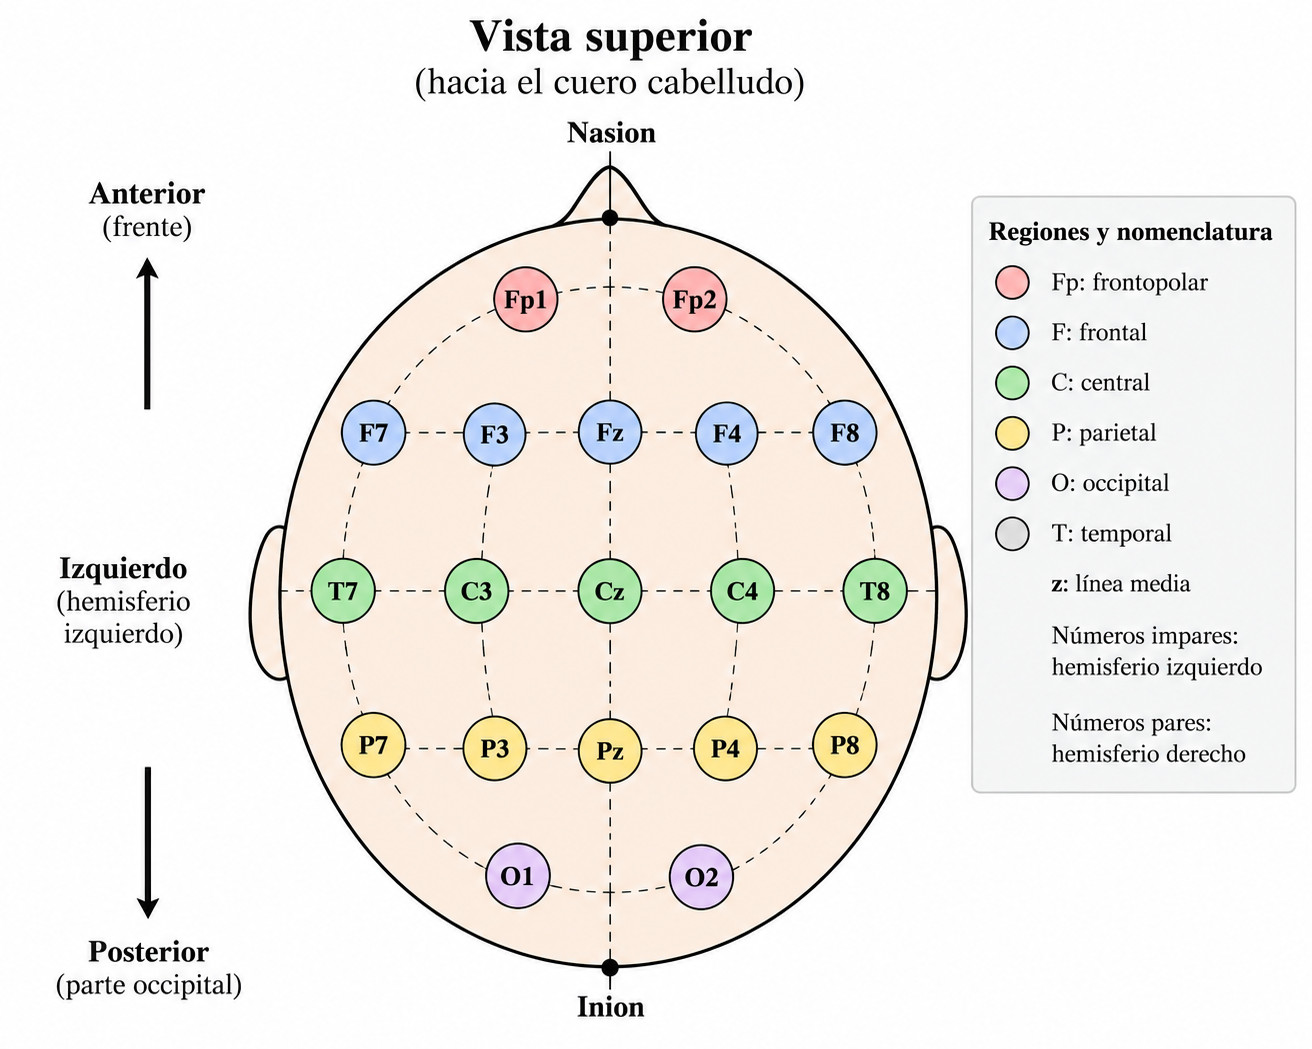
\includegraphics[width=0.90\textwidth]{ThesisFigs/sistema_10_20.png}
    \caption{Distribución de electrodos según el Sistema Internacional 10-20.
    Elaboración propia basada en \citet{StLouisFrey2016EEG} y
    \citet{Acharya2016ElectrodeNomenclature}.}
    \label{fig:sistema-10-20}
\end{figure}

La utilización de posiciones estandarizadas facilita la comparación de la
actividad registrada entre diferentes regiones y proporciona una referencia
común para la construcción de los canales EEG. Asimismo, permite establecer
configuraciones reproducibles para la presentación de las señales durante
su revisión. A partir de las relaciones establecidas entre estos electrodos
se construyen diferentes montajes electroencefalográficos, los cuales se
desarrollan en la siguiente subsección
\citep{Acharya2016ElectrodeNomenclature}.


\subsection{Montajes electroencefalográficos}
\label{subsec:montajes-eeg}

Un montaje electroencefalográfico corresponde a la organización de los
canales utilizados para presentar simultáneamente las señales de un registro
EEG. A partir de un mismo conjunto de electrodos pueden establecerse
diferentes relaciones entre sus señales, permitiendo visualizar la actividad
eléctrica cerebral desde distintas configuraciones sin modificar el registro
original. La selección del montaje constituye, por tanto, un elemento
importante durante la revisión e interpretación del EEG
\citep{StLouisFrey2016EEG,Acharya2016Montages}.

Los montajes pueden organizarse principalmente en configuraciones bipolares
y referenciales. En un montaje bipolar, cada canal representa la diferencia
de potencial entre dos electrodos del cuero cabelludo y los electrodos
adyacentes pueden disponerse formando secuencias o cadenas. En este tipo de
representación, un mismo electrodo puede participar en canales consecutivos,
lo que permite comparar la actividad entre regiones vecinas y contribuir a
la localización de determinadas formas de onda
\citep{Acharya2016Montages}.

Una configuración ampliamente utilizada es el montaje bipolar longitudinal,
en el cual los electrodos se relacionan siguiendo cadenas orientadas
principalmente en sentido anteroposterior. Este tipo de montaje es conocido
también de manera habitual como montaje de ``doble banana'', debido a la
disposición de las cadenas de derivaciones sobre ambos hemisferios. Ejemplos
de canales que pueden formar parte de estas cadenas son Fp1--F7, F7--T7,
T7--P7 y P7--O1 para el lado izquierdo, con relaciones correspondientes en
el lado derecho. Esta disposición permite observar cambios de polaridad entre
canales adyacentes y constituye una configuración de uso frecuente durante
la revisión de registros EEG
\citep{StLouisFrey2016EEG,Acharya2016Montages}.

En el montaje bipolar transversal, las relaciones entre electrodos se
organizan siguiendo cadenas orientadas predominantemente de manera
transversal respecto del eje anteroposterior de la cabeza. Esta configuración
proporciona una perspectiva diferente de la distribución espacial de la
actividad y complementa la información obtenida mediante los montajes
longitudinales. La utilización conjunta de distintas orientaciones puede
facilitar la evaluación de la localización y extensión de determinadas
formas de onda
\citep{Acharya2016Montages}.

En los montajes referenciales, cada electrodo activo se compara con una
referencia común. Como consecuencia, los diferentes canales comparten la
misma referencia y representan la diferencia de potencial entre cada
electrodo y dicha referencia. Dependiendo de la configuración empleada,
pueden utilizarse diferentes referencias, incluidas referencias derivadas
de combinaciones de electrodos. Una de las posibilidades utilizadas en los
sistemas digitales es la referencia promedio, obtenida a partir de la
información proporcionada por un conjunto de electrodos
\citep{StLouisFrey2016EEG,Acharya2016Montages}.

Los montajes bipolares y referenciales ofrecen representaciones
complementarias del mismo registro. La elección de una configuración puede
hacer que determinadas características de las señales resulten más evidentes
que en otra, por lo que la interpretación del EEG no debería depender
exclusivamente de una única disposición de canales. Las recomendaciones de la \textit{American Clinical Neurophysiology Society} (ACNS) contemplan el empleo de montajes bipolares y referenciales durante la interpretación clínica del EEG
\citep{Acharya2016Montages}.


En los sistemas digitales, la posibilidad de reorganizar las relaciones
entre las señales almacenadas permite representar un mismo registro
mediante diferentes montajes durante su revisión. La selección de
configuraciones bipolares longitudinales, transversales o referenciales
facilita que el profesional examine la distribución espacial de la
actividad eléctrica cerebral desde distintas perspectivas. El cambio
de montaje modifica la construcción y presentación de los canales,
sin alterar las señales originales ni requerir una nueva adquisición.


\subsection{Filtros y parámetros de visualización}
\label{subsec:filtros-parametros-eeg}

La visualización de un registro EEG requiere considerar diferentes parámetros
que determinan la forma en que las señales son presentadas al profesional.
En los sistemas digitales, algunos de estos parámetros pueden modificarse
durante la revisión del estudio sin alterar las señales originales
almacenadas. Entre ellos se encuentran los filtros de frecuencia, la
sensibilidad de visualización y la cantidad de tiempo representada en
pantalla \citep{StLouisFrey2016EEG,Sinha2016EEGTechnical}.

Los filtros permiten atenuar determinados componentes de frecuencia presentes
en la señal. El filtro de baja frecuencia, también denominado filtro pasa-altos,
atenúa los componentes de frecuencia inferiores a su frecuencia
de corte. Por su parte, el filtro de alta frecuencia o pasa-bajos
atenúa los componentes superiores a su frecuencia de corte. Asimismo, puede utilizarse un filtro de rechazo de banda
(\textit{notch}) para reducir la interferencia eléctrica concentrada alrededor
de una frecuencia determinada \citep{StLouisFrey2016EEG}.

La selección de los filtros debe realizarse con precaución, debido a que sus
ajustes pueden modificar la apariencia de las formas de onda. Un filtrado
excesivo puede atenuar componentes relevantes del registro o producir
distorsiones que dificulten su interpretación. Por este motivo, las
recomendaciones técnicas para EEG clínico establecen criterios para el uso de
los filtros y señalan la importancia de conservar adecuadamente la información
contenida en las diferentes bandas de frecuencia
\citep{Sinha2016EEGTechnical}.

Otro parámetro importante es la sensibilidad, que determina la escala vertical
con la que se representan las variaciones de voltaje del EEG. En la
representación convencional se expresa como la relación entre una determinada
amplitud de entrada, medida en microvoltios, y la deflexión producida en la
visualización. La modificación de la sensibilidad permite aumentar o reducir
la altura con la que aparecen las formas de onda, facilitando la inspección de
señales de diferentes amplitudes sin modificar los valores originales del
registro \citep{StLouisFrey2016EEG,Sinha2016EEGTechnical}.

La escala temporal constituye igualmente un elemento relevante durante la
revisión del EEG. En los sistemas digitales puede modificarse la cantidad de
tiempo representada dentro del área de visualización. Mostrar un intervalo
temporal menor permite observar con mayor separación horizontal los cambios
que ocurren en las señales, mientras que una ventana temporal mayor permite
examinar una porción más extensa del registro dentro de la misma pantalla.
La elección de este parámetro depende de las características que el
profesional desea analizar durante la revisión.

La posibilidad de modificar filtros, sensibilidad y escala temporal durante
la revisión constituye una de las ventajas de los sistemas EEG digitales.
Estos controles proporcionan diferentes formas de presentar un mismo registro
y pueden facilitar la identificación y evaluación visual de determinadas
características de las señales. No obstante, su utilización debe considerar
que los ajustes de visualización y filtrado pueden influir en la apariencia
del trazado y, por tanto, deben ser interpretados adecuadamente por el
profesional \citep{StLouisFrey2016EEG,Sinha2016EEGTechnical}.


\section{Representación y procesamiento de señales EEG}
\label{sec:representacion-procesamiento-eeg}

La adquisición de un EEG produce un conjunto de señales digitales que
representan la evolución de la actividad eléctrica registrada a lo largo del
tiempo. Para que estas señales puedan ser almacenadas, intercambiadas,
visualizadas y posteriormente procesadas mediante herramientas informáticas,
es necesario disponer de estructuras que permitan conservar tanto las
muestras obtenidas como la información necesaria para interpretarlas
correctamente.

La representación digital de un registro EEG comprende, además de los valores
correspondientes a las muestras de las señales, información relacionada con
los canales registrados, sus unidades físicas, la frecuencia de muestreo y
otros parámetros asociados con la adquisición. La conservación de estos
elementos permite que un registro pueda ser posteriormente reconstruido y
presentado mediante diferentes herramientas de visualización y análisis.

El empleo de formatos documentados para almacenar señales fisiológicas
facilita además el intercambio de registros entre diferentes sistemas. Uno
de los formatos utilizados ampliamente para este propósito en el ámbito de
la electroencefalografía es el \textit{European Data Format} (EDF), diseñado
para el almacenamiento e intercambio de registros fisiológicos digitalizados
\citep{Kemp1992EDF}.

\subsection{Estándar EDF}
\label{subsec:estandar-edf}

El \textit{European Data Format} (EDF) es un formato desarrollado para
facilitar el intercambio y almacenamiento de registros fisiológicos
digitalizados. Fue presentado por Kemp y colaboradores en 1992 con el
propósito de proporcionar una estructura sencilla que pudiera utilizarse
independientemente de plataformas específicas de \textit{hardware} o \textit{software}. El formato permite almacenar múltiples señales dentro de un mismo archivo y admite que estas posean características de adquisición diferentes
\citep{Kemp1992EDF}.

Un archivo EDF se organiza principalmente en un registro de cabecera y una
serie de registros de datos. La cabecera contiene información general sobre
el registro y describe las características técnicas de las señales
almacenadas. Entre los datos incluidos se encuentran la identificación del
registro, la fecha y hora de inicio, el número de señales y la duración de
los registros de datos. Para cada señal se almacenan además elementos como
su etiqueta, unidad física, valores mínimos y máximos físicos y digitales,
información de prefiltrado y cantidad de muestras por registro
\citep{Kemp1992EDF}.

Después de la cabecera se encuentran los registros de datos, que contienen
las muestras digitalizadas correspondientes a las diferentes señales. Estos
registros representan intervalos consecutivos de duración determinada y
organizan las muestras de cada señal de acuerdo con la información
especificada en la cabecera. Debido a que cada señal posee su propia cantidad
de muestras por registro, el formato permite almacenar dentro de un mismo
archivo señales adquiridas con diferentes frecuencias de muestreo
\citep{Kemp1992EDF}.

La relación entre los valores digitales almacenados y las magnitudes físicas
de las señales se establece mediante los valores mínimos y máximos definidos
para cada canal. De esta manera, las muestras digitales pueden convertirse
en valores expresados en la unidad física correspondiente, como microvoltios
en el caso de las señales EEG. Esta información resulta necesaria para
reconstruir adecuadamente la amplitud de las señales durante su posterior
visualización o procesamiento.

Una característica relevante del formato es que la información necesaria
para interpretar cada señal se encuentra asociada al propio registro. 
Las etiquetas de los canales, las unidades físicas, la calibración y otros
parámetros permiten que aplicaciones compatibles puedan recuperar las
señales y representarlas posteriormente. Asimismo, los parámetros de
visualización, como los montajes o determinados ajustes de presentación,
pueden modificarse durante la revisión digital sin alterar las muestras
originales almacenadas \citep{StLouisFrey2016EEG}.


Posteriormente se desarrolló EDF+, una extensión compatible con EDF que
incorporó nuevas posibilidades para el almacenamiento de registros
fisiológicos, entre ellas el manejo de registros interrumpidos y la
incorporación de anotaciones asociadas temporalmente con el registro. Estas
características ampliaron las posibilidades del formato para representar
eventos y otra información relacionada con estudios neurofisiológicos \citep{KempOlivan2003EDFPlus}.



\subsection{Espectrograma}
\label{subsec:espectrograma}

La representación convencional de una señal EEG permite observar cómo varía
su amplitud a lo largo del tiempo. Sin embargo, las señales
electroencefalográficas están compuestas por actividad correspondiente a
diferentes frecuencias, cuyo comportamiento también puede variar durante el
registro. El análisis espectral permite estudiar este contenido frecuencial
y constituye una herramienta complementaria para caracterizar las señales
EEG.

Una representación únicamente en el dominio de la frecuencia permite conocer
la distribución de los componentes frecuenciales presentes en una señal,
pero no necesariamente permite determinar en qué momento aparecen o cambian
dichos componentes. Debido a que la actividad EEG puede presentar variaciones
a lo largo del tiempo, resulta útil emplear representaciones que conserven
simultáneamente información temporal y frecuencial
\citep{Ng2022EEGSpectrograms}.

El espectrograma es una representación tiempo--frecuencia que permite
visualizar cómo evoluciona el contenido frecuencial de una señal durante un
intervalo determinado. Habitualmente, el tiempo se representa sobre el eje
horizontal y la frecuencia sobre el eje vertical, mientras que la potencia
asociada a cada combinación de tiempo y frecuencia se representa mediante
una escala de colores. De esta manera, el espectrograma proporciona una
representación visual de los cambios en la distribución de potencia de las
diferentes frecuencias a lo largo del registro
\citep{Ng2022EEGSpectrograms}.

Una forma de obtener esta representación consiste en dividir la señal en
segmentos temporales y calcular sucesivamente su contenido frecuencial.
La Transformada de Fourier de Tiempo Corto (\textit{Short-Time Fourier
Transform}, STFT) aplica este principio mediante ventanas temporales
que se desplazan sucesivamente a lo largo de la señal. Los espectros calculados para las sucesivas ventanas pueden organizarse en función del tiempo para construir el espectrograma. Este procedimiento permite conservar información sobre cuándo se presentan los diferentes componentes frecuenciales, a diferencia de un análisis espectral realizado sobre el registro completo \citep{Ng2022EEGSpectrograms}.

La utilización de ventanas temporales implica un compromiso entre la
resolución temporal y la resolución frecuencial de la representación.
Ventanas de menor duración permiten localizar con mayor precisión cambios
en el tiempo, mientras que ventanas de mayor duración proporcionan una mejor
resolución para distinguir componentes próximos en frecuencia. Por este
motivo, los parámetros empleados para generar un espectrograma influyen en
la forma en que la información de la señal es representada \citep{Ng2022EEGSpectrograms}.

En el análisis de registros EEG, el espectrograma permite condensar
información correspondiente a períodos extensos y facilitar la observación
de cambios en el contenido frecuencial de las señales. Determinados patrones
pueden producir modificaciones en la distribución de potencia y aparecer
como estructuras diferenciadas dentro de la representación
tiempo--frecuencia. No obstante, el espectrograma constituye una
representación derivada de las señales EEG y su interpretación debe
relacionarse con el registro electroencefalográfico original
\citep{Ng2022EEGSpectrograms}.




\section{Análisis de señales EEG aplicado a la epilepsia}
\label{sec:analisis-eeg-epilepsia}


El análisis del EEG constituye una herramienta complementaria
importante en la evaluación de pacientes con sospecha o
diagnóstico de epilepsia.Su utilidad se basa en la posibilidad de observar características de la actividad eléctrica cerebral que, interpretadas conjuntamente con la información clínica del paciente, pueden aportar elementos para apoyar el diagnóstico, la clasificación de las crisis y la caracterización de
determinados síndromes epilépticos. No obstante, la interpretación del EEG
debe realizarse dentro del contexto clínico y sus hallazgos no deben
considerarse de manera aislada \citep{NoachtarRemi2009}.

Durante la revisión de un registro pueden distinguirse, entre otros, períodos
ictales e interictales. El período ictal se encuentra relacionado con la
ocurrencia de una crisis epiléptica y puede presentar patrones
electroencefalográficos que evolucionan en el tiempo. El período interictal,
en cambio, corresponde al intervalo entre las crisis, durante el cual pueden
observarse determinadas alteraciones de interés para la evaluación de la
epilepsia. Entre ellas se encuentran las descargas epileptiformes
interictales, conocidas por sus siglas en inglés como IED
(\textit{interictal epileptiform discharges})
\citep{NoachtarRemi2009}.

Las descargas epileptiformes interictales corresponden a patrones
electroencefalográficos transitorios que presentan características
morfológicas y espaciales que permiten diferenciarlos de la actividad de
fondo. Su reconocimiento requiere considerar distintos atributos de la forma
de onda y de su distribución sobre el cuero cabelludo. La \textit{International Federation of Clinical Neurophysiology} (IFCN) ha propuesto criterios operacionales para contribuir a una identificación más sistemática de estas
descargas, considerando características como la morfología, la duración
respecto de la actividad de fondo, la asimetría de la forma de onda, la
presencia de una onda lenta posterior, la alteración de la actividad de fondo
y la distribución espacial de los potenciales
\citep{Kural2020IEDCriteria}.

La identificación de actividad epileptiforme requiere especial cuidado debido
a que determinados transitorios fisiológicos, artefactos u otras formas de
onda pueden presentar características que conduzcan a interpretaciones
incorrectas. La sobreinterpretación de hallazgos electroencefalográficos
puede contribuir a una clasificación errónea de determinadas formas de onda
como epileptiformes. Por esta razón, el análisis visual realizado por
profesionales con experiencia y la utilización de criterios definidos
continúan siendo elementos relevantes durante la interpretación del EEG
\citep{Kural2020IEDCriteria}.

Además de reconocer la morfología de una determinada forma de onda, durante
el análisis resulta relevante examinar su distribución espacial y temporal.
La comparación entre canales y montajes puede aportar información sobre las
regiones en las que una actividad presenta mayor expresión, mientras que la
observación de su evolución temporal permite analizar cómo se desarrolla a
lo largo del registro. Los montajes, filtros, parámetros de visualización y
otras representaciones complementarias pueden facilitar esta revisión, pero
su utilización debe mantenerse vinculada con la interpretación del trazado
electroencefalográfico original \citep{NoachtarRemi2009,StLouisFrey2016EEG}.

El análisis de registros prolongados puede implicar la revisión de una gran
cantidad de señales correspondientes a numerosos canales y extensos períodos
de tiempo. En este contexto, las herramientas informáticas pueden contribuir
a organizar la información y asistir al profesional durante la exploración
del estudio. Los métodos automatizados pueden utilizarse para señalar
segmentos o patrones potencialmente relevantes que posteriormente sean
revisados por el especialista, sin que dicha detección sustituya la
interpretación clínica del registro.

La combinación de visualización electroencefalográfica y procesamiento
automatizado puede facilitar la localización de segmentos potencialmente
relevantes para su revisión posterior. La valoración de estos hallazgos
y su relación con el contexto clínico corresponden al especialista.



\section{Inteligencia artificial aplicada al análisis de EEG}
\label{sec:ia-analisis-eeg}

El análisis de señales EEG puede requerir la revisión de grandes cantidades
de información obtenida a partir de múltiples canales y durante períodos
prolongados. Además, las características de estas señales pueden variar entre
pacientes y a lo largo de un mismo registro. En este contexto, las técnicas
de inteligencia artificial han sido investigadas como herramientas para
procesar automáticamente señales electroencefalográficas e identificar
características o patrones de interés que puedan complementar su revisión
\citep{Ahmad2022EEGMachineLearning}.


Entre las técnicas de inteligencia artificial aplicadas al EEG se
encuentran el aprendizaje automático y el aprendizaje profundo.
Estos enfoques han sido investigados para tareas como la detección,
clasificación y predicción de crisis epilépticas. Algunos métodos
utilizan características obtenidas previamente mediante técnicas
de procesamiento de señales, mientras que otros emplean
arquitecturas capaces de aprender representaciones directamente
a partir de los datos \citep{Ahmad2022EEGMachineLearning}.


De manera general, un sistema automatizado para el análisis de EEG puede
comprender diferentes etapas, como la preparación de las señales, su
segmentación, la obtención o aprendizaje de características y la aplicación
de un modelo para generar una clasificación o resultado. Las características
consideradas pueden estar relacionadas con propiedades temporales,
frecuenciales o tiempo--frecuencia de las señales, entre otras
representaciones utilizadas para distinguir determinados patrones
electroencefalográficos \citep{Ahmad2022EEGMachineLearning}.

El aprendizaje profundo (\textit{deep learning}) constituye un conjunto de
técnicas dentro del aprendizaje automático que utiliza modelos con múltiples
niveles de representación. A diferencia de enfoques tradicionales que pueden
depender en mayor medida de características definidas previamente, estos
modelos pueden aprender representaciones relevantes a partir de los datos
utilizados durante su entrenamiento. Diferentes arquitecturas de aprendizaje
profundo han sido estudiadas para tareas relacionadas con la detección y
clasificación de crisis a partir de señales EEG
\citep{Ahmad2022EEGMachineLearning}.

Sin embargo, el desempeño obtenido por un modelo depende de diversos factores,
entre ellos las características de los datos utilizados, las etapas de
preprocesamiento, la variabilidad entre pacientes y las condiciones en las
que se adquieren las señales. El EEG presenta además características
no estacionarias y puede contener artefactos o interferencias que dificultan
su procesamiento automático. Por estas razones, los resultados obtenidos en
conjuntos de datos específicos no implican necesariamente un comportamiento
equivalente en otros pacientes o entornos clínicos
\citep{Ahmad2022EEGMachineLearning}.

La utilización de inteligencia artificial en este ámbito debe entenderse,
por tanto, como una herramienta potencial de apoyo al análisis y no como un
reemplazo automático de la interpretación realizada por el profesional. Los
resultados generados por estos métodos requieren ser considerados dentro del
contexto del registro y de la información clínica disponible, especialmente
cuando forman parte de procesos relacionados con la evaluación de pacientes
con epilepsia \citep{Ahmad2022EEGMachineLearning}.

\subsection{Aprendizaje automático aplicado a señales EEG}
\label{subsec:aprendizaje-automatico-eeg}

El aprendizaje automático (\textit{machine learning}) comprende un conjunto de
métodos computacionales capaces de identificar patrones a partir de datos y
utilizarlos posteriormente para realizar tareas como clasificación, detección
o predicción. En el ámbito del análisis de señales EEG, estas técnicas permiten
procesar información obtenida de la actividad eléctrica cerebral con el
propósito de reconocer características asociadas con determinados estados o
eventos de interés \citep{Rasheed2021MachineLearning}.

La aplicación de técnicas de aprendizaje automático sobre señales EEG
generalmente requiere una serie de etapas de procesamiento. En un enfoque
tradicional, el registro puede dividirse en segmentos o ventanas temporales,
sobre los cuales se calculan características que representan determinados
aspectos de la señal. Estas características pueden obtenerse a partir del
dominio temporal, frecuencial o de otras representaciones de la señal, y
posteriormente son utilizadas como entrada de un algoritmo de clasificación
\citep{Rasheed2021MachineLearning}.

Este proceso puede representarse conceptualmente mediante una secuencia
compuesta por la adquisición de la señal EEG, su preprocesamiento y
segmentación, la extracción de características y, finalmente, la aplicación
de un modelo encargado de generar una salida. Dependiendo del objetivo del
sistema, dicha salida puede corresponder, por ejemplo, a la identificación de
un segmento como perteneciente o no a una determinada categoría. La calidad
de los datos utilizados y la selección de características relevantes influyen
en el desempeño de los métodos tradicionales de aprendizaje automático.

En el aprendizaje supervisado, los modelos se construyen utilizando ejemplos
para los cuales se dispone previamente de una etiqueta o categoría conocida.
Durante el entrenamiento, el algoritmo utiliza estos ejemplos para aprender
relaciones entre las características de entrada y las clases correspondientes.
Una vez construido el modelo, este puede aplicarse sobre nuevos datos para
obtener una clasificación o estimación. Para valorar su capacidad de generalización, resulta necesario separar los datos utilizados durante el entrenamiento de aquellos destinados a la validación y evaluación del modelo,
evitando que los mismos ejemplos se utilicen para entrenarlo y medir posteriormente su desempeño \citep{Rasheed2021MachineLearning}.

Además de los métodos tradicionales, el desarrollo del aprendizaje profundo
(\textit{deep learning}) ha permitido aplicar modelos capaces de aprender
representaciones de los datos con una menor dependencia de características
definidas manualmente. Arquitecturas como las redes neuronales convolucionales
y las redes neuronales recurrentes han sido estudiadas en diferentes tareas
de clasificación de EEG debido a su capacidad para modelar patrones presentes
en señales complejas y datos con estructura temporal
\citep{Craik2019DeepLearning}.

La aplicación de aprendizaje automático a señales EEG presenta, sin embargo,
diversos desafíos. Los registros pueden contener artefactos y ruido, además de
presentar variaciones entre pacientes, sesiones de registro y condiciones de
adquisición. Asimismo, la disponibilidad y calidad de los datos etiquetados
condicionan el entrenamiento y la evaluación de los modelos. Por estas
razones, un desempeño favorable sobre un conjunto de datos determinado no
implica necesariamente que el modelo mantenga el mismo comportamiento sobre
registros obtenidos en condiciones diferentes
\citep{Rasheed2021MachineLearning}.

En el contexto de la epilepsia, estas técnicas han sido investigadas para
analizar registros EEG y asistir en tareas relacionadas con la identificación
de patrones de interés, incluyendo la detección y predicción de crisis
epilépticas. El resultado producido por un modelo puede utilizarse para
señalar determinados segmentos del registro y facilitar su posterior revisión.
La detección automatizada de crisis y anomalías electroencefalográficas se
aborda con mayor detalle en la siguiente sección.

\subsection{Detección automatizada de crisis y anomalías}
\label{subsec:deteccion-automatizada-crisis-anomalias}

La detección automatizada aplicada al EEG tiene como propósito identificar
segmentos del registro que presentan características compatibles con
determinados patrones de interés. En el ámbito de la epilepsia, una de las
aplicaciones más estudiadas corresponde a la detección de crisis epilépticas,
aunque también se han desarrollado métodos orientados a reconocer otras
alteraciones electroencefalográficas, como las descargas epileptiformes
interictales. Estas tareas no son equivalentes, debido a que representan
fenómenos diferentes dentro del registro EEG
\citep{NoachtarRemi2009,Kural2020IEDCriteria}.

En los sistemas de detección automatizada, el registro EEG puede dividirse
en segmentos o ventanas temporales que son analizados individualmente por un
modelo. A partir de las características presentes en cada segmento, el sistema
puede generar una clasificación o una estimación asociada con la presencia de
un patrón determinado. Posteriormente, los resultados correspondientes a
segmentos consecutivos pueden ser considerados dentro de su contexto temporal
para identificar períodos del registro que requieren una revisión más
detallada \citep{Rasheed2021MachineLearning}.

La detección de una crisis implica reconocer actividad electroencefalográfica
compatible con un evento ictal y localizar temporalmente su ocurrencia dentro
del registro. Por su parte, la detección de descargas epileptiformes
interictales se orienta a identificar patrones que aparecen entre las crisis
y que pueden aportar información relevante para la evaluación del EEG. La
morfología, duración, distribución espacial y relación con la actividad de
fondo son algunos de los elementos considerados durante la interpretación de
estas descargas \citep{Kural2020IEDCriteria}.

El desempeño de un método de detección no debe valorarse únicamente por la
cantidad de eventos que logra identificar. También resulta necesario
considerar las detecciones incorrectas producidas durante el análisis.
En este contexto, la sensibilidad expresa la proporción de eventos
de interés correctamente identificados respecto del total de
eventos de interés presentes en los datos. Por su parte, los
falsos positivos corresponden a detecciones realizadas por el
sistema que no representan el evento buscado. En registros prolongados, la cantidad de falsas alarmas por unidad de tiempo constituye también una medida relevante para evaluar la utilidad práctica de un detector
\citep{Rasheed2021MachineLearning}.

La existencia de falsos positivos y falsos negativos constituye uno de los
principales desafíos de estos sistemas. Artefactos producidos por movimientos,
actividad muscular, interferencias eléctricas u otros componentes de la señal
pueden presentar características que dificultan la clasificación automática.
Además, las manifestaciones electroencefalográficas de las crisis pueden
variar entre pacientes y entre diferentes episodios de un mismo paciente,
lo que dificulta la generalización de los modelos a registros distintos de
aquellos utilizados durante su desarrollo
\citep{Rasheed2021MachineLearning}.


Por estas razones, los resultados obtenidos mediante detección
automatizada deben considerarse elementos de apoyo para la
revisión del registro EEG. Un sistema puede señalar segmentos
potencialmente relevantes y facilitar su localización dentro
de registros extensos, pero la interpretación de estos hallazgos
debe realizarse considerando las señales originales y el
contexto clínico del paciente. De esta manera, la automatización
puede contribuir a priorizar segmentos para su revisión, sin
sustituir la valoración realizada por el profesional especialista.


\section{Sistemas y herramientas para gestión y visualización de EEG}
\label{sec:sistemas-herramientas-eeg}

El registro y análisis de señales EEG se apoya en sistemas especializados que
integran diferentes funciones relacionadas con la adquisición, almacenamiento,
visualización y revisión de los estudios electroencefalográficos. Estas
soluciones pueden incorporar herramientas para configurar montajes, modificar
parámetros de visualización, navegar temporalmente por los registros, asociar
vídeo a las señales y elaborar informes derivados de los estudios.

Las características disponibles dependen del propósito y de la arquitectura
de cada solución. Algunos sistemas forman parte de plataformas
neurodiagnósticas asociadas a equipos específicos de adquisición, mientras
que otras herramientas se orientan al procesamiento, visualización o análisis
posterior de señales EEG. Asimismo, existen soluciones que incorporan
funciones de acceso remoto, gestión de datos y procesamiento automatizado como
apoyo a la revisión de los registros.

A continuación, se describen algunas herramientas relacionadas con el
contexto de este trabajo. Se considera en primer lugar Easy III de Cadwell,
utilizado en el entorno donde se desarrolla el proyecto; posteriormente se
presenta EEG Trend Software de Nihon Kohden y, finalmente, se revisan
plataformas web y otras herramientas relacionadas con la visualización y el
análisis de señales EEG.


\subsection{Easy Cadwell III}
\label{subsec:easy-cadwell-iii}

Easy III EEG es una solución desarrollada por Cadwell para la adquisición,
monitorización y revisión de estudios electroencefalográficos. El sistema está
orientado a diferentes escenarios de utilización del EEG, incluyendo estudios
clínicos, monitorización prolongada y monitorización continua. La plataforma
combina componentes de adquisición con herramientas de \textit{software} destinadas a la visualización y gestión de los registros \citep{CadwellEasyIII}.

Entre sus funcionalidades se encuentran la configuración de la interfaz de
usuario, la utilización y modificación de montajes, la revisión temporal de
los registros y la integración de vídeo con los estudios EEG. El sistema
también dispone de funciones relacionadas con la gestión del flujo de trabajo,
almacenamiento de información clínica, generación de informes y registro de
accesos de los usuarios \citep{CadwellEasyIII}.


Durante la revisión de un estudio, el \textit{software} permite recorrer
los datos por páginas, segundos, comentarios o eventos, modificar la
velocidad de revisión y realizar cambios de montaje. Estas funciones facilitan la exploración de registros prolongados y la observación de las señales desde diferentes configuraciones de visualización \citep{CadwellEasyIIISpecifications}.

En el Hospital Central del Instituto de Previsión Social, Easy III
forma parte de las herramientas empleadas para el trabajo con estudios EEG.
Su utilización constituye un ejemplo de integración de adquisición,
visualización y revisión de registros en un entorno clínico.

\begin{figure}[htbp]
    \centering

    \begin{minipage}[c]{0.45\textwidth}
        \centering
        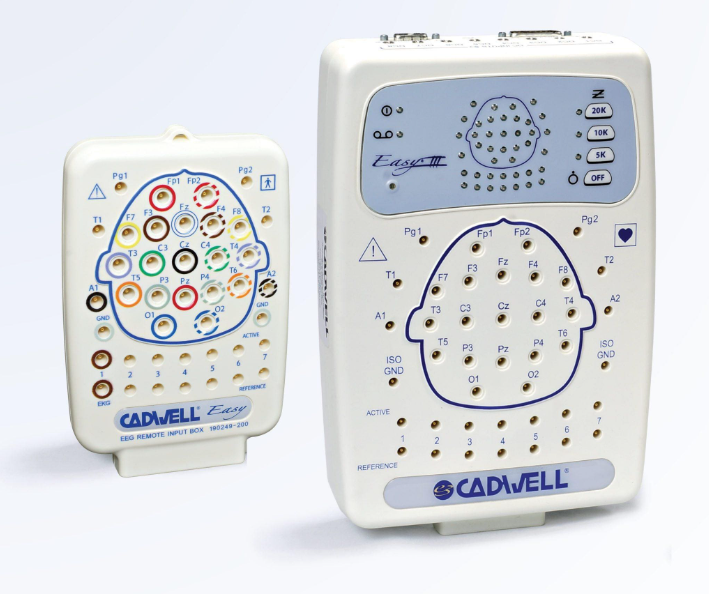
\includegraphics[
            width=\linewidth,
            height=5cm,
            keepaspectratio
        ]{Chapter2/Chapter2Figs/cadwell_modulos.png}

        \small (a) Módulos de adquisición EEG.
    \end{minipage}
    \hfill
    \begin{minipage}[c]{0.45\textwidth}
        \centering
        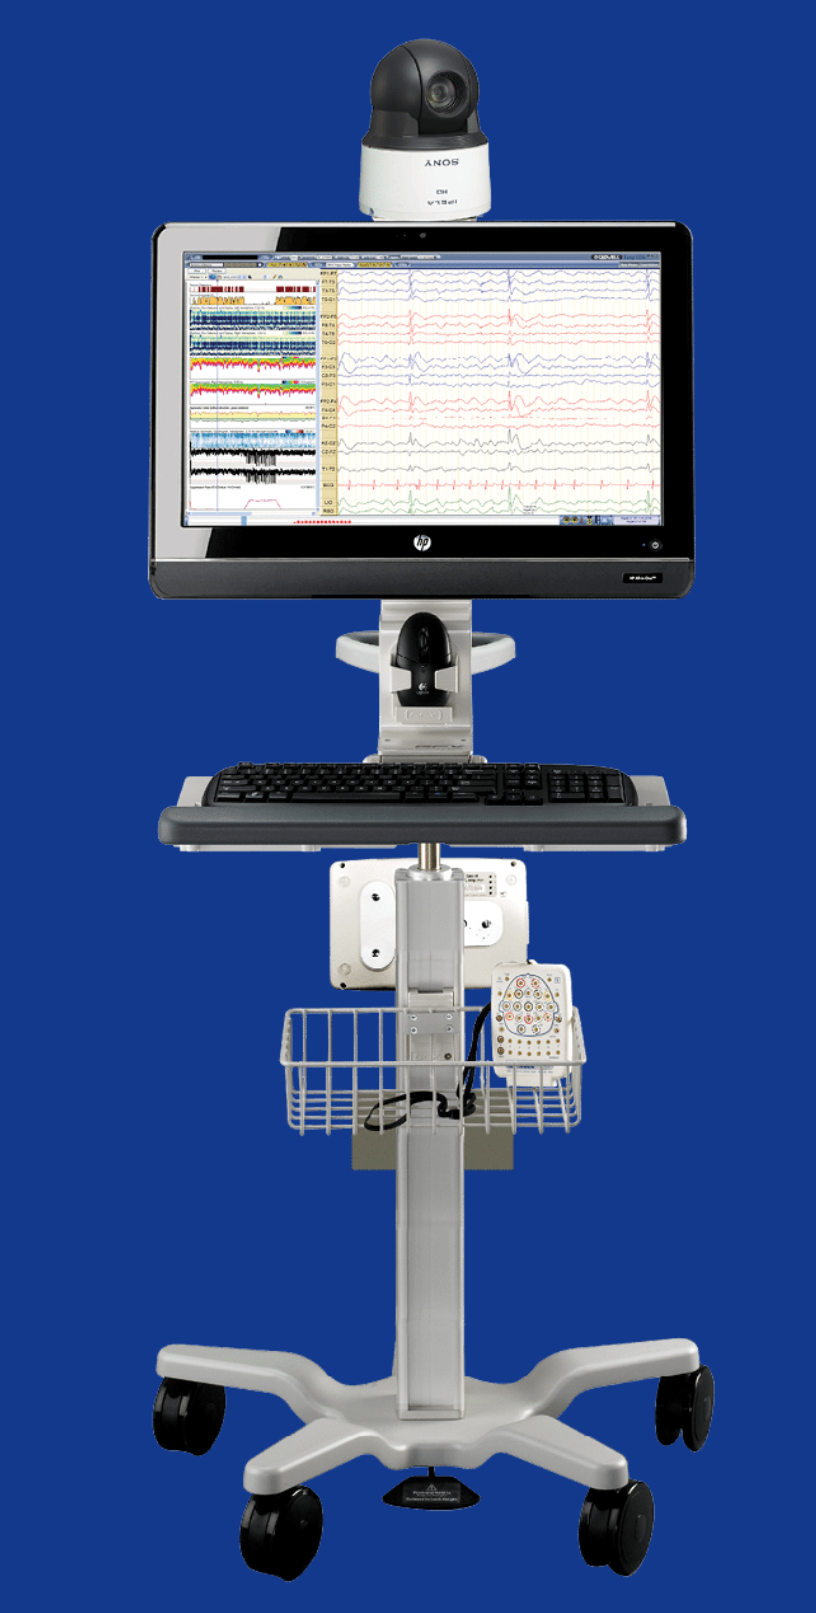
\includegraphics[
            width=\linewidth,
            height=5cm,
            keepaspectratio
        ]{Chapter2/Chapter2Figs/cadwell_estacion.png}

        \small (b) Estación de trabajo EEG.
    \end{minipage}

    \caption{Componentes del sistema Easy III EEG de Cadwell:
    (a) módulos de adquisición de señales y
    (b) estación de trabajo para visualización y revisión de EEG.
    Fuente: Cadwell Industries \citep{CadwellEasyIII}.}
    \label{fig:cadwell-easy-iii}
\end{figure}





\subsection{EEG Trend Software de Nihon Kohden}
\label{subsec:eeg-trend-nihon-kohden}

EEG Trend Software es una herramienta desarrollada por Nihon Kohden orientada
a la visualización y análisis de registros EEG, particularmente mediante el
uso de EEG cuantitativo y representaciones de tendencias. El \textit{software} permite observar cambios producidos a lo largo del tiempo y dispone de anotaciones
codificadas por colores y registros de eventos integrados como apoyo al
proceso de revisión \citep{NihonKohdenEEGTrend}.

La herramienta permite personalizar la disposición de las visualizaciones de
EEG y tendencias, así como comparar información correspondiente a diferentes
intervalos temporales. Los datos de registros prolongados pueden presentarse
mediante tendencias que condensan la información de varios días o incluso
semanas. Asimismo, el sistema dispone de herramientas de anotación y edición,
y contempla la utilización opcional de vídeo digital sincronizado para
contrastar las señales EEG con posibles artefactos observados durante el
registro \citep{NihonKohdenEEGTrend}.

Entre sus funciones de procesamiento se encuentra el análisis espectral de
las señales mediante la transformada rápida de Fourier (FFT). A partir de
este procesamiento, el \textit{software} puede presentar diferentes representaciones y parámetros, entre ellos arreglos espectrales de densidad (DSA), potencia, borde espectral y relaciones de potencia. También permite representar EEG integrado en amplitud (aEEG) y determinados parámetros relacionados con patrones de supresión de ráfagas \citep{NihonKohdenEEGTrend}.

EEG Trend Software incorpora además funciones orientadas a facilitar la
identificación de determinados eventos durante la revisión. De acuerdo con la documentación del fabricante, pueden utilizarse algoritmos opcionales de detección de crisis epilépticas en adultos y neonatos, los cuales señalan formas de onda que podrían corresponder a eventos electrográficos de interés para facilitar su posterior identificación y revisión. Asimismo, dispone de un mecanismo de detección de artefactos de electrodos que permite señalar tendencias que podrían estar influenciadas por dichos artefactos
\citep{NihonKohdenEEGTrend}.

Estas características muestran un enfoque en el que la visualización del EEG
puede complementarse mediante representaciones cuantitativas, análisis
espectral, tendencias y mecanismos automatizados de detección. La información
generada por estas herramientas puede facilitar la localización y revisión de
períodos de interés dentro de registros prolongados, manteniendo la señal EEG
como elemento fundamental para su interpretación.

\begin{figure}[htbp]
    \centering

    \begin{minipage}[c]{0.45\textwidth}
        \centering
        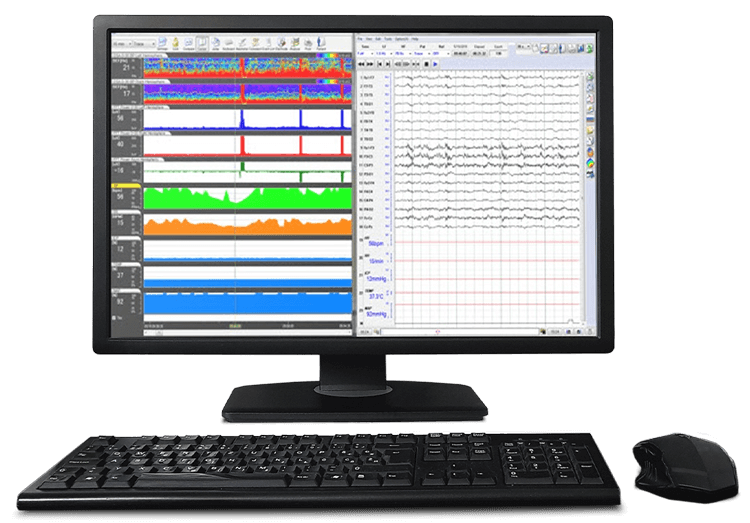
\includegraphics[
            width=\linewidth,
            height=5cm,
            keepaspectratio
        ]{Chapter2/Chapter2Figs/nihon_kohden_software.png}

        \small (a) Visualización de señales y tendencias EEG.
    \end{minipage}
    \hfill
    \begin{minipage}[c]{0.45\textwidth}
        \centering
        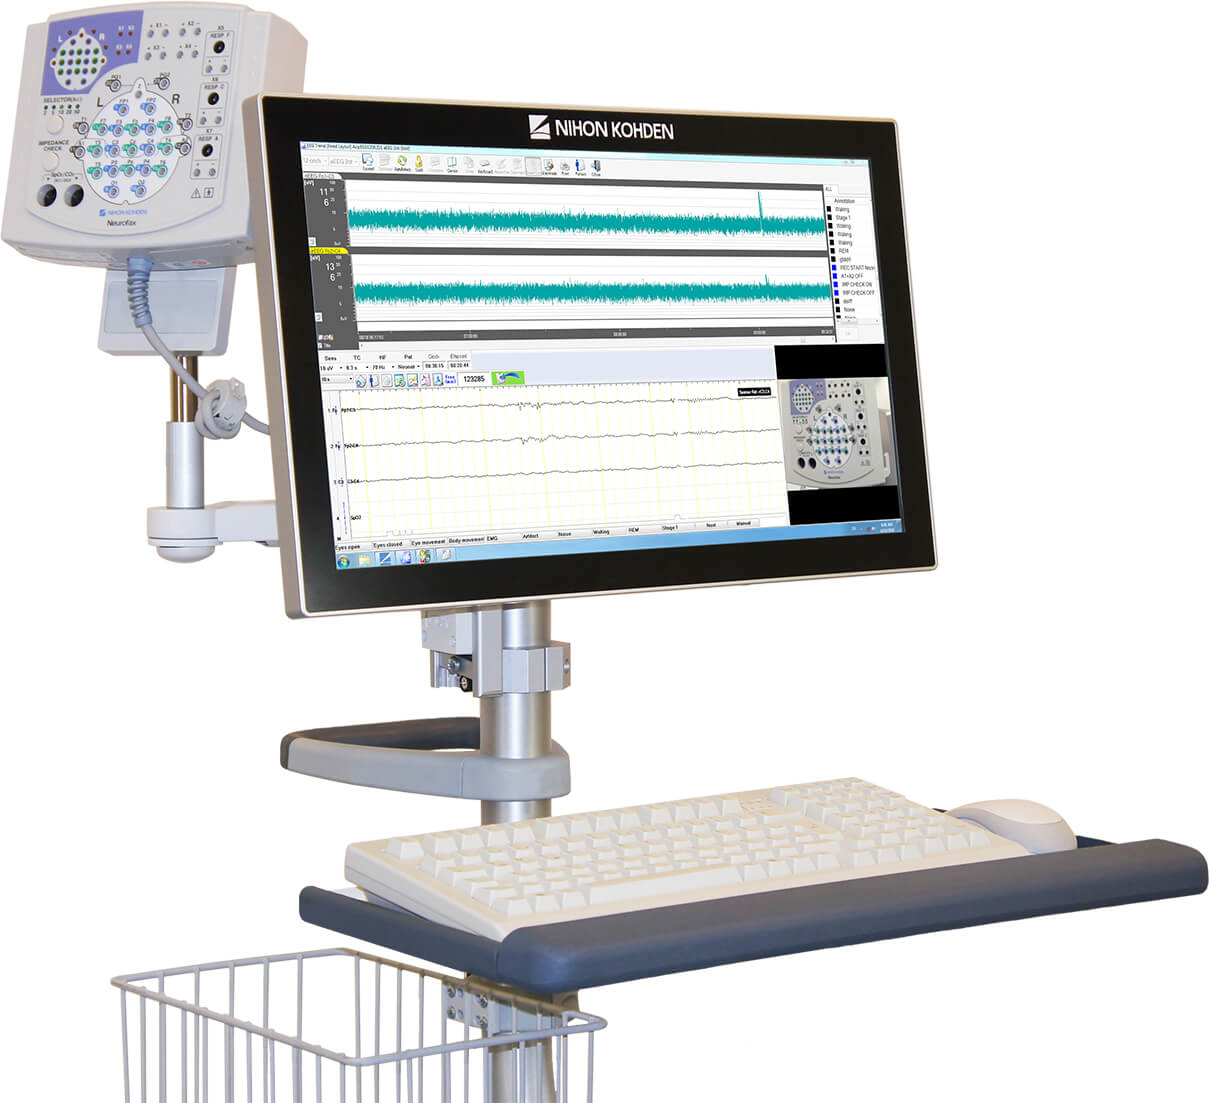
\includegraphics[
            width=\linewidth,
            height=5cm,
            keepaspectratio
        ]{Chapter2/Chapter2Figs/nihon_kohden_estacion.png}

        \small (b) Estación de trabajo EEG.
    \end{minipage}

    \caption{Herramientas de visualización y equipamiento EEG
    de Nihon Kohden: (a) interfaz de análisis de señales y
    tendencias y (b) estación de trabajo.
    Fuente: Nihon Kohden \citep{NihonKohdenEEGTrend}.}
    \label{fig:nihon-kohden-eeg-trend}
\end{figure}


\subsection{Plataformas web y herramientas relacionadas}
\label{subsec:plataformas-herramientas-eeg}

Además de los sistemas comerciales utilizados en entornos clínicos, existen
herramientas de código abierto destinadas al procesamiento, análisis y
visualización de señales EEG. Estas soluciones son utilizadas principalmente
en ámbitos de investigación y desarrollo, y proporcionan funcionalidades que
permiten trabajar con diferentes formatos de datos neurofisiológicos,
preprocesar señales, visualizar registros y aplicar distintos métodos de
análisis.

MNE-Python es una biblioteca de código abierto desarrollada en Python para el
procesamiento y análisis de datos neurofisiológicos, incluyendo señales EEG.
Esta biblioteca proporciona funcionalidades para la lectura de diferentes
formatos de datos, preprocesamiento, visualización de señales, análisis
tiempo--frecuencia, estimación de fuentes, conectividad, estadística y
aplicación de técnicas de aprendizaje automático
\citep{Gramfort2013MNE}.

Otra herramienta ampliamente utilizada es EEGLAB, un entorno de código abierto
desarrollado sobre MATLAB para el procesamiento de datos
electroencefalográficos. Permite importar y gestionar conjuntos de datos EEG,
visualizar señales y eventos, aplicar procedimientos de preprocesamiento y
realizar diferentes tipos de análisis. Su arquitectura admite además la
incorporación de extensiones mediante complementos desarrollados para tareas
específicas \citep{DelormeMakeig2004}.


Junto con estas herramientas, el desarrollo de tecnologías web ha permitido
la aparición de aplicaciones capaces de visualizar señales
electroencefalográficas mediante interfaces accesibles desde un navegador.
Entre los antecedentes se encuentra EpiCurrents, una herramienta orientada
a la visualización y revisión de señales neurofisiológicas en entornos web,
con funcionalidades para explorar registros electroencefalográficos
\citep{EpiCurrentsWebViewer}.
Este tipo de herramientas constituye un antecedente de la incorporación
de funcionalidades de revisión y análisis de señales EEG en entornos
interactivos basados en tecnologías web.


Las diferentes alternativas muestran que el análisis de EEG puede abordarse
mediante herramientas con propósitos y arquitecturas diversas. Mientras herramientas como MNE-Python y EEGLAB proporcionan recursos extensibles para el procesamiento y análisis de señales, las aplicaciones basadas en navegador
demuestran la posibilidad de ofrecer mecanismos interactivos de visualización
mediante tecnologías web. Estas características constituyen antecedentes
relevantes para el desarrollo de sistemas que integran gestión de información,
visualización de señales y herramientas de apoyo al análisis dentro de una
misma plataforma.


\section{Trabajos relacionados}
\label{sec:trabajos-relacionados}

El desarrollo de sistemas para el análisis de señales EEG ha sido abordado
desde diferentes perspectivas, incluyendo el procesamiento automatizado de
señales, la detección de patrones asociados con la epilepsia, la visualización
de registros electroencefalográficos y el desarrollo de herramientas de apoyo
para su revisión. Estos trabajos permiten identificar enfoques, tecnologías y
estrategias utilizadas previamente para resolver problemas relacionados con
el manejo y análisis de este tipo de información.

En esta sección se presentan antecedentes académicos sobre el análisis
automatizado y la visualización de señales EEG. Se consideran, en primer
lugar, investigaciones y desarrollos internacionales y, posteriormente,
trabajos realizados en la Facultad Politécnica de la Universidad Nacional
de Asunción (FP-UNA).

El análisis se centra en el propósito de cada trabajo, las técnicas y
herramientas empleadas y sus principales aportes al procesamiento, análisis
o visualización de señales EEG. Esta revisión permite identificar tendencias,
capacidades y limitaciones de las soluciones estudiadas.



\subsection{Antecedentes internacionales}
\label{subsec:antecedentes-internacionales}

Diversos trabajos internacionales han abordado el análisis de señales EEG
asociadas con la epilepsia mediante técnicas de procesamiento automatizado,
aprendizaje automático y plataformas informáticas orientadas a facilitar la
visualización y el análisis de los registros. Estos antecedentes permiten
observar la evolución desde métodos específicos de detección de crisis hasta
entornos web destinados al procesamiento y revisión colaborativa de señales
electrofisiológicas.

Shoeb et al. desarrollaron un método automatizado y específico para cada
paciente orientado a la detección del inicio de crisis epilépticas a partir
de EEG no invasivo. El método utilizó descomposición mediante \textit{wavelets} para obtener características relacionadas con la morfología y distribución
espacial de las señales, y posteriormente empleó una máquina de vectores de
soporte (SVM) para distinguir entre EEG correspondiente a crisis y actividad
no asociada con crisis. La evaluación se realizó sobre registros de 36
pacientes pediátricos con diferentes tipos de crisis, mostrando la
posibilidad de utilizar técnicas de aprendizaje automático para localizar
automáticamente eventos de interés dentro de registros EEG
\citep{Shoeb2004SeizureDetection}.

Desde una perspectiva orientada a la infraestructura y visualización,
Jayapandian et al. presentaron Cloudwave, una plataforma web destinada al
análisis y visualización de señales electrofisiológicas para investigación
clínica sobre epilepsia. La solución fue desarrollada en el marco del proyecto
Prevention and Risk Identification of SUDEP Mortality (PRISM) y utilizó
infraestructura de computación en la nube para proporcionar acceso a datos
compartidos. La plataforma permitió a investigadores de diferentes centros
buscar, consultar y visualizar eventos clínicos asociados con señales
anotadas, incluyendo patrones de crisis y otros eventos electrofisiológicos
\citep{Jayapandian2013Cloudwave}.


El desarrollo de Cloudwave constituye un antecedente relevante del
uso de tecnologías web para superar algunas limitaciones de las
aplicaciones instaladas de manera local. Su arquitectura fue planteada para
facilitar el acceso mediante navegador y el trabajo colaborativo sobre datos
electrofisiológicos compartidos, demostrando la posibilidad de trasladar
funciones de visualización y análisis de señales hacia una infraestructura
web \citep{Jayapandian2013Cloudwave}.

Posteriormente, Socrates et al. desarrollaron una aplicación web orientada al
procesamiento de señales de electroencefalografía estereotáxica (SEEG) para
el estudio de redes cerebrales relacionadas con la epilepsia. La plataforma
permite procesar señales SEEG de alta resolución y calcular diferentes
medidas de acoplamiento utilizadas para analizar conectividad funcional
cerebral mediante una interfaz gráfica. Los autores evaluaron además el
comportamiento de la aplicación frente al incremento del volumen de datos,
considerando la escalabilidad como parte de la solución
\citep{Socrates2019WebEEG}.

En conjunto, estos antecedentes muestran diferentes aproximaciones al apoyo
computacional del análisis de EEG en epilepsia. Algunos trabajos se concentran
en la identificación automatizada de crisis mediante técnicas de aprendizaje
automático, mientras que otros priorizan el acceso, procesamiento,
visualización y análisis colaborativo de señales mediante plataformas web.
Estos enfoques proporcionan referencias relevantes para sistemas que buscan
integrar procesamiento automatizado y herramientas de revisión de señales
dentro de un entorno informático accesible.

\subsection{Antecedentes desarrollados en la FP-UNA}
\label{subsec:antecedentes-fpuna}

En la Facultad Politécnica de la Universidad Nacional de Asunción se han
desarrollado investigaciones orientadas a la detección automatizada de crisis
epilépticas a partir de señales EEG mediante técnicas de aprendizaje
automático. Estos trabajos constituyen antecedentes nacionales relevantes
para el estudio de métodos de clasificación de señales electroencefalográficas.



Ayala-Britez, Frutos y Pinto-Roa estudiaron la detección de crisis epilépticas
a partir de señales EEG mediante características extraídas en el dominio
temporal y algoritmos clásicos de aprendizaje automático. El trabajo utilizó
registros de la base de datos CHB-MIT y analizó diferentes conjuntos de
características para distinguir segmentos correspondientes a crisis de aquellos
sin crisis. Entre los clasificadores considerados se incluyeron métodos como
máquinas de vectores de soporte (SVM), \textit{Random Forest} y
\textit{K-Nearest Neighbors} (KNN), evaluando su comportamiento
para la tarea de clasificación \citep{AyalaBritez2026SeizureDetection}.


Posteriormente, Lezcano, Ayala-Britez y Pinto-Roa ampliaron esta línea de
investigación mediante la incorporación de \textit{Gradient Boosting} para la detección automática de crisis epilépticas en señales EEG. El trabajo realizó una
comparación con modelos clásicos de aprendizaje automático y evaluó el
clasificador propuesto sobre características obtenidas de las señales. Los
resultados mostraron el potencial de los métodos de tipo \textit{ensemble}
para esta tarea de clasificación
\citep{Lezcano2026GradientBoosting}.

Estos antecedentes se centran principalmente en el procesamiento de
señales y en la construcción y evaluación de modelos capaces de distinguir
segmentos asociados con crisis epilépticas de aquellos sin crisis. Sus
aportes permiten reconocer posibilidades y limitaciones de los métodos
automatizados, así como la importancia de evaluar los modelos con datos
electroencefalográficos adecuados.



\section{Síntesis del estado del arte}
\label{sec:sintesis-estado-arte}

La revisión realizada a lo largo de este capítulo muestra que el análisis de
señales EEG en el contexto de la epilepsia involucra diferentes componentes
que abarcan desde la adquisición y representación de las señales hasta su
procesamiento, visualización e interpretación. La utilización de estándares
como EDF facilita el almacenamiento e intercambio de registros
electroencefalográficos, mientras que los montajes, filtros, parámetros de
visualización y representaciones tiempo--frecuencia proporcionan diferentes
formas de examinar la información contenida en estos registros.

En el ámbito clínico, la interpretación del EEG continúa requiriendo la
valoración del profesional especialista. Las técnicas de inteligencia
artificial y aprendizaje automático permiten complementar este proceso
mediante el análisis automatizado de las señales y la identificación de
segmentos que presentan determinados patrones de interés. Sin embargo, la
variabilidad de los registros, la presencia de artefactos y la posibilidad de
falsos positivos y falsos negativos hacen necesario que los resultados
generados automáticamente sean considerados como elementos de apoyo y
contrastados con la señal original y el contexto clínico.

Las herramientas revisadas muestran distintas aproximaciones al trabajo con
señales EEG. Sistemas especializados como Easy III EEG de Cadwell integran
funciones de adquisición, revisión y gestión de registros, mientras que EEG
Trend Software de Nihon Kohden incorpora representaciones cuantitativas,
tendencias y mecanismos automatizados de detección. Por otra parte,

herramientas de código abierto como MNE-Python y EEGLAB proporcionan
funcionalidades extensibles para el procesamiento y análisis de datos
neurofisiológicos. Los antecedentes basados en tecnologías web muestran además la posibilidad de trasladar funciones de acceso, procesamiento y visualización hacia entornos accesibles mediante navegador.

Los trabajos relacionados con la detección automatizada de crisis muestran,
a su vez, la aplicación de diferentes técnicas de aprendizaje automático
al procesamiento de señales EEG. En particular, los antecedentes
desarrollados en la FP-UNA contribuyen al conocimiento sobre la extracción
de características y la clasificación de segmentos electroencefalográficos,
complementando las investigaciones internacionales revisadas.



En conjunto, los antecedentes examinados evidencian que la gestión de
estudios, la visualización interactiva de señales, el procesamiento
automatizado y la elaboración de informes pueden abordarse mediante
herramientas especializadas o soluciones informáticas de distinto alcance.
Su integración plantea desafíos relacionados con la interoperabilidad,
la trazabilidad y la adecuada presentación de información para la revisión
por parte de profesionales clínicos.



En síntesis, el estado del arte permite identificar capacidades
complementarias entre los sistemas de adquisición y revisión de EEG,
las herramientas de análisis de señales, los modelos de aprendizaje
automático y las aplicaciones web. También pone de manifiesto la
necesidad de preservar la supervisión profesional, la integridad de
los registros y la trazabilidad de los resultados durante el análisis
electroencefalográfico.

\clearpage
\subsection{Comparación de herramientas y aporte de EpilexIA}
\label{subsec:comparacion-herramientas-epilexia}

A partir de las características descritas en los antecedentes, el
Cuadro~\ref{tab:comparacion-herramientas-eeg} presenta una comparación
sintética entre Easy III EEG de Cadwell, EEG Trend Software de Nihon
Kohden y la plataforma desarrollada en este trabajo. La comparación
considera el enfoque y las funciones documentadas de cada solución;
no constituye una evaluación experimental de su rendimiento clínico
ni presupone que las funciones no mencionadas estén ausentes.


\begin{table}[H]
\centering
\caption{Comparación de herramientas de análisis EEG y EpilexIA.}
\label{tab:comparacion-herramientas-eeg}
\scriptsize
\setlength{\tabcolsep}{3pt}
\renewcommand{\arraystretch}{1.10}

\begin{tabular}{|
>{\raggedright\arraybackslash}p{2.2cm}|
>{\raggedright\arraybackslash}p{2.75cm}|
>{\raggedright\arraybackslash}p{2.75cm}|
>{\raggedright\arraybackslash}p{3.25cm}|}
\hline
\textbf{Criterio} &
\textbf{Cadwell Easy III} &
\textbf{Nihon Kohden} &
\textbf{EpilexIA} \\
\hline

Enfoque &
Adquisición y revisión clínica de EEG. &
Análisis cuantitativo y tendencias EEG. &
Plataforma web para gestionar y revisar estudios EEG. \\
\hline

Visualización &
Señales, montajes y vídeo asociado. &
Señales, tendencias, espectrogramas y vídeo opcional. &
Señales EEG, filtros, sensibilidad, montajes y vídeo sincronizado. \\
\hline

Análisis automatizado &
No caracterizado en las fuentes revisadas. &
Algoritmos opcionales para señalar posibles eventos. &
Motor de IA integrado; validación integral pendiente. \\
\hline

Gestión clínica &
Gestión de registros e informes. &
Anotaciones y eventos durante la revisión. &
Gestión de pacientes, estudios, anomalías e informes por especialista. \\
\hline

Acceso &
Solución neurodiagnóstica especializada. &
Herramienta especializada de revisión EEG. &
Aplicación web accesible desde navegador, basada en componentes de código abierto. \\
\hline

\end{tabular}
\end{table}


Las capacidades de Easy III EEG y EEG Trend Software se resumen
según la documentación examinada \citep{CadwellEasyIII,CadwellEasyIIISpecifications,NihonKohdenEEGTrend}.
En este contexto, el aporte de EpilexIA consiste en reunir, en una
plataforma web, la gestión de pacientes y estudios, la visualización
interactiva de señales, el marcado de posibles anomalías y la elaboración
de informes médicos por especialista. Su arquitectura, basada en componentes de código abierto, favorece el mantenimiento, la evolución y la integración del sistema. La incorporación del análisis mediante IA representa una
capacidad prevista e implementada parcialmente en las verificaciones
documentadas, cuya eficacia diagnóstica y funcionamiento integral
requieren evaluación adicional. De esta manera, EpilexIA se plantea
como una herramienta complementaria de apoyo al profesional, sin
sustituir los sistemas de adquisición ni el juicio clínico especializado.

\clearpage

\clearpage
\lhead{\emph{Metodología de desarrollo}}
\chapter{Metodología de desarrollo}
\label{cap:metodologia}

\section{Enfoque metodológico}
\label{sec:enfoque-metodologico}

El desarrollo de EpilexIA se llevó a cabo mediante un enfoque orientado a la
definición progresiva de requerimientos, el diseño e implementación de los
componentes del sistema y su posterior verificación y validación. Debido a que el proyecto se desarrolló en un contexto relacionado con el análisis de estudios EEG y comprendió la interacción de
diferentes componentes de \textit{software}, se consideró necesario mantener una correspondencia entre las necesidades identificadas, las funcionalidades implementadas y las actividades destinadas
a comprobar su funcionamiento.

Para organizar este proceso se adoptó como referencia el Modelo V de desarrollo
de sistemas. Este modelo permite relacionar las etapas de definición y diseño
con actividades posteriores de verificación y validación. En el proyecto, su
aplicación fue adaptada a las condiciones de trabajo existentes, particularmente
a la disponibilidad de los profesionales del área de Neurología del Hospital
Central del Instituto de Previsión Social y a la necesidad de presentar avances
funcionales durante las instancias de revisión.

\section{Modelo V}
\label{sec:modelo-v}

El Modelo V es un enfoque de desarrollo de sistemas que establece una relación
explícita entre las actividades de definición y diseño y las actividades de
verificación y validación. Su representación gráfica adopta la forma de una
letra V, en la que el lado izquierdo corresponde a la descomposición progresiva
del sistema desde los requerimientos hacia niveles de diseño más detallados,
mientras que el lado derecho representa las actividades de integración,
verificación y validación asociadas con los elementos definidos previamente
\citep{ForsbergMooz1991}.

Una característica fundamental del Modelo V es la correspondencia entre las
etapas de desarrollo y las actividades destinadas a comprobar los resultados
obtenidos. De esta manera, los componentes implementados pueden ser sometidos
a pruebas unitarias, su interacción puede evaluarse mediante pruebas de
integración y el sistema completo puede verificarse con respecto a los
requerimientos establecidos. Finalmente, la validación permite determinar si
la solución desarrollada responde a las necesidades y al propósito para los
cuales fue concebida \citep{ForsbergMooz1991}.

\section{Adaptación del Modelo V al proyecto \mbox{EpilexIA}}
\label{sec:adaptacion-modelo-v}

La aplicación del Modelo V en el desarrollo de EpilexIA se realizó de manera
adaptada a las características del proyecto y al contexto en el que se llevó
a cabo. Si bien se mantuvo como principio la correspondencia entre la
definición de requerimientos, el diseño de la solución, su implementación y
las actividades posteriores de verificación y validación, estas etapas no se
desarrollaron como una secuencia estrictamente lineal.

Una de las principales condiciones consideradas fue la disponibilidad de los
profesionales vinculados al proceso de análisis de estudios EEG en el Hospital
Central del Instituto de Previsión Social. Las instancias de interacción con
estos profesionales fueron utilizadas para relevar necesidades, revisar
funcionalidades y obtener retroalimentación sobre los avances realizados.
Como consecuencia, determinados requerimientos fueron precisados o ajustados
a medida que se disponía de nuevas observaciones sobre el funcionamiento del
sistema.

La validación incorporó además la revisión de avances funcionales y la
retroalimentación obtenida durante las instancias de seguimiento del proyecto.
Cuando estas revisiones evidenciaban nuevas necesidades o modificaciones sobre
una funcionalidad existente, los cambios se incorporaban nuevamente al ciclo
de análisis, diseño, implementación y verificación. De esta forma, el proyecto
mantuvo la relación entre las etapas planteadas por el Modelo V, pero permitió
iteraciones sobre determinadas partes del sistema cuando las condiciones del
desarrollo lo requerían.

\begin{figure}[H]
    \centering
    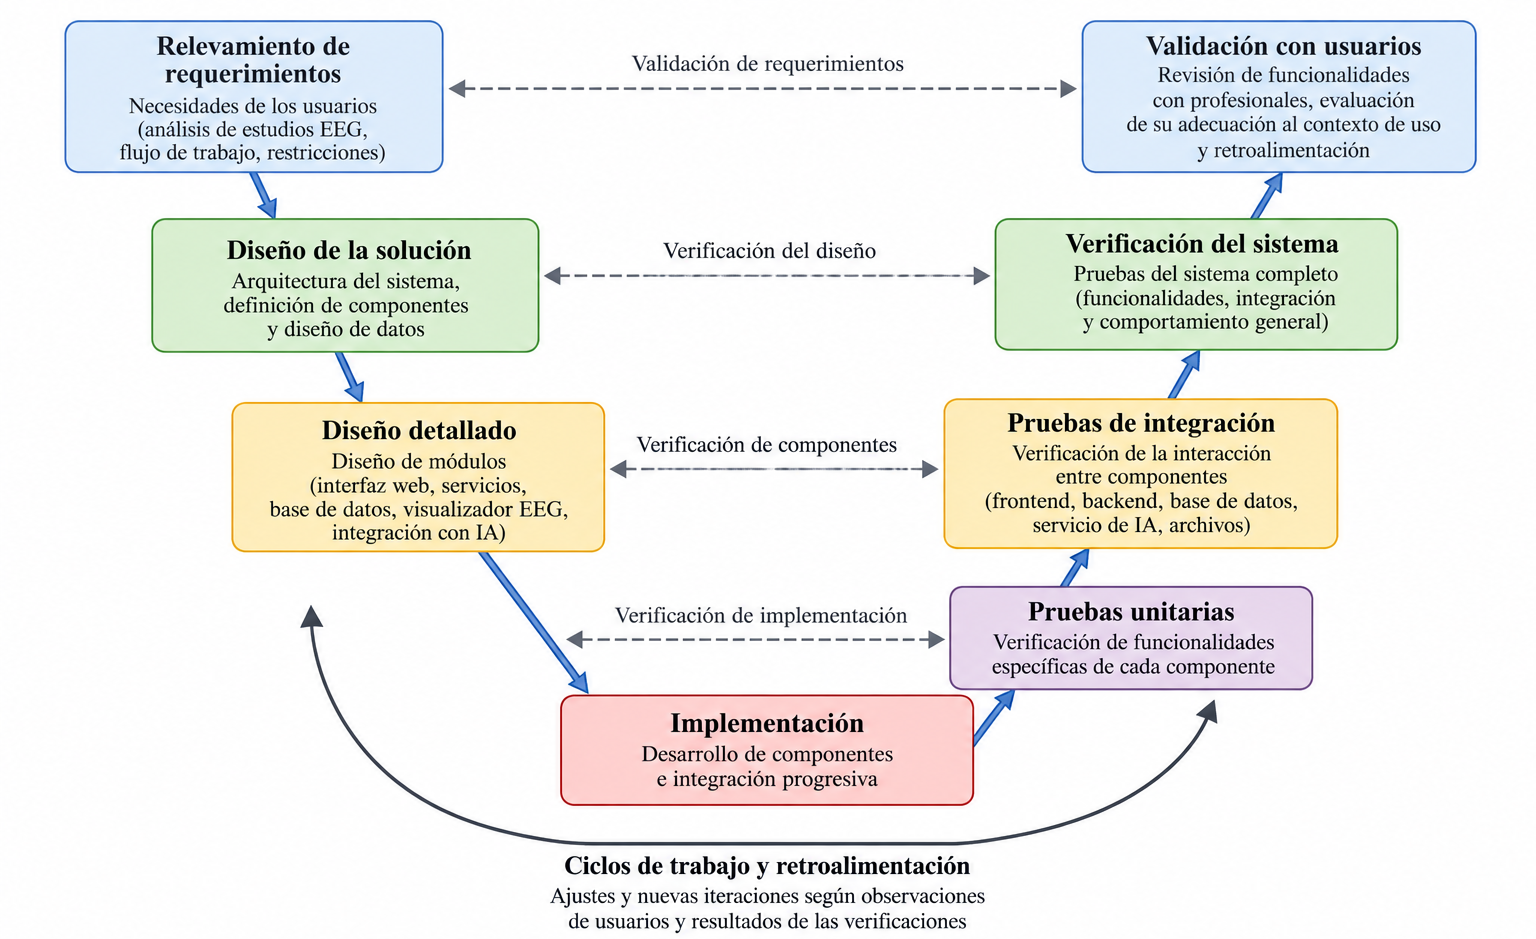
\includegraphics[width=\textwidth]{ThesisFigs/modelo_v_epilexia.png}
    \caption{Adaptación del Modelo V al proceso de desarrollo de EpilexIA.
    Elaboración propia basada en \citet{ForsbergMooz1991}.}
    \label{fig:modelo-v-epilexia}
\end{figure}

Esta adaptación del Modelo V al proceso de desarrollo de EpilexIA se
representa de forma esquemática en la Figura~\ref{fig:modelo-v-epilexia}.
La adaptación permitió conservar la trazabilidad entre las necesidades
identificadas, las decisiones de diseño, las funcionalidades implementadas y
las actividades destinadas a comprobarlas, sin impedir la incorporación de
retroalimentación durante el desarrollo. Las
secciones siguientes describen con mayor detalle las actividades de
relevamiento, diseño, implementación, integración, verificación y validación
realizadas en el proyecto.

\section{Relevamiento de requerimientos}
\label{sec:relevamiento-requerimientos}

El relevamiento de requerimientos constituyó una actividad fundamental para
comprender el contexto de utilización de EpilexIA y definir las funcionalidades
que debía proporcionar el sistema. Este proceso se desarrolló considerando el
flujo de trabajo relacionado con los estudios EEG en el Hospital Central del
Instituto de Previsión Social y las necesidades identificadas durante las
instancias de interacción con los profesionales involucrados.

Durante las primeras etapas del proyecto se analizaron las actividades
relacionadas con la gestión y revisión de estudios electroencefalográficos,
así como las características de las herramientas utilizadas en dicho contexto.
Este análisis permitió identificar necesidades vinculadas con el acceso a los
estudios, la visualización de señales EEG, la gestión de la información
asociada y la elaboración de informes, además de aspectos relacionados con la
seguridad, el control de acceso y la trazabilidad de las operaciones realizadas
en el sistema.

El relevamiento no se limitó a una única etapa inicial. A lo largo del
desarrollo se realizaron reuniones de seguimiento y revisión en las que se
presentaron avances funcionales y se analizaron observaciones sobre el
comportamiento esperado del sistema. Estas instancias permitieron precisar
requerimientos previamente identificados e incorporar ajustes derivados de una
mejor comprensión del flujo de trabajo y de las necesidades de los usuarios.

Los requerimientos relacionados con los perfiles de usuario también
evolucionaron durante el proyecto. Las primeras definiciones contemplaban una
separación más específica de determinados perfiles clínicos. Posteriormente,
a partir de las revisiones realizadas sobre el flujo de trabajo, estas
responsabilidades fueron reorganizadas en perfiles que representaran de forma
más adecuada la utilización prevista del sistema. Como resultado, la
configuración final contempla los perfiles Administrador, Técnico y
Especialista, cada uno asociado con las operaciones que le corresponden dentro
de EpilexIA.

\section{Diseño y desarrollo de la solución}
\label{sec:diseno-desarrollo-solucion}

A partir de los requerimientos identificados se inició el diseño de la solución,
definiendo los principales componentes de EpilexIA y las responsabilidades
asociadas con cada uno de ellos. El sistema fue concebido mediante una
arquitectura modular que permitiera separar la gestión de la información, la
lógica de negocio, la interacción con los usuarios y el procesamiento de las
señales EEG.

El diseño contempló una aplicación web para la interacción con los usuarios,
servicios de \textit{backend} encargados de gestionar la lógica del sistema y el acceso
a los datos, una base de datos para la persistencia de la información y
componentes destinados al procesamiento de los estudios EEG. Asimismo, se
consideró la integración con el servicio de inteligencia artificial encargado
del procesamiento automatizado de las señales, manteniendo separadas las
responsabilidades correspondientes a la aplicación web y al componente de
procesamiento mediante inteligencia artificial.

\section{Desarrollo asistido por inteligencia artificial}
\label{sec:desarrollo-asistido-ia}

La implementación de EpilexIA se realizó con la asistencia de herramientas de inteligencia artificial para la generación y revisión de código.
Los integrantes del equipo utilizaron Claude Code, Cursor y Codex, según la elección de cada desarrollador.

El equipo adoptó para los repositorios del sistema un conjunto de prácticas orientadas a mantener el control sobre el código producido:

\begin{itemize}
    \item \textbf{Contexto explícito por repositorio.}
    Cada repositorio incluye archivos que describen su arquitectura, sus convenciones y las reglas que deben respetar los asistentes (\texttt{CLAUDE.md}, \texttt{AGENTS.md} y reglas de Cursor).
    Estos archivos cumplen la función de documento rector del proyecto y permiten que distintos desarrolladores y herramientas trabajen sobre una base común.

    \item \textbf{Especificación y planificación previas.}
    El sistema cuenta con una especificación general, y los cambios de mayor alcance se elaboraron primero como planes documentados, que se conservan junto al código en la carpeta de documentación de los repositorios.

    \item \textbf{Revisión humana del código.}
    Los cambios se desarrollaron en ramas derivadas de la rama principal y se integraron mediante solicitudes de integración (\textit{pull requests}), revisadas por el líder técnico del equipo antes de su aprobación.

    \item \textbf{Verificación.}
    El código se acompañó de pruebas automatizadas y fue sometido a las actividades de verificación y validación que se describen en las secciones siguientes.
\end{itemize}

Esta forma de trabajo se relaciona con el desarrollo guiado por especificaciones, aunque no se adoptó una metodología formal de ese tipo.
Dentro del Modelo V, las prácticas descritas corresponden a las etapas de implementación y de verificación de componentes.
La asistencia de inteligencia artificial intervino en la producción del código, mientras que la definición de los requerimientos, las decisiones de diseño, la aprobación de los cambios y la validación con la especialista permanecieron a cargo del equipo.

\section{Verificación e integración}
\label{sec:verificacion-integracion}

La verificación de EpilexIA se realizó de manera progresiva durante el
desarrollo, con el propósito de comprobar que las funcionalidades
implementadas respondieran al comportamiento esperado antes de avanzar hacia
su integración con otros componentes. Este proceso permitió detectar
inconsistencias y realizar ajustes durante la construcción del sistema, en
lugar de concentrar las actividades de comprobación únicamente al finalizar
el desarrollo.

La integración con el subsistema de inteligencia artificial contempló
la solicitud de ejecuciones de procesamiento, su identificación y
seguimiento, la consulta de los estados correspondientes y la
recuperación de los resultados asociados con los estudios EEG.
Estas operaciones se verificaron mediante la ejecución del ciclo completo de procesamiento sobre estudios EEG reales, cuyos resultados se documentan en el Capítulo~\ref{pruebas_evaluacion}.

\section{Validación con usuarios}
\label{sec:validacion-usuarios}

Las actividades de validación funcional de EpilexIA comprendieron
instancias de revisión de las funcionalidades implementadas y la
obtención de retroalimentación de usuarios vinculados con el
contexto de utilización del sistema. Estas actividades permitieron
contrastar los avances realizados con las necesidades identificadas
durante el relevamiento y evaluar la adecuación de las
funcionalidades al flujo de trabajo previsto.

En particular, la validación se realizó con una médica especialista en epileptología del Hospital Central del IPS, mediante sesiones semanales desarrolladas en el hospital durante septiembre y octubre de 2026 sobre estudios EEG reales.
Las observaciones formuladas en dichas sesiones y su incorporación al sistema se detallan en el Cuadro~\ref{tab:observaciones-especialista}.

Las revisiones tuvieron especial importancia en las funcionalidades
relacionadas con el trabajo sobre estudios EEG. La disposición de los
elementos del visualizador, la representación de las señales, los controles
destinados al análisis y la organización de la información asociada al estudio
fueron objeto de ajustes durante el desarrollo. De manera similar, se revisaron
aspectos relacionados con los perfiles de usuario, la gestión de estudios, la
elaboración de informes y la presentación de los resultados provenientes del
procesamiento mediante inteligencia artificial.

Estas instancias de validación estuvieron orientadas principalmente a comprobar
la adecuación funcional y de uso de EpilexIA dentro del contexto para el cual
fue desarrollado. Por tanto, deben distinguirse de una validación clínica del
modelo de inteligencia artificial o de una evaluación destinada a establecer
la eficacia diagnóstica del sistema, aspectos que no forman parte del alcance
del presente trabajo.

\section{Ciclos de trabajo y retroalimentación}
\label{sec:ciclos-retroalimentacion}

El desarrollo de EpilexIA se organizó mediante ciclos de trabajo en los que
las actividades de análisis, diseño, implementación, verificación y revisión
se relacionaron de forma continua. Estos ciclos permitieron avanzar sobre
funcionalidades específicas y, al mismo tiempo, incorporar las observaciones
obtenidas durante las reuniones de seguimiento y las revisiones de los avances
del sistema.

En consecuencia, la adaptación metodológica utilizada en EpilexIA conservó la
relación entre requerimientos, diseño, implementación, verificación y
validación planteada por el Modelo V, incorporando ciclos de retroalimentación
cuando las revisiones funcionales o técnicas hacían necesario modificar una
decisión previa. Este enfoque permitió que la solución evolucionara de manera
controlada a partir de las necesidades identificadas y de los resultados
obtenidos durante su desarrollo.



\clearpage
\lhead{\emph{Análisis de requerimientos y diseño}}
\chapter{Análisis de requerimientos y diseño}
\label{cap:analisis-diseno}

\section{Contexto operativo del Hospital Central del IPS}
\label{sec:contexto-operativo-ips}

EpilexIA fue desarrollado considerando el contexto de trabajo relacionado con
los estudios electroencefalográficos en el Hospital Central del Instituto de
Previsión Social (IPS). El análisis de este entorno permitió identificar las
actividades involucradas en la gestión y revisión de los estudios EEG y
establecer las necesidades que posteriormente dieron origen a los
requerimientos del sistema.

En el flujo de trabajo considerado, la adquisición de las señales EEG se
realiza mediante el equipamiento especializado disponible en la institución.
Una vez obtenido el registro, el flujo de trabajo continúa con la revisión
del estudio, el examen de las señales electroencefalográficas y la utilización
de la información obtenida durante el análisis para la elaboración del informe
correspondiente.

El equipamiento utilizado para la adquisición y revisión de los estudios
incluye el sistema Easy III de Cadwell. Este proporciona las funciones
necesarias para registrar y revisar las señales electroencefalográficas; sin
embargo, el proyecto EpilexIA no fue concebido para sustituir el proceso de
adquisición realizado mediante dicho equipamiento. Su alcance se concentra en
las etapas posteriores, una vez que los archivos correspondientes al estudio
se encuentran disponibles para su incorporación al sistema.

Dentro de este contexto se identificó la necesidad de disponer de una
plataforma web que permitiera centralizar diferentes actividades asociadas con
los estudios. Entre ellas se encuentran el registro y la consulta de la información necesaria para identificar a los pacientes y sus estudios, la incorporación de los archivos correspondientes, la visualización de las señales EEG y la elaboración de informes clínicos por parte de los profesionales responsables de su revisión.

A estas necesidades se incorporó la posibilidad de utilizar procesamiento
automatizado mediante inteligencia artificial como apoyo durante el análisis.
Para ello, EpilexIA debía permitir solicitar el procesamiento de un estudio,
recibir los resultados generados y presentarlos junto con la información
necesaria para que el profesional pudiera revisarlos en relación con las
señales EEG. El resultado del procesamiento automatizado no sustituye la
interpretación realizada por el especialista ni constituye por sí mismo un
diagnóstico clínico.

El contexto operativo también hizo necesario considerar diferentes
responsabilidades dentro del sistema. Las actividades relacionadas con la
administración de usuarios, la preparación y gestión de los estudios y la
revisión especializada de las señales requieren distintos niveles de acceso.
Asimismo, las operaciones realizadas sobre la información debían quedar
registradas para facilitar su trazabilidad.

A partir del análisis de este contexto se definieron los actores, requerimientos
y componentes que conforman EpilexIA. Las secciones siguientes presentan estas
definiciones y describen las principales decisiones adoptadas para el diseño de
la solución.

\section{Actores y perfiles de usuario}
\label{sec:actores-perfiles}

A partir del relevamiento de requerimientos y del análisis del flujo de trabajo
se definieron los perfiles de usuario necesarios para representar las
diferentes responsabilidades dentro de EpilexIA. La definición de estos
perfiles permite delimitar las operaciones que puede realizar cada usuario y
constituye la base para el control de acceso aplicado sobre las funcionalidades
del sistema.

Durante el desarrollo, la organización de los perfiles fue objeto de revisión.
Las primeras definiciones contemplaban una separación entre distintos perfiles
clínicos; posteriormente, estas responsabilidades fueron reorganizadas de
acuerdo con las necesidades identificadas durante las revisiones del sistema.
Como resultado, la configuración final de EpilexIA contempla tres perfiles
principales: Administrador, Técnico y Especialista.

El Cuadro~\ref{tab:perfiles-usuario} resume la responsabilidad principal
asociada con cada uno de estos perfiles.

\begin{table}[H]
    \centering
    \caption{Perfiles de usuario definidos en EpilexIA.}
    \label{tab:perfiles-usuario}
    \begin{tabular}{|p{0.20\textwidth}|p{0.68\textwidth}|}
        \hline
        \textbf{Perfil} & \textbf{Responsabilidad principal} \\
        \hline
        Administrador &
        Administración de usuarios y de los aspectos de configuración
        necesarios para la operación del sistema. \\
        \hline
        Técnico &
        Gestión de los datos de los pacientes y estudios,
        incluyendo el registro y la preparación de los estudios EEG para su
        posterior revisión. \\
        \hline
        Especialista &
        Revisión y análisis de los estudios EEG, utilización de las
        herramientas de visualización, revisión de los resultados asociados
        al estudio y elaboración de informes clínicos. \\
        \hline
    \end{tabular}
\end{table}

El perfil \textbf{Administrador} concentra las responsabilidades relacionadas
con la administración del sistema. Entre sus funciones se encuentra la gestión
de los usuarios y de los elementos necesarios para mantener el acceso
controlado a las diferentes funcionalidades. Este perfil se orienta
principalmente a tareas administrativas y de configuración, y no al análisis
clínico de los estudios EEG.

El perfil \textbf{Técnico} participa en las actividades relacionadas con la
preparación y gestión de los estudios. Sus responsabilidades comprenden la
gestión de la información necesaria para identificar al paciente y la creación
y actualización de los estudios EEG. De esta manera, el técnico interviene
principalmente en las etapas previas a la revisión especializada del estudio.

El perfil \textbf{Especialista} representa al profesional responsable de la
revisión de los estudios EEG dentro de EpilexIA. Este perfil dispone de las
funcionalidades necesarias para acceder a los estudios correspondientes,
examinar las señales electroencefalográficas, utilizar las herramientas de
análisis disponibles, revisar la información asociada con eventos y anomalías
y trabajar con los resultados provenientes del procesamiento mediante
inteligencia artificial. Asimismo, puede elaborar y gestionar los informes
clínicos asociados con los estudios y utilizar los mecanismos de colaboración
habilitados por el sistema.

La separación entre estos perfiles responde al principio de asignar las
funcionalidades de acuerdo con las responsabilidades de cada tipo de usuario.
La existencia de un perfil determinado no implica por sí sola el acceso
indiscriminado a todas las operaciones del sistema, ya que las acciones
disponibles se encuentran sujetas a los permisos definidos para cada rol. El
diseño de estos mecanismos de autorización se describe posteriormente en la
sección correspondiente a seguridad y control de acceso.


\section{Requerimientos funcionales}
\label{sec:requerimientos-funcionales}

A partir del análisis del contexto operativo, de los actores identificados y
de las actividades que conforman el flujo de trabajo considerado para
EpilexIA, se definieron los requerimientos funcionales que establecen las
principales capacidades que debe proporcionar el sistema.

Con el propósito de facilitar su organización y mantener una separación
clara entre las distintas responsabilidades funcionales, los requerimientos
se agruparon en siete áreas: administración y acceso, gestión de pacientes,
gestión de estudios EEG, visualización y análisis EEG, procesamiento mediante
inteligencia artificial, informes clínicos y auditoría y trazabilidad.

Cada requerimiento se identifica mediante un código compuesto por el prefijo
RF, seguido de la abreviatura correspondiente al área funcional y un número
correlativo. Esta clasificación permite relacionar posteriormente los
requerimientos con los componentes de diseño, implementación y pruebas
descritos en los capítulos siguientes.

\subsection{Administración y acceso}
\label{subsec:rf-administracion}

Los requerimientos de administración y acceso comprenden las funciones
relacionadas con la autenticación, la administración de cuentas de usuario,
el control de acceso y la recuperación de las credenciales necesarias para
utilizar el sistema. El Cuadro~\ref{tab:rf-adm} presenta los requerimientos
correspondientes a esta área.

\begin{longtable}{|p{0.19\textwidth}|p{0.72\textwidth}|}
    \caption{Requerimientos funcionales de administración y acceso.}
    \label{tab:rf-adm}\\
    \hline
    \textbf{Código} & \textbf{Requerimiento funcional} \\
    \hline
    \endfirsthead

    \hline
    \textbf{Código} & \textbf{Requerimiento funcional} \\
    \hline
    \endhead

    RF-ADM-001 &
    El sistema deberá autenticar a los usuarios registrados antes de permitir
    el acceso a las funcionalidades protegidas. \\
    \hline

    RF-ADM-002 &
    El sistema deberá permitir a los usuarios autorizados listar, buscar y
    filtrar las cuentas de usuario registradas. \\
    \hline

    RF-ADM-003 &
    El sistema deberá permitir a los usuarios autorizados registrar nuevas
    cuentas de usuario. \\
    \hline

    RF-ADM-004 &
    El sistema deberá permitir a los usuarios autorizados modificar la
    información y el rol asignado a una cuenta de usuario. \\
    \hline

    RF-ADM-005 &
    El sistema deberá permitir a los usuarios autorizados activar o desactivar
    cuentas de usuario. \\
    \hline

    RF-ADM-006 &
    El sistema deberá restringir el acceso a sus funcionalidades de acuerdo
    con los permisos asignados al usuario autenticado. \\
    \hline

    RF-ADM-007 &
    El sistema deberá permitir al usuario autenticado cerrar su sesión. \\
    \hline

    RF-ADM-008 &
    El sistema deberá permitir la activación de una cuenta mediante un enlace
    asociado a un \textit{token} de activación válido. \\
    \hline

    RF-ADM-009 &
    El sistema deberá permitir a los usuarios autorizados iniciar o reenviar
    el proceso de recuperación de acceso de una cuenta. \\
    \hline

    RF-ADM-010 &
    El sistema deberá permitir completar el restablecimiento de acceso mediante
    un \textit{token} válido. \\
    \hline

    RF-ADM-011 &
    El sistema deberá permitir al usuario autenticado consultar la información
    de su propio perfil. \\
    \hline

    RF-ADM-012 &
    El sistema deberá permitir a los usuarios autorizados exportar a un archivo
    Excel el listado de usuarios conforme a los criterios de consulta aplicados. \\
    \hline
\end{longtable}

\subsection{Gestión de pacientes}
\label{subsec:rf-pacientes}

Las funcionalidades relacionadas con los pacientes comprenden el registro, la consulta y la actualización de la información necesaria para identificar a las personas asociadas con los estudios EEG. Estas operaciones se integran en el flujo de gestión de estudios, sin constituir un módulo independiente de administración de pacientes. Asimismo, se contempla la consulta de los estudios asociados a cada paciente, de acuerdo con los permisos del usuario. Los requerimientos correspondientes se
presentan en el Cuadro~\ref{tab:rf-pac}.

\begin{longtable}{|p{0.19\textwidth}|p{0.72\textwidth}|}
    \caption{Requerimientos funcionales de gestión de pacientes.}
    \label{tab:rf-pac}\\
    \hline
    \textbf{Código} & \textbf{Requerimiento funcional} \\
    \hline
    \endfirsthead

    \hline
    \textbf{Código} & \textbf{Requerimiento funcional} \\
    \hline
    \endhead

    RF-PAC-001 &
    El sistema deberá permitir a los usuarios autorizados registrar pacientes
    dentro del flujo de gestión de estudios. \\
    \hline

    RF-PAC-002 &
    El sistema deberá permitir a los usuarios autorizados consultar la
    información registrada de un paciente. \\
    \hline

    RF-PAC-003 &
    El sistema deberá permitir a los usuarios autorizados actualizar la
    información registrada de un paciente. \\
    \hline

    RF-PAC-004 &
    El sistema deberá impedir el registro de más de un paciente con el mismo
    documento de identidad. \\
    \hline

    RF-PAC-005 &
    El sistema deberá permitir consultar los estudios asociados a un paciente
    que sean accesibles para el usuario. \\
    \hline
\end{longtable}


\subsection{Gestión de estudios EEG}
\label{subsec:rf-estudios}

Los requerimientos de gestión de estudios EEG comprenden el registro y la
consulta de los estudios, la incorporación de los archivos necesarios para
su análisis y las operaciones relacionadas con su estado y compartición.
El Cuadro~\ref{tab:rf-est} presenta los requerimientos definidos para esta
área.

\begin{longtable}{|p{0.19\textwidth}|p{0.72\textwidth}|}
    \caption{Requerimientos funcionales de gestión de estudios EEG.}
    \label{tab:rf-est}\\
    \hline
    \textbf{Código} & \textbf{Requerimiento funcional} \\
    \hline
    \endfirsthead

    \hline
    \textbf{Código} & \textbf{Requerimiento funcional} \\
    \hline
    \endhead

    RF-EST-001 &
    El sistema deberá permitir a los usuarios autorizados registrar un estudio
    EEG asociado a un paciente y a un Especialista responsable. \\
    \hline

    RF-EST-002 &
    El sistema deberá permitir a los usuarios consultar los estudios EEG a los
    que tengan acceso. \\
    \hline

    RF-EST-003 &
    El sistema deberá permitir buscar y filtrar estudios EEG mediante los
    criterios de consulta disponibles. \\
    \hline

    RF-EST-004 &
    El sistema deberá permitir adjuntar a un estudio los archivos de señales
    EEG en los formatos admitidos. \\
    \hline

    RF-EST-005 &
    El sistema deberá informar el estado de la carga y preparación de los
    archivos asociados al estudio, incluyendo los errores que pudieran
    producirse. \\
    \hline

    RF-EST-006 &
    El sistema deberá permitir asociar un archivo de video al estudio y
    prepararlo para su posterior reproducción cuando sea necesario. \\
    \hline

    RF-EST-007 &
    El sistema deberá permitir consultar el estado y la información general
    de un estudio EEG. \\
    \hline

    RF-EST-008 &
    El sistema deberá permitir a los usuarios autorizados anular un estudio,
    registrando el motivo de la operación. \\
    \hline

    RF-EST-009 &
    El sistema deberá permitir a los usuarios autorizados reactivar un estudio
    previamente anulado, conservando la información relacionada con ambas
    operaciones. \\
    \hline

    RF-EST-010 &
    El sistema deberá permitir a los usuarios autorizados generar, consultar
    y revocar enlaces temporales para compartir un estudio. \\
    \hline

    RF-EST-011 &
    El sistema deberá permitir que un Especialista acceda a un estudio mediante
    un enlace de compartición válido y sea incorporado como observador. \\
    \hline

    RF-EST-012 &
    El sistema deberá permitir consultar los Especialistas observadores
    asociados a un estudio. \\
    \hline
\end{longtable}


\subsection{Visualización y análisis EEG}
\label{subsec:rf-visualizacion}

Esta área reúne las capacidades destinadas a la revisión de las señales EEG
y de la información complementaria asociada al estudio. Incluye las
herramientas de navegación, configuración de la visualización, revisión de
video, eventos e intervalos de interés, así como la presentación de los
resultados provenientes del procesamiento mediante inteligencia artificial.

\begin{longtable}{|p{0.19\textwidth}|p{0.72\textwidth}|}
    \caption{Requerimientos funcionales de visualización y análisis EEG.}
    \label{tab:rf-vis}\\
    \hline
    \textbf{Código} & \textbf{Requerimiento funcional} \\
    \hline
    \endfirsthead

    \hline
    \textbf{Código} & \textbf{Requerimiento funcional} \\
    \hline
    \endhead

    RF-VIS-001 &
    El sistema deberá permitir a los usuarios autorizados acceder al
    visualizador EEG de los estudios disponibles para su revisión. \\
    \hline

    RF-VIS-002 &
    El sistema deberá permitir visualizar las señales EEG correspondientes a
    un intervalo temporal del estudio según el montaje seleccionado. \\
    \hline

    RF-VIS-003 &
    El sistema deberá permitir seleccionar entre los montajes EEG disponibles
    y representar las derivaciones correspondientes. \\
    \hline

    RF-VIS-004 &
    El sistema deberá permitir ajustar los filtros y la sensibilidad utilizados
    para la visualización de las señales EEG. \\
    \hline

    RF-VIS-005 &
    El sistema deberá permitir configurar la visualización de los canales y
    desactivar temporalmente aquellos que no se deseen representar. \\
    \hline

    RF-VIS-006 &
    El sistema deberá permitir desplazarse temporalmente por el registro EEG y
    modificar la ventana de tiempo utilizada para su visualización. \\
    \hline

    RF-VIS-007 &
    El sistema deberá presentar una representación espectrográfica asociada al
    estudio como herramienta complementaria para la revisión de las señales
    EEG. \\
    \hline

    RF-VIS-008 &
    El sistema deberá permitir reproducir el video asociado al estudio de
    manera sincronizada con la posición temporal utilizada durante la revisión
    del EEG. \\
    \hline

    RF-VIS-009 &
    El sistema deberá permitir registrar, consultar y gestionar eventos EEG
    asociados a posiciones o intervalos temporales del estudio. \\
    \hline

    RF-VIS-010 &
    El sistema deberá permitir a los usuarios autorizados identificar
    manualmente intervalos de interés sobre las señales EEG y asociarles
    información descriptiva. \\
    \hline

    RF-VIS-011 &
    El sistema deberá presentar los resultados provenientes del procesamiento
    mediante inteligencia artificial, diferenciándolos de las identificaciones
    manuales y permitiendo su localización temporal sobre las señales EEG. \\
    \hline
\end{longtable}


\subsection{Procesamiento mediante inteligencia artificial}
\label{subsec:rf-ia}

Los requerimientos de esta área describen la interacción de EpilexIA con el
componente de inteligencia artificial integrado al sistema para el
procesamiento de los estudios EEG. Estos requerimientos se refieren a la
solicitud y seguimiento de las ejecuciones, la obtención de resultados y el
registro de información derivada de su revisión por parte del Especialista.
El desarrollo y entrenamiento del modelo de inteligencia artificial no forman
parte del alcance de este trabajo.

\begin{longtable}{|p{0.19\textwidth}|p{0.72\textwidth}|}
    \caption{Requerimientos funcionales de procesamiento mediante inteligencia artificial.}
    \label{tab:rf-ia}\\
    \hline
    \textbf{Código} & \textbf{Requerimiento funcional} \\
    \hline
    \endfirsthead

    \hline
    \textbf{Código} & \textbf{Requerimiento funcional} \\
    \hline
    \endhead

    RF-IA-001 &
    El sistema deberá permitir solicitar el procesamiento mediante inteligencia
    artificial de un estudio EEG autorizado. \\
    \hline

    RF-IA-002 &
    El sistema deberá permitir consultar el estado de una ejecución de
    procesamiento mediante inteligencia artificial. \\
    \hline

    RF-IA-003 &
    El sistema deberá impedir la existencia simultánea de ejecuciones
    equivalentes de procesamiento para un mismo estudio. \\
    \hline

    RF-IA-004 &
    El sistema deberá permitir cancelar una ejecución de procesamiento
    pendiente o en curso cuando su estado lo permita. \\
    \hline

    RF-IA-005 &
    El sistema deberá permitir procesar las señales EEG mediante el componente
    de inteligencia artificial integrado y registrar los resultados obtenidos. \\
    \hline

    RF-IA-006 &
    El sistema deberá permitir consultar los resultados obtenidos mediante
    inteligencia artificial y su ubicación temporal dentro del estudio EEG. \\
    \hline

    RF-IA-007 &
    El sistema deberá permitir registrar y sincronizar las anotaciones manuales
    aportadas por el Especialista como retroalimentación asociada al
    procesamiento. \\
    \hline

    RF-IA-008 &
    El sistema deberá permitir registrar y sincronizar la validación o
    clasificación clínica realizada por el Especialista sobre los resultados
    obtenidos mediante inteligencia artificial. \\
    \hline
\end{longtable}


\subsection{Informes clínicos}
\label{subsec:rf-informes}

Los requerimientos relacionados con los informes clínicos comprenden la
creación, consulta, edición y cierre de los informes elaborados por los
Especialistas, así como la incorporación de información obtenida durante la
revisión de las señales EEG.

\begin{longtable}{|p{0.19\textwidth}|p{0.72\textwidth}|}
    \caption{Requerimientos funcionales de informes clínicos.}
    \label{tab:rf-inf}\\
    \hline
    \textbf{Código} & \textbf{Requerimiento funcional} \\
    \hline
    \endfirsthead

    \hline
    \textbf{Código} & \textbf{Requerimiento funcional} \\
    \hline
    \endhead

    RF-INF-001 &
    El sistema deberá permitir consultar los informes clínicos asociados a un
    estudio EEG. \\
    \hline

    RF-INF-002 &
    El sistema deberá permitir identificar al Especialista responsable de cada
    informe y consultar los informes de otros profesionales cuando el usuario
    tenga acceso al estudio. \\
    \hline

    RF-INF-003 &
    El sistema deberá permitir que un Especialista autorizado cree su propio
    informe clínico para un estudio EEG. \\
    \hline

    RF-INF-004 &
    El sistema deberá permitir al propietario de un informe actualizar su
    contenido mientras este permanezca editable. \\
    \hline

    RF-INF-005 &
    El sistema deberá impedir la modificación de informes pertenecientes a
    otros Especialistas y restringir la edición ordinaria de los informes
    cerrados. \\
    \hline

    RF-INF-006 &
    El sistema deberá permitir incorporar al informe segmentos identificados
    manualmente durante la revisión de las señales EEG. \\
    \hline

    RF-INF-007 &
    El sistema deberá permitir incorporar al informe resultados provenientes
    del procesamiento mediante inteligencia artificial y registrar su
    clasificación clínica. \\
    \hline

    RF-INF-008 &
    El sistema deberá permitir utilizar los segmentos asociados al informe para
    localizar los intervalos correspondientes dentro del registro EEG. \\
    \hline

    RF-INF-009 &
    El sistema deberá permitir al propietario cerrar su informe clínico y
    restringir posteriores modificaciones mediante el flujo ordinario. \\
    \hline

    RF-INF-010 &
    El sistema deberá permitir generar el informe clínico en formato PDF. \\
    \hline
\end{longtable}


\subsection{Auditoría y trazabilidad}
\label{subsec:rf-auditoria}

Los requerimientos de auditoría y trazabilidad establecen las capacidades
destinadas al registro y consulta de las operaciones relevantes realizadas
en el sistema. Su propósito es conservar información que permita identificar
las acciones registradas y el contexto en el que fueron efectuadas.

\begin{longtable}{|p{0.19\textwidth}|p{0.72\textwidth}|}
    \caption{Requerimientos funcionales de auditoría y trazabilidad.}
    \label{tab:rf-aud}\\
    \hline
    \textbf{Código} & \textbf{Requerimiento funcional} \\
    \hline
    \endfirsthead

    \hline
    \textbf{Código} & \textbf{Requerimiento funcional} \\
    \hline
    \endhead

    RF-AUD-001 &
    El sistema deberá permitir a los usuarios autorizados consultar el
    historial paginado de eventos de auditoría registrados. \\
    \hline

    RF-AUD-002 &
    El sistema deberá presentar para cada evento de auditoría la fecha y hora,
    la acción realizada, el actor, el rol y el contexto asociado. \\
    \hline

    RF-AUD-003 &
    El sistema deberá permitir filtrar los eventos de auditoría por fecha,
    acción, actor y rol, pudiendo combinar los criterios disponibles. \\
    \hline

    RF-AUD-004 &
    El sistema deberá permitir ordenar cronológicamente los eventos de
    auditoría. \\
    \hline

    RF-AUD-005 &
    El sistema deberá presentar en el \textit{Dashboard} la actividad reciente
    registrada en la auditoría. \\
    \hline

    RF-AUD-006 &
    El sistema deberá registrar la trazabilidad de las operaciones de negocio
    catalogadas para auditoría, conservando la identificación descriptiva y el
    rol del actor correspondientes al momento de la operación. \\
    \hline
\end{longtable}


\section{Requerimientos no funcionales}
\label{sec:requerimientos-no-funcionales}

Además de las capacidades funcionales descritas en la sección anterior, se
definieron requerimientos no funcionales relacionados con las características
de calidad y las restricciones generales que debe satisfacer EpilexIA. Estos
requerimientos consideran aspectos de rendimiento, seguridad, usabilidad y
compatibilidad, confiabilidad e integridad, mantenibilidad e interoperabilidad,
así como portabilidad y despliegue.

Los requerimientos fueron establecidos considerando las características del
entorno de utilización del sistema y las necesidades derivadas del manejo de
estudios EEG e información asociada. Los requerimientos no funcionales se presentan
agrupados según la característica de calidad a la que se encuentran asociados.

\subsection{Rendimiento}
\label{subsec:rnf-rendimiento}

Los requerimientos de rendimiento consideran especialmente el volumen de
información generado por los estudios EEG y la necesidad de permitir su
exploración mediante la interfaz del sistema.

\begin{longtable}{|p{0.19\textwidth}|p{0.72\textwidth}|}
    \caption{Requerimientos no funcionales de rendimiento.}
    \label{tab:rnf-rendimiento}\\
    \hline
    \textbf{Código} & \textbf{Requerimiento no funcional} \\
    \hline
    \endfirsthead

    \hline
    \textbf{Código} & \textbf{Requerimiento no funcional} \\
    \hline
    \endhead

    RNF-REN-001 &
    El sistema deberá permitir la visualización y navegación de registros EEG
    de gran volumen mediante mecanismos que limiten la cantidad de información
    procesada simultáneamente por la interfaz. \\
    \hline
\end{longtable}


\subsection{Seguridad}
\label{subsec:rnf-seguridad}

Los requerimientos de seguridad establecen las condiciones generales para
proteger el acceso al sistema, las credenciales de los usuarios y las
comunicaciones realizadas en el entorno de despliegue.

\begin{longtable}{|p{0.19\textwidth}|p{0.72\textwidth}|}
    \caption{Requerimientos no funcionales de seguridad.}
    \label{tab:rnf-seguridad}\\
    \hline
    \textbf{Código} & \textbf{Requerimiento no funcional} \\
    \hline
    \endfirsthead

    \hline
    \textbf{Código} & \textbf{Requerimiento no funcional} \\
    \hline
    \endhead

    RNF-SEG-001 &
    El sistema deberá proteger el acceso a las funcionalidades y recursos
    mediante mecanismos de autenticación y autorización basados en los
    permisos del usuario. \\
    \hline

    RNF-SEG-002 &
    Las contraseñas de los usuarios deberán almacenarse mediante mecanismos
    criptográficos de hash, evitando su almacenamiento en texto plano. \\
    \hline

    RNF-SEG-003 &
    El entorno de despliegue del sistema deberá proteger las comunicaciones
    mediante HTTPS. \\
    \hline
\end{longtable}


\subsection{Usabilidad y compatibilidad}
\label{subsec:rnf-usabilidad}

Los requerimientos de usabilidad y compatibilidad buscan favorecer el acceso
a las funcionalidades del sistema desde los dispositivos y navegadores
previstos para su utilización, manteniendo una presentación comprensible para
los diferentes perfiles de usuario.

\begin{longtable}{|p{0.19\textwidth}|p{0.72\textwidth}|}
    \caption{Requerimientos no funcionales de usabilidad y compatibilidad.}
    \label{tab:rnf-usabilidad}\\
    \hline
    \textbf{Código} & \textbf{Requerimiento no funcional} \\
    \hline
    \endfirsthead

    \hline
    \textbf{Código} & \textbf{Requerimiento no funcional} \\
    \hline
    \endhead

    RNF-USA-001 &
    La interfaz deberá presentar las funcionalidades y la información de
    manera clara y comprensible para los perfiles de usuario definidos. \\
    \hline

    RNF-USA-002 &
    La interfaz deberá adaptarse a diferentes tamaños de pantalla, incluyendo
    computadoras y tablets. \\
    \hline

    RNF-USA-003 &
    El sistema deberá ser accesible mediante navegadores web modernos
    compatibles con las tecnologías utilizadas por la aplicación. \\
    \hline

    RNF-USA-004 &
    La interfaz de usuario deberá utilizar el español como idioma principal. \\
    \hline
\end{longtable}


\subsection{Confiabilidad e integridad}
\label{subsec:rnf-confiabilidad}

Estos requerimientos establecen las condiciones relacionadas con la
consistencia de la información, la conservación de las relaciones entre las
entidades administradas por el sistema y el tratamiento de operaciones que no
puedan completarse correctamente.

\begin{longtable}{|p{0.19\textwidth}|p{0.72\textwidth}|}
    \caption{Requerimientos no funcionales de confiabilidad e integridad.}
    \label{tab:rnf-confiabilidad}\\
    \hline
    \textbf{Código} & \textbf{Requerimiento no funcional} \\
    \hline
    \endfirsthead

    \hline
    \textbf{Código} & \textbf{Requerimiento no funcional} \\
    \hline
    \endhead

    RNF-CON-001 &
    El sistema deberá preservar la consistencia de la información ante errores
    producidos durante las operaciones de registro y procesamiento. \\
    \hline

    RNF-CON-002 &
    El sistema deberá mantener la integridad de las relaciones entre pacientes,
    estudios, informes y demás información asociada. \\
    \hline

    RNF-CON-003 &
    El sistema deberá informar los errores producidos durante operaciones que
    no puedan completarse correctamente, evitando presentar como exitosas
    operaciones incompletas. \\
    \hline
\end{longtable}


\subsection{Mantenibilidad e interoperabilidad}
\label{subsec:rnf-mantenibilidad}

Los requerimientos de mantenibilidad e interoperabilidad consideran la
organización de los componentes del sistema y la definición de mecanismos de
comunicación que faciliten su mantenimiento, evolución e integración.

\begin{longtable}{|p{0.19\textwidth}|p{0.72\textwidth}|}
    \caption{Requerimientos no funcionales de mantenibilidad e interoperabilidad.}
    \label{tab:rnf-mantenibilidad}\\
    \hline
    \textbf{Código} & \textbf{Requerimiento no funcional} \\
    \hline
    \endfirsthead

    \hline
    \textbf{Código} & \textbf{Requerimiento no funcional} \\
    \hline
    \endhead

    RNF-MAN-001 &
    El sistema deberá mantener una separación modular de responsabilidades que
    facilite su mantenimiento y evolución. \\
    \hline

    RNF-MAN-002 &
    Los servicios de comunicación entre los componentes del sistema deberán
    utilizar interfaces claramente definidas. \\
    \hline

    RNF-MAN-003 &
    La interfaz de servicios del \textit{backend} deberá disponer de documentación que
    facilite su consulta, prueba e integración. \\
    \hline
\end{longtable}


\subsection{Portabilidad y despliegue}
\label{subsec:rnf-portabilidad}

Los requerimientos de portabilidad y despliegue establecen las condiciones
generales relacionadas con las tecnologías utilizadas y la posibilidad de
desplegar los componentes de EpilexIA en entornos reproducibles.

\begin{longtable}{|p{0.19\textwidth}|p{0.72\textwidth}|}
    \caption{Requerimientos no funcionales de portabilidad y despliegue.}
    \label{tab:rnf-portabilidad}\\
    \hline
    \textbf{Código} & \textbf{Requerimiento no funcional} \\
    \hline
    \endfirsthead

    \hline
    \textbf{Código} & \textbf{Requerimiento no funcional} \\
    \hline
    \endhead

    RNF-POR-001 &
    Los componentes desarrollados para EpilexIA deberán utilizar tecnologías
    y herramientas de código abierto compatibles con los requerimientos del
    proyecto. \\
    \hline

    RNF-POR-002 &
    El sistema deberá permitir el despliegue de sus componentes en entornos
    contenedorizados. \\
    \hline
\end{longtable}


\section{Diagramas de secuencia}
\label{sec:diagramas-secuencia}

Los diagramas de secuencia permiten representar las interacciones
entre los actores y los componentes del sistema durante la ejecución
de determinados procesos. Su utilización facilita la comprensión
del intercambio de solicitudes, respuestas e información entre
los elementos que conforman EpilexIA.

Para describir el comportamiento de la solución se seleccionaron cinco procesos representativos, considerando su importancia dentro del flujo de trabajo y su relación con los requerimientos funcionales definidos anteriormente.

Los diagramas presentan las principales interacciones entre
los usuarios, la interfaz web, los servicios del \textit{backend},
la base de datos y, cuando corresponde, el componente de
inteligencia artificial integrado al sistema.

\subsection{Autenticación de usuario}
\label{subsec:secuencia-autenticacion}

El proceso de autenticación permite verificar la identidad
de los usuarios antes de concederles acceso a las
funcionalidades protegidas de EpilexIA.

La solicitud se origina en la interfaz web y es procesada
por el \textit{backend}, que consulta la información del usuario
y verifica las credenciales proporcionadas. Cuando la autenticación es satisfactoria, se registra la sesión correspondiente y se devuelve el \textit{token} necesario para las solicitudes posteriores. En caso contrario, se
informa el error sin habilitar el acceso.

La Figura~\ref{fig:secuencia-autenticacion} presenta
las interacciones principales de este proceso.

\begin{figure}[H]
    \centering
    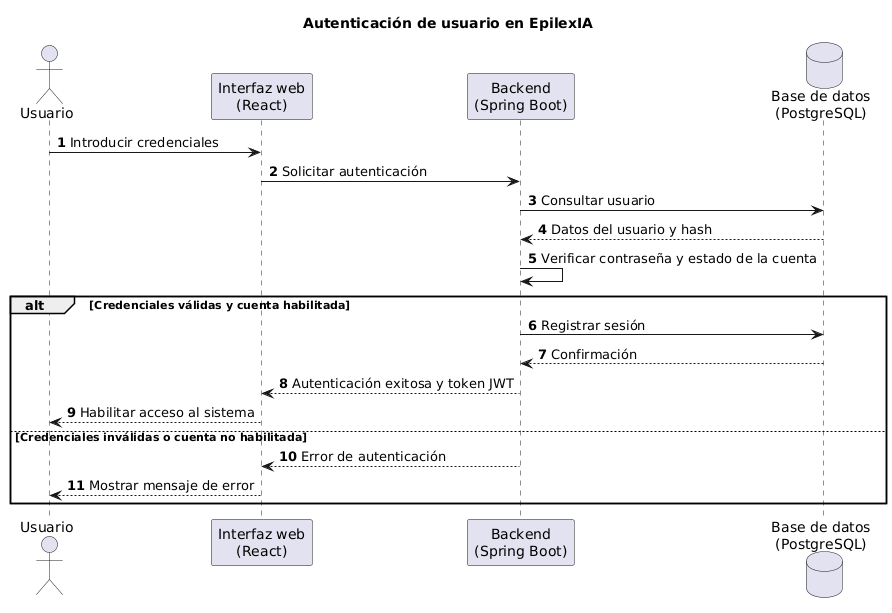
\includegraphics[width=0.95\textwidth]
    {ThesisFigs/secuencia_autenticacion.png}
    \caption{Diagrama de secuencia del proceso de
    autenticación de usuario en EpilexIA.
    Elaboración propia.}
    \label{fig:secuencia-autenticacion}
\end{figure}


\subsection{Registro y preparación de un estudio EEG}
\label{subsec:secuencia-registro-estudio}

El proceso de registro y preparación de un estudio EEG
comprende la identificación del paciente, la creación
del estudio y la incorporación de los archivos asociados.
Estas actividades se desarrollan en etapas diferenciadas,
que permiten gestionar el registro y el procesamiento
de las señales electroencefalográficas.

En la primera etapa, el usuario autorizado selecciona
un paciente existente o incorpora uno nuevo. Posteriormente,
completa la información del estudio, selecciona el archivo
EEG en formato EDF y, cuando corresponde, identifica
al Especialista responsable de su revisión. El \textit{backend}
verifica los datos y registra el estudio con estado inicial
Pendiente.

La Figura~\ref{fig:secuencia-registro-estudio} presenta
las principales interacciones de esta primera etapa.

\begin{figure}[H]
    \centering
    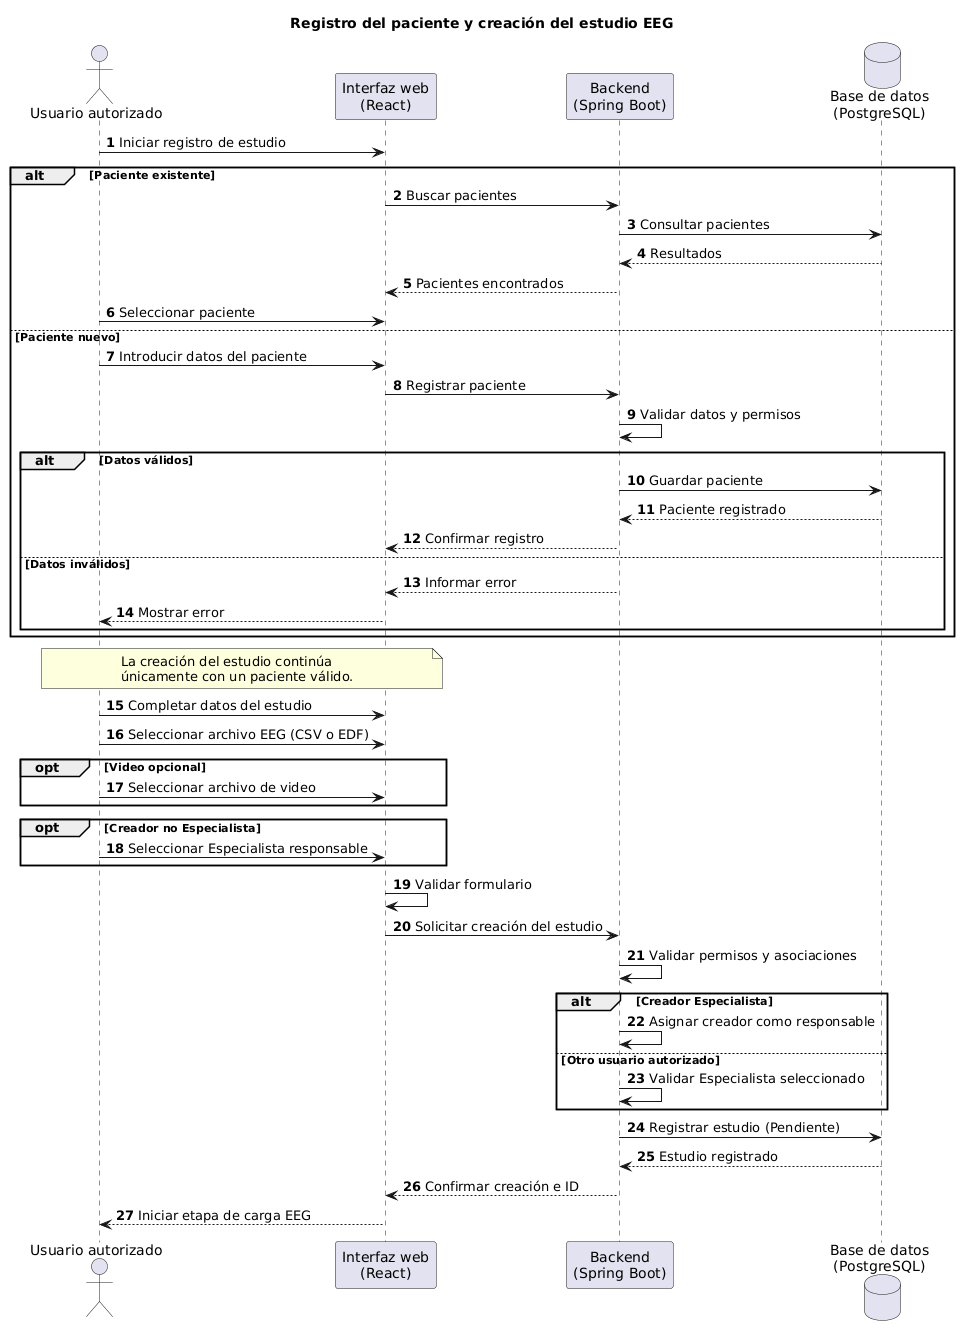
\includegraphics[
        width=\textwidth,
        height=0.82\textheight,
        keepaspectratio
    ]{ThesisFigs/secuencia_registro_estudio.png}
    \caption{Diagrama de secuencia del registro del paciente
    y creación del estudio EEG en EpilexIA.
    Elaboración propia.}
    \label{fig:secuencia-registro-estudio}
\end{figure}

Una vez registrado el estudio, el archivo EEG se transmite
al \textit{backend} mediante fragmentos. Al finalizar la carga,
se inicia el procesamiento correspondiente de manera
asíncrona. Durante esta etapa, la interfaz consulta
periódicamente el estado del estudio hasta obtener
un resultado de procesamiento exitoso o un error.

La Figura~\ref{fig:secuencia-preparacion-eeg} representa
la carga y preparación del archivo EEG, así como
el seguimiento de su estado.

\begin{figure}[H]
    \centering
    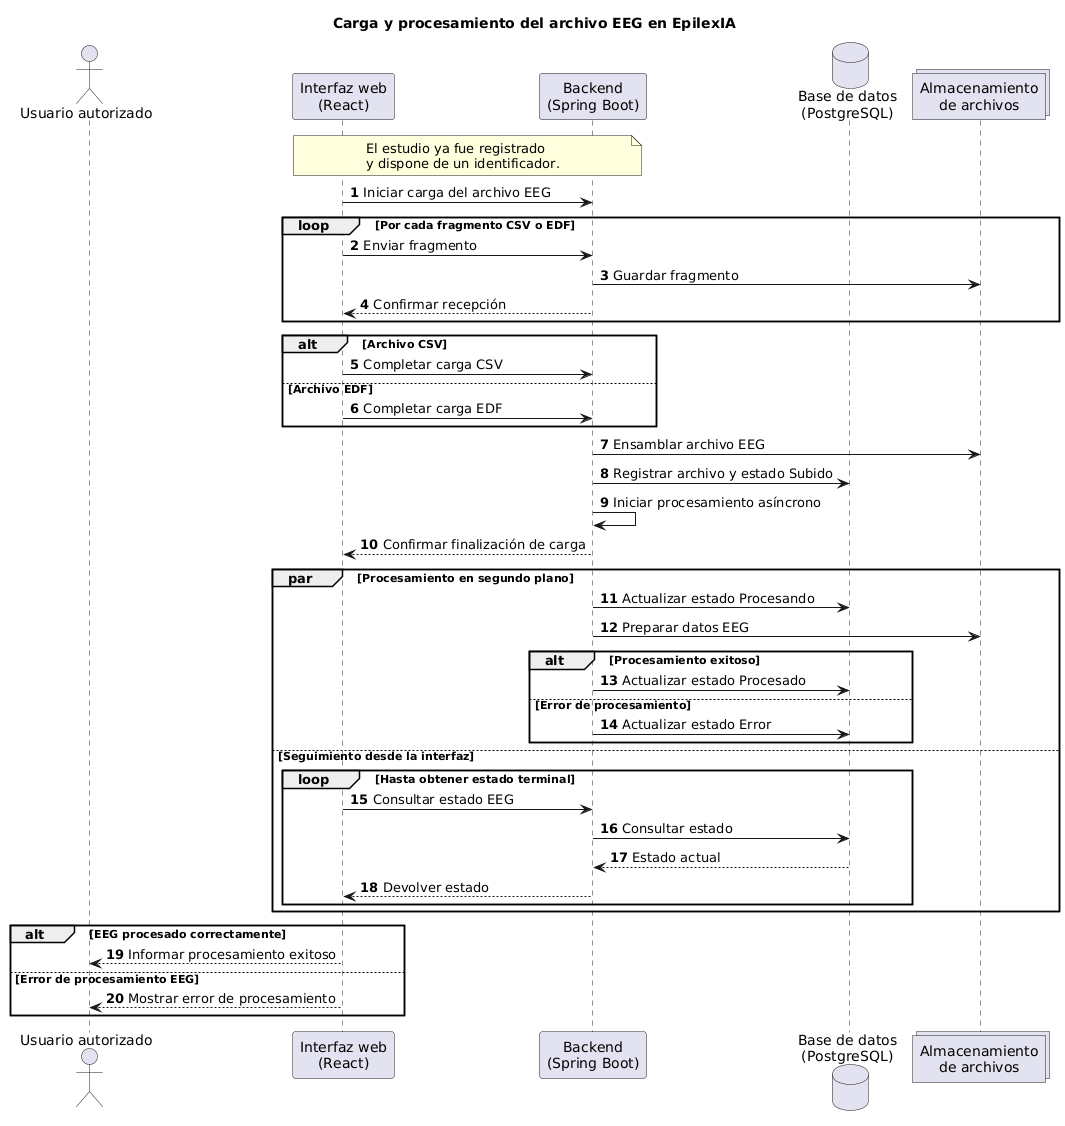
\includegraphics[
        width=\textwidth,
        height=0.82\textheight,
        keepaspectratio
    ]{ThesisFigs/secuencia_carga_procesamiento_eeg.png}
    \caption{Diagrama de secuencia de la carga y
    procesamiento del archivo EEG en EpilexIA.
    Elaboración propia.}
    \label{fig:secuencia-preparacion-eeg}
\end{figure}

Cuando el procesamiento del EEG finaliza correctamente,
el sistema permite continuar con la incorporación
de un video asociado, si corresponde. Los archivos
MP4 se gestionan mediante un procedimiento de carga
y almacenamiento, mientras que los archivos EZVideo
requieren un proceso adicional de conversión a MP4.

La Figura~\ref{fig:secuencia-carga-video} muestra
las interacciones correspondientes a la carga y
preparación del video, incluyendo el seguimiento
de la conversión cuando se utiliza el formato EZVideo.

\begin{figure}[H]
    \centering
    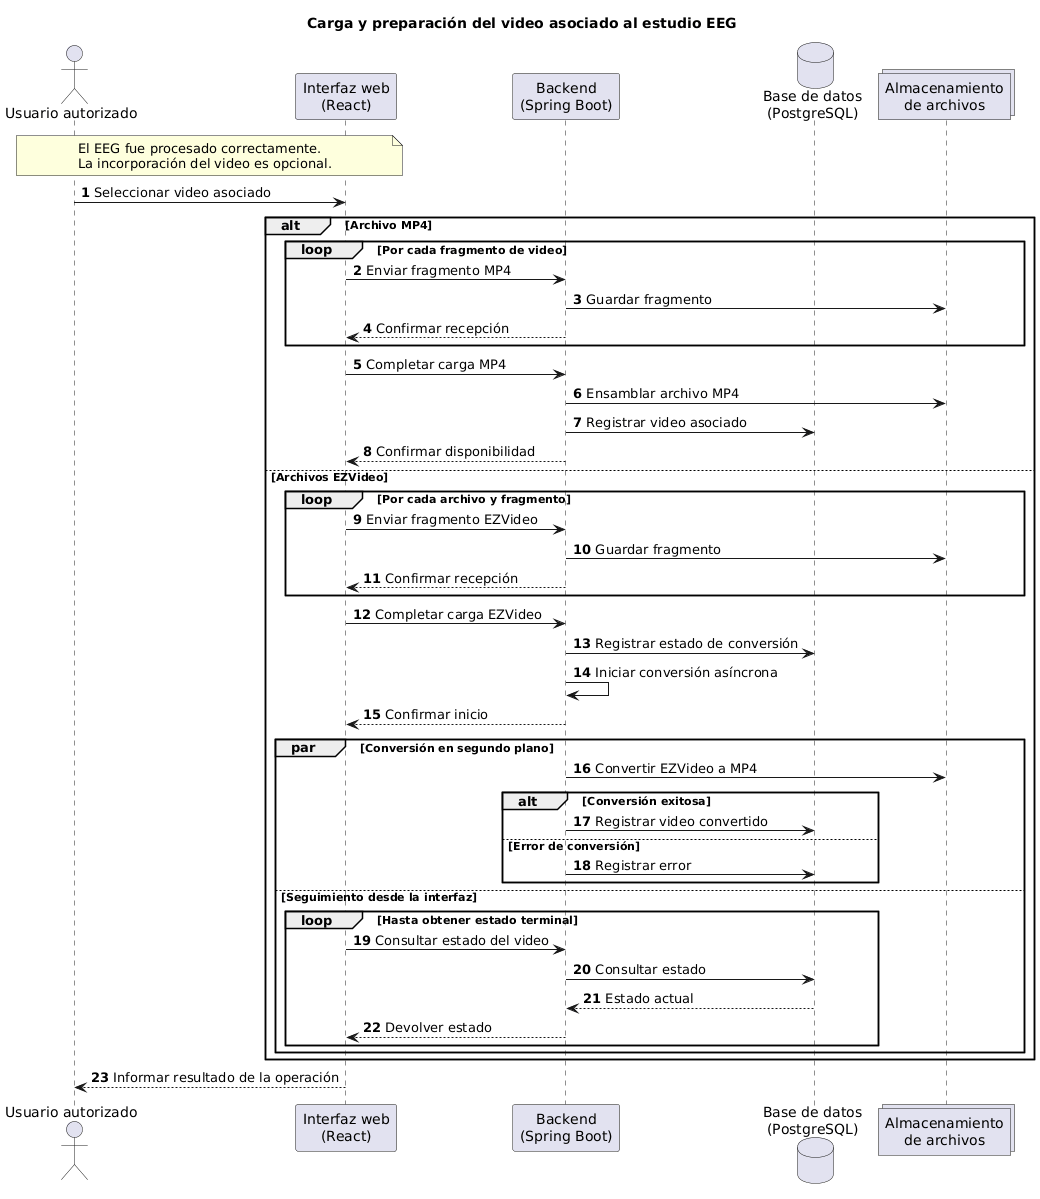
\includegraphics[
        width=\textwidth,
        height=0.82\textheight,
        keepaspectratio
    ]{ThesisFigs/secuencia_carga_video.png}
    \caption{Diagrama de secuencia de la carga y
    preparación del video asociado a un estudio EEG.
    Elaboración propia.}
    \label{fig:secuencia-carga-video}
\end{figure}


\subsection{Visualización de señales EEG}
\label{subsec:secuencia-visualizacion-eeg}

La visualización de señales EEG constituye una de las
funcionalidades principales de EpilexIA, ya que permite
al Especialista examinar los registros
electroencefalográficos asociados a un estudio.

El proceso comienza cuando el usuario autorizado accede
al visualizador. El sistema consulta la información del
estudio, verifica las condiciones de acceso y obtiene
los metadatos necesarios para presentar las señales.
Asimismo, recupera los montajes disponibles y establece
la configuración inicial de visualización.

Las señales EEG se obtienen mediante solicitudes de
segmentos correspondientes a intervalos temporales.
El \textit{backend} recupera los datos almacenados, aplica
los filtros configurados y organiza las derivaciones
según el montaje seleccionado. Posteriormente, la
interfaz web presenta las señales mediante una
representación gráfica multicanal.

La Figura~\ref{fig:secuencia-inicializacion-visualizador-eeg}
representa las principales interacciones correspondientes
al acceso al estudio, la recuperación de información y
la carga inicial de las señales EEG.

\begin{figure}[H]
    \centering
    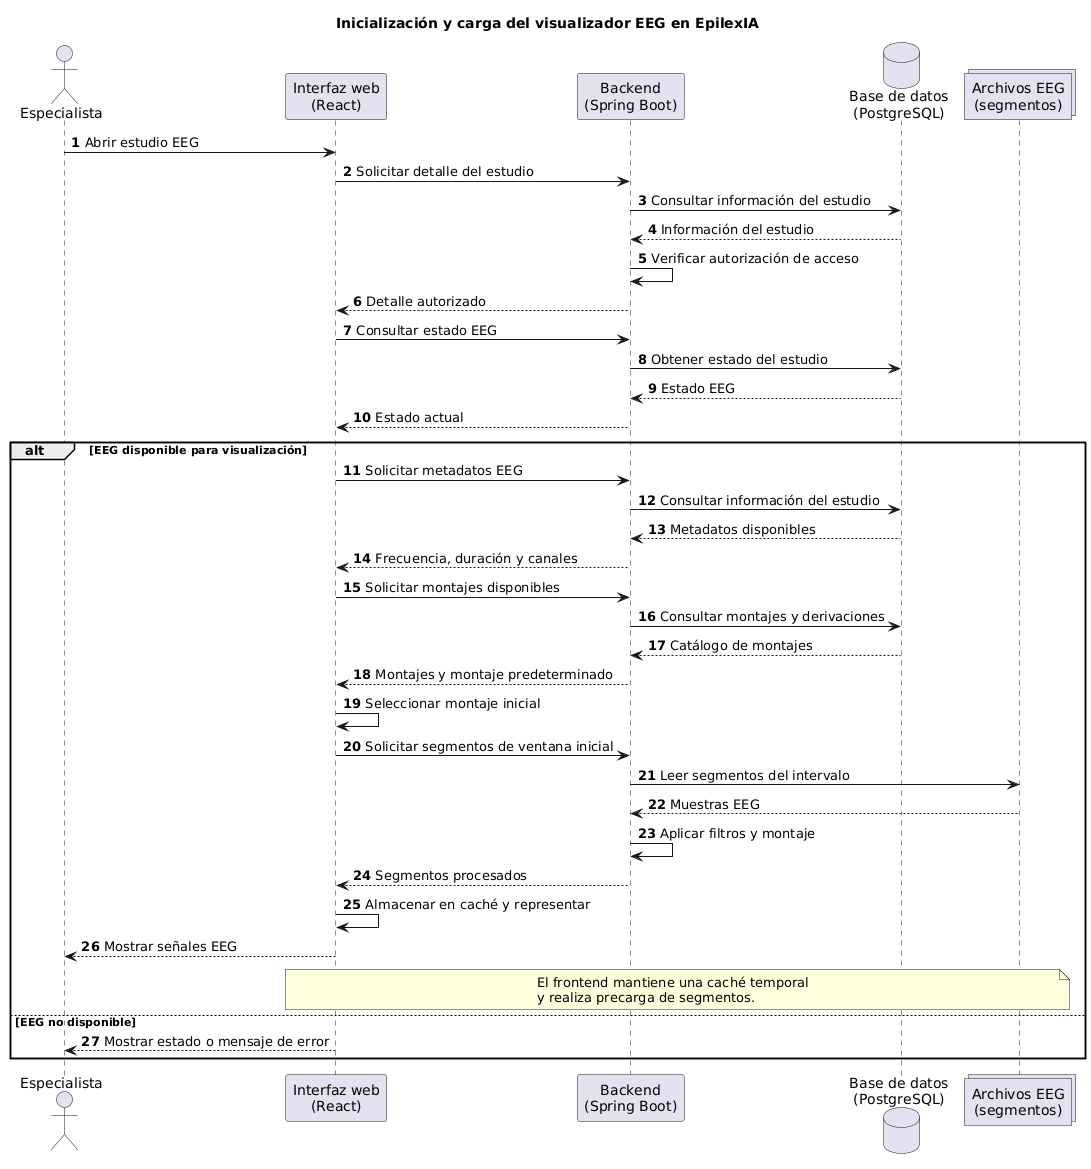
\includegraphics[
        width=\textwidth,
        height=0.82\textheight,
        keepaspectratio
    ]{ThesisFigs/secuencia_inicializacion_visualizador_eeg.png}
    \caption{Diagrama de secuencia de la inicialización
    y carga del visualizador EEG en EpilexIA.
    Elaboración propia.}
    \label{fig:secuencia-inicializacion-visualizador-eeg}
\end{figure}


Durante la revisión del estudio, el Especialista puede
desplazarse entre diferentes intervalos temporales,
seleccionar montajes y ajustar los filtros y la
sensibilidad de las señales. La navegación temporal
contempla dos modalidades complementarias: el
desplazamiento por segundos mediante los controles
de avance y retroceso, y el desplazamiento por ventanas
completas mediante las flechas horizontales del teclado.
La duración de cada ventana puede configurarse entre
5 y 25 segundos.

Asimismo, el Especialista puede modificar la
sensibilidad mediante las flechas verticales del
teclado, lo que permite ajustar la escala de
representación sin interrumpir la revisión del estudio.
Cuando existe un video asociado, la navegación
temporal mantiene la sincronización entre el cursor
EEG y la posición del video.

Para facilitar estas operaciones, el visualizador
mantiene temporalmente en memoria los segmentos
consultados y realiza una precarga de datos. Cuando
la información necesaria se encuentra disponible
en la caché, la representación gráfica puede
actualizarse sin realizar nuevas solicitudes al servidor.

El cambio de montaje o de filtros puede requerir
la recuperación y el procesamiento de nuevos segmentos
por parte del \textit{backend}. En cambio, el ajuste de
sensibilidad modifica la escala vertical de las señales
desde la interfaz web, sin necesidad de recuperar
nuevamente las muestras EEG. La sensibilidad
seleccionada puede conservarse como preferencia
del usuario.

La Figura~\ref{fig:secuencia-interacciones-visualizador-eeg}
presenta las interacciones correspondientes a la
navegación temporal, el cambio de montaje y los
ajustes de filtros y sensibilidad.

\begin{figure}[H]
    \centering
    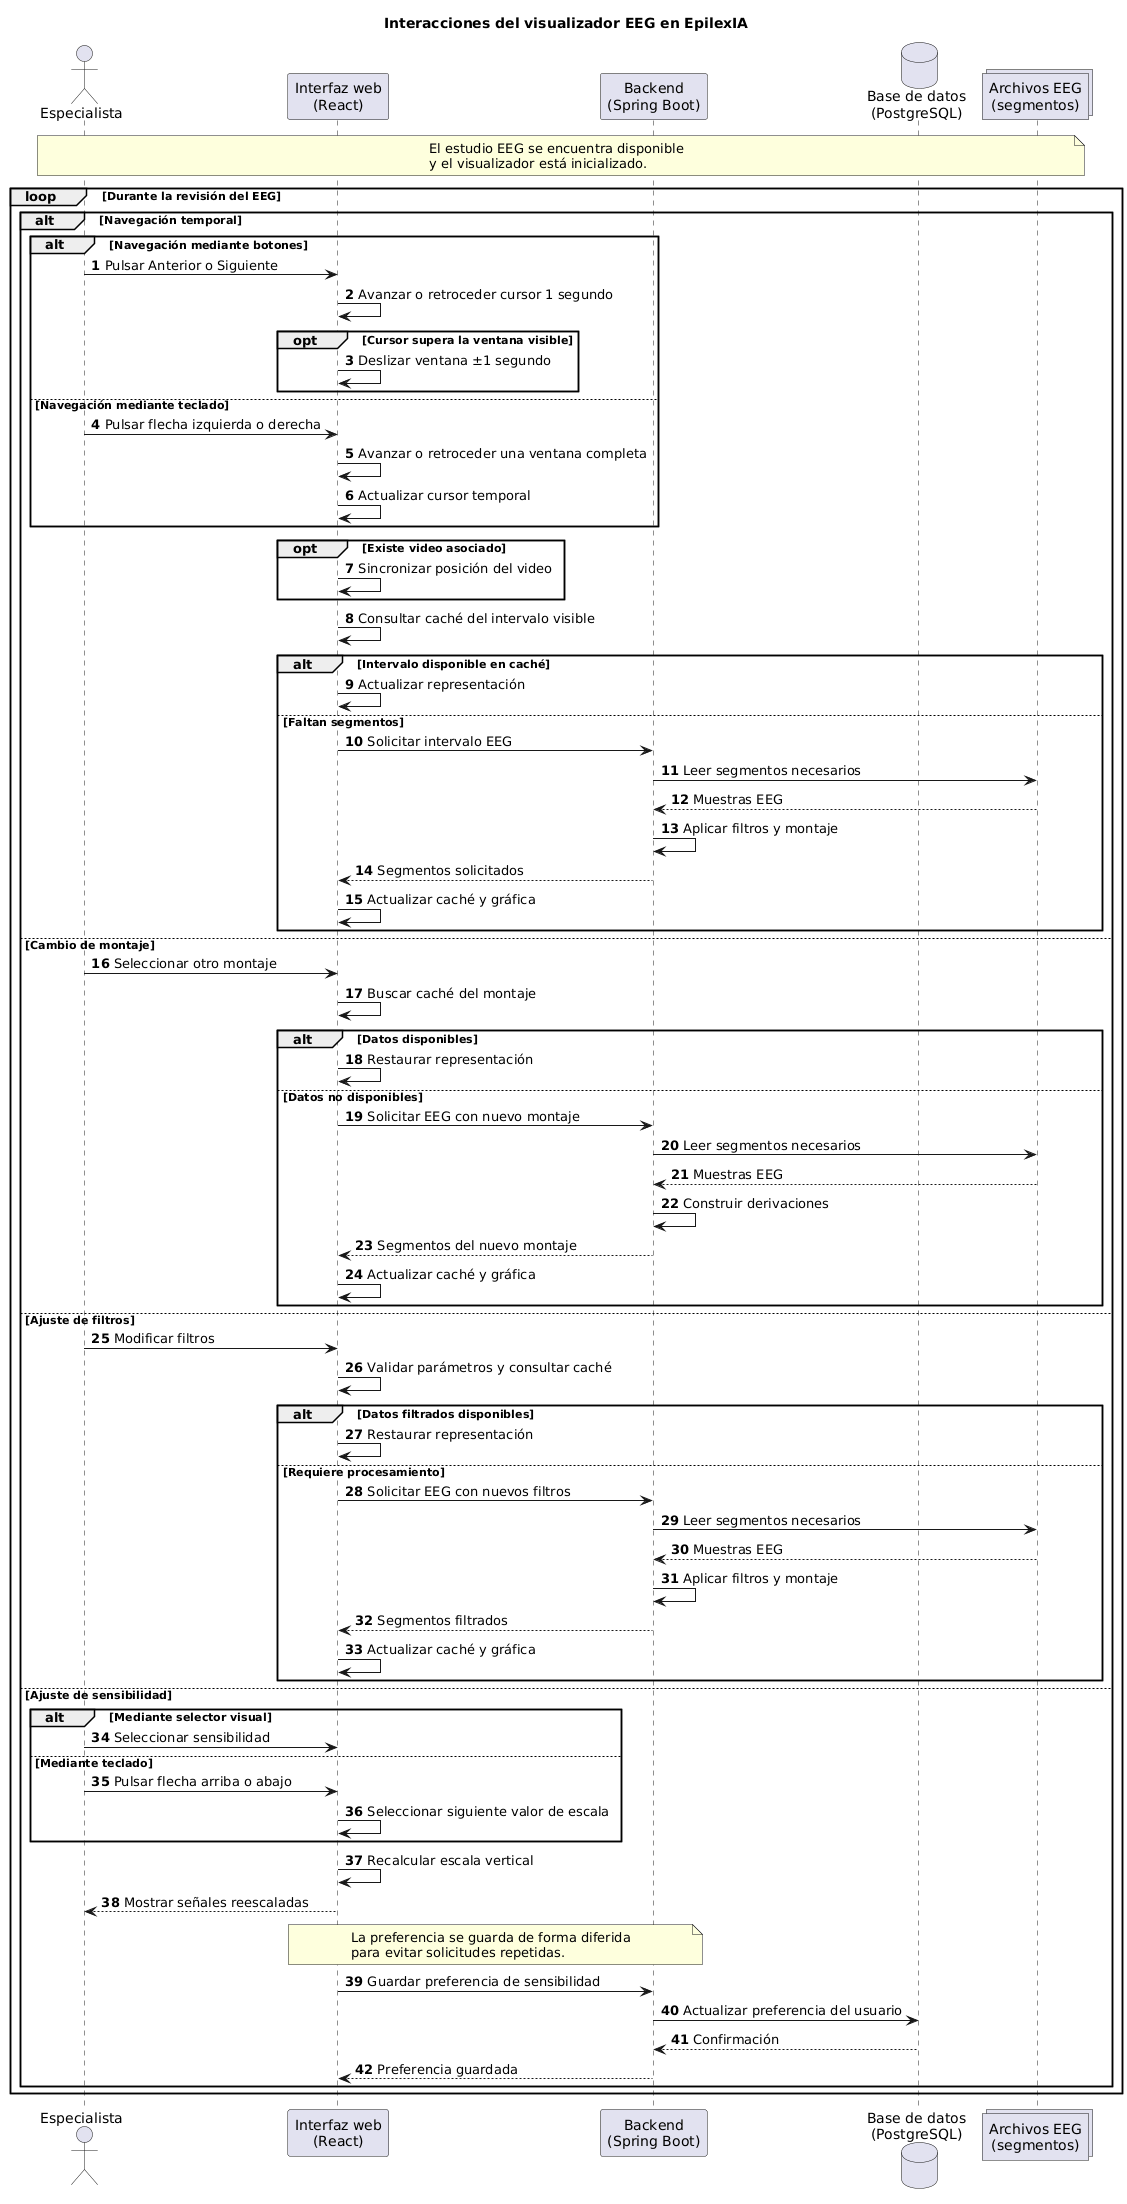
\includegraphics[
        width=\textwidth,
        height=0.82\textheight,
        keepaspectratio
    ]{ThesisFigs/secuencia_interacciones_visualizador_eeg.png}
    \caption{Diagrama de secuencia de las interacciones
    del visualizador EEG en EpilexIA.
    Elaboración propia.}
    \label{fig:secuencia-interacciones-visualizador-eeg}
\end{figure}


\subsection{Procesamiento de estudios mediante inteligencia artificial}
\label{subsec:secuencia-procesamiento-ia}

El procesamiento de estudios EEG mediante inteligencia
artificial constituye una funcionalidad de apoyo al
análisis realizado por el Especialista. Este proceso
permite solicitar el análisis automatizado de un
registro electroencefalográfico y consultar los
resultados obtenidos mediante el servicio de IA
integrado en EpilexIA.

La solicitud se origina en la interfaz web y es
recibida por el \textit{backend} principal, que verifica
los permisos del usuario, las condiciones del
estudio y la disponibilidad del archivo EEG.
Cuando se cumplen las condiciones necesarias,
el \textit{backend} se comunica con la API de IA para
solicitar el procesamiento.

Antes de iniciar una nueva ejecución, el sistema
comprueba si existe una ejecución activa que pueda
ser reutilizada. Cuando corresponde iniciar un
nuevo procesamiento, la API de IA registra la
ejecución y devuelve su identificador y estado
inicial. El \textit{backend} conserva la referencia
correspondiente para permitir su seguimiento.

La Figura~\ref{fig:secuencia-solicitud-ia}
presenta las principales interacciones relacionadas
con la solicitud y el registro de una ejecución
de procesamiento mediante IA.

\begin{figure}[H]
    \centering
    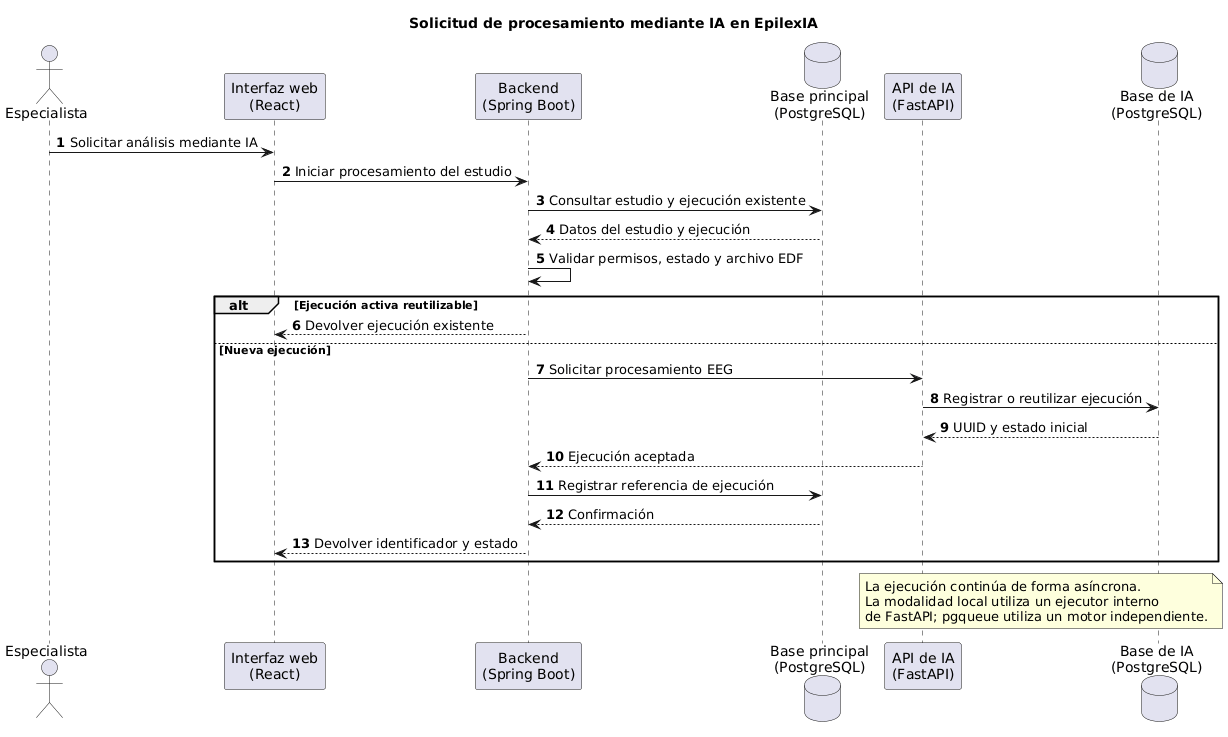
\includegraphics[
        width=\textwidth,
        height=0.82\textheight,
        keepaspectratio
    ]{ThesisFigs/secuencia_solicitud_ia.png}
    \caption{Diagrama de secuencia de la solicitud
    de procesamiento mediante inteligencia artificial
    en EpilexIA. Elaboración propia.}
    \label{fig:secuencia-solicitud-ia}
\end{figure}

El procesamiento se desarrolla de manera asíncrona,
por lo que la aceptación de una solicitud no implica
que el análisis haya finalizado. La ejecución se realiza a través de un motor independiente que obtiene
los trabajos desde una cola persistente.

Durante el procesamiento, la interfaz web consulta
periódicamente el estado de la ejecución. El \textit{backend}
obtiene la información correspondiente y, cuando
resulta necesario, consulta el estado actualizado
mediante la API de IA. Este mecanismo permite
identificar la finalización satisfactoria del
procesamiento o la ocurrencia de errores.

Una vez completada correctamente la ejecución,
el sistema permite recuperar los resultados
almacenados por el servicio de IA y presentarlos
al Especialista. Una ejecución exitosa puede
producir una lista vacía de anomalías, lo que
indica que no se registraron resultados que
cumplieran los criterios de detección establecidos
para dicha ejecución.

La Figura~\ref{fig:secuencia-resultados-ia}
representa el seguimiento del procesamiento
y la posterior consulta de los resultados
obtenidos mediante inteligencia artificial.

\begin{figure}[H]
    \centering
    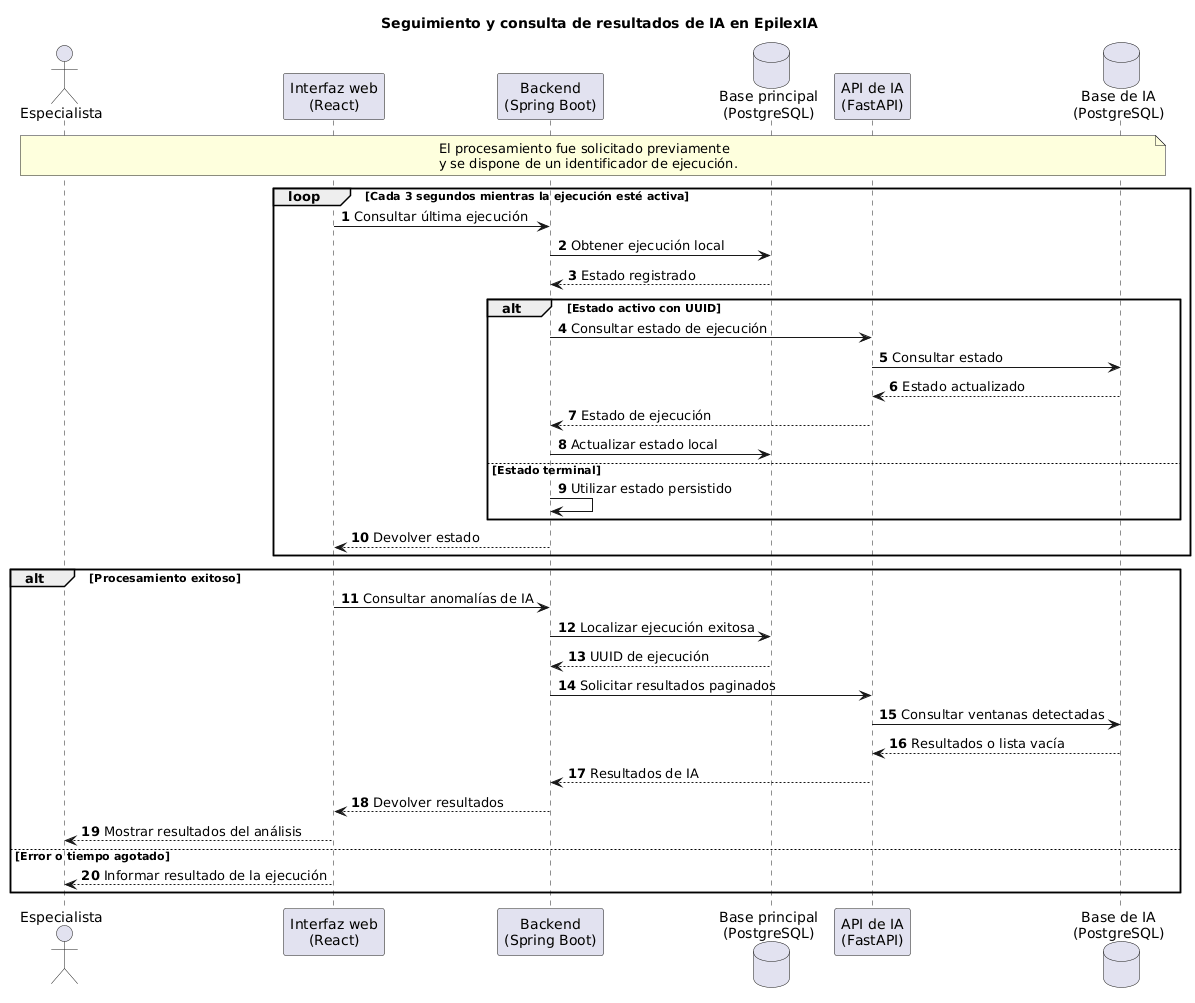
\includegraphics[
        width=\textwidth,
        height=0.82\textheight,
        keepaspectratio
    ]{ThesisFigs/secuencia_resultados_ia.png}
    \caption{Diagrama de secuencia del seguimiento
    y consulta de resultados de inteligencia
    artificial en EpilexIA. Elaboración propia.}
    \label{fig:secuencia-resultados-ia}
\end{figure}

Los resultados obtenidos mediante IA constituyen
información complementaria para la revisión
del estudio y se mantienen diferenciados de
las anotaciones manuales. Su interpretación
clínica corresponde al Especialista, por lo
que el procesamiento automatizado no sustituye
su criterio profesional.


\subsection{Elaboración y cierre de informes clínicos}
\label{subsec:secuencia-informes-clinicos}

La elaboración de informes clínicos constituye una
de las actividades principales realizadas por los
Especialistas durante la revisión de los estudios
electroencefalográficos. EpilexIA permite asociar
informes a un estudio EEG y mantener identificado
al profesional responsable de su elaboración.

El proceso comienza con la consulta de los informes
disponibles para el estudio. Un Especialista autorizado
puede acceder a los informes asociados y, cuando se
cumplen las condiciones correspondientes, crear
su propio informe. La creación genera un documento
en estado Borrador, inicialmente sin contenido clínico,
evitando que se reutilice información perteneciente
a informes elaborados por otros profesionales.

La Figura~\ref{fig:secuencia-creacion-informe}
presenta las interacciones involucradas en la
consulta y creación de informes clínicos.

\begin{figure}[H]
    \centering
    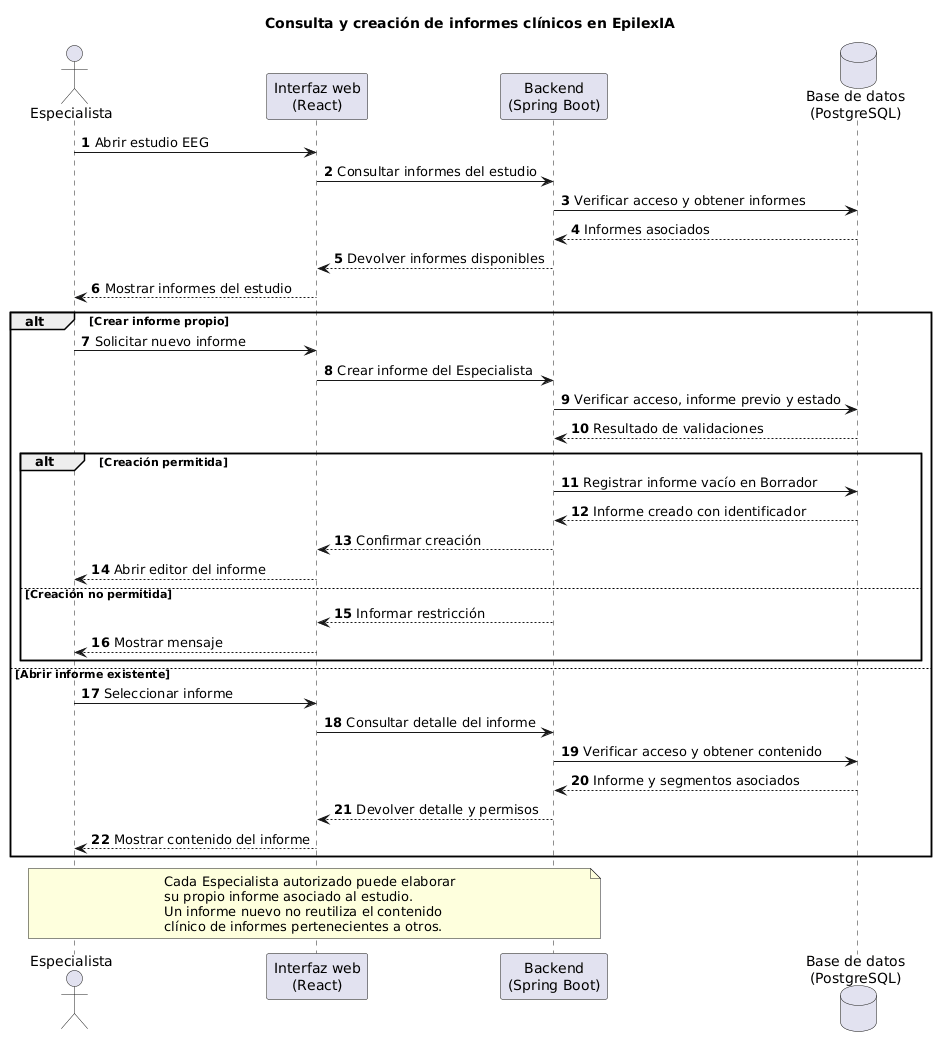
\includegraphics[
        width=\textwidth,
        height=0.82\textheight,
        keepaspectratio
    ]{ThesisFigs/secuencia_creacion_informe.png}
    \caption{Diagrama de secuencia de la consulta
    y creación de informes clínicos en EpilexIA.
    Elaboración propia.}
    \label{fig:secuencia-creacion-informe}
\end{figure}

Durante la elaboración del informe, el Especialista
puede completar la información clínica correspondiente
e incorporar segmentos de interés identificados
durante la revisión del estudio EEG. Estos segmentos
pueden proceder de anotaciones manuales o de
resultados obtenidos mediante el procesamiento
por inteligencia artificial.

Las modificaciones realizadas se envían al \textit{backend},
donde se verifican las condiciones necesarias para
autorizar la actualización. Entre estas condiciones
se encuentran la identificación del propietario
del informe y su estado. De esta manera, el sistema
diferencia la edición del informe propio de la
consulta de documentos pertenecientes a otros
profesionales.

La Figura~\ref{fig:secuencia-edicion-informe}
representa las principales interacciones relacionadas
con la edición y actualización de informes clínicos.

\begin{figure}[H]
    \centering
    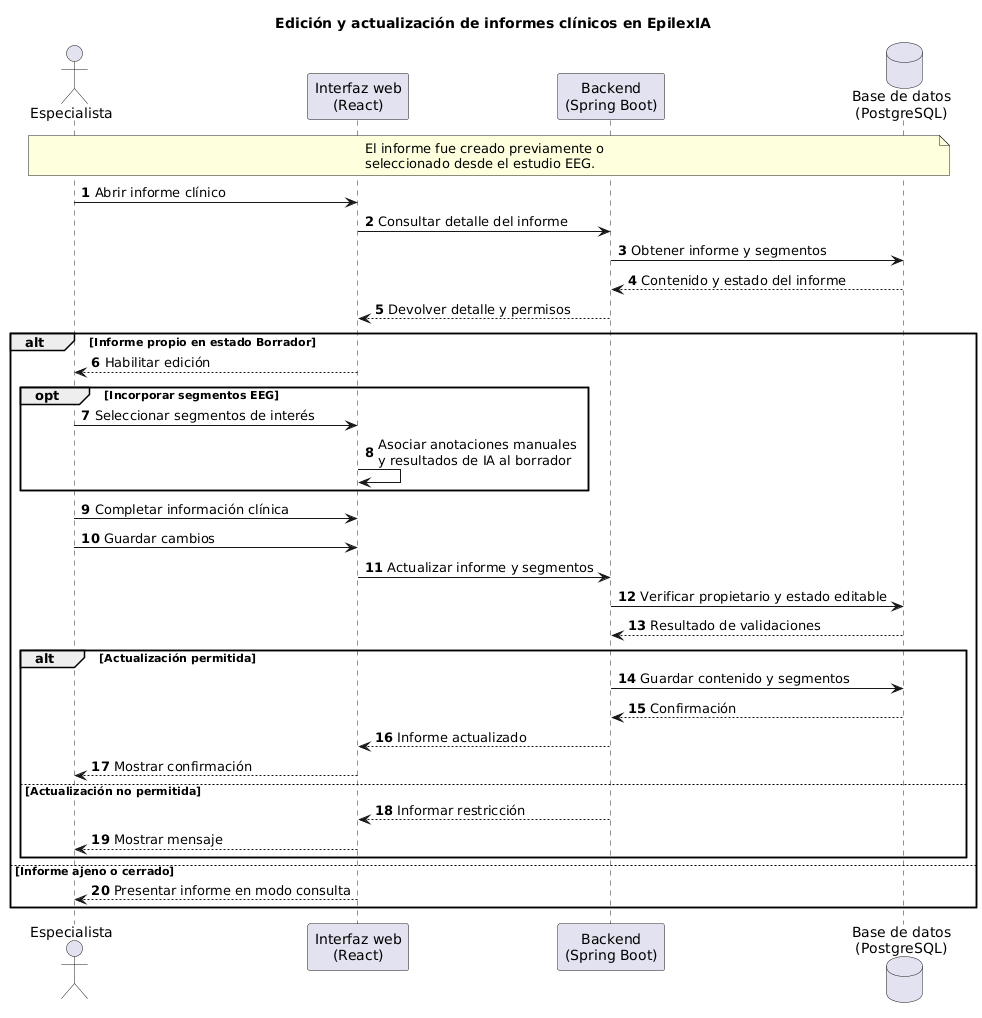
\includegraphics[
        width=\textwidth,
        height=0.82\textheight,
        keepaspectratio
    ]{ThesisFigs/secuencia_edicion_informe.png}
    \caption{Diagrama de secuencia de la edición
    y actualización de informes clínicos en EpilexIA.
    Elaboración propia.}
    \label{fig:secuencia-edicion-informe}
\end{figure}

Una vez finalizada la elaboración del informe,
el Especialista responsable puede solicitar su cierre.
Esta operación requiere una validación específica,
diferente de la utilizada para guardar los cambios
durante la edición. Cuando se cumplen las condiciones establecidas, el sistema actualiza el informe al estado Cerrado y registra la fecha y hora correspondientes al cierre.

El cierre impide que el contenido clínico continúe
modificándose mediante el flujo ordinario de edición.
No obstante, el informe permanece disponible para
su consulta por parte de los usuarios autorizados.

Asimismo, EpilexIA permite generar una representación
del informe en formato PDF. Esta operación recupera
la información clínica y los segmentos asociados,
sin modificar el contenido del documento almacenado.

La Figura~\ref{fig:secuencia-cierre-informe}
presenta las interacciones correspondientes al
cierre y posterior consulta de informes clínicos.

\begin{figure}[H]
    \centering
    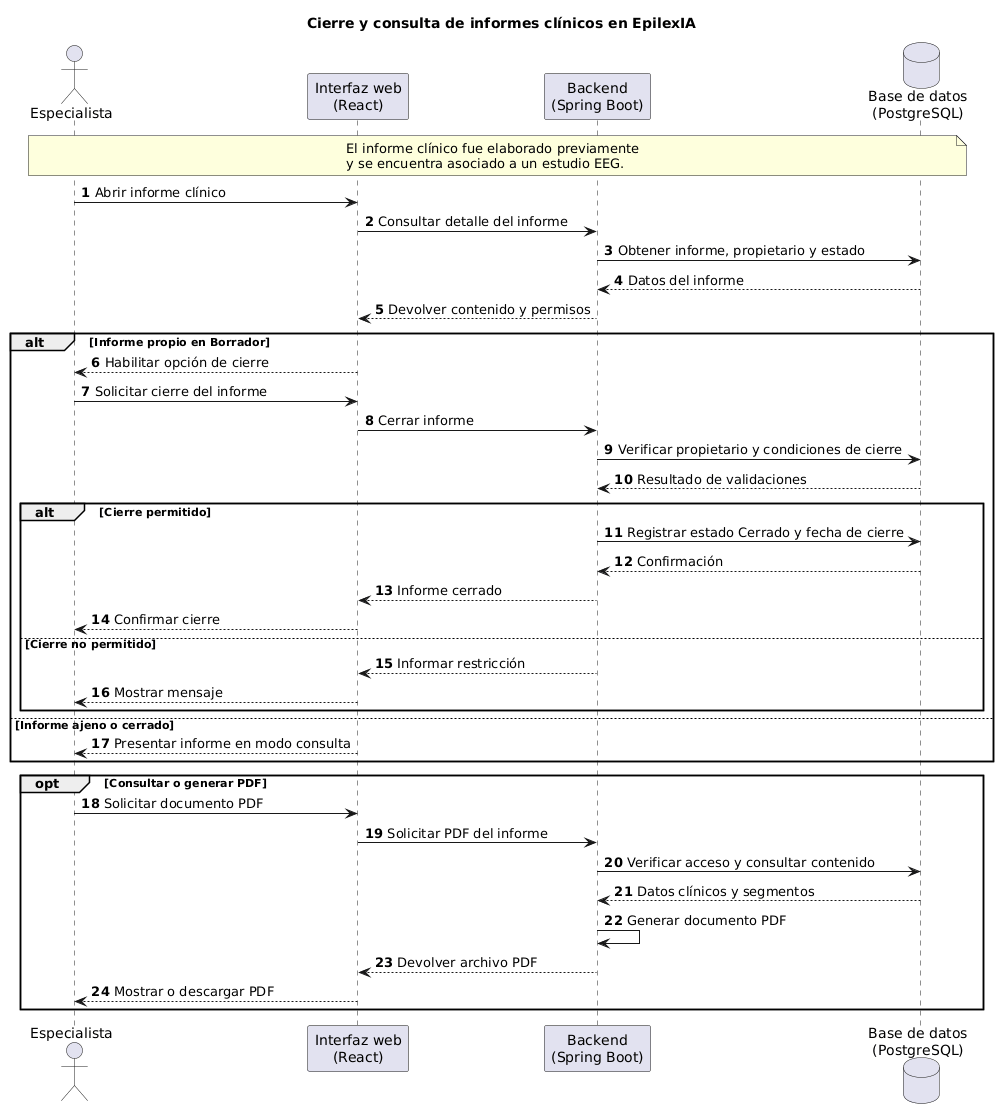
\includegraphics[
        width=\textwidth,
        height=0.82\textheight,
        keepaspectratio
    ]{ThesisFigs/secuencia_cierre_informe.png}
    \caption{Diagrama de secuencia del cierre
    y consulta de informes clínicos en EpilexIA.
    Elaboración propia.}
    \label{fig:secuencia-cierre-informe}
\end{figure}

La separación entre creación, edición y cierre
permite conservar la identificación del profesional
responsable, controlar las modificaciones y mantener
la disponibilidad de los informes asociados a un
mismo estudio. Estas características contribuyen
a la organización del trabajo clínico y a la
trazabilidad de la información registrada.


\section{Arquitectura del sistema}
\label{sec:arquitectura-sistema}

La arquitectura de EpilexIA fue diseñada con el propósito de organizar
las funcionalidades del sistema en componentes diferenciados, de acuerdo
con sus responsabilidades dentro del proceso de gestión y análisis de
estudios electroencefalográficos.

La solución adopta una arquitectura web en la que se separan la
interfaz de usuario, la lógica de negocio, la persistencia de la
información y el procesamiento mediante inteligencia artificial.
Esta organización permite que los componentes se comuniquen mediante
interfaces definidas, manteniendo diferenciadas las operaciones
relacionadas con la gestión clínica y aquellas destinadas al
procesamiento automatizado de las señales EEG.

El diseño contempla la interacción entre los usuarios y la aplicación
web, la administración de la información asociada con pacientes y
estudios, el acceso a los archivos electroencefalográficos y la
integración de los resultados generados mediante inteligencia
artificial.

\subsection{Arquitectura general}
\label{subsec:arquitectura-general}

EpilexIA se organiza mediante una arquitectura cliente-servidor,
complementada con componentes especializados para el procesamiento
de señales EEG.

La interfaz web constituye el punto de acceso de los usuarios
autorizados. Desde ella se realizan las operaciones relacionadas
con la administración del sistema, la gestión de estudios, la
visualización de señales electroencefalográficas y la elaboración
de informes clínicos.

Las solicitudes realizadas desde la interfaz son atendidas por
el \textit{backend} principal, encargado de aplicar las reglas de negocio,
verificar las condiciones de acceso y coordinar las operaciones
necesarias para consultar o modificar la información almacenada.

La persistencia de la información estructurada se organiza mediante dos bases de datos PostgreSQL: una destinada a la gestión clínica y administrativa del sistema, y otra utilizada por el subsistema de inteligencia artificial para almacenar información relacionada con las ejecuciones y sus resultados. Por otra parte, los archivos asociados con los estudios EEG se conservan mediante mecanismos de almacenamiento independientes de las estructuras relacionales.

Para incorporar el análisis automatizado de las señales,
la arquitectura incluye un servicio de inteligencia artificial
integrado mediante una interfaz de programación de aplicaciones.
Este servicio permite gestionar las solicitudes de procesamiento
y consultar los resultados producidos por el componente de análisis.

La arquitectura también contempla la separación entre la
gestión de las ejecuciones de inteligencia artificial y el
procesamiento de las señales. De esta manera, las operaciones
de gestión clínica permanecen diferenciadas de las tareas
computacionales requeridas para el análisis automatizado.

%La Figura~\ref{fig:arquitectura-general} presenta la
%organización general de estos componentes y sus principales
%relaciones.
La Figura~\ref{fig:arquitectura-general} presenta la arquitectura general del sistema EpilexIA, organizada en componentes con responsabilidades diferenciadas. La capa de presentación proporciona la interfaz mediante la cual los usuarios autorizados interactúan con el sistema, mientras que la capa de aplicación concentra las reglas de negocio y coordina las operaciones relacionadas con la gestión de pacientes, estudios electroencefalográficos e informes clínicos.

La persistencia principal comprende los repositorios destinados al almacenamiento de información clínica y administrativa, así como los archivos asociados a los estudios EEG y sus registros de video.

Por su parte, el subsistema de inteligencia artificial dispone de un servicio encargado de recibir y gestionar las solicitudes de análisis, administrar las ejecuciones y proporcionar acceso a los resultados obtenidos. Para la detección automática de crisis epilépticas, las tareas de análisis se registran en una cola persistente y son procesadas por un motor independiente.


En la configuración actualmente utilizada, el procesamiento destinado a la detección automática de crisis epilépticas se encuentra asignado al motor independiente. La coordinación entre este componente y el servicio de IA se establece mediante un repositorio compartido, diseñado para administrar las tareas pendientes, registrar los estados de ejecución y almacenar los resultados del análisis. Por otra parte, la arquitectura contempla la generación de espectrogramas DSA directamente en el servicio de IA, de forma independiente de la detección de crisis.


Esta organización establece una separación de responsabilidades entre los componentes del sistema y permite identificar los mecanismos de integración de la plataforma web con los servicios de inteligencia artificial, sin vincular la representación arquitectónica con tecnologías específicas de implementación. En este contexto, el presente trabajo de tesis se centra en el desarrollo de la plataforma web y en la integración del subsistema de inteligencia artificial, mientras que el desarrollo y el entrenamiento de los modelos de detección, a cargo del equipo de ciencia de datos, y la infraestructura tecnológica forman parte del proyecto integral EpilexIA.


\begin{figure}[H]
    \centering
    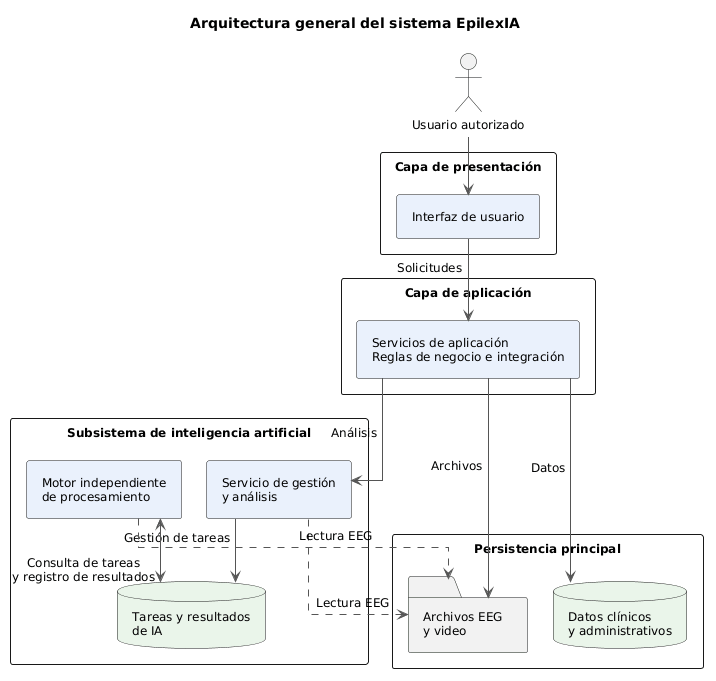
\includegraphics[width=\textwidth]{ThesisFigs/arquitectura_general_epilexia.png}
    \caption{Arquitectura general del sistema EpilexIA.
    Elaboración propia.}
    \label{fig:arquitectura-general}
\end{figure}


\subsection{Componentes de la arquitectura}
\label{subsec:componentes-arquitectura}

La arquitectura de EpilexIA está conformada por componentes
que cumplen responsabilidades específicas dentro del sistema.
Su organización permite separar las operaciones realizadas
por los usuarios, la gestión de la información clínica, el
almacenamiento de archivos y el procesamiento automatizado
de señales EEG.

Como se observa en la Figura~\ref{fig:arquitectura-general},
los componentes principales se distribuyen entre la capa
de presentación, la capa de aplicación, la persistencia
de datos y archivos, y el subsistema de inteligencia
artificial.

\subsubsection{Capa de presentación}

La capa de presentación corresponde a la interfaz web
desarrollada con React y TypeScript. Constituye el punto
de interacción entre los usuarios autorizados y las
funcionalidades disponibles en EpilexIA.

Este componente permite acceder a las operaciones de administración, gestionar la información de pacientes en el contexto de los estudios EEG, visualizar las señales electroencefalográficas, consultar los resultados del procesamiento mediante inteligencia artificial y elaborar informes clínicos.

La interfaz organiza las funcionalidades disponibles de
acuerdo con los permisos del usuario autenticado y
se comunica con el \textit{backend} principal mediante solicitudes
a una API REST.

\subsubsection{Capa de aplicación}

La capa de aplicación está representada por el \textit{backend} principal, desarrollado en Java mediante Spring Boot y preparado para su despliegue como una aplicación WAR sobre el servidor de aplicaciones WildFly.

Este componente concentra las reglas de negocio
relacionadas con la gestión de usuarios, pacientes,
estudios EEG, informes clínicos y eventos de auditoría.
Asimismo, verifica las condiciones de autorización
necesarias para ejecutar las operaciones solicitadas
desde la interfaz web.

El \textit{backend} también coordina el acceso a los datos
persistentes, la gestión de los archivos asociados
con los estudios y la comunicación con el servicio
de inteligencia artificial.

Esta organización permite mantener las validaciones
y las reglas de acceso en el servidor, independientemente
de los controles disponibles en la interfaz de usuario.

\subsubsection{Persistencia de datos y archivos}

La arquitectura contempla mecanismos diferenciados
para almacenar la información estructurada del sistema
y los archivos utilizados durante el análisis de los
estudios EEG.

La base de datos principal, implementada mediante
PostgreSQL, almacena la información correspondiente
a usuarios, pacientes, estudios, informes clínicos,
permisos y registros de auditoría, así como las
relaciones necesarias entre estas entidades.

Por otra parte, los archivos asociados con los
estudios, como los registros electroencefalográficos
y los videos, se conservan mediante mecanismos
de almacenamiento de archivos.

Esta separación permite que la base de datos
mantenga las referencias y los metadatos necesarios
para relacionar los archivos con los estudios,
sin incorporar directamente su contenido completo
a las estructuras relacionales.

\subsubsection{Subsistema de inteligencia artificial}

El subsistema de inteligencia artificial constituye
un conjunto de componentes especializados que
permiten incorporar el procesamiento automatizado
de señales EEG al funcionamiento de EpilexIA.


La comunicación con este subsistema se realiza mediante una API desarrollada con FastAPI, que recibe las solicitudes provenientes del \textit{backend} principal y proporciona los mecanismos necesarios para consultar el estado de las ejecuciones y recuperar los resultados almacenados. La arquitectura contempla, además, la ejecución de nuevas tareas de procesamiento mediante los componentes especializados del subsistema.


El subsistema dispone de una base de datos
PostgreSQL destinada a gestionar la información
relacionada con las ejecuciones de procesamiento
y sus resultados.

Las solicitudes pendientes se gestionan mediante una cola persistente en la base de datos de IA, denominada \texttt{pgqueue}, y son atendidas por un motor de procesamiento independiente.


La arquitectura tiene como propósito facilitar la recuperación y consulta de los resultados obtenidos mediante inteligencia artificial, de manera que puedan utilizarse como información complementaria durante la revisión de los estudios EEG.  La verificación del ciclo completo, desde la solicitud del análisis hasta la presentación de nuevos resultados, se documenta en el Capítulo~\ref{pruebas_evaluacion}.


El desarrollo y entrenamiento del modelo de
inteligencia artificial no forman parte del alcance
de este trabajo, cuya participación
se concentra en su integración con los componentes
del sistema y en la presentación de los resultados
para su revisión por parte del Especialista.


\subsection{Comunicación entre componentes}
\label{subsec:comunicacion-componentes}

La comunicación entre los componentes de EpilexIA se
organiza a partir de las solicitudes realizadas por
los usuarios mediante la interfaz web. Estas solicitudes
son atendidas por el \textit{backend} principal, que coordina
las operaciones necesarias y establece la comunicación
con los mecanismos de persistencia y los servicios
especializados del sistema.

La interacción entre la capa de presentación y la
capa de aplicación se realiza mediante una API REST.
A través de esta interfaz, el \textit{frontend} envía las
solicitudes relacionadas con la autenticación,
la gestión de pacientes y estudios EEG, la consulta
de señales electroencefalográficas y la elaboración
de informes clínicos.

El \textit{backend} recibe estas solicitudes, verifica las
condiciones de acceso correspondientes y ejecuta
las reglas de negocio asociadas con cada operación.
Posteriormente, devuelve las respuestas necesarias
para que la interfaz actualice la información
presentada al usuario.

Para las operaciones que requieren información
persistente, el \textit{backend} interactúa con la base
de datos principal PostgreSQL. Esta comunicación
permite consultar y actualizar los registros
relacionados con usuarios, pacientes, estudios,
informes y eventos de auditoría.

En el caso de los archivos asociados con los
estudios EEG, el \textit{backend} coordina las operaciones
de almacenamiento y recuperación de los datos
necesarios para su posterior procesamiento
y visualización. La información estructurada
que identifica y relaciona estos archivos
con los estudios se conserva en la base de
datos principal.

La comunicación con el subsistema de inteligencia
artificial se establece mediante la API desarrollada
con FastAPI. Cuando se solicita el procesamiento
automatizado de un estudio, el \textit{backend} principal
verifica las condiciones necesarias y transmite
la solicitud al servicio de IA.


La arquitectura contempla el procesamiento asíncrono de las solicitudes de análisis, de manera que la operación inicial no requiera mantener al usuario esperando hasta la finalización del procesamiento. Para ello, se dispone de mecanismos destinados a consultar el estado de las ejecuciones y recuperar los resultados almacenados cuando estén disponibles.


Dentro del subsistema de IA, las ejecuciones pendientes son atendidas por un motor independiente
que utiliza la base de datos de IA para gestionar
los trabajos y registrar sus resultados.


Los resultados de inteligencia artificial almacenados pueden recuperarse mediante la comunicación entre el \textit{backend} principal y la API de IA. Posteriormente, la interfaz web permite presentarlos en el contexto del estudio correspondiente, de manera que el Especialista pueda examinarlos junto con las señales EEG. Este mecanismo contempla tanto la consulta de resultados existentes como la recuperación de nuevos resultados cuando finalicen las ejecuciones de procesamiento.


Esta organización permite mantener una
comunicación diferenciada entre los componentes
encargados de la gestión del sistema y aquellos
destinados al procesamiento automatizado,
conservando al \textit{backend} principal como punto
de coordinación de las operaciones solicitadas
desde la interfaz web.


\section{Diseño de la base de datos}
\label{sec:diseno-base-datos}

El diseño de persistencia de EpilexIA contempla
la separación de la información clínica y operativa
del sistema respecto de los datos utilizados para
coordinar el procesamiento mediante inteligencia
artificial. Para ello, se emplean dos bases de datos
relacionales PostgreSQL, con responsabilidades
diferenciadas.

\subsection{Organización general de los datos}
\label{subsec:organizacion-datos}

La base de datos principal almacena la información
estructurada necesaria para la gestión de usuarios,
pacientes, estudios EEG, informes médicos, anomalías
registradas y demás operaciones de la plataforma.
Esta información permite establecer las relaciones
entre los estudios y los profesionales que intervienen
en su registro, revisión e interpretación.

Por otra parte, el subsistema de inteligencia artificial
dispone de una base de datos independiente, destinada
a gestionar las solicitudes de procesamiento, sus
estados de ejecución y los resultados obtenidos.
Esta base de datos permite coordinar las actividades
entre la API de inteligencia artificial y el motor
de procesamiento.

Los archivos que contienen las señales EEG y los
videos asociados se conservan en un almacenamiento
de archivos independiente de las tablas relacionales.
De esta manera, la información estructurada del
sistema puede relacionarse con los registros
electroencefalográficos sin requerir que el contenido
completo de dichos archivos se almacene directamente
en la base de datos clínica.


\subsection{Modelo de datos clínicos}
\label{subsec:modelo-datos-clinicos}

El modelo de datos clínicos de EpilexIA se estructura
principalmente alrededor de las entidades
\texttt{patient} y \texttt{study}, que representan,
respectivamente, a los pacientes registrados y sus
estudios electroencefalográficos. La relación entre
ambas entidades es de uno a muchos, dado que un
paciente puede tener varios estudios EEG, mientras
que cada estudio corresponde a un único paciente.

La entidad \texttt{study} constituye el núcleo del modelo y mantiene referencias a los usuarios que intervienen en la gestión del estudio. Cada estudio debe estar asociado obligatoriamente a un usuario responsable, cuya pertenencia al rol Especialista se verifica mediante las reglas de negocio del \textit{backend} durante su creación. Asimismo, puede incluir de manera opcional un técnico encargado de su registro. La entidad también conserva información sobre el estado del estudio, su anulación, reactivación y disponibilidad de video.

Los archivos asociados a cada estudio se representan mediante la entidad
\texttt{study\_file}, relacionada con el catálogo
\texttt{study\_file\_type}, que permite identificar el formato
correspondiente. Esta estructura admite múltiples archivos por estudio,
incluyendo señales EEG y videos, y conserva metadatos técnicos como la
duración, la frecuencia de muestreo y los canales disponibles.
Estos metadatos se registran o completan durante las operaciones de carga
y procesamiento de los archivos, de acuerdo con las características y
los mecanismos de lectura de cada formato.

Para representar las configuraciones de visualización,
el modelo incorpora las entidades \texttt{eeg\_montage}
y \texttt{eeg\_montage\_channel}. La primera define los
montajes electroencefalográficos disponibles, mientras
que la segunda establece los canales o derivaciones
que componen cada montaje y su orden de presentación.

Los hallazgos registrados durante la revisión de un
estudio se organizan en dos estructuras diferenciadas.
La entidad \texttt{anomaly} representa intervalos de
señal identificados manualmente o mediante inteligencia
artificial, con referencias opcionales a su clasificación
y montaje. Por otra parte, \texttt{study\_eeg\_event}
almacena eventos temporales asociados al estudio,
utilizando tipos predefinidos o personalizados.


La elaboración de informes médicos se modela mediante las entidades \texttt{report}, \texttt{study\_report} y \texttt{report\_segment}. La entidad \texttt{report} almacena el contenido clínico del informe, mientras que \texttt{study\_report} establece la asociación entre el estudio, el Especialista y el informe correspondiente. Esta relación permite la existencia de informes elaborados por diferentes Especialistas para un mismo estudio, con la restricción de un único informe por Especialista dentro de dicho estudio.


Finalmente, \texttt{report\_segment} permite asociar
a cada informe los intervalos de señal considerados
relevantes, conservando información sobre su ubicación
temporal y, cuando corresponde, sus referencias a
anomalías, montajes o ejecuciones de inteligencia
artificial.

El modelo se complementa con estructuras de control
de acceso, compartición de estudios y auditoría,
que permiten relacionar las operaciones clínicas con
los usuarios participantes y conservar información
para su trazabilidad.


La Figura~\ref{fig:er-pacientes-estudios}
presenta las principales entidades relacionadas
con el registro de pacientes, la gestión de estudios
electroencefalográficos, sus archivos asociados
y las configuraciones de montaje EEG.

Por su parte, la Figura~\ref{fig:er-informes-anomalias}
representa las relaciones entre los estudios,
las anomalías, los eventos EEG y los informes
clínicos elaborados por los especialistas.
Ambas figuras constituyen vistas simplificadas
del modelo relacional, en las que se priorizan
las entidades y asociaciones más relevantes
para comprender el diseño del sistema.


\begin{figure}[H]
    \centering
    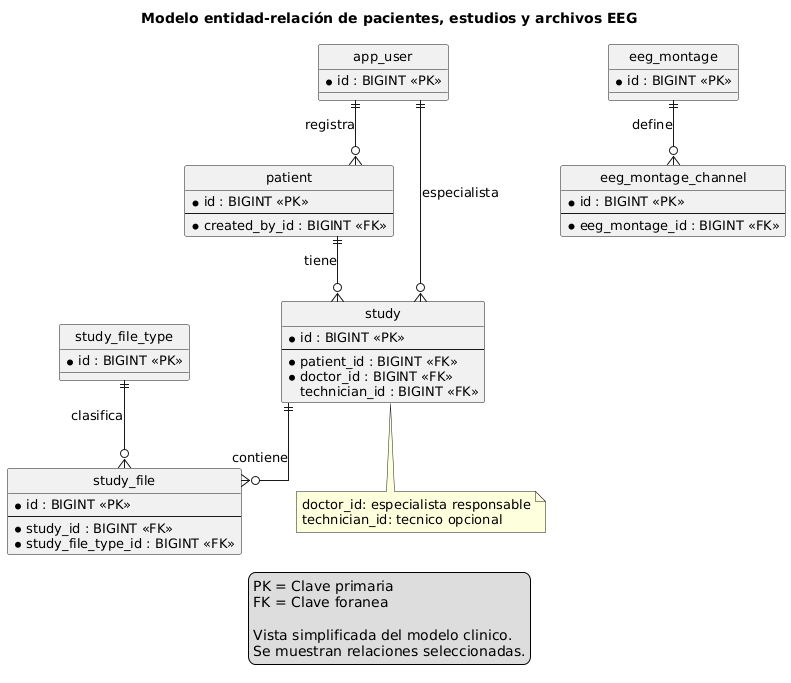
\includegraphics[width=\textwidth]{ThesisFigs/er_pacientes_estudios.png}
    \caption{Modelo entidad-relación de pacientes,
    estudios y archivos EEG de EpilexIA.}
    \label{fig:er-pacientes-estudios}
\end{figure}

\begin{figure}[H]
    \centering
    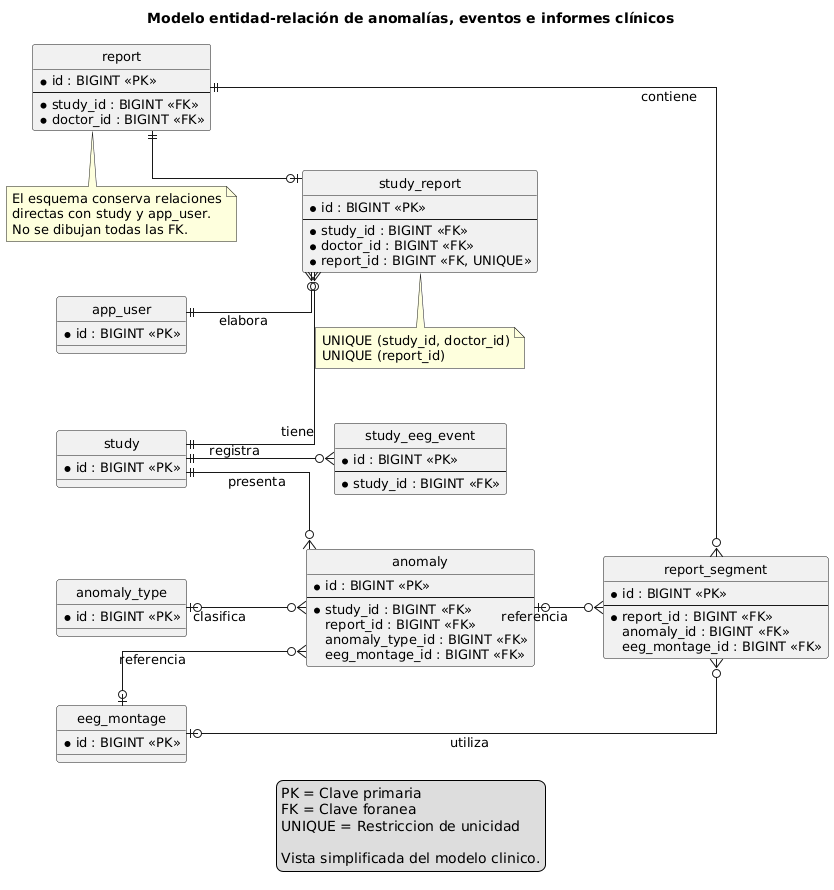
\includegraphics[width=\textwidth]{ThesisFigs/er_informes_anomalias.png}
    \caption{Modelo entidad-relación de anomalías,
    eventos e informes clínicos de EpilexIA.}
    \label{fig:er-informes-anomalias}
\end{figure}


\subsection{Modelo de datos del procesamiento de inteligencia artificial}
\label{subsec:modelo-datos-ia}

El subsistema de inteligencia artificial de EpilexIA utiliza una base de datos PostgreSQL independiente de la base de datos clínica principal. Su diseño permite registrar las solicitudes de procesamiento de señales EEG, controlar los estados de ejecución, almacenar los resultados obtenidos y conservar información de retroalimentación proporcionada por los especialistas. El esquema comprende seis tablas principales, cuya estructura es administrada mediante migraciones de la API de inteligencia artificial desarrollada con FastAPI.

La entidad central del modelo es \texttt{ai\_executions}, que representa cada solicitud de análisis electroencefalográfico. Cada ejecución se identifica mediante un UUID y conserva información sobre el estudio asociado, el modelo utilizado, su versión, el umbral mínimo de probabilidad y la ubicación del archivo EEG que debe procesarse. Asimismo, registra el estado de ejecución, las fechas de inicio y finalización y los datos operativos necesarios para identificar posibles errores.

El ciclo de vida de una ejecución se representa mediante estados como \texttt{QUEUED}, \texttt{RUNNING}, \texttt{SUCCESS}, \texttt{FAILED}, \texttt{TIMEOUT} y \texttt{CANCELLED}. Adicionalmente, el subsistema contempla el estado interno \texttt{CANCEL\_REQUESTED}, utilizado para coordinar las solicitudes de cancelación durante el procesamiento mediante cola.

La configuración del modelo activo se administra mediante la entidad \texttt{ai\_model\_params}, que almacena parámetros como el nombre, la versión y el umbral mínimo de probabilidad de crisis. Al registrar una ejecución, estos valores se incorporan a \texttt{ai\_executions}, permitiendo conservar la configuración utilizada en cada procesamiento. Los archivos que contienen los modelos entrenados se mantienen fuera de la base de datos, en un almacenamiento independiente.

Los resultados del análisis se representan mediante la entidad \texttt{ai\_results}, relacionada con \texttt{ai\_executions} mediante una clave foránea. Cada registro corresponde a un intervalo temporal identificado por el procesamiento de inteligencia artificial y conserva su instante inicial, instante final y probabilidad estimada de crisis. El sistema almacena únicamente las ventanas clasificadas positivamente que cumplen el umbral mínimo configurado. Por consiguiente, una ejecución finalizada correctamente puede no generar registros de resultados cuando no se identifican intervalos que satisfagan dicho criterio.

El modelo incorpora mecanismos para conservar la revisión realizada por los especialistas. La entidad \texttt{ai\_results} dispone de atributos destinados a registrar la validación médica de los intervalos detectados. Por su parte, \texttt{ai\_report\_window\_inclusions} permite asociar los resultados de inteligencia artificial con los informes clínicos en los que fueron incluidos, conservando información descriptiva y de clasificación aportada por el profesional.

Complementariamente, la entidad \texttt{ai\_manual\_annotations} almacena anotaciones realizadas manualmente por los especialistas, incluso cuando no corresponden a intervalos detectados previamente por el modelo. Estas estructuras permiten conservar información de retroalimentación clínica que podría utilizarse en futuros procesos de mejora de los modelos de inteligencia artificial, sin que ello implique la existencia de un mecanismo automático de reentrenamiento en la implementación actual.

La base de datos también contempla la entidad \texttt{ai\_results\_historial}, destinada al almacenamiento histórico de resultados. Esta estructura se encuentra definida en el esquema; el traslado automático de registros hacia ella desde la tabla de resultados activos no está implementado en la versión actual.

La tabla \texttt{ai\_executions} cumple además una función de coordinación entre la API de inteligencia artificial y el motor de procesamiento independiente. La API registra las solicitudes pendientes y el motor adquiere los trabajos mediante operaciones transaccionales sobre PostgreSQL. Durante la ejecución se actualizan los estados y las señales de actividad del procesamiento, mientras que al finalizar se registran los resultados y el estado correspondiente.

La vinculación con la base de datos clínica se establece mediante identificadores compartidos a nivel de aplicación. En particular, \texttt{id\_study\_epilex} permite identificar el estudio clínico asociado, mientras que el UUID de la ejecución puede relacionarse con los registros de seguimiento mantenidos por el \textit{backend} principal. Debido a que ambas bases de datos funcionan de manera independiente, estas correspondencias no se implementan mediante claves foráneas entre ellas.

Finalmente, los archivos EEG, los modelos entrenados y los archivos temporales generados durante el procesamiento se conservan en almacenamiento de archivos. Esta separación permite mantener en PostgreSQL los datos estructurados necesarios para la gestión, consulta y trazabilidad de las ejecuciones, sin incorporar directamente los archivos de señales ni los artefactos del modelo.


La Figura~\ref{fig:er-subsistema-ia} presenta
una vista simplificada del modelo entidad-relación
del subsistema de inteligencia artificial de EpilexIA.
Se destacan las relaciones entre las ejecuciones
de procesamiento, los resultados generados y las
ventanas incorporadas a informes clínicos.
Asimismo, se representan las estructuras destinadas
a la configuración del modelo, las anotaciones
manuales y el almacenamiento histórico, diferenciando
las relaciones definidas mediante claves foráneas
de las referencias lógicas gestionadas por la aplicación.


\begin{figure}[H]
    \centering
    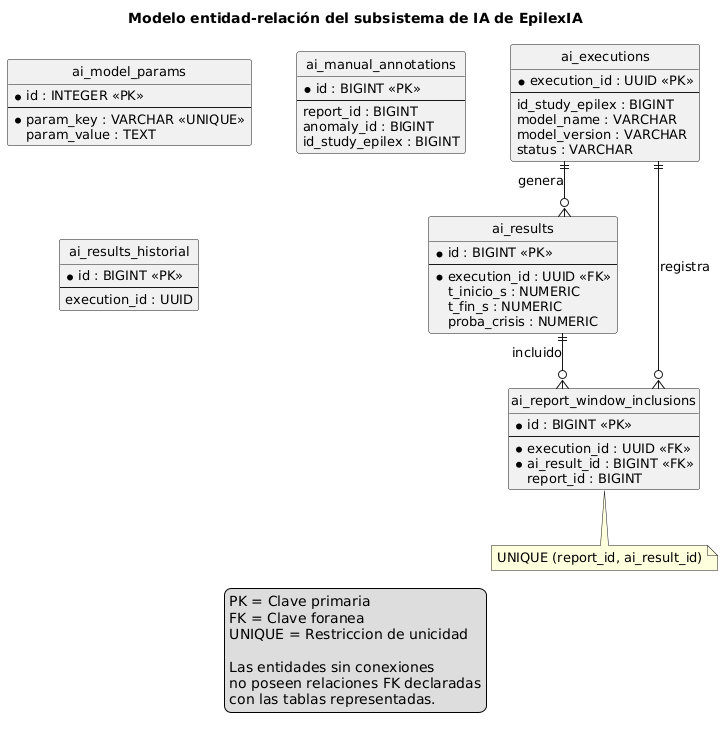
\includegraphics[width=\textwidth]{ThesisFigs/er_subsistema_ia.png}
    \caption{Modelo entidad-relación del subsistema
    de inteligencia artificial de EpilexIA.}
    \label{fig:er-subsistema-ia}
\end{figure}


\subsection{Integridad y persistencia de los datos}
\label{subsec:integridad-persistencia-datos}

El diseño de persistencia de EpilexIA contempla mecanismos
de integridad orientados a mantener la consistencia de
la información clínica y de los registros asociados al
procesamiento mediante inteligencia artificial. Para ello,
las bases de datos PostgreSQL emplean claves primarias,
claves foráneas y restricciones de unicidad que permiten
identificar los registros y controlar sus relaciones.

En la base de datos clínica, las restricciones de integridad
referencial permiten establecer asociaciones entre pacientes,
estudios electroencefalográficos, archivos, anomalías e
informes médicos. Estas relaciones contribuyen a evitar
referencias a registros inexistentes y a mantener la
correspondencia entre los estudios y la información generada
durante su revisión. Asimismo, determinadas restricciones
de unicidad permiten aplicar reglas del modelo, como la
existencia de un único informe por Especialista dentro
de un mismo estudio.

En la base de datos del subsistema de inteligencia artificial,
la integridad referencial se aplica principalmente a las
relaciones entre las ejecuciones de procesamiento, los
resultados obtenidos y los registros de inclusión de ventanas
en informes clínicos. Cada resultado se vincula con la
ejecución que lo generó, permitiendo identificar su origen
y conservar la trazabilidad de los intervalos detectados
por el modelo.

La separación entre la base de datos clínica y la base
de datos de inteligencia artificial implica que sus
correspondencias se gestionan mediante identificadores
compartidos a nivel de aplicación, sin establecer claves
foráneas entre ambas bases. De esta manera, cada subsistema
mantiene sus propias restricciones de integridad y
responsabilidades de persistencia.

Por otra parte, los archivos de señales EEG, los videos
asociados y los modelos entrenados se conservan en
almacenamiento de archivos, mientras que las bases de datos
mantienen los registros estructurados y las referencias
necesarias para su identificación y utilización. Esta
organización evita almacenar directamente archivos de gran
tamaño dentro de las tablas relacionales y permite separar
la gestión de metadatos del almacenamiento de los recursos
utilizados por el sistema.

Finalmente, el diseño incorpora registros de auditoría
y seguimiento de ejecuciones que contribuyen a la
trazabilidad de las operaciones realizadas. Estas
estructuras permiten relacionar las actividades registradas
con sus respectivos usuarios, estudios o procesos, según
corresponda, y proporcionan información para el análisis
de las operaciones del sistema.


\section{Diseño de los servicios e interfaces de integración}
\label{sec:diseno-servicios-integracion}

La integración de los componentes de EpilexIA se organiza
mediante interfaces de comunicación que permiten intercambiar
información entre la aplicación web, el \textit{backend} principal y
el subsistema de inteligencia artificial. Esta organización
establece responsabilidades diferenciadas para la gestión
clínica, el acceso a los estudios electroencefalográficos
y la ejecución de los procesos de análisis automatizado.

La interfaz web, desarrollada con React, consume los servicios
REST expuestos por el \textit{backend} principal, implementado con
Spring Boot y ejecutado sobre WildFly. Este componente
centraliza las operaciones relacionadas con usuarios,
pacientes, estudios EEG, informes médicos y auditoría,
además de gestionar la comunicación con los servicios
de inteligencia artificial.

La integración con el subsistema de inteligencia artificial
se realiza mediante una API independiente desarrollada
con FastAPI. El \textit{backend} principal utiliza esta interfaz
para solicitar análisis, consultar su estado, recuperar
resultados y obtener representaciones complementarias
de las señales EEG, como los espectrogramas.

La API de inteligencia artificial y el motor de procesamiento
se coordinan a través de una base de datos PostgreSQL
compartida por ambos componentes. Esta comunicación permite
gestionar las solicitudes de análisis sin requerir una
conexión HTTP directa entre la API y el motor.

El diseño de las interfaces también contempla mecanismos
de autenticación, validación de solicitudes y tratamiento
de errores, con el propósito de controlar el acceso a
las operaciones y proporcionar respuestas adecuadas
a los componentes consumidores.


\subsection{Servicios del \textit{backend} principal}
\label{subsec:servicios-backend-principal}

El \textit{backend} principal de EpilexIA constituye la capa
encargada de gestionar las operaciones del sistema y
coordinar el intercambio de información entre la interfaz
web, la base de datos clínica, el almacenamiento de
archivos y los servicios de inteligencia artificial.

Este componente fue desarrollado en Java, utilizando
Spring Boot y una arquitectura organizada en controladores
REST, servicios de aplicación y repositorios de
persistencia. Su despliegue se realiza mediante un
artefacto WAR preparado para ejecutarse sobre el
servidor de aplicaciones WildFly.

Los controladores exponen interfaces HTTP orientadas
a recursos, mediante las cuales el \textit{frontend} realiza
operaciones de consulta, registro, actualización y
gestión de información. Estas interfaces utilizan
principalmente mensajes en formato JSON y objetos
de transferencia de datos (DTO), que permiten
separar los contratos de comunicación de las
entidades utilizadas internamente por el sistema.

Los servicios REST se agrupan según sus
responsabilidades funcionales. Entre ellos se
encuentran la autenticación y administración de
usuarios, la gestión de pacientes y estudios EEG,
la recepción de archivos, la recuperación de señales
para su visualización, el registro de anomalías y
eventos, la elaboración de informes médicos y
la consulta de actividades de auditoría.

Para facilitar el intercambio de información,
la mayoría de las respuestas JSON emplea una
estructura común que identifica el resultado de
la operación, un mensaje opcional y los datos
solicitados. Asimismo, las consultas de listados
extensos incorporan mecanismos de paginación,
mientras que la transferencia de archivos utiliza
formatos adecuados a su naturaleza, como
\texttt{multipart/form-data} para las cargas
y respuestas binarias para los documentos generados.

La gestión de los estudios EEG contempla interfaces
para recibir archivos EDF mediante carga
fragmentada. Una vez completada la transferencia,
el \textit{backend} ensambla el archivo y ejecuta su
procesamiento de manera asíncrona. Como resultado,
se generan segmentos comprimidos que posteriormente
pueden recuperarse por índice o intervalo temporal.

Para la visualización de las señales, el \textit{backend}
proporciona servicios de consulta de metadatos,
segmentos, montajes y derivaciones. La resolución
de montajes y la aplicación de filtros digitales
se realizan en el servidor, mientras que la
sensibilidad seleccionada por el usuario interviene
en la representación gráfica efectuada por
la interfaz web.

La seguridad de estas interfaces combina
autenticación mediante \textit{tokens} JWT y autorización
basada en permisos. Adicionalmente, las operaciones
sobre estudios e informes incorporan verificaciones
contextuales que consideran la relación del usuario
con el recurso solicitado. De esta manera, el
acceso no depende únicamente del permiso funcional,
sino también de las condiciones particulares de
cada estudio o informe médico.

Finalmente, el \textit{backend} principal actúa como
intermediario entre la aplicación web y el
subsistema de inteligencia artificial. Para ello,
dispone de servicios que permiten solicitar
ejecuciones, consultar sus estados, recuperar
resultados y obtener espectrogramas, sin exponer
directamente al \textit{frontend} las interfaces internas
de procesamiento.


\begin{table}[H]
\centering
\caption{Interfaces REST representativas del \textit{backend} principal}
\label{tab:interfaces-rest-backend}

\small
\setlength{\tabcolsep}{4pt}
\renewcommand{\arraystretch}{1.3}

\begin{tabular}{|p{2.4cm}|p{6.2cm}|p{4.4cm}|}
\hline
\textbf{Servicio} &
\textbf{Interfaz REST} &
\textbf{Finalidad} \\ \hline

Autenticación &
\texttt{POST /api/auth/login} &
Autenticar al usuario y emitir el \textit{token} de acceso. \\ \hline

Pacientes &
\texttt{POST /api/patients} &
Registrar los datos de un paciente. \\ \hline

Estudios EEG &
\texttt{POST /api/studies} &
Registrar un nuevo estudio electroencefalográfico. \\ \hline

Carga EEG &
\texttt{POST /api/studies/\{id\}/eeg/}
\newline
\texttt{upload-chunk-edf} &
Recibir fragmentos de un archivo EEG en formato EDF. \\ \hline

Visualización EEG &
\texttt{GET /api/studies/\{id\}/eeg/}
\newline
\texttt{segments} &
Recuperar señales correspondientes a un intervalo temporal. \\ \hline

Informes médicos &
\texttt{POST /api/reports} &
Crear un informe médico asociado a un estudio. \\ \hline

Procesamiento IA &
\texttt{POST /api/studies/\{id\}/}
\newline
\texttt{ai-executions} &
Solicitar el análisis automatizado de un estudio. \\ \hline

Auditoría &
\texttt{GET /api/dashboard/activity/}
\newline
\texttt{search} &
Consultar actividades registradas con filtros y paginación. \\ \hline

\end{tabular}
\end{table}


\subsection{Integración con el subsistema de inteligencia artificial}
\label{subsec:integracion-subsistema-ia}

La integración del subsistema de inteligencia artificial
en EpilexIA se realiza mediante una arquitectura de
servicios independientes, que permite separar las
operaciones de gestión clínica de las tareas de
procesamiento automatizado de señales EEG.

El \textit{backend} principal actúa como intermediario entre
la interfaz web y la API de inteligencia artificial,
desarrollada con FastAPI. Esta comunicación se
establece mediante solicitudes HTTP, utilizando
un cliente REST configurado con una dirección base,
tiempos de espera y mecanismos de autenticación
específicos para el intercambio entre servicios.

A diferencia de las solicitudes autenticadas realizadas desde la interfaz web, que utilizan \textit{tokens} JWT, la comunicación entre el \textit{backend} principal y los servicios funcionales de la API de inteligencia artificial emplea autenticación HTTP Basic. Esta separación permite distinguir las credenciales de acceso de los usuarios de aquellas utilizadas para la integración entre componentes internos.

Cuando un Especialista solicita el procesamiento
de un estudio, el \textit{backend} verifica las condiciones
necesarias para iniciar la operación, incluyendo
los permisos de acceso, el estado del estudio y
la disponibilidad del archivo EEG en formato EDF.
Posteriormente, construye una solicitud que contiene
los identificadores del paciente y del estudio,
junto con las referencias necesarias para localizar
el archivo que será analizado.

La API de inteligencia artificial recibe la solicitud
y gestiona el registro de la ejecución. Las solicitudes se almacenan en PostgreSQL para su
posterior recuperación por el motor de inteligencia
artificial, que ejecuta el análisis de manera
independiente de las solicitudes HTTP.

Este mecanismo permite desacoplar la recepción de
solicitudes del procesamiento de las señales EEG,
evitando que la interfaz web deba mantener una
conexión activa durante toda la ejecución del modelo.

Para supervisar el procesamiento, el \textit{backend} dispone
de interfaces que permiten consultar el estado de
las ejecuciones. Entre los estados contemplados se
encuentran las solicitudes en cola, en ejecución,
finalizadas correctamente, fallidas, canceladas o
interrumpidas por exceder el tiempo permitido.

El \textit{backend} mantiene una representación local de
cada ejecución, vinculada con el estudio clínico
correspondiente y con el identificador generado
por el subsistema de inteligencia artificial.
Los resultados detallados permanecen almacenados
en la base de datos del subsistema de IA y se
recuperan mediante sus servicios cuando son
requeridos por la aplicación.

Una vez finalizado correctamente el análisis,
el \textit{backend} puede consultar los intervalos de
señal identificados por el modelo como
potencialmente anómalos. Estos resultados se
presentan como información complementaria para
su revisión por parte del Especialista y no
constituyen, por sí mismos, un diagnóstico
clínico definitivo.

Adicionalmente, la integración contempla un
servicio para obtener espectrogramas de las
señales EEG, así como interfaces destinadas
a sincronizar anotaciones manuales y ventanas
de análisis confirmadas en los informes médicos.
Estos registros permiten conservar información
de validación clínica asociada a los resultados
del procesamiento, sin implicar un reentrenamiento
automático del modelo.

De esta manera, la integración mantiene
diferenciadas las responsabilidades de los
componentes clínicos y de inteligencia artificial,
facilitando el intercambio de información y
la trazabilidad de las ejecuciones realizadas.


\begin{table}[H]
\centering
\caption{Interfaces de integración entre el \textit{backend} principal y FastAPI}
\label{tab:interfaces-integracion-ia}

\small
\setlength{\tabcolsep}{4pt}
\renewcommand{\arraystretch}{1.3}

\begin{tabular}{|p{2.8cm}|p{6.0cm}|p{4.2cm}|}
\hline
\textbf{Operación} &
\textbf{Interfaz REST} &
\textbf{Finalidad} \\ \hline

Iniciar análisis &
\texttt{POST /api/ai/execute} &
Solicitar el procesamiento de un estudio EEG. \\ \hline

Consultar ejecución &
\texttt{GET /api/ai/\{executionId\}} &
Obtener el estado de una ejecución de IA. \\ \hline

Consultar resultados &
\texttt{GET /api/ai/results/}
\newline
\texttt{\{executionId\}/anomalies} &
Recuperar los intervalos potencialmente anómalos. \\ \hline

Generar espectrograma &
\texttt{POST /api/espectrograma} &
Obtener una representación espectral del EEG. \\ \hline

Sincronizar anotaciones &
\texttt{PUT /api/ai/reports/}
\newline
\texttt{\{reportId\}/manual-annotations} &
Registrar anotaciones manuales asociadas al informe. \\ \hline

Sincronizar ventanas &
\texttt{PUT /api/ai/reports/}
\newline
\texttt{\{reportId\}/confirmed-windows} &
Registrar ventanas de IA confirmadas en el informe. \\ \hline

\end{tabular}
\end{table}


\subsection{Intercambio de datos y archivos EEG}
\label{subsec:intercambio-datos-archivos-eeg}

El intercambio de datos y archivos en EpilexIA
contempla mecanismos específicos para la recepción,
el procesamiento y la recuperación de señales
electroencefalográficas, considerando el volumen
de información que pueden contener los registros
EEG y la necesidad de acceder a intervalos
determinados durante su análisis.

Para incorporar las señales al sistema, el \textit{backend}
principal dispone de interfaces que permiten
recibir archivos en formato EDF mediante
un mecanismo de carga fragmentada. Este
procedimiento divide la transferencia en partes
que se envían sucesivamente desde la aplicación
web, evitando la necesidad de transmitir el
archivo completo en una única solicitud HTTP.

Cada fragmento se recibe mediante solicitudes
de tipo \texttt{multipart/form-data}. Una vez
finalizada la transferencia, el \textit{frontend} comunica
al \textit{backend} que todos los fragmentos fueron
enviados. El servidor verifica su disponibilidad,
reconstruye el archivo original y registra
la información necesaria para asociarlo con
el estudio correspondiente.

Posteriormente, el procesamiento de las señales
se realiza de manera asíncrona. Durante esta
etapa, el \textit{backend} interpreta el contenido del
archivo EEG, obtiene sus características
principales y genera segmentos de señal
destinados a facilitar su recuperación.
Entre los metadatos considerados se encuentran
la cantidad de canales, la frecuencia de
muestreo y la duración del registro.

Los segmentos generados se almacenan como
archivos comprimidos mediante GZIP, mientras
que la base de datos clínica conserva los
metadatos y las referencias necesarias para
identificar los recursos asociados al estudio.
Esta organización permite separar la
persistencia de la información estructurada
del almacenamiento de archivos de señales.

Para la visualización, el \textit{frontend} solicita
únicamente los datos correspondientes al
intervalo temporal requerido. El \textit{backend}
identifica los segmentos necesarios, recupera
su contenido y prepara las señales para
su presentación, considerando los montajes
y filtros seleccionados por el usuario.

Este mecanismo de recuperación por intervalos
permite trabajar con registros de duración
prolongada sin requerir que la aplicación
web cargue simultáneamente la totalidad
de las muestras electroencefalográficas.

El intercambio de información también
contempla los archivos de video asociados
a los estudios. El \textit{backend} dispone de
servicios para gestionar su incorporación,
consultar su estado y proporcionar el
contenido necesario para su reproducción.
Asimismo, se contempla la conversión de
archivos en formato EZVideo a un formato
compatible con la reproducción desde
la interfaz web.

Por otra parte, la integración con el
subsistema de inteligencia artificial
requiere que los archivos EEG destinados
al procesamiento sean accesibles desde
los componentes correspondientes. Para
ello, las solicitudes de análisis incluyen
referencias a la ubicación del archivo
EDF, evitando transferir nuevamente
el contenido completo de la señal
mediante cada solicitud de ejecución.

De esta manera, el diseño de intercambio
de datos combina la transferencia
fragmentada, el procesamiento asíncrono
y la recuperación selectiva de señales,
con el propósito de facilitar la
gestión de registros EEG y su
utilización en los procesos de revisión
clínica y análisis automatizado.


\subsection{Manejo de respuestas y errores}
\label{subsec:manejo-respuestas-errores}

El diseño de los servicios de EpilexIA contempla
mecanismos de respuesta y tratamiento de errores
orientados a comunicar el resultado de las operaciones
y facilitar la identificación de situaciones que
impidan su ejecución. Estos mecanismos permiten
diferenciar las solicitudes procesadas correctamente
de aquellas que requieren una acción adicional
por parte del usuario o del sistema.

Las interfaces REST del \textit{backend} principal utilizan
códigos de estado HTTP para indicar el resultado
de las solicitudes. Las operaciones exitosas
devuelven respuestas acordes con el recurso
consultado o modificado, mientras que las
solicitudes que presentan inconvenientes
pueden generar códigos asociados con errores
de validación, autenticación, autorización
o procesamiento interno.

En las operaciones que utilizan respuestas JSON,
el \textit{backend} emplea estructuras de transferencia
de datos que permiten comunicar el resultado
de la operación, los datos solicitados y,
cuando corresponde, mensajes descriptivos.
Esta organización facilita que el \textit{frontend}
interprete las respuestas y presente información
comprensible al usuario.

La validación de las solicitudes constituye
otro mecanismo de control. Antes de ejecutar
determinadas operaciones, los servicios
verifican la presencia y validez de los datos
requeridos, así como las condiciones necesarias
para acceder o modificar los recursos.
Cuando una solicitud no cumple estas
condiciones, el \textit{backend} devuelve una respuesta
de error sin completar la operación solicitada.

En relación con el control de acceso,
las solicitudes que no cuentan con
autenticación válida o carecen de los
permisos necesarios son rechazadas mediante
los códigos HTTP correspondientes.
Adicionalmente, algunas operaciones sobre
estudios e informes requieren comprobar
la relación del usuario con el recurso,
conforme a las reglas de autorización
definidas en el sistema.

El tratamiento de errores también contempla
las operaciones de transferencia y
procesamiento de archivos EEG. En estos
casos, pueden presentarse situaciones
relacionadas con archivos inválidos,
fragmentos incompletos o fallos durante
el procesamiento. Los servicios permiten
identificar estas condiciones y comunicar
el estado de la operación para evitar
interpretar un procesamiento fallido
como una ejecución satisfactoria.

En la integración con el subsistema de
inteligencia artificial, el manejo de
respuestas considera tanto los errores
de comunicación entre servicios como
los estados propios de las ejecuciones.
Por ello, se distingue entre una solicitud
HTTP recibida correctamente y la finalización
satisfactoria del análisis EEG, dado que
este último puede continuar de manera
asíncrona después de la respuesta inicial.

Finalmente, el diseño contempla el registro
de información técnica relacionada con
las operaciones y sus posibles fallos,
facilitando su seguimiento y análisis.
La gestión de estas respuestas contribuye
a mantener una comunicación consistente
entre los componentes de EpilexIA y
a proporcionar información adecuada
sobre el resultado de las operaciones.


\section[Diseño del componente de inteligencia artificial integrado en EpilexIA]{Diseño del componente de inteligencia\\artificial integrado en EpilexIA}
\label{sec:diseno-componente-ia}

El componente de inteligencia artificial integrado en
EpilexIA tiene como finalidad apoyar la revisión de
registros electroencefalográficos mediante la
identificación automatizada de intervalos temporales
que podrían presentar actividad compatible con
eventos epilépticos. Los resultados generados
constituyen información complementaria para el
Especialista y no sustituyen su interpretación
clínica ni representan un diagnóstico definitivo.

El diseño del componente contempla la utilización de modelos de aprendizaje automático previamente entrenados, desarrollados por el equipo de ciencia de datos del proyecto e incorporados al sistema mediante mecanismos de carga y ejecución de inferencias.
En consecuencia, el alcance del presente trabajo comprende la integración del modelo: la gestión de las ejecuciones, la invocación del procesamiento y la gestión de los resultados.
El diseño interno del modelo y su entrenamiento no forman parte de dicho alcance.

Para organizar estas responsabilidades, el
subsistema dispone de una API desarrollada
con FastAPI, un mecanismo de gestión de
ejecuciones, almacenamiento independiente
en PostgreSQL y un motor de procesamiento
capaz de aplicar el modelo sobre los archivos
EEG. La coordinación entre estos componentes se realiza mediante una cola persistente.

El procesamiento contempla la lectura de
archivos EEG, la preparación de ventanas
temporales, la extracción de características
y la aplicación del modelo entrenado para
obtener predicciones y probabilidades
asociadas a los intervalos analizados.
Posteriormente, los resultados que cumplen
los criterios establecidos son registrados
y puestos a disposición del \textit{backend} principal
para su presentación en la interfaz clínica.

El diseño también considera el seguimiento
de los estados de ejecución y la vinculación
de los resultados con los estudios
electroencefalográficos correspondientes.
De esta manera, EpilexIA integra el
procesamiento automatizado de señales
dentro de un flujo de trabajo que conserva
la participación del especialista en la
revisión e interpretación de los hallazgos.

\subsection{Organización del componente de inteligencia artificial}
\label{subsec:organizacion-componente-ia}

El subsistema de inteligencia artificial de EpilexIA se
organiza en componentes con responsabilidades diferenciadas
para la recepción de solicitudes, la coordinación de
ejecuciones, el procesamiento de señales EEG y la
persistencia de resultados. Esta separación permite
integrar el análisis automatizado con las operaciones
clínicas del sistema sin incorporar la inferencia
directamente en el \textit{backend} principal.

La API de inteligencia artificial, desarrollada con
FastAPI, constituye la interfaz de entrada al subsistema.
Recibe las solicitudes remitidas por el \textit{backend} principal,
registra las ejecuciones y proporciona operaciones para
consultar sus estados y recuperar los resultados. También
interviene en el intercambio de anotaciones y ventanas
seleccionadas durante la revisión clínica.

El motor de procesamiento tiene la responsabilidad de
ejecutar el análisis de los registros EEG. Para ello,
accede al archivo de señal correspondiente, prepara
los datos requeridos por el procedimiento de inferencia
y utiliza un modelo de aprendizaje automático previamente
entrenado. Los modelos se almacenan como artefactos
serializados, entre ellos archivos con extensión
\texttt{.joblib}, que son cargados para producir
predicciones sin efectuar un nuevo entrenamiento.

La coordinación de las ejecuciones se realiza mediante una cola persistente, denominada \texttt{pgqueue}.
La API registra los trabajos pendientes en PostgreSQL, desde donde el motor independiente los obtiene para procesarlos.
De este modo, la coordinación
entre la API y el motor se realiza mediante la base
de datos, sin requerir una llamada HTTP directa
entre ambos componentes.

La base de datos del subsistema almacena la información
estructurada relacionada con las ejecuciones, sus estados,
los resultados generados y otros registros de apoyo a
la revisión clínica. Los archivos EEG y los modelos
entrenados se mantienen en almacenamiento de archivos,
por lo que su acceso depende de las rutas y recursos
disponibles para el componente que realiza el análisis.

La separación de estas responsabilidades permite
distinguir la aceptación de una solicitud, su ejecución
efectiva y la posterior consulta de los resultados.
Asimismo, facilita el seguimiento de cada procesamiento
mediante identificadores y estados asociados al estudio,
sin confundir la generación de predicciones con su
validación por parte del especialista.


La Figura~\ref{fig:organizacion-procesamiento-ia-pgqueue} presenta
la organización del procesamiento de inteligencia artificial
mediante la cola persistente (\texttt{pgqueue}).
En este esquema, el \textit{backend} principal envía las solicitudes
a la API desarrollada con FastAPI, que registra las ejecuciones
en la base de datos PostgreSQL del subsistema de IA.
El motor independiente obtiene los trabajos pendientes desde
esta base de datos, accede al archivo EEG en formato EDF y
al modelo previamente entrenado, y registra los estados y
resultados del procesamiento. De esta manera, la coordinación
entre FastAPI y el motor se realiza sin requerir comunicación
HTTP directa entre ambos componentes.

\begin{figure}[H]
    \centering
    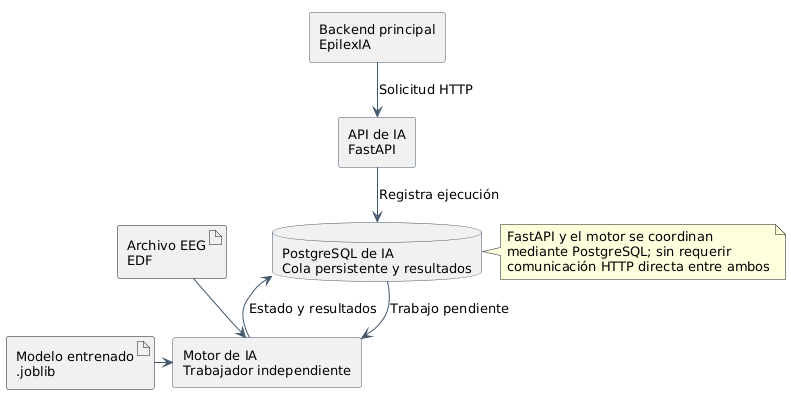
\includegraphics[width=\textwidth]{ThesisFigs/organizacion_procesamiento_ia_pgqueue.png}
    \caption{Organización del procesamiento de inteligencia artificial mediante cola persistente en EpilexIA.}
    \label{fig:organizacion-procesamiento-ia-pgqueue}
\end{figure}


\subsection{Preparación y procesamiento de señales EEG}
\label{subsec:preparacion-procesamiento-eeg-ia}

El procesamiento de señales electroencefalográficas mediante inteligencia artificial en EpilexIA parte de archivos digitales en formato EDF. El motor de inferencia accede al archivo asociado con la ejecución solicitada mediante una referencia a su ubicación en el almacenamiento, sin necesidad de transferir la totalidad de las muestras a través de la API de inteligencia artificial. Para interpretar el registro, el procedimiento utiliza la biblioteca MNE de Python.

El procedimiento de análisis forma parte del modelo de detección provisto por el equipo de ciencia de datos del proyecto, por lo que su diseño interno no integra el alcance del presente trabajo.
Para integrarlo, el motor considera sus etapas generales: la adaptación de las señales a un montaje bipolar longitudinal de 18 derivaciones, el remuestreo a 256~Hz, el filtrado, la segmentación en ventanas consecutivas de 10 segundos, la extracción de características de cada ventana y su normalización para cada registro.
La configuración de estas etapas se distribuye junto con el modelo entrenado, de modo que el motor aplica a cada estudio el mismo procedimiento con el que el modelo fue entrenado (Sección~\ref{subsec:modelo-vigente-hgb}).

El procesamiento se ejecuta de forma independiente de la navegación del especialista por la interfaz web. El trabajador obtiene las ejecuciones pendientes desde PostgreSQL, inicia el procedimiento de inferencia y actualiza la información de estado y resultados. Los intervalos temporales analizados se expresan en segundos relativos al inicio del registro, lo que permite relacionar las predicciones con las posiciones correspondientes dentro del estudio EEG.

Es importante distinguir este procedimiento del procesamiento realizado por el \textit{backend} principal para la visualización de señales. Mientras este último prepara segmentos destinados a la recuperación y navegación temporal del registro, el motor de inteligencia artificial construye características de las ventanas y aplica el modelo predictivo para identificar intervalos que podrían requerir revisión clínica.


\subsection{Generación e interpretación de resultados}
\label{subsec:generacion-interpretacion-resultados-ia}

Para cada ventana analizada, el modelo entrega una probabilidad de crisis.
Estos valores constituyen salidas del modelo y no deben interpretarse, por sí solos, como una confirmación clínica de actividad epiléptica.

La decisión de señalar un intervalo combina dos parámetros: un umbral de probabilidad y una cantidad mínima de ventanas consecutivas que deben superarlo.
Ambos se definen en el paquete del modelo.
Al registrarse una ejecución, el umbral aplicable se incorpora a sus datos, de manera que el valor utilizado permanece asociado al procesamiento correspondiente aunque la configuración se modifique posteriormente.
Los valores del modelo vigente se indican en la Sección~\ref{subsec:modelo-vigente-hgb}.

Durante el análisis, el motor genera un archivo temporal con la información de las ventanas procesadas y registra en PostgreSQL únicamente las que integran un intervalo señalado.

Cada resultado conservado se vincula con su ejecución de origen e incluye el tiempo de inicio y fin del intervalo, expresados en segundos respecto del comienzo del registro, así como la probabilidad de crisis utilizada para su selección. La relación con la ejecución permite recuperar el estudio asociado y la información necesaria para identificar el procesamiento que produjo el resultado. Las ventanas se registran individualmente, por lo que un intervalo señalado se presenta como una secuencia de registros consecutivos.

La finalización satisfactoria de una ejecución indica que el procedimiento concluyó conforme a su flujo operativo, pero no implica necesariamente la existencia de resultados positivos almacenados. Si ninguna ventana satisface los criterios de selección, el procesamiento puede finalizar con estado exitoso y sin registros de resultados. Asimismo, los estados de ejecución permiten diferenciar los trabajos pendientes o en curso de aquellos que finalizan, fallan, exceden el tiempo permitido o son cancelados.

En consecuencia, los intervalos generados por el subsistema de inteligencia artificial deben entenderse como indicaciones de posibles hallazgos que orientan la revisión del registro EEG. Su interpretación requiere considerar las señales originales y el contexto clínico del estudio. La decisión sobre la relevancia de cada intervalo corresponde al especialista, por lo que el componente automatizado cumple una función de apoyo y no sustituye la evaluación médica.


\subsection{Integración de resultados en la revisión clínica}
\label{subsec:integracion-resultados-revision-clinica}

La integración de los resultados de inteligencia artificial en EpilexIA tiene como propósito facilitar que el especialista examine los intervalos identificados durante el procesamiento automatizado en el contexto del estudio electroencefalográfico. Para ello, el sistema relaciona cada ejecución con el estudio clínico correspondiente y permite recuperar los resultados mediante los servicios de integración entre el \textit{backend} principal y la API de inteligencia artificial.

Una vez concluida la ejecución, el \textit{backend} principal puede consultar las ventanas que cumplen los criterios de detección y obtener sus límites temporales. Estos intervalos se expresan en segundos respecto del inicio del registro EEG, lo que permite relacionarlos con la posición correspondiente en las señales visualizadas. De este modo, los resultados automatizados funcionan como referencias temporales para orientar la inspección del registro, sin sustituir la observación directa de las señales.

La revisión clínica conserva una separación entre los resultados producidos por el modelo y las decisiones del especialista. La identificación automática de un intervalo no implica que este haya sido confirmado como un evento epiléptico. Su relevancia debe determinarse mediante el análisis de la actividad electroencefalográfica y de la información clínica disponible para el estudio.

El diseño contempla mecanismos para incorporar a los informes médicos las ventanas de inteligencia artificial seleccionadas durante la revisión. La asociación conserva la referencia a la ejecución y al resultado de origen, así como información descriptiva y de clasificación aportada por el profesional. Esta vinculación permite distinguir los intervalos identificados automáticamente de aquellos que el especialista decide utilizar como parte de su informe.

Asimismo, EpilexIA permite registrar anomalías y anotaciones definidas manualmente por el especialista, incluso cuando no corresponden a una ventana previamente detectada por el modelo. Las anotaciones manuales y las ventanas de inteligencia artificial incluidas en un informe se gestionan como conjuntos diferenciados y pueden sincronizarse con el subsistema de IA mediante interfaces específicas. Por consiguiente, la ausencia de una detección automática no impide que el profesional documente un hallazgo observado durante la revisión.

La información de retroalimentación clínica se conserva en estructuras específicas del subsistema de inteligencia artificial. En particular, las inclusiones de ventanas en informes permiten mantener su asociación con la revisión profesional, mientras que las anotaciones manuales registran observaciones originadas en la evaluación del especialista. Estos datos podrían servir como insumos para procesos posteriores de mejora de los modelos, pero su almacenamiento no implica que EpilexIA ejecute automáticamente un reentrenamiento.

La organización de los informes mantiene la responsabilidad de cada especialista sobre el contenido clínico que elabora. Así, la consulta de resultados automatizados y la selección de ventanas para un informe se integran al flujo de trabajo médico sin convertir las predicciones en conclusiones diagnósticas obligatorias. La interpretación final y la elaboración del informe corresponden al profesional responsable.

En síntesis, la integración de resultados vincula las ejecuciones de inteligencia artificial con la navegación temporal del EEG, la documentación de hallazgos y la elaboración de informes clínicos. El componente automatizado aporta referencias para la revisión, mientras que la valoración de su significado clínico permanece bajo el criterio del especialista.


\section{Diseño de seguridad y control de acceso}
\label{sec:seguridad-control-acceso}

El diseño de seguridad de EpilexIA contempla mecanismos destinados a controlar el acceso a las funcionalidades del sistema y a la información asociada con los pacientes, los estudios electroencefalográficos y los informes clínicos. Dada la naturaleza de estos datos, el acceso se organiza mediante la identificación de los usuarios, la asignación de permisos y la verificación de las condiciones necesarias para realizar cada operación.

La autenticación se realiza a través del \textit{backend} principal, que emite un \textit{token} de acceso para las sesiones válidas. Las solicitudes posteriores a los servicios protegidos incorporan dicho \textit{token}, cuya validez se comprueba antes de permitir el procesamiento de la operación. Este mecanismo se complementa con el registro de sesiones, lo que permite controlar la vigencia de los accesos autenticados.

La autorización combina permisos asociados a los roles del sistema con verificaciones adicionales sobre los recursos clínicos. Por ello, disponer de un permiso general para consultar o modificar estudios no implica necesariamente poder acceder a cualquier registro: determinadas operaciones también dependen de la relación del usuario con el estudio o el informe correspondiente.

En la aplicación web, las rutas y acciones disponibles se presentan de acuerdo con la autenticación y los permisos del usuario. Sin embargo, estas restricciones de interfaz no sustituyen las verificaciones realizadas por el \textit{backend}, que constituye el punto de control para autorizar las solicitudes recibidas.

Los siguientes apartados describen los mecanismos de autenticación, la organización de roles y permisos, las reglas de acceso a recursos clínicos y las consideraciones de protección de datos y comunicaciones contempladas en el diseño de EpilexIA.


\subsection{Autenticación de usuarios}
\label{subsec:autenticacion-usuarios}

La autenticación de usuarios en EpilexIA se realiza a través del \textit{backend} principal y constituye el mecanismo de identificación previo al acceso a los servicios protegidos. El proceso comienza cuando el usuario introduce sus credenciales en la interfaz web. Estas se remiten al servicio de autenticación, que comprueba su validez y las condiciones de acceso de la cuenta antes de establecer una sesión.

Cuando las credenciales son válidas, el \textit{backend} genera un \textit{token} de acceso en formato \textit{JSON Web Token} (JWT).
 El \textit{token} se firma digitalmente e incorpora información que permite identificar al usuario y determinar su período de vigencia. Asimismo, contiene un identificador único de \textit{token}, denominado \texttt{jti}, que se utiliza para relacionarlo con un registro de sesión persistido en la base de datos clínica. La respuesta de autenticación proporciona al \textit{frontend} la información necesaria para continuar las operaciones del usuario, incluidos sus permisos.

En las solicitudes posteriores, la aplicación web incorpora el \textit{token} mediante el encabezado HTTP \texttt{Authorization}, utilizando el esquema \texttt{Bearer}. Antes de permitir el acceso a los servicios protegidos, el \textit{backend} comprueba la firma y la expiración del JWT, extrae su identificador \texttt{jti} y verifica que exista una sesión vigente asociada. Si alguna de estas condiciones no se cumple, la solicitud no se considera autenticada.

La configuración de seguridad utiliza una política de procesamiento HTTP sin estado, denominada \texttt{stateless}. Esto significa que la autenticación no depende de una sesión HTTP tradicional mantenida entre solicitudes. No obstante, EpilexIA conserva registros de sesiones de usuario en la base de datos, lo que permite controlar la vigencia de los \textit{tokens} emitidos y revocarlos antes de que alcancen su fecha de expiración.

Una vez validado el \textit{token}, el \textit{backend} recupera la información actual del usuario y las autoridades correspondientes a sus permisos. De esta manera, la autenticación establece la identidad del solicitante, mientras que la autorización posterior determina qué operaciones puede realizar. La validación de un JWT, por sí sola, no concede acceso indiscriminado a los recursos clínicos del sistema.

El cierre de sesión dispone de una operación específica que identifica el \textit{token} utilizado y elimina el registro de sesión correspondiente. En consecuencia, aunque el JWT conserve una firma válida y no haya alcanzado su expiración, deja de ser aceptado cuando ya no existe una sesión vigente asociada a su identificador. Asimismo, el procedimiento de restablecimiento de contraseña contempla la invalidación de sesiones para impedir la continuidad de accesos previamente autorizados.

El diseño también contempla procedimientos de activación de cuentas y restablecimiento de contraseñas mediante \textit{tokens} específicos, distintos de los JWT utilizados para acceder a los servicios clínicos. Estos mecanismos permiten gestionar el establecimiento o la recuperación de credenciales sin confundir dichas operaciones con una sesión autenticada de uso ordinario.

En conjunto, la autenticación de EpilexIA combina la verificación de credenciales, la emisión de \textit{tokens} firmados y el control de sesiones persistidas. Esta organización proporciona una base para identificar a los usuarios y aplicar posteriormente las reglas de roles, permisos y acceso contextual a los recursos clínicos, desarrolladas en los siguientes apartados.


\subsection{Roles y permisos}
\label{subsec:roles-permisos}

El control de acceso de EpilexIA se organiza mediante un esquema de autorización basado en roles y permisos. Cada usuario dispone de un rol asociado con un conjunto de operaciones autorizadas, de acuerdo con las responsabilidades que desempeña dentro del sistema. Esta organización permite diferenciar las funciones administrativas, el registro y la preparación de estudios, y las actividades de revisión clínica.

El modelo vigente contempla tres roles: Administrador, Técnico y Especialista. El Administrador se orienta a la gestión de usuarios, roles y permisos, además de las operaciones de supervisión y administración disponibles en el sistema. El Técnico participa principalmente en el registro de pacientes y estudios electroencefalográficos, así como en la incorporación de los archivos correspondientes. El Especialista desarrolla las tareas clínicas de consulta y revisión de estudios, análisis de señales, registro de hallazgos y elaboración de informes médicos.

El Cuadro~\ref{tab:roles-permisos-epilexia} resume las responsabilidades principales de estos perfiles. Se trata de una descripción funcional de los roles, no de una enumeración exhaustiva de todas las autorizaciones almacenadas en la base de datos.

\begin{table}[H]
\centering
\caption{Responsabilidades principales de los roles de EpilexIA.}
\label{tab:roles-permisos-epilexia}
\small
\begin{tabular}{|p{0.20\textwidth}|p{0.68\textwidth}|}
\hline
\textbf{Rol} & \textbf{Responsabilidades principales} \\ \hline
Administrador & Gestión de usuarios, roles y permisos; acceso administrativo y supervisión de los recursos del sistema conforme a las autorizaciones disponibles. \\ \hline
Técnico & Registro y actualización de información de pacientes, creación de estudios EEG e incorporación de archivos asociados a los estudios en los que participa. \\ \hline
Especialista & Consulta y revisión de estudios EEG, análisis de señales, registro de anomalías y eventos, y creación y gestión de informes clínicos conforme a los permisos y reglas de acceso aplicables. \\ \hline
\end{tabular}
\end{table}

Los permisos se representan mediante identificadores asociados a recursos y acciones. Por ejemplo, \texttt{patients.list}, \texttt{studies.create}, \texttt{reports.update} y \texttt{anomalies.create} expresan autorizaciones para consultar pacientes, registrar estudios, actualizar informes y crear anomalías, respectivamente. Esta separación permite controlar operaciones concretas sin depender exclusivamente del nombre del rol.

La relación entre roles y permisos se mantiene en la base de datos clínica. Al autenticarse, el usuario recibe información sobre sus permisos, que la aplicación web utiliza para habilitar rutas y presentar las acciones correspondientes. En el \textit{backend}, los permisos se traducen en autoridades de seguridad y se verifican en los servicios protegidos antes de ejecutar las operaciones solicitadas.

La asignación de permisos puede administrarse mediante las funcionalidades destinadas a la gestión de roles. Por ello, el conjunto de acciones disponible para un usuario depende de las autorizaciones efectivamente asociadas a su rol, y no únicamente de la denominación de este. Las asignaciones iniciales previstas en los scripts de base de datos constituyen una configuración de referencia que puede diferir de la existente en una instalación administrada.

Es importante distinguir los permisos funcionales de las condiciones de acceso a un registro particular. Por ejemplo, disponer de autorización para consultar estudios no implica necesariamente poder visualizar cualquier estudio EEG. El sistema aplica comprobaciones adicionales según la participación del usuario y su relación con el recurso solicitado. Estas reglas de autorización contextual se desarrollan en el apartado siguiente.

De esta manera, la organización por roles y permisos proporciona un mecanismo para distribuir responsabilidades y restringir las operaciones disponibles, mientras que las verificaciones específicas sobre pacientes, estudios e informes complementan el control de acceso a la información clínica.


\subsection{Autorización sobre recursos clínicos}
\label{subsec:autorizacion-recursos-clinicos}

La autorización sobre recursos clínicos en EpilexIA complementa los permisos asociados a los roles mediante verificaciones relacionadas con el registro solicitado. Este mecanismo permite distinguir entre disponer de autorización para ejecutar una operación y estar habilitado para realizarla sobre un paciente, estudio electroencefalográfico o informe determinado. Las comprobaciones se efectúan en el \textit{backend} principal, de manera que la presentación de acciones en la interfaz web no constituye por sí sola una autorización suficiente.

En los servicios vinculados a estudios EEG, el control de acceso considera la relación del usuario con cada estudio. La consulta se permite al Administrador, al Técnico que registró el estudio, al Especialista responsable y a los especialistas incorporados como observadores, siempre que dispongan también de los permisos funcionales requeridos. Por el contrario, un Especialista que no mantiene una relación autorizada con el estudio no adquiere acceso únicamente por pertenecer al mismo rol clínico.

Las operaciones de modificación de los datos del estudio están sujetas a condiciones más restrictivas. De acuerdo con las reglas de acceso implementadas, estas operaciones se habilitan al Administrador o al Especialista responsable, según los permisos correspondientes. La condición de observador permite participar en la revisión del estudio, pero no otorga por sí misma autorización para modificar sus datos generales. Asimismo, el Técnico que registró el estudio no adquiere por ese hecho las facultades de modificación reservadas a otros participantes.

La incorporación de archivos asociados al estudio utiliza una comprobación específica. Además del permiso requerido para la operación, pueden realizar la carga el Administrador, el Especialista responsable y el Técnico creador del estudio. Esta capacidad se encuentra condicionada por el estado del registro: los estudios anulados no admiten nuevas cargas. De esta manera, la autorización considera tanto la relación del usuario con el estudio como las condiciones de la operación solicitada.

En el visualizador EEG, el acceso a señales, segmentos y otros recursos del estudio se apoya en las reglas de consulta previamente descritas. Por su parte, el registro y la modificación de anomalías y eventos EEG requieren permisos específicos y verificaciones adicionales sobre la participación del usuario. Esta separación evita equiparar la capacidad de observar las señales con la autorización para modificar los hallazgos asociados al estudio.

La gestión de informes médicos incorpora un control adicional basado en la autoría. EpilexIA permite que distintos especialistas vinculados a un mismo estudio elaboren informes propios. La relación entre el estudio, el informe y su autor se conserva en los registros correspondientes, y el sistema establece que cada especialista puede disponer de un único informe propio por estudio. Por tanto, tanto el Especialista responsable como los Especialistas incorporados como observadores autorizados pueden elaborar sus propios informes médicos asociados al estudio, siempre que dispongan de los permisos correspondientes. Cada informe pertenece al Especialista que lo creó y no puede ser modificado por otros profesionales.


La consulta de un informe perteneciente a otro profesional no implica autorización para modificarlo. Cuando un especialista accede a un informe ajeno mediante los servicios vinculados al estudio, la información se presenta en modo de solo lectura. La edición del informe propio requiere, además de los permisos funcionales, que se cumplan las condiciones relativas a su autoría y estado. La creación de nuevos informes también está condicionada por las reglas del proceso, entre ellas la inexistencia de un informe propio previo y las restricciones asociadas al cierre de informes del estudio.

En cuanto a los datos de pacientes, la autorización se organiza principalmente mediante permisos funcionales de consulta, creación y actualización. A diferencia de las comprobaciones contextuales aplicadas a los estudios, las operaciones generales sobre pacientes no se restringen al Técnico creador ni al Especialista asignado: dependen únicamente de los permisos del usuario. Esta distinción es relevante para describir con precisión el alcance de las verificaciones presentes en cada servicio.

Finalmente, las reglas de acceso contextual se aplican en los servicios que incorporan expresamente dichas comprobaciones. Algunas operaciones generales de búsqueda y exportación utilizan controles basados en permisos sin reproducir necesariamente todas las restricciones de participación de los servicios asociados a un estudio particular. Por ello, el diseño de seguridad debe analizarse considerando conjuntamente las autoridades exigidas por cada interfaz y las verificaciones adicionales realizadas por su lógica de aplicación.

En síntesis, la autorización sobre recursos clínicos combina permisos funcionales, relaciones de participación y condiciones propias de los registros. Esta organización permite diferenciar la consulta de estudios, la modificación de datos, la incorporación de archivos y la gestión de informes, manteniendo la responsabilidad de las decisiones clínicas en los especialistas habilitados.


\subsection{Protección de datos y comunicaciones}
\label{subsec:proteccion-datos-comunicaciones}

La protección de la información en EpilexIA comprende tanto los datos clínicos almacenados como las comunicaciones entre los componentes de la plataforma. Debido a que el sistema gestiona información de pacientes, registros electroencefalográficos, archivos de video e informes médicos, su diseño combina controles de acceso de aplicación con mecanismos de separación de servicios y medidas que deben completarse en el entorno de despliegue.

En el tratamiento de las credenciales, el sistema distingue las contraseñas utilizadas para autenticar a los usuarios de los \textit{tokens} de acceso emitidos para las sesiones. La creación y recuperación de cuentas se realizan mediante procedimientos específicos de activación y restablecimiento de contraseña. Por su parte, las solicitudes autenticadas utilizan \textit{tokens} JWT, cuya validación y revocación se describieron en el apartado~\ref{subsec:autenticacion-usuarios}. Estos mecanismos evitan que la autorización de las operaciones clínicas dependa únicamente de los controles visibles en la interfaz web.

La comunicación habitual comienza en el navegador y pasa por el servidor web Nginx, que entrega la aplicación y encamina las solicitudes hacia el \textit{backend} principal. Este último centraliza la autenticación, la autorización y el acceso a los recursos clínicos. La comunicación con el subsistema de inteligencia artificial se realiza mediante una interfaz de servicio diferenciada, que utiliza autenticación HTTP Basic con credenciales configuradas para la integración. En consecuencia, las credenciales del usuario clínico y las empleadas entre servicios cumplen funciones distintas.

El cifrado de las comunicaciones constituye una consideración específica del despliegue. El uso de HTTPS con TLS permite proteger la información transmitida entre el navegador y el punto de entrada del sistema frente a su lectura o alteración durante el transporte. En el entorno de despliegue utilizado, el acceso de los usuarios se realiza mediante HTTPS (Sección~\ref{subsec:despliegue-nube}), mientras que los servicios internos se comunican dentro de la red del propio entorno. La habilitación de HTTPS y la configuración de los certificados forman parte de la instalación en cada infraestructura donde se despliegue EpilexIA.

Los datos estructurados se conservan en bases PostgreSQL diferenciadas: una destinada a los registros clínicos y otra a las ejecuciones y resultados del subsistema de inteligencia artificial. Los archivos EEG y de video se mantienen en almacenamiento persistente separado de las tablas relacionales. De igual manera, los artefactos de los modelos de aprendizaje automático se alojan en recursos de archivos accesibles para los componentes que ejecutan las inferencias. Esta distribución permite administrar por separado los registros, los archivos de gran tamaño y los modelos utilizados.

La persistencia de estos recursos requiere medidas operativas adicionales. El diseño de despliegue mediante contenedores y volúmenes permite conservar la información aunque se detengan o reinicien los servicios, pero no reemplaza la necesidad de realizar copias de seguridad. Los recursos críticos del sistema son el almacenamiento de EEG y video, la base clínica y la base de inteligencia artificial, cuya conservación y respaldo deben contemplarse en la administración de la infraestructura.

La configuración de los servicios también incluye información sensible, como las credenciales de conexión a las bases de datos, la clave utilizada para firmar JWT y las credenciales de integración con la API de inteligencia artificial. Estos valores deben gestionarse en el entorno de operación y no incorporarse al contenido público de la aplicación web ni a la documentación distribuida. La protección efectiva de tales parámetros depende asimismo de las restricciones de acceso al servidor y a su configuración.

En cuanto al seguimiento técnico, EpilexIA dispone de mecanismos de registro que permiten relacionar solicitudes y operaciones mediante identificadores de trazabilidad. Las contraseñas y los \textit{tokens} se enmascaran en los registros estructurados. No obstante, la disponibilidad de estos registros no sustituye la aplicación de controles de acceso a los propios archivos de auditoría ni las políticas de conservación de información clínica.

En síntesis, el diseño de protección de datos y comunicaciones combina autenticación, autorización, separación de componentes, almacenamiento persistente y trazabilidad de operaciones. Su efectividad requiere complementar los controles implementados en la aplicación con una configuración segura de red, cifrado de transporte, gestión de credenciales y procedimientos de respaldo adecuados al entorno institucional de operación.

\section{Diseño de auditoría y trazabilidad}
\label{sec:diseno-auditoria-trazabilidad}

El diseño de auditoría y trazabilidad de EpilexIA contempla mecanismos para registrar operaciones relevantes del sistema y facilitar el seguimiento de las actividades realizadas sobre sus recursos. Dado que la plataforma administra información de pacientes, estudios electroencefalográficos e informes clínicos, resulta necesario disponer de registros que permitan reconocer las acciones efectuadas y el contexto en el que se produjeron.

La auditoría funcional se apoya en eventos persistidos en la base de datos clínica. Estos registros permiten identificar operaciones de negocio seleccionadas y conservar información sobre el actor, la acción realizada y los datos de contexto correspondientes. Su consulta proporciona una visión histórica de las actividades registradas, sin que ello implique que todas las solicitudes HTTP o todos los cambios internos generen necesariamente un evento de auditoría persistente.

Para facilitar la revisión de esta información, EpilexIA incorpora una vista de actividad reciente en el panel principal y una interfaz de consulta de auditorías. Esta última permite explorar los registros mediante paginación, ordenamiento cronológico y filtros combinables, de acuerdo con las autorizaciones exigidas por los servicios del \textit{backend}.

De manera complementaria, los componentes de aplicación producen registros técnicos que permiten seguir solicitudes y diagnosticar incidencias. Estos registros utilizan identificadores de trazabilidad para relacionar las etapas de una operación. En el subsistema de inteligencia artificial, el identificador de ejecución permite además vincular el seguimiento técnico con los estados y resultados del procesamiento asíncrono.

Por tanto, el diseño distingue entre los eventos de auditoría conservados para la consulta funcional y los registros técnicos utilizados para el seguimiento operativo. Los siguientes apartados describen el registro de operaciones y eventos, los mecanismos de consulta de auditorías y la trazabilidad de procesos e integraciones entre componentes.


\subsection{Registro de operaciones y eventos}
\label{subsec:registro-operaciones-eventos}

El registro de operaciones y eventos en EpilexIA tiene como finalidad conservar información sobre determinadas actividades realizadas dentro del sistema, permitiendo identificar las acciones ejecutadas y el contexto en el que se produjeron. Este mecanismo constituye una parte de la auditoría funcional y proporciona información para la revisión posterior de las operaciones relacionadas con los recursos administrados por la plataforma.

La implementación de auditoría se encuentra integrada en el \textit{backend}
principal. Para identificar las operaciones de negocio que generan
eventos de auditoría persistentes, el sistema utiliza la enumeración
\texttt{AuditEventType}. Estos eventos son publicados por los servicios
de aplicación y procesados mediante componentes específicos que
permiten conservarlos en la base de datos clínica.

De manera complementaria, el \textit{backend} utiliza la enumeración
\texttt{LogAction} para identificar operaciones registradas mediante
el mecanismo de \textit{logging} estructurado. Este mecanismo proporciona
trazas técnicas para el seguimiento de solicitudes y operaciones,
pero no implica necesariamente la generación de un evento de
auditoría persistente.

El registro de auditoría contempla operaciones relacionadas con la administración del sistema y la gestión de sus recursos. Entre ellas se encuentran determinadas acciones sobre usuarios, pacientes, estudios electroencefalográficos e informes médicos. La generación de estos registros depende de los puntos de la aplicación en los que se encuentra incorporado el mecanismo de auditoría, por lo que no debe interpretarse como un registro automático y exhaustivo de todas las solicitudes recibidas por el \textit{backend}.

Para conservar la información de los eventos, EpilexIA utiliza estructuras persistentes en la base de datos clínica PostgreSQL. Los registros de auditoría permiten asociar una operación con información contextual, como el usuario que la realizó, la acción registrada y el momento en que ocurrió. Según el tipo de evento, también pueden incorporarse referencias a los recursos involucrados y otros datos necesarios para describir la actividad.

La implementación incorpora componentes específicos para intervenir en el registro de eventos, entre ellos \texttt{AuditEventRecordListener}. Este componente forma parte del mecanismo utilizado por el \textit{backend} para gestionar la información de auditoría. Su participación debe distinguirse de los registros técnicos generales, ya que estos últimos están destinados principalmente al diagnóstico y seguimiento operativo de los servicios.

La conservación de eventos en la base de datos permite consultar posteriormente las actividades registradas sin depender exclusivamente de los mensajes producidos durante la ejecución de la aplicación. Esta persistencia facilita la construcción de vistas de actividad y servicios de consulta que recuperan los registros conforme a los criterios solicitados.

Es importante señalar que la existencia de un registro de auditoría no implica necesariamente que se conserve una copia completa del contenido anterior y posterior de cada recurso modificado. El alcance de la información disponible depende de los datos registrados para cada operación. Por esta razón, los eventos deben interpretarse como evidencias de actividades específicas y no como un mecanismo general de reconstrucción de todos los estados históricos del sistema.

Asimismo, el registro de una operación no sustituye las verificaciones de autenticación y autorización. Los controles de acceso determinan si una solicitud puede ejecutarse, mientras que la auditoría permite conservar información sobre las actividades para las cuales se ha previsto su registro. Ambos mecanismos cumplen funciones complementarias dentro del diseño de seguridad de EpilexIA.

En conjunto, el registro de operaciones y eventos proporciona una base persistente para el seguimiento de las actividades relevantes del sistema. Su integración con los servicios de consulta permite que los usuarios autorizados examinen posteriormente los eventos almacenados, identifiquen las operaciones registradas y dispongan de información contextual para su revisión.


\subsection{Consulta y seguimiento de auditorías}
\label{subsec:consulta-seguimiento-auditorias}

La consulta de auditorías en EpilexIA permite recuperar y examinar las operaciones registradas por el sistema, proporcionando información sobre las actividades realizadas y su contexto. Esta funcionalidad complementa el mecanismo de registro de eventos descrito anteriormente y facilita la revisión de las acciones ejecutadas sobre los recursos de la plataforma.

El sistema dispone de una vista de actividad reciente integrada en el panel principal, destinada a presentar un resumen de las operaciones registradas. Esta visualización permite identificar acontecimientos recientes sin necesidad de acceder inicialmente a la consulta completa de auditorías.


La Figura~\ref{fig:actividad-reciente} ilustra esta funcionalidad mediante una lista de operaciones registradas, acompañadas de sus respectivas fechas y horas. Asimismo, se observa el acceso a la consulta completa de auditorías.

\begin{figure}[H]
    \centering
    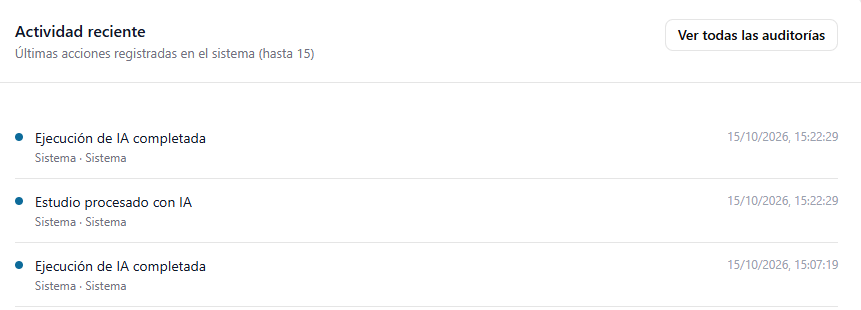
\includegraphics[width=0.90\textwidth]{ThesisFigs/actividad_reciente_epilexia.png}
    \caption{Vista de actividad reciente en el panel principal de EpilexIA.}
    \label{fig:actividad-reciente}
\end{figure}


Para una revisión más detallada, EpilexIA incorpora la interfaz denominada ``Ver todas las auditorías'', que permite consultar los registros mediante una tabla organizada. Esta interfaz presenta información de las operaciones registradas, incluyendo datos relacionados con el usuario, su rol, la acción realizada y la fecha del evento, según los atributos disponibles en cada registro.

La consulta contempla mecanismos de filtrado que permiten restringir los resultados conforme a diferentes criterios. Entre ellos se encuentran la búsqueda por usuario, la selección de roles y acciones, y la delimitación de fechas. La combinación de estos filtros facilita la localización de actividades específicas dentro del conjunto de registros disponibles.


En particular, el filtrado por fecha utiliza un control de selección que permite indicar el día de interés, mientras que la selección de roles se realiza mediante las opciones disponibles en el sistema. Estos controles reducen la necesidad de introducir manualmente determinados valores y contribuyen a mantener criterios de búsqueda consistentes.

Los resultados se presentan mediante paginación, de manera que la interfaz recupera y muestra una cantidad limitada de registros por página. Este mecanismo evita presentar simultáneamente la totalidad de los eventos almacenados y facilita la navegación entre los resultados de una consulta. Asimismo, el ordenamiento permite organizar los registros conforme a los criterios admitidos por el servicio, incluyendo su secuencia temporal.


La Figura~\ref{fig:consulta-auditorias} presenta
la interfaz de consulta de auditorías de EpilexIA.
En ella se observan los registros de actividad
organizados por fecha y hora, evento, actor,
rol y contexto, junto con los controles de
filtrado y paginación disponibles.


\begin{figure}[H]
    \centering
    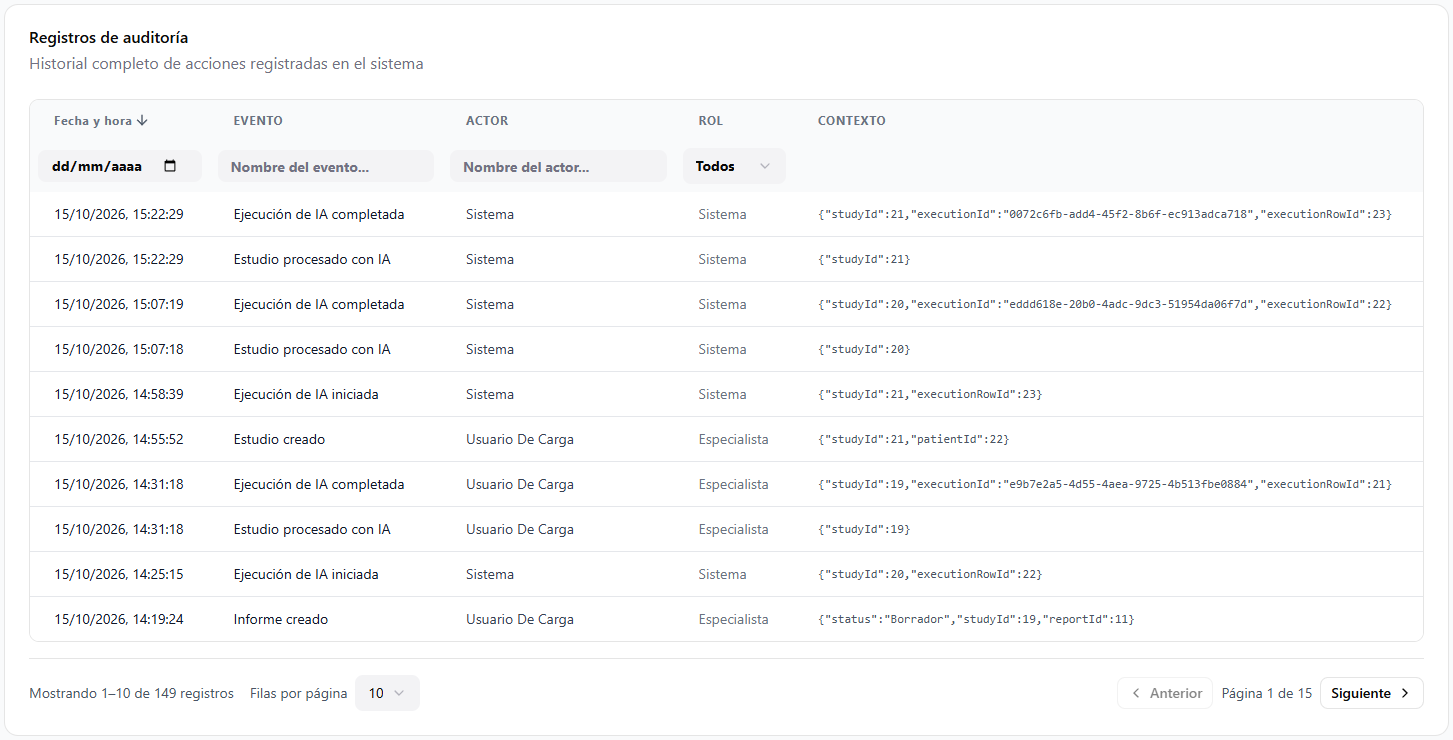
\includegraphics[width=\textwidth]{ThesisFigs/consulta_auditorias_epilexia.png}
    \caption{Consulta, filtrado y paginación de auditorías en EpilexIA.}
    \label{fig:consulta-auditorias}
\end{figure}


La recuperación de la información se realiza mediante servicios REST del \textit{backend} principal. Estos servicios reciben los parámetros de búsqueda y paginación, consultan los registros disponibles y devuelven los resultados correspondientes a la aplicación web. El procesamiento de los criterios de consulta en el servidor permite mantener una separación entre la presentación de los datos y la lógica encargada de recuperarlos.

El acceso a las funcionalidades de auditoría se encuentra sujeto a los permisos definidos para los usuarios del sistema. La interfaz web presenta las opciones correspondientes a las autorizaciones disponibles, mientras que el \textit{backend} verifica los permisos requeridos antes de responder a las solicitudes de consulta.

Es importante señalar que la información presentada corresponde a los eventos efectivamente registrados por los mecanismos de auditoría de EpilexIA. Por consiguiente, la ausencia de una actividad en los resultados de búsqueda no demuestra, por sí sola, que ninguna operación relacionada haya ocurrido, dado que el alcance del registro depende de los eventos contemplados por la aplicación.

En conjunto, la consulta y el seguimiento de auditorías proporcionan herramientas para examinar las actividades registradas, localizar operaciones mediante filtros y navegar por los resultados de manera organizada. Estas funcionalidades contribuyen a la supervisión administrativa y complementan los mecanismos de seguridad y trazabilidad del sistema.

% FIGURA OPCIONAL: activar después de subir la imagen a ThesisFigs.
% La Figura~\ref{fig:consulta-auditorias-epilexia} presenta la interfaz de consulta de auditorías.
% \begin{figure}[H]
%     \centering
%     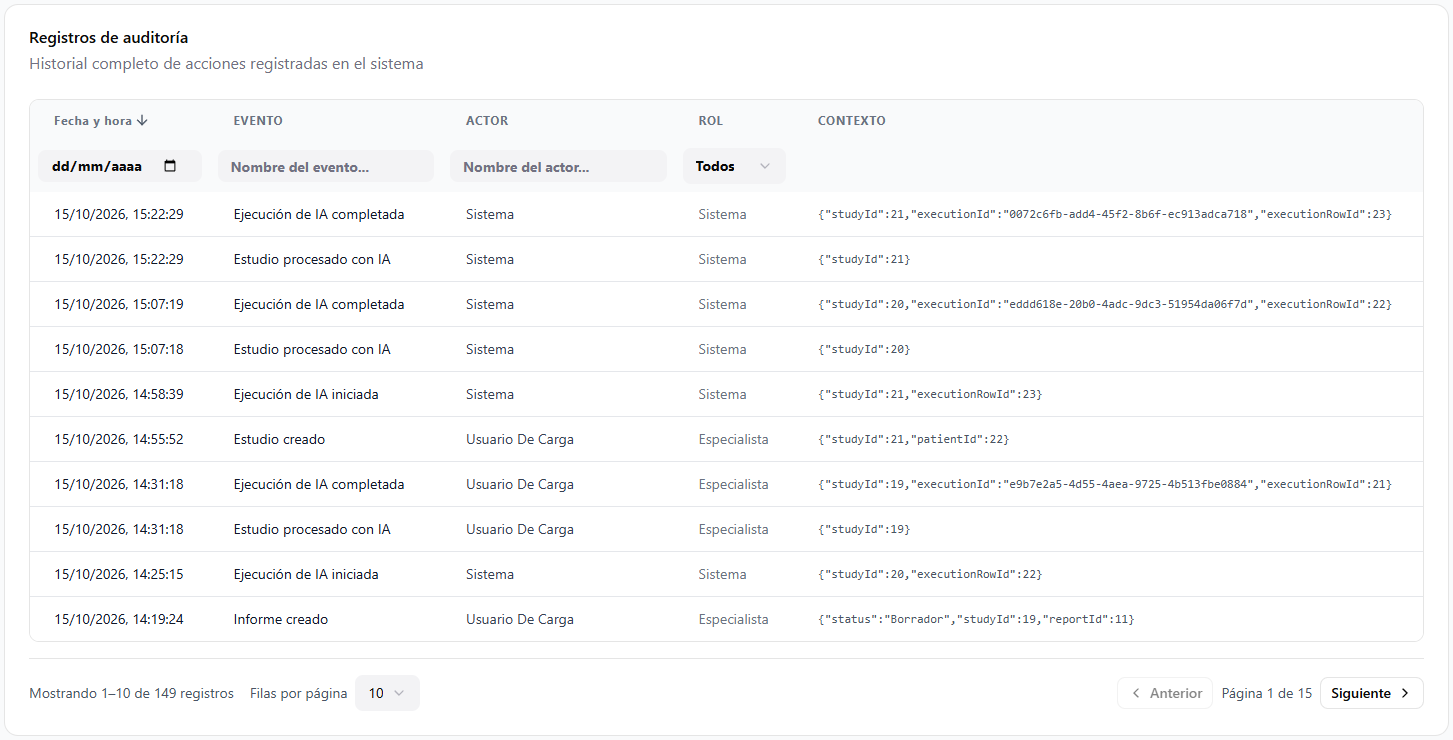
\includegraphics[width=\textwidth]{ThesisFigs/consulta_auditorias_epilexia.png}
%     \caption{Interfaz de consulta y filtrado de auditorías del sistema EpilexIA.}
%     \label{fig:consulta-auditorias-epilexia}
% \end{figure}


\subsection{Trazabilidad de procesos e integración}
\label{subsec:trazabilidad-procesos-integracion}

La trazabilidad de procesos en EpilexIA comprende los mecanismos
que permiten relacionar las solicitudes recibidas por los
servicios de aplicación con las operaciones ejecutadas por
sus distintos componentes. Esta capacidad resulta especialmente
relevante en los procedimientos que involucran varias etapas
de procesamiento o requieren comunicación entre servicios
independientes.

En el \textit{backend} principal, los registros técnicos permiten
conservar información sobre el procesamiento de solicitudes
y las incidencias que pueden producirse durante su ejecución.
Para facilitar su seguimiento, se utilizan identificadores
de trazabilidad que permiten relacionar los mensajes
correspondientes a una misma operación. Estos registros
cumplen una función operativa y deben distinguirse de los
eventos de auditoría funcional almacenados en la base de
datos clínica.

La integración con el subsistema de inteligencia artificial
incorpora un mecanismo adicional de identificación. Cada
solicitud de procesamiento aceptada se asocia con un
identificador de ejecución, denominado
\texttt{executionId}, que permite reconocer el trabajo
correspondiente durante las distintas etapas de su ciclo
de vida. Este identificador constituye una referencia
para consultar el estado del procesamiento y recuperar
los resultados generados.

La API de inteligencia artificial registra la ejecución
en su base de datos PostgreSQL. Posteriormente, el motor
independiente obtiene los trabajos pendientes, realiza
el procesamiento de las señales EEG y actualiza la
información correspondiente a sus estados y resultados.
La persistencia de estos registros permite seguir
el avance del trabajo sin depender de una conexión
HTTP continua entre la API y el motor. La organización
de estos componentes y su mecanismo de coordinación
mediante PostgreSQL se ilustran en la
Figura~\ref{fig:organizacion-procesamiento-ia-pgqueue}.


El seguimiento de las ejecuciones contempla estados
que permiten diferenciar los trabajos pendientes,
aquellos que se encuentran en procesamiento y los
que han finalizado. Asimismo, se consideran situaciones
de fallo, cancelación o superación del tiempo permitido.
Esta información permite distinguir entre la aceptación
inicial de una solicitud y la finalización efectiva
del análisis automatizado.

La relación entre los componentes también se apoya
en los identificadores de los estudios clínicos.
El \textit{backend} principal conserva la información del
estudio EEG, mientras que el subsistema de inteligencia
artificial registra las ejecuciones y los resultados
asociados mediante referencias lógicas. Dado que
ambos subsistemas utilizan bases de datos independientes,
estas referencias permiten establecer la correspondencia
entre sus registros sin requerir claves foráneas
entre las dos bases de datos.

Los resultados del procesamiento mantienen su
asociación con la ejecución que los produjo. De esta
manera, es posible identificar el análisis de origen
de los intervalos detectados y relacionarlos con el
estudio electroencefalográfico correspondiente. Esta
vinculación facilita la recuperación de información
desde los servicios de integración y su presentación
durante la revisión clínica.

De forma complementaria, los eventos de auditoría
funcional permiten conservar determinadas acciones
relacionadas con el inicio y la finalización de
procesamientos de inteligencia artificial, cuando
estas operaciones se encuentran contempladas por
los mecanismos de registro del \textit{backend}. Su finalidad
es documentar actividades relevantes para la consulta
posterior, mientras que los estados de ejecución y
los registros técnicos proporcionan información
más específica para el seguimiento operativo.

Es importante señalar que estos mecanismos no
constituyen necesariamente una traza única y completa
de todas las operaciones realizadas por los componentes.
El nivel de detalle disponible depende de los
identificadores propagados, los registros generados
por cada servicio y los eventos efectivamente
persistidos durante el procesamiento.

En conjunto, la trazabilidad de procesos e integración
de EpilexIA combina identificadores de solicitudes,
referencias a estudios clínicos, identificadores de
ejecución y registros de estado. Esta organización
facilita el seguimiento de los procedimientos
distribuidos, la identificación de incidencias y
la relación entre las operaciones técnicas y los
recursos clínicos involucrados.


\section{Diseño de interfaz de usuario}
\label{sec:diseno-interfaz-usuario}

El diseño de la interfaz de usuario de EpilexIA se orienta a facilitar la interacción de los distintos perfiles con las funcionalidades del sistema. Para ello, considera las necesidades de administración, de registro y gestión de estudios electroencefalográficos, de identificación de pacientes durante la creación de estudios y de revisión clínica.

La organización de la interfaz contempla los tres
roles definidos en el sistema: Administrador, Técnico
y Especialista. Cada perfil dispone de opciones de
navegación y acciones relacionadas con sus permisos,
de manera que las funcionalidades presentadas
correspondan a las tareas que puede desempeñar.
Esta diferenciación contribuye a organizar el acceso
a los recursos y a reducir la exposición de opciones
que no forman parte de las responsabilidades del
usuario.

La aplicación web se desarrolla mediante React y
utiliza componentes reutilizables para estructurar
las pantallas, los formularios, las tablas de datos
y los controles de interacción. Su diseño contempla
la adaptación de los elementos visuales a diferentes
dimensiones de pantalla, procurando mantener una
distribución adecuada de la información y facilitar
la navegación entre las funcionalidades disponibles.

Una parte central del diseño corresponde a la
visualización de estudios EEG. Debido a la naturaleza
temporal de las señales electroencefalográficas,
esta interfaz incorpora mecanismos de navegación
por el registro, selección de montajes, ajuste de
filtros y sensibilidad, así como opciones para ampliar
el área de visualización. Estos controles permiten
al especialista examinar las señales y relacionarlas
con los eventos y hallazgos asociados al estudio.


El diseño también contempla la presentación de los resultados de inteligencia artificial disponibles para cada estudio. Los intervalos registrados se integran en el entorno de revisión clínica como información complementaria, permitiendo al Especialista consultar las señales correspondientes y determinar su relevancia. Asimismo, la interfaz facilita el registro de anomalías, eventos y la elaboración de informes médicos vinculados al estudio.


En las operaciones de administración y gestión,
la interfaz utiliza formularios, tablas y mecanismos
de búsqueda para facilitar la consulta y actualización
de la información. Estas funcionalidades se complementan
con mensajes de estado y controles de interacción
que permiten comunicar al usuario el resultado de
las operaciones realizadas.

Los siguientes apartados describen la organización
general de la interfaz, las pantallas destinadas
a la administración y gestión de estudios, el
visualizador EEG y los componentes utilizados
para la revisión clínica y elaboración de informes.


\subsection{Organización general de la interfaz}
\label{subsec:organizacion-general-interfaz}

La interfaz web de EpilexIA se organiza mediante
pantallas destinadas a las principales actividades
del sistema. Su estructura permite que los usuarios
accedan a las funcionalidades correspondientes a
su perfil y mantengan una navegación consistente
entre las operaciones de administración, gestión
de estudios y revisión clínica.

El acceso a la aplicación comienza con una pantalla
de autenticación, desde la cual el usuario introduce
sus credenciales. Una vez completado el proceso
de identificación, el sistema presenta el entorno
de trabajo correspondiente a los permisos asociados
a su cuenta. Esta organización permite diferenciar
las opciones disponibles sin requerir interfaces
completamente independientes para cada perfil.

El panel principal constituye el punto de entrada
a las funcionalidades del sistema. Su contenido
se organiza mediante elementos de resumen y accesos
a las operaciones habituales del usuario. De acuerdo
con el perfil autenticado, pueden presentarse
indicadores relacionados con pacientes, estudios
electroencefalográficos, informes médicos y
procesamientos mediante inteligencia artificial,
así como accesos a las secciones habilitadas.


La Figura~\ref{fig:panel-principal-especialista}
presenta la organización del panel principal de
EpilexIA correspondiente al perfil Especialista.
En ella se observan los indicadores de resumen,
los accesos rápidos a las funcionalidades
disponibles y la sección de actividad reciente.


\begin{figure}[H]
    \centering
    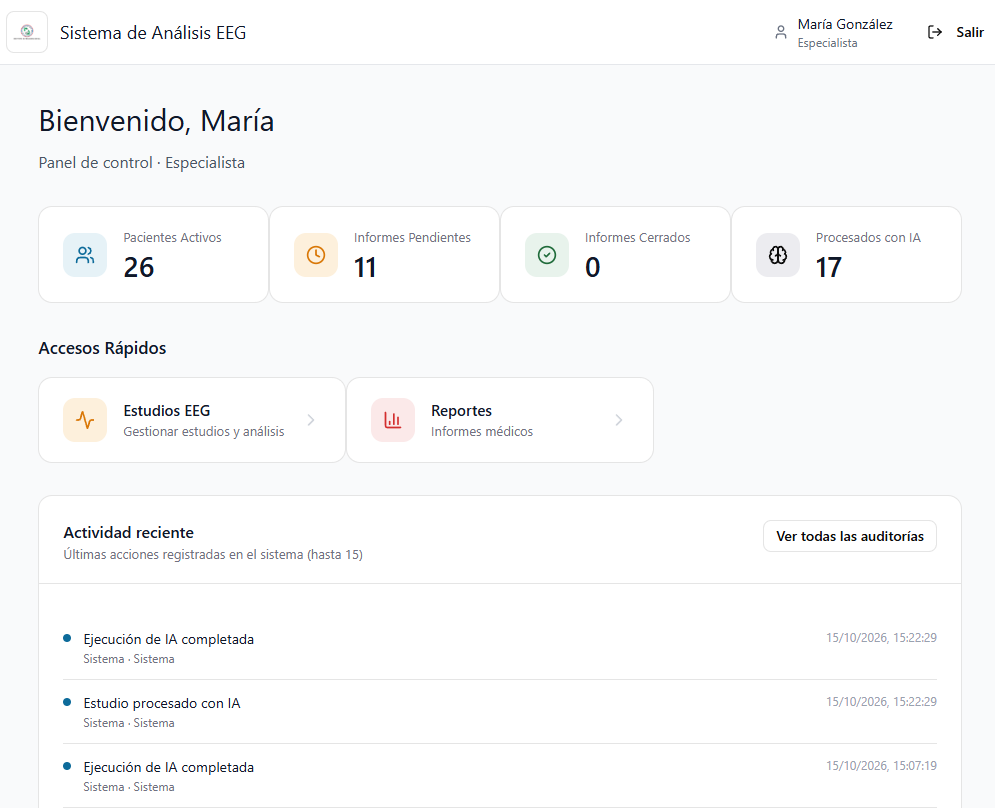
\includegraphics[width=\textwidth]{ThesisFigs/panel_principal_especialista.png}
    \caption{Organización del panel principal de EpilexIA
    correspondiente al perfil Especialista.}
    \label{fig:panel-principal-especialista}
\end{figure}


La navegación se estructura alrededor de las principales entidades y procesos administrados por EpilexIA. Las interfaces de estudios reúnen las operaciones relacionadas con su registro, seguimiento y acceso a los archivos asociados. Durante la creación de un estudio, el usuario puede seleccionar un paciente existente o registrar uno nuevo. Desde el entorno de un estudio, los usuarios autorizados pueden acceder a las funcionalidades de visualización de señales y revisión clínica.

La presentación de las acciones considera los
permisos del usuario autenticado. Por ejemplo,
las operaciones administrativas se orientan al
perfil Administrador, las actividades de registro
y preparación de estudios corresponden principalmente
al Técnico, y las herramientas de análisis e
informes clínicos se destinan al Especialista.
Esta diferenciación se refleja en los accesos,
controles y operaciones disponibles en cada pantalla.

Para mantener una experiencia de navegación
uniforme, la aplicación utiliza componentes
reutilizables en la presentación de información.
Entre ellos se encuentran tablas de registros,
formularios, controles de búsqueda, botones
de acción y elementos de navegación. La utilización
de estos componentes favorece la consistencia
visual y funcional entre las diferentes secciones
del sistema.

Las pantallas que presentan conjuntos de registros
incorporan mecanismos de búsqueda y organización
de resultados, según las características de cada
funcionalidad. Asimismo, los formularios permiten
introducir o actualizar información mediante
campos y controles específicos. Estas operaciones
se complementan con mecanismos de validación
y mensajes que comunican al usuario el estado
de las solicitudes realizadas.

La organización de la interfaz también considera
la adaptación a diferentes dimensiones de pantalla.
Para ello, la distribución de los elementos se
ajusta según el espacio disponible, procurando
conservar la accesibilidad de los controles y
la legibilidad de la información. No obstante,
las funcionalidades de análisis de señales EEG
requieren una superficie de visualización adecuada
debido a la cantidad de información gráfica
presentada simultáneamente.

En conjunto, esta organización proporciona
una estructura común para las distintas actividades
de EpilexIA y permite integrar la gestión
administrativa, el registro de estudios y la
revisión clínica dentro de una misma aplicación
web. Las características particulares de las
interfaces correspondientes a estos procesos
se desarrollan en los siguientes apartados.


\subsection{Interfaces de administración y gestión de estudios}

Las interfaces de administración y gestión de estudios de EpilexIA
permiten realizar las operaciones necesarias para organizar los
usuarios del sistema y administrar los estudios
electroencefalográficos. Estas pantallas utilizan formularios,
tablas de registros y controles de navegación que facilitan la
consulta y actualización de la información, de acuerdo con las
funcionalidades habilitadas para cada perfil.

En el ámbito administrativo, el sistema dispone de interfaces
orientadas a la gestión de usuarios y sus autorizaciones. Estas
permiten consultar la información de las cuentas, realizar
operaciones de administración y gestionar los roles y permisos
disponibles. La presentación de estas funcionalidades se organiza
mediante controles que facilitan la identificación de los registros
y la ejecución de las acciones correspondientes.

La administración de usuarios se encuentra diferenciada de las
actividades relacionadas con los estudios EEG. Mientras que el
perfil Administrador dispone de las funcionalidades de gestión de
cuentas y autorizaciones, los perfiles Técnico y Especialista
acceden principalmente a las operaciones de registro, consulta
y revisión de estudios, conforme a los permisos que tengan
asignados.

La gestión de estudios electroencefalográficos constituye una de
las funcionalidades centrales de la aplicación. La interfaz
correspondiente permite consultar los estudios registrados,
aplicar criterios de búsqueda y acceder a las operaciones
disponibles sobre cada uno de ellos. Los registros se presentan
mediante una tabla que incluye información del paciente, fechas
de creación y actualización, especialista responsable, estado
del estudio y procesamiento mediante inteligencia artificial.

La interfaz incorpora filtros que permiten localizar estudios
según diferentes criterios, entre ellos el nombre del paciente,
las fechas, el especialista responsable y el estado del estudio y del procesamiento mediante inteligencia artificial. Estos controles facilitan la identificación de
los registros y el seguimiento de las actividades relacionadas
con los estudios EEG.


La Figura~\ref{fig:gestion-estudios-eeg} presenta la interfaz
de gestión de estudios electroencefalográficos de EpilexIA,
en la que se observan los controles de búsqueda, los campos
de información y la opción de creación de nuevos estudios.


\begin{figure}[H]
    \centering
    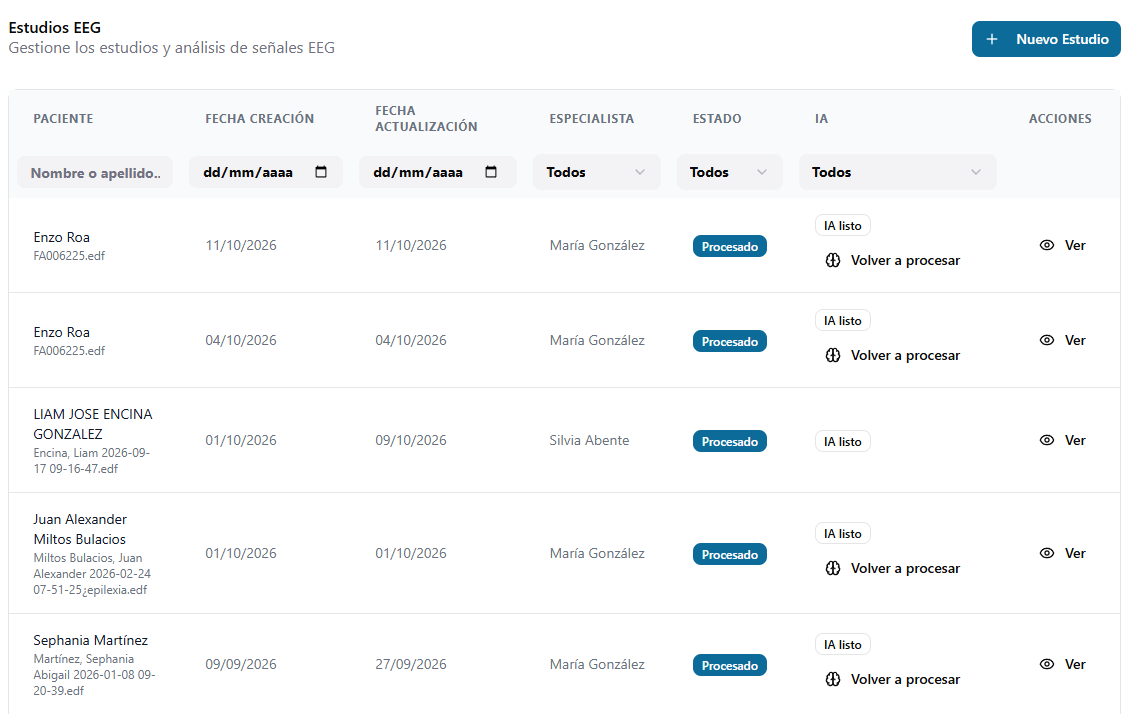
\includegraphics[width=\textwidth]{ThesisFigs/gestion_estudios_eeg.png}
    \caption{Interfaz de gestión de estudios EEG de EpilexIA.}
    \label{fig:gestion-estudios-eeg}
\end{figure}


El registro de un nuevo estudio se realiza mediante un formulario que permite seleccionar al paciente asociado e incorporar el archivo de señales EEG en formato EDF. La interfaz presenta diferencias según el perfil del usuario: en el caso del Técnico, se requiere seleccionar al especialista responsable del estudio, mientras que para el perfil Especialista dicho campo no se muestra. Asimismo, el formulario ofrece la posibilidad de adjuntar un video de monitoreo en formato MP4 o mediante archivos correspondientes a una grabación EZVideo.

Cuando el paciente requerido no se encuentra disponible en
el selector, la aplicación permite registrar uno nuevo sin
abandonar el proceso de creación del estudio. Esta operación
se realiza mediante un formulario que contempla datos de
identificación, información personal y datos de contacto.
De esta manera, el registro de pacientes se integra como
una funcionalidad complementaria a la creación de estudios
EEG, sin constituir un módulo independiente de gestión
de pacientes.

La Figura~\ref{fig:nuevo-estudio-eeg} presenta el formulario de creación de estudios EEG correspondiente al perfil Especialista. En ella se observan el campo de selección del paciente, así como los controles para incorporar el archivo EEG y, opcionalmente, un video de monitoreo.

\begin{figure}[H]
    \centering
    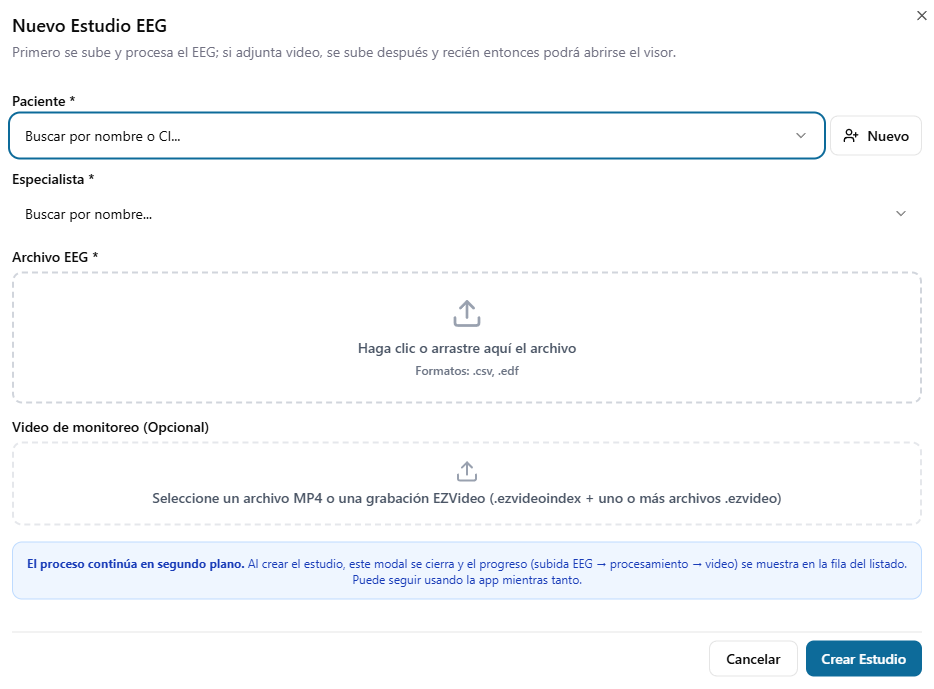
\includegraphics[width=\textwidth]{ThesisFigs/nuevo-estudio-eeg.png}
    \caption{Formulario de creación de estudios EEG correspondiente al perfil Especialista de EpilexIA.}
    \label{fig:nuevo-estudio-eeg}
\end{figure}

La creación del estudio contempla operaciones de carga y
procesamiento de archivos que continúan en segundo plano.
Una vez iniciado el procedimiento, el usuario puede seguir
utilizando la aplicación, mientras que el avance de las
operaciones se presenta en el listado de estudios. Este
mecanismo permite integrar la incorporación de archivos
y su preparación para la visualización posterior.

La organización de las pantallas de estudios también facilita
el acceso a las funcionalidades posteriores del proceso.
Desde un estudio registrado, los usuarios habilitados pueden
acceder a la visualización de señales electroencefalográficas
y a las herramientas de revisión clínica. De esta manera,
el registro inicial de los estudios se integra con las
actividades de análisis y elaboración de informes.

Las operaciones de consulta y actualización se complementan
con controles de búsqueda, acciones contextuales y mensajes
de estado. Estos elementos permiten localizar información,
identificar las operaciones disponibles y conocer el resultado
de las solicitudes realizadas, manteniendo una organización
consistente entre las distintas interfaces de gestión.

En conjunto, las interfaces de administración y gestión de
estudios proporcionan los medios necesarios para organizar
los usuarios del sistema, registrar estudios EEG e incorporar
los archivos utilizados durante la revisión clínica. Su
diseño establece una continuidad entre la administración
de cuentas, la preparación de estudios y el acceso a las
herramientas especializadas de análisis electroencefalográfico.


\subsection{Interfaz de visualización y análisis de señales EEG}

La interfaz de visualización y análisis de señales electroencefalográficas constituye uno de los componentes centrales de EpilexIA. Su diseño está orientado a facilitar la exploración de los registros EEG y proporcionar al especialista herramientas para examinar la actividad eléctrica cerebral, identificar posibles alteraciones y relacionar los hallazgos con la información asociada al estudio.

El acceso al visualizador se realiza desde la interfaz de gestión de estudios, mediante las acciones disponibles para cada registro. Una vez seleccionado un estudio, el sistema presenta las señales electroencefalográficas correspondientes, organizadas por canales y representadas gráficamente en función del tiempo. Esta disposición permite observar simultáneamente diferentes derivaciones y analizar su comportamiento durante el intervalo seleccionado.

La organización del visualizador contempla un área principal destinada a la representación de las señales EEG y un conjunto de controles que permiten modificar las condiciones de visualización. Estos elementos se distribuyen de manera que el usuario pueda realizar ajustes durante la exploración del registro sin abandonar el entorno de análisis.

La Figura~\ref{fig:interfaz-general-eeg} presenta la interfaz general de visualización y análisis de señales EEG de EpilexIA. En ella se observa la distribución del área de representación de las señales, los controles de configuración y navegación temporal, el panel de anomalías y el espacio destinado a la elaboración del informe médico.

\begin{figure}[H]
    \centering
    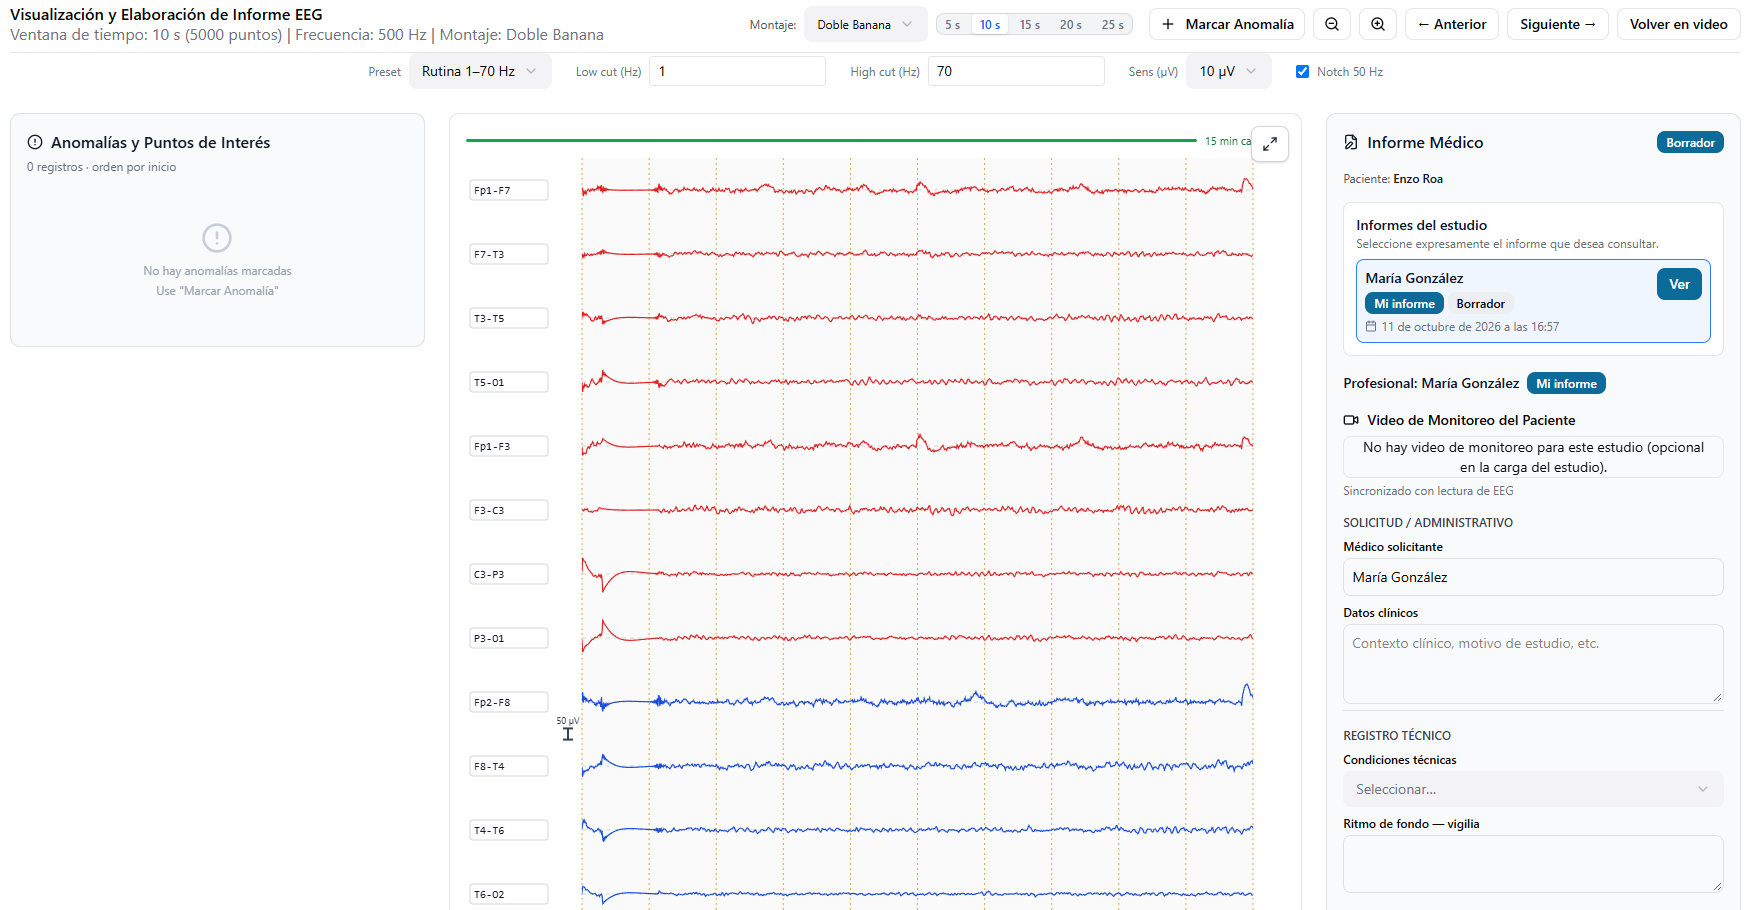
\includegraphics[width=\textwidth]{ThesisFigs/interfaz-general-eeg.png}
    \caption{Interfaz general de visualización y análisis de señales EEG de EpilexIA.}
    \label{fig:interfaz-general-eeg}
\end{figure}

Entre las funcionalidades disponibles se encuentra la navegación temporal, que permite desplazarse a lo largo del registro electroencefalográfico y examinar diferentes intervalos de tiempo. La interfaz incorpora controles para avanzar y retroceder por la señal, así como opciones para ajustar la ventana temporal representada. De esta manera, el especialista puede explorar tanto segmentos específicos como diferentes partes del estudio.

El visualizador también permite seleccionar montajes electroencefalográficos, mediante los cuales se determina la organización de las derivaciones presentadas. Esta funcionalidad facilita la revisión de las señales desde distintas configuraciones de canales, de acuerdo con las necesidades del análisis. Entre las configuraciones contempladas se encuentran los montajes bipolares y referenciales utilizados en la interpretación de registros EEG.

Otro elemento importante corresponde a los controles de filtrado y sensibilidad. Los filtros permiten ajustar la representación de las señales según los parámetros disponibles en la interfaz, mientras que el control de sensibilidad, expresado en microvoltios ($\mu$V), permite modificar la escala vertical de las ondas. Estos ajustes contribuyen a mejorar la observación de determinadas características de la actividad electroencefalográfica, sin modificar el archivo original del estudio.

Como herramienta complementaria, el visualizador incorpora un espectrograma que permite representar la distribución de la actividad de las señales EEG en función del tiempo y la frecuencia. Esta representación proporciona una perspectiva adicional para la exploración del registro electroencefalográfico.

Para ampliar el espacio destinado al análisis, EpilexIA incorpora un modo de pantalla completa. Esta funcionalidad permite visualizar las señales EEG en un área de mayor tamaño, reduciendo la presencia de otros elementos de la interfaz. El usuario puede continuar utilizando los controles de análisis disponibles y regresar posteriormente a la vista habitual.

La Figura~\ref{fig:visualizador-eeg-pantalla-completa} presenta el visualizador EEG en modo de pantalla completa, donde se observan simultáneamente múltiples canales electroencefalográficos, los controles laterales de navegación y el espectrograma ubicado en la parte inferior de la interfaz.

\begin{figure}[H]
    \centering
    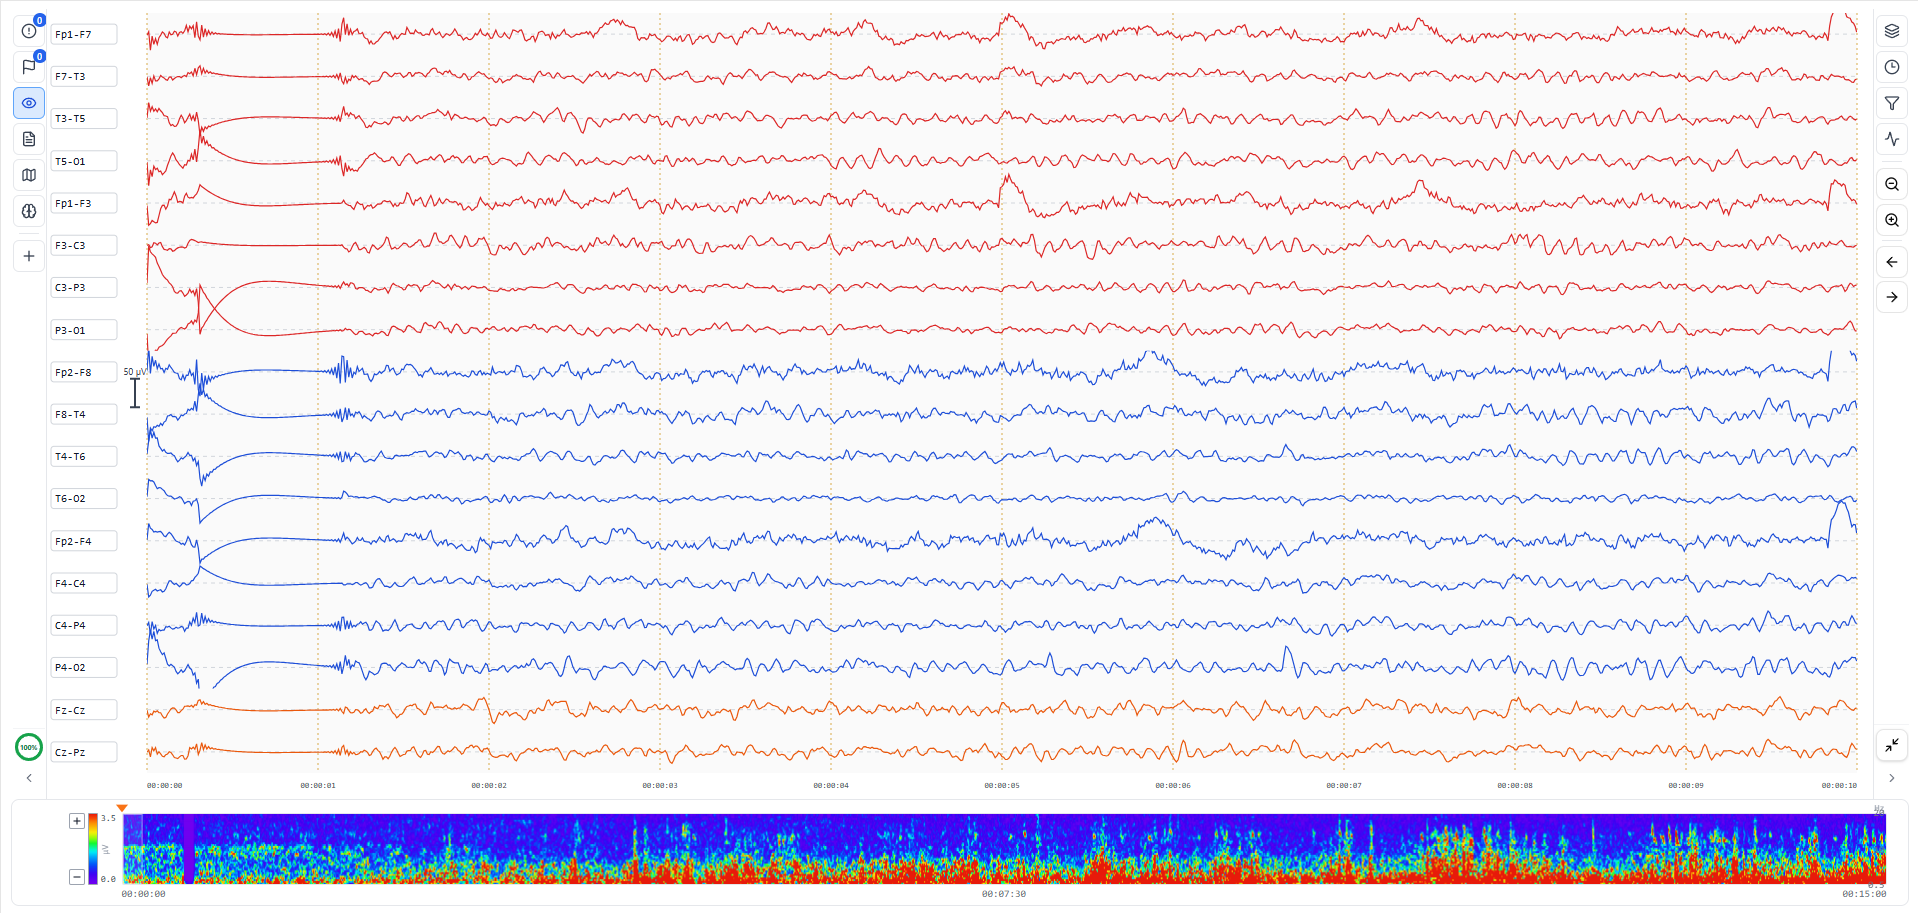
\includegraphics[width=\textwidth]{ThesisFigs/visualizador-eeg-pantalla-completa.png}
    \caption{Visualizador de señales EEG en modo de pantalla completa de EpilexIA.}
    \label{fig:visualizador-eeg-pantalla-completa}
\end{figure}

La interfaz también contempla la presentación de información relacionada con anomalías y eventos asociados al estudio. Estos elementos permiten vincular determinados intervalos del registro con observaciones realizadas durante su revisión. Asimismo, cuando existen resultados de procesamiento mediante inteligencia artificial, el especialista puede utilizarlos como información complementaria para orientar la exploración de segmentos de interés.

La visualización de las señales se integra con las demás funcionalidades de revisión clínica de EpilexIA. De esta manera, el especialista puede examinar los registros electroencefalográficos y relacionar los hallazgos observados con las actividades de documentación y elaboración de informes médicos correspondientes al estudio.

En conjunto, el diseño del visualizador EEG reúne herramientas de navegación, configuración y exploración de señales dentro de una misma interfaz. Su organización busca facilitar el análisis de registros electroencefalográficos y proporcionar un entorno de trabajo que apoye la revisión clínica realizada por el especialista.

\subsection[Interfaces de revisión clínica y elaboración de informes médicos]
{Interfaces de revisión clínica y elaboración de\\informes médicos}

Las interfaces de revisión clínica y elaboración de informes médicos de EpilexIA están orientadas a facilitar la documentación de los hallazgos identificados durante el análisis de los estudios electroencefalográficos. Estas funcionalidades permiten al especialista relacionar las observaciones realizadas sobre las señales EEG con la información clínica correspondiente y organizar los resultados de su evaluación dentro de un mismo entorno de trabajo.

La revisión clínica se desarrolla a partir de los estudios registrados en el sistema. Una vez que el especialista accede a un estudio, dispone de herramientas para examinar las señales electroencefalográficas, identificar segmentos de interés y registrar observaciones relacionadas con posibles alteraciones. Estas operaciones se integran con el visualizador EEG, permitiendo mantener una relación entre los hallazgos documentados y los intervalos temporales del registro.

Entre las funcionalidades disponibles se encuentra el registro de anomalías y eventos asociados al estudio. Estas herramientas permiten documentar situaciones identificadas durante la exploración de las señales y vincularlas con determinados segmentos del registro electroencefalográfico. La información registrada constituye un recurso de apoyo para la revisión posterior y la elaboración del informe médico.


Cuando un estudio dispone de resultados de inteligencia artificial previamente almacenados, la interfaz permite consultar los intervalos señalados en dichos registros. Estos resultados se presentan como información complementaria para orientar la revisión del especialista, quien conserva la responsabilidad de examinar las señales y determinar la relevancia clínica de los hallazgos. De esta manera, el sistema integra el apoyo automatizado sin sustituir la interpretación realizada por el profesional.


La Figura~\ref{fig:panel-anomalias-ia} presenta el panel de anomalías y puntos de interés de EpilexIA, en el que se observan los intervalos identificados mediante inteligencia artificial, sus respectivas referencias temporales y los controles disponibles para su consulta. Asimismo, la interfaz incorpora filtros que permiten distinguir entre los registros generados automáticamente y aquellos incorporados de forma manual.

\begin{figure}[H]
    \centering
    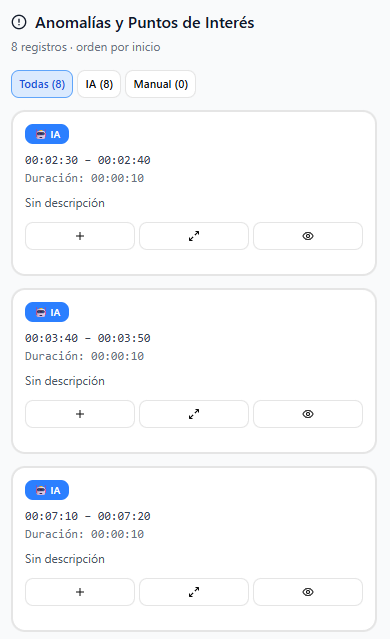
\includegraphics[width=0.55\textwidth]{ThesisFigs/panel_anomalias_ia.png}
    \caption{Panel de anomalías y puntos de interés de EpilexIA con resultados de inteligencia artificial.}
    \label{fig:panel-anomalias-ia}
\end{figure}

La elaboración de informes médicos constituye otra funcionalidad central de este entorno. EpilexIA incorpora una interfaz que permite registrar y actualizar la información correspondiente a la evaluación clínica del estudio. Los formularios se organizan mediante secciones destinadas a documentar los antecedentes y datos clínicos pertinentes, las observaciones sobre el registro electroencefalográfico y las conclusiones del especialista.

La interfaz de informes se encuentra vinculada al estudio EEG correspondiente, lo que facilita la consulta de las señales durante la elaboración del documento. Esta integración permite que el especialista mantenga disponibles los elementos necesarios para relacionar las observaciones realizadas con la información incorporada al informe médico.


El sistema contempla la participación de diferentes Especialistas autorizados en la revisión de un mismo estudio. Cada Especialista puede elaborar un único informe médico propio por estudio, manteniendo diferenciados los registros correspondientes a cada autor. Esta organización permite conservar la individualidad de las evaluaciones y garantiza que ningún Especialista pueda modificar el contenido de un informe perteneciente a otro profesional.


Los informes médicos disponen de estados que permiten distinguir aquellos que se encuentran en Borrador de los que han sido Cerrados. Durante la etapa de borrador, el especialista puede continuar registrando y actualizando la información correspondiente. Una vez cerrado el informe, se aplican las restricciones establecidas por el sistema para impedir modificaciones posteriores.

La presentación de los informes incorpora controles para seleccionar los documentos asociados al estudio y consultar su contenido, de acuerdo con los permisos del usuario. Asimismo, las acciones de creación, edición y cierre se encuentran diferenciadas según el estado del informe y las autorizaciones correspondientes al especialista.

La Figura~\ref{fig:interfaz-informe-medico} presenta la interfaz de elaboración de informes médicos de EpilexIA. En ella se observan las secciones destinadas al registro de información administrativa, datos clínicos, condiciones técnicas, hallazgos ictales e interictales, conclusiones y observaciones. Asimismo, se muestran los controles disponibles para guardar el informe, consultar su vista previa y proceder a su cierre.


\begin{figure}[H]
    \centering

    \begin{minipage}[t]{0.46\textwidth}
        \vspace{0pt}
        \centering
        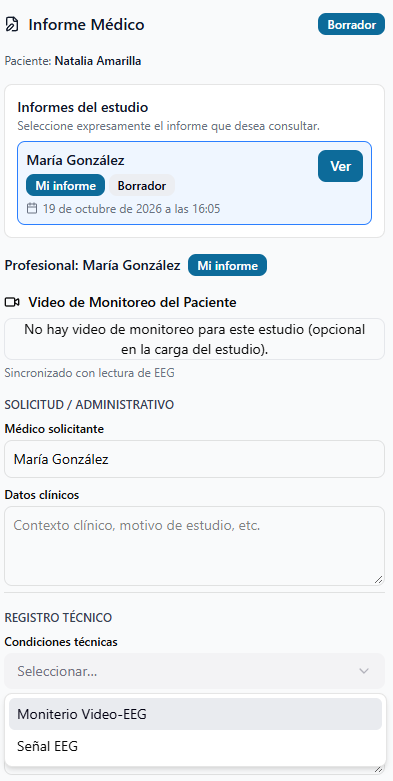
\includegraphics[width=\linewidth]{ThesisFigs/informe_medico_superior.png}
    \end{minipage}
    \hfill
    \begin{minipage}[t]{0.46\textwidth}
        \vspace{0pt}
        \centering
        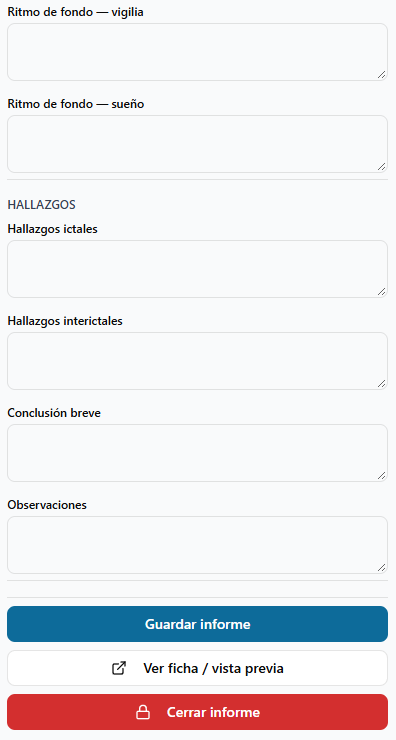
\includegraphics[width=\linewidth]{ThesisFigs/informe_medico_inferior.png}
    \end{minipage}

    \caption{Interfaz de elaboración de informes médicos de EpilexIA.}
    \label{fig:interfaz-informe-medico}
\end{figure}

En conjunto, las interfaces de revisión clínica y elaboración de informes médicos permiten integrar la identificación de hallazgos, el registro de anomalías y eventos, la consulta de resultados de inteligencia artificial y la documentación de las evaluaciones profesionales. Su diseño busca proporcionar un entorno de trabajo organizado que facilite la continuidad entre el análisis de las señales EEG y la elaboración de los informes médicos asociados a cada estudio.

\clearpage
\lhead{\emph{Implementación del sistema}}
\chapter{Implementación del sistema}
\label{cap:implementacion-sistema}

\section{Introducción}
\label{introduccion}

En este capítulo se describe el proceso de implementación del sistema
EpilexIA, desarrollado como una solución informática de apoyo al
análisis de estudios electroencefalográficos y al proceso de diagnóstico
de la epilepsia, mediante la gestión de estudios EEG,
la visualización de señales EEG, la integración de registros de video
y la utilización de técnicas de inteligencia artificial.

La implementación se llevó a cabo a partir de los requerimientos
funcionales y no funcionales, así como de las decisiones arquitectónicas
y de diseño presentadas en el capítulo anterior. Para ello, se utilizaron
tecnologías de código abierto y una organización modular que permite
separar las responsabilidades de la interfaz de usuario, los servicios
de aplicación, la persistencia de datos y los componentes asociados
al procesamiento mediante inteligencia artificial.

\section{Entorno de desarrollo y tecnologías utilizadas}
\label{entorno-desarrollo-tecnologias-utilizadas}

La implementación de EpilexIA se realizó mediante un conjunto de tecnologías y herramientas orientadas al desarrollo de aplicaciones web, la gestión de información clínica y el procesamiento de señales electroencefalográficas mediante inteligencia artificial. La selección de estos componentes permitió organizar el sistema en módulos con responsabilidades diferenciadas, facilitando su desarrollo, integración y mantenimiento.

\subsection{Herramientas y entorno de desarrollo}
\label{herramientas-entorno-desarrollo}

\begin{sloppypar}
\begin{nuevotextodos}
El desarrollo de EpilexIA se organizó mediante cinco repositorios de código fuente: la interfaz web (\texttt{epilexIa-web-front-end}), los servicios de aplicación (\texttt{epilexIa-back-end}), la base de datos clínica (\texttt{epilexIa-database}), la API de inteligencia artificial (\texttt{epilex-ia-api}) y el motor de procesamiento (\texttt{epilex-ia-motor}).
\end{nuevotextodos}
Esta separación permitió administrar de manera diferenciada los componentes del sistema, sus dependencias y sus configuraciones de ejecución.
\end{sloppypar}

Para la verificación del \textit{software}, los repositorios incorporan herramientas de pruebas adaptadas a sus respectivas tecnologías. El \textit{frontend} dispone de Vitest y Testing Library para realizar pruebas sobre componentes y funcionalidades de la interfaz. El \textit{backend} utiliza las herramientas de pruebas de Spring Boot, junto con JUnit, Mockito y Spring Security Test. Los componentes desarrollados en Python incluyen pruebas implementadas mediante el módulo \texttt{unittest}.

\subsection{Tecnologías utilizadas}

La implementación de EpilexIA comprende diferentes tecnologías de
programación, \textit{framework}s y bibliotecas, seleccionadas de acuerdo con
las responsabilidades de cada componente del sistema. Esta organización
permite utilizar herramientas especializadas para la construcción de
la interfaz web, la ejecución de la lógica de negocio, la persistencia
de información y el procesamiento de señales electroencefalográficas
mediante inteligencia artificial.

La interfaz web se desarrolló con React, una biblioteca de JavaScript
orientada a la construcción de interfaces mediante componentes
reutilizables. Para su implementación se utilizó TypeScript, que
incorpora tipado estático al desarrollo de aplicaciones basadas en
JavaScript, junto con Vite como herramienta de desarrollo y
construcción. La navegación entre las diferentes secciones se
implementó mediante React Router, mientras que la comunicación con
los servicios del \textit{backend} se realiza utilizando la API nativa Fetch.

El \textit{backend} se implementó mediante Java 21 y Spring Boot, utilizando
Spring Web MVC para la exposición de servicios REST. La persistencia
de información se gestiona mediante Spring Data JPA e Hibernate,
mientras que Spring Security proporciona los mecanismos de
autenticación y autorización. La aplicación se empaqueta en formato
WAR para su ejecución sobre el servidor de aplicaciones WildFly.

Para el almacenamiento de la información clínica se utiliza
PostgreSQL 17, un sistema gestor de bases de datos relacional. Su
implementación contempla estructuras para almacenar pacientes,
estudios electroencefalográficos, usuarios, informes médicos,
anomalías y otros registros asociados al funcionamiento de EpilexIA.

El subsistema de inteligencia artificial se implementó mediante
Python y se encuentra organizado en dos componentes diferenciados.
El primero corresponde a una API desarrollada con FastAPI, encargada de recibir y gestionar las solicitudes relacionadas con el procesamiento de señales EEG y facilitar la comunicación con los servicios asociados. El segundo corresponde a un motor de procesamiento independiente, responsable de ejecutar las tareas de análisis de las señales electroencefalográficas. Ambos componentes utilizan una instancia PostgreSQL destinada a almacenar información relacionada con las ejecuciones y los resultados del procesamiento.

Para el tratamiento de señales electroencefalográficas se utilizan
bibliotecas científicas como MNE-Python, NumPy, SciPy y pandas.
Asimismo, se emplea joblib para cargar modelos previamente
entrenados y scikit-learn como dependencia necesaria para su
ejecución. Estas herramientas permiten desarrollar las operaciones
de lectura, transformación y procesamiento de datos requeridas
por el subsistema de inteligencia artificial.

Las tecnologías y versiones concretas utilizadas
en la implementación se presentan en el
Cuadro~\ref{tab:tecnologias_epilexia}.

\begingroup
\small
\setlength{\tabcolsep}{3pt}
\renewcommand{\arraystretch}{1.08}
\setlength{\LTleft}{0pt}
\setlength{\LTright}{0pt}

\begin{longtable}{|
p{0.18\dimexpr\textwidth-8\tabcolsep-5\arrayrulewidth\relax}|
p{0.19\dimexpr\textwidth-8\tabcolsep-5\arrayrulewidth\relax}|
p{0.18\dimexpr\textwidth-8\tabcolsep-5\arrayrulewidth\relax}|
p{0.45\dimexpr\textwidth-8\tabcolsep-5\arrayrulewidth\relax}|}

\caption[Principales tecnologías utilizadas en EpilexIA]%
{Tecnologías utilizadas en EpilexIA.}
\label{tab:tecnologias_epilexia}\\
\hline
\textbf{Componente} &
\textbf{Tecnología} &
\textbf{Versión} &
\textbf{Función principal} \\
\hline
\endfirsthead

\multicolumn{4}{c}{\textit{Continuación del Cuadro~\ref{tab:tecnologias_epilexia}}}\\
\hline
\textbf{Componente} &
\textbf{Tecnología} &
\textbf{Versión} &
\textbf{Función principal} \\
\hline
\endhead

\textit{Frontend} & React & 18.3.1 &
Construcción de la interfaz web \\
\hline
\textit{Frontend} & TypeScript & No aplica &
Desarrollo tipado de la interfaz \\
\hline
\textit{Frontend} & Vite & 6.3.5 &
Desarrollo y construcción \\
\hline
\textit{Backend} & Java & 21 &
Implementación de la lógica de negocio \\
\hline
\textit{Backend} & Spring Boot & 3.5.11 &
Desarrollo de servicios de aplicación \\
\hline
\textit{Backend} & WildFly & 39.0.0.Final &
Ejecución de la aplicación \textit{backend} \\
\hline
Base de datos clínica & PostgreSQL & 17 &
Persistencia de información clínica \\
\hline
API de IA & Python & 3.13 &
Implementación de servicios de IA \\
\hline
API de IA & FastAPI & 0.115.6 &
Exposición de servicios de integración \\
\hline
Base de datos de IA & PostgreSQL & 16 &
Persistencia de ejecuciones y resultados \\
\hline
Motor de IA & Python & 3.13 &
Ejecución del procesamiento EEG \\
\hline
Motor de IA & MNE-Python & $\geq$\,\texttt{1.8.0} &
Lectura y procesamiento de señales EEG \\
\hline
Motor de IA & joblib & $\geq$\,\texttt{1.3.0} &
Carga de modelos serializados \\
\hline
Motor de IA & scikit-learn & 1.8.0 &
Ejecución del modelo entrenado \\
\hline

\end{longtable}
\endgroup

Las versiones indicadas corresponden a las dependencias y
configuraciones de los repositorios del proyecto.
En los casos en que se especifican rangos de versiones, la
versión efectiva depende de las dependencias instaladas durante
la construcción de cada componente. 
\begin{nuevotextodos}
TypeScript se utiliza como lenguaje, pero el proyecto no incluye su compilador como dependencia: la conversión a JavaScript la realiza Vite, por lo que no corresponde indicar una versión.
\end{nuevotextodos}

\begin{nuevotexto}
La comparación de las tecnologías alternativas consideradas para cada componente y las herramientas de integración y despliegue se presentan en el Anexo~B.
\end{nuevotexto}

\section{Implementación de la base de datos}

La persistencia de información en EpilexIA se implementó mediante
dos bases de datos PostgreSQL independientes, destinadas a la
gestión de la información clínica y al almacenamiento de los
datos asociados al procesamiento mediante inteligencia
artificial. Esta separación permite organizar los registros
de acuerdo con las responsabilidades de los componentes que
integran el sistema.

La base de datos clínica almacena la información relacionada
con usuarios, pacientes, estudios electroencefalográficos,
archivos asociados, anomalías, informes médicos y registros
de auditoría. Su estructura se implementó mediante \textit{scripts}
SQL y se integra con el \textit{backend} desarrollado en Spring Boot
a través de Spring Data JPA e Hibernate.

Por otra parte, el subsistema de inteligencia artificial
dispone de una base de datos destinada a registrar las
solicitudes de procesamiento, sus estados de ejecución,
los resultados obtenidos y otros datos asociados al análisis
de señales EEG. La persistencia de este componente se
implementó mediante SQLAlchemy, mientras que la evolución
de su esquema se administra principalmente mediante Alembic.

El almacenamiento de los archivos electroencefalográficos
y de video se realiza fuera de las bases de datos, mediante
directorios y volúmenes de almacenamiento. PostgreSQL conserva
las referencias y los metadatos necesarios para relacionar
estos recursos con los estudios correspondientes.

Dado que las bases de datos clínica y de inteligencia
artificial corresponden a instancias PostgreSQL
independientes, no se establecen relaciones de integridad
referencial directas entre sus estructuras. La asociación
de la información se realiza mediante identificadores
de estudios y referencias lógicas utilizadas por los
componentes de aplicación. De esta manera, cada instancia
mantiene su propio esquema y sus mecanismos de persistencia.

Para la adquisición de trabajos pendientes, el
mecanismo de cola utiliza operaciones transaccionales
que permiten seleccionar registros disponibles y
evitar que una misma tarea sea adquirida
simultáneamente por diferentes procesos. Entre
los mecanismos implementados se encuentra el uso
de \texttt{FOR UPDATE SKIP LOCKED}, una cláusula
de PostgreSQL que permite omitir registros
bloqueados durante la selección de tareas.

\begin{nuevotexto}
La arquitectura de persistencia, el esquema de la base de datos clínica y la gestión de los archivos y sus metadatos se detallan en el Anexo~B.
\end{nuevotexto}

\section{Implementación del \textit{backend}}

El \textit{backend} de EpilexIA se implementó utilizando Java 21
y Spring Boot, con el propósito de proporcionar los
servicios de aplicación necesarios para el funcionamiento
del sistema. Este componente concentra las operaciones
de negocio, la gestión del acceso a la información
clínica y los mecanismos de comunicación con la
interfaz web y los servicios asociados.

La implementación se organiza mediante componentes
con responsabilidades diferenciadas, que permiten
separar la recepción de solicitudes, la ejecución
de las operaciones de negocio y el acceso a los
datos persistentes. Para ello, se utilizan
funcionalidades del ecosistema Spring, entre ellas
Spring Web MVC, Spring Data JPA y Spring Security.

Los servicios del \textit{backend} permiten administrar
las operaciones relacionadas con usuarios,
pacientes, estudios electroencefalográficos,
archivos asociados, anomalías, eventos e informes
médicos. Asimismo, incorporan mecanismos de
autenticación y autorización destinados a
controlar el acceso a las funcionalidades
según los permisos asignados a cada usuario.

La aplicación se empaqueta en formato WAR para
su ejecución sobre el servidor de aplicaciones
WildFly. Su integración con los demás componentes
de EpilexIA se realiza mediante interfaces de
comunicación y configuraciones específicas
que permiten coordinar las operaciones del sistema.

\subsection{Organización y estructura del \textit{backend}}

El \textit{backend} de EpilexIA se desarrolló siguiendo una
arquitectura en capas, con una organización que
diferencia las responsabilidades relacionadas con
la recepción de solicitudes, la ejecución de la
lógica de negocio y el acceso a la información
persistente. Esta estructura se implementó mediante
paquetes especializados dentro del proyecto Java,
facilitando la separación de funciones entre los
componentes de la aplicación.

La capa de controladores, organizada en el paquete
\texttt{controller}, se encarga de recibir las
solicitudes HTTP y exponer los servicios REST
utilizados por la interfaz web. Los controladores
delegan las operaciones correspondientes a las
clases del paquete \texttt{service}, donde se
implementan las reglas de negocio, las validaciones
funcionales y la coordinación entre los distintos
componentes del sistema.

\subsection{Implementación de la lógica de negocio}

La lógica de negocio de EpilexIA se implementó
principalmente mediante clases de servicio
desarrolladas con Spring Boot. Estos componentes
se encargan de ejecutar las operaciones
funcionales del sistema, aplicar las reglas
establecidas para cada proceso y coordinar
el acceso a la información persistente.
Esta organización permite mantener las
responsabilidades de negocio diferenciadas
de la recepción de solicitudes HTTP y de
las operaciones de acceso a datos.

La incorporación de archivos EEG se realiza
mediante un mecanismo de carga por fragmentos.
Los servicios comprueban las condiciones
necesarias para recibir los fragmentos,
ensamblan el archivo definitivo y registran
sus referencias y metadatos. Posteriormente,
se inicia el procesamiento asíncrono de
las señales, durante el cual se obtiene
información asociada a los registros EEG
y se actualiza el estado del estudio
según el resultado del procesamiento.

\subsection{Implementación de la autenticación y autorización}

La seguridad del \textit{backend} de EpilexIA se implementó mediante
Spring Security, incorporando mecanismos de autenticación
y autorización para controlar el acceso a las funcionalidades
del sistema. Estos mecanismos permiten identificar a los
usuarios que realizan solicitudes y verificar los permisos
necesarios para ejecutar las operaciones disponibles.

Cuando las credenciales son válidas, el sistema genera un
JWT firmado que contiene el nombre de usuario, un
identificador único de sesión (\texttt{jti}) y las fechas
de emisión y expiración. Los roles y permisos no se
incorporan al \textit{token}, sino que se recuperan desde la base
de datos al procesar las solicitudes autenticadas.

Aunque Spring Security se configuró para no utilizar
sesiones HTTP tradicionales, EpilexIA mantiene registros
persistentes de las sesiones autenticadas. Cada \textit{token}
se vincula con un registro identificado mediante su
\texttt{jti}, cuya existencia y vigencia se comprueban
durante la autenticación de las solicitudes. El cierre
de sesión elimina el registro correspondiente, impidiendo
que el mismo \textit{token} continúe utilizándose. También se
contempla la invalidación de sesiones durante determinados
procesos de restablecimiento de contraseñas.

La autorización se organiza mediante roles y permisos
almacenados en la base de datos. La lógica clínica del
sistema reconoce los perfiles Administrador, Técnico
y Especialista, mientras que las operaciones disponibles
se restringen principalmente mediante permisos
funcionales asociados a los roles correspondientes.

Los controladores REST incorporan restricciones mediante
la anotación \texttt{@PreAuthorize}, que permite comprobar
las autoridades requeridas antes de ejecutar una operación.
Los permisos se representan mediante identificadores
funcionales y se incorporan al contexto de seguridad
a partir de la información recuperada de la base de datos.

Además de estas restricciones generales, determinadas
funcionalidades aplican verificaciones adicionales sobre
los recursos clínicos. En la gestión de estudios, estas
comprobaciones consideran la relación del usuario con
el estudio, incluyendo la asignación de especialistas
y técnicos, así como la participación de observadores.
Para los informes médicos se verifican también la
propiedad del informe y las condiciones establecidas
por su estado y el del estudio asociado.

\subsection{Registro de auditoría y trazabilidad}

El registro de auditoría y trazabilidad de EpilexIA se implementó mediante componentes del \textit{backend} destinados a conservar información sobre determinadas operaciones de negocio realizadas en el sistema. Este mecanismo permite identificar las acciones catalogadas para su seguimiento, registrar el momento de su ejecución y mantener información descriptiva del actor responsable.

La implementación se organiza mediante eventos internos generados durante la ejecución de las operaciones funcionales. Los servicios de aplicación publican eventos cuando se realizan acciones contempladas en el catálogo de auditoría. Estos eventos son recibidos por un componente especializado que se encarga de construir y almacenar los registros correspondientes en la base de datos clínica. Esta organización permite diferenciar la ejecución de las operaciones de negocio del mecanismo encargado de conservar su trazabilidad.

\begin{nuevotexto}
La implementación de los servicios REST, la integración del \textit{backend} con los demás componentes y el diagrama del flujo de autenticación y autorización se presentan en el Anexo~B.
\end{nuevotexto}

\section{Implementación del \textit{frontend}}

El \textit{frontend} de EpilexIA se implementó como una
aplicación web de página única (SPA), utilizando
React 18 y TypeScript, con Vite 6 como herramienta
de desarrollo y construcción. Este componente
constituye la interfaz de interacción entre los
usuarios y las funcionalidades clínicas, técnicas
y administrativas del sistema.

La organización del código se basa en una
estructura modular que distingue las páginas,
las funcionalidades del dominio, los componentes
compartidos y la configuración general de la
aplicación. Para la administración del estado
se emplean mecanismos nativos de React y
contextos especializados, mientras que la
comunicación con el \textit{backend} se realiza mediante
solicitudes HTTP a los servicios REST.

La interfaz permite gestionar estudios
electroencefalográficos y sus pacientes
asociados, cargar archivos EEG y video,
visualizar señales EEG y consultar resultados de inteligencia artificial, elaborar informes médicos y
acceder a funcionalidades administrativas
según los permisos del usuario.

\subsection{Arquitectura, tecnologías y organización del código}

La implementación del \textit{frontend} sigue una arquitectura
de aplicación de página única, en la cual React se
encarga de construir y actualizar las interfaces
mediante componentes reutilizables. TypeScript
permite definir tipos para los datos, las propiedades
de los componentes y las respuestas de los servicios,
mientras que Vite proporciona las herramientas
necesarias para el desarrollo y la generación de
los archivos de distribución de la aplicación.

La administración del estado se realiza principalmente
mediante mecanismos nativos de React, como
\texttt{useState}, \texttt{useReducer},
\texttt{useRef} y \texttt{useEffect}.
Para compartir información entre componentes
se utilizan contextos especializados.
Entre ellos se encuentran \texttt{AuthProvider},
responsable de mantener los datos de autenticación
y permisos del usuario, y
\texttt{UploadProgressProvider}, que permite
conservar el estado de las transferencias de
archivos mientras se navega entre las páginas
de la aplicación.

\subsection{Navegación, autenticación y gestión de interfaces}

La navegación del \textit{frontend} se implementó mediante
React Router DOM, utilizando el componente
\texttt{BrowserRouter} para administrar las rutas
de la aplicación sin requerir la recarga completa
de la página en cada transición. La configuración
del enrutamiento se encuentra centralizada en
\texttt{src/app/router.tsx}, donde se definen
las rutas públicas y aquellas que requieren
una sesión autenticada.

La gestión de la sesión se centraliza mediante
\texttt{AuthProvider}, que mantiene la información
del usuario autenticado y sus permisos. El \textit{frontend}
conserva el \textit{token} JWT y los datos necesarios para
restaurar la sesión en el almacenamiento local del
navegador (\texttt{localStorage}). Este mecanismo
permite recuperar la sesión al volver a cargar la
aplicación. No obstante, el almacenamiento de \textit{tokens}
en este medio requiere considerar los riesgos asociados
a la ejecución de \textit{scripts} maliciosos en el navegador,
por lo que constituye un aspecto de seguridad
susceptible de revisión en futuras versiones del sistema.

\subsection{Gestión integrada de pacientes y estudios EEG}

Durante el registro de un nuevo estudio,
el usuario puede buscar pacientes previamente
registrados mediante un campo de búsqueda
que consulta los resultados de forma diferida,
reduciendo la cantidad de solicitudes realizadas
mientras se introduce el texto. A partir de
los resultados obtenidos, es posible seleccionar
al paciente correspondiente y asociarlo al
estudio que se está creando.

\subsection{Carga y seguimiento de archivos EEG y video}

Para la transferencia de archivos EEG se
utiliza un mecanismo de carga por fragmentos,
implementado mediante una utilidad compartida.
El archivo seleccionado se divide en partes
de tamaño configurable, que posteriormente
se envían al servidor mediante solicitudes
HTTP. Este procedimiento permite organizar
la transferencia sin requerir el envío
del archivo completo en una única solicitud.

Una vez enviados los fragmentos, el \textit{frontend}
realiza la solicitud de confirmación de la
carga y consulta periódicamente el estado
del procesamiento del archivo EEG. Este
seguimiento permite identificar la evolución
de las tareas ejecutadas por el \textit{backend},
sin bloquear la interfaz durante el
procesamiento asíncrono de las señales.

\subsection{Implementación del visualizador EEG}

El visualizador EEG constituye uno de los
componentes principales de la interfaz web
de EpilexIA, al proporcionar las herramientas
necesarias para examinar las señales
electroencefalográficas asociadas a un estudio.
Su implementación integra la representación
gráfica de los canales, la navegación temporal,
la configuración de montajes y filtros, y
la interacción con las anomalías y eventos
registrados durante el análisis.

La representación de las señales se realiza
mediante el componente \texttt{EegStackedChart},
desarrollado con elementos gráficos SVG
(Scalable Vector Graphics). Este componente
construye las trayectorias correspondientes
a las muestras de cada canal y las dispone
de forma apilada, permitiendo visualizar
simultáneamente las distintas derivaciones
electroencefalográficas. A diferencia de
otros gráficos presentes en la aplicación,
el trazado EEG utiliza una implementación
SVG propia, sin depender de la biblioteca
Recharts para representar las señales.

Las muestras necesarias para la visualización
se obtienen mediante solicitudes al \textit{backend},
delimitadas por intervalos temporales.
El \textit{frontend} administra la ventana de tiempo
visible y proporciona controles para avanzar,
retroceder, modificar la escala temporal
y desplazar el cursor sobre las señales.
Asimismo, incorpora mecanismos de caché
y precarga de segmentos para reutilizar
información previamente obtenida y facilitar
la navegación entre diferentes intervalos
del registro.

El visualizador dispone de controles para configurar las frecuencias de corte inferior (\textit{Low cut}) y superior (\textit{High cut}), así como un filtro de rechazo de banda (\texttt{notch}) de 50 Hz. También incorpora configuraciones
predefinidas y ajustes individuales por
canal. Antes de enviar los parámetros,
la interfaz comprueba condiciones como
la utilización de valores positivos,
la relación entre las frecuencias de
corte y el límite establecido por la
frecuencia de Nyquist.

\subsection{Reproducción sincronizada de video y presentación de resultados de IA}

La sincronización entre las señales
EEG y el video se establece mediante
una referencia temporal compartida.
Durante la navegación por el registro,
la interfaz relaciona la posición
temporal de las señales con el instante
correspondiente del video, de modo
que ambas representaciones puedan
examinarse dentro de un mismo contexto
de análisis.

En relación con la inteligencia
artificial, el \textit{frontend} incorpora
interfaces para solicitar el análisis
de un estudio y consultar el estado
de su ejecución. Debido a que el
procesamiento se desarrolla de manera
asíncrona, la aplicación realiza
consultas periódicas a los servicios
correspondientes para obtener
información actualizada sobre
su evolución y finalización.

\subsection{Elaboración y consulta de informes médicos}

La elaboración de informes médicos se implementó
mediante una interfaz integrada al visualizador
de estudios EEG, que permite a los especialistas
registrar y consultar las observaciones clínicas
derivadas del análisis electroencefalográfico.
Esta funcionalidad vincula la exploración de las
señales con la documentación de los resultados
correspondientes a cada estudio.

\begin{nuevotexto}
La administración de usuarios, la consulta de auditoría y el esquema funcional del visualizador se describen en el Anexo~B.
Las pruebas automatizadas del \textit{frontend} se resumen en la Sección~\ref{sec:pruebas-automatizadas}.
\end{nuevotexto}

\section{Implementación de los componentes de inteligencia artificial}

La implementación de los componentes de inteligencia artificial
de EpilexIA comprende los servicios encargados de gestionar
las solicitudes de análisis electroencefalográfico, ejecutar
los procedimientos de procesamiento de señales y poner a
disposición los resultados obtenidos. Estos componentes
complementan las funcionalidades del sistema clínico mediante
mecanismos de análisis automatizado que proporcionan
información de apoyo para la evaluación de los estudios EEG.

La solución se organiza en dos componentes principales:
una interfaz de servicios desarrollada con FastAPI y un
motor independiente de procesamiento implementado en Python.
Esta separación permite distinguir las responsabilidades
de comunicación, validación y gestión de ejecuciones de
las operaciones de procesamiento científico e inferencia.

La coordinación entre ambos componentes se realiza mediante
una base de datos PostgreSQL, utilizada tanto para conservar
la información de las ejecuciones como para gestionar una
cola persistente de trabajos. De esta manera, las solicitudes
de análisis pueden registrarse y consultarse sin requerir
que el procesamiento intensivo se complete durante la
atención de una petición HTTP.

\subsection{Arquitectura y organización de los componentes de inteligencia artificial}

\begin{nuevotextodos}
La API de inteligencia artificial, desarrollada con FastAPI, recibe y valida las solicitudes, administra las ejecuciones y permite consultar sus estados y resultados.
Accede a la base de datos mediante SQLAlchemy y administra los cambios del esquema con migraciones de Alembic.
El motor es un proceso independiente, también desarrollado en Python, que no expone una interfaz HTTP: recupera los trabajos pendientes, ejecuta el procesamiento electroencefalográfico y registra los resultados y los estados de las ejecuciones.
El diagrama de estos componentes se presenta en el Anexo~B.
\end{nuevotextodos}

\subsection{Implementación de la API de inteligencia artificial}

Entre las funcionalidades principales se
encuentra el registro de nuevas ejecuciones
de inteligencia artificial asociadas a un
estudio EEG. Al recibir una solicitud, la API
comprueba los datos requeridos y registra
la información necesaria para administrar
el procesamiento. La solicitud incorpora
la identificación del estudio y los parámetros
admitidos por el servicio, mientras que
la ejecución del análisis se desarrolla
posteriormente, mediante la cola de ejecuciones.

\subsection{Gestión asíncrona de ejecuciones y coordinación con el motor}

La coordinación entre la API de inteligencia
artificial y el motor independiente se realiza
mediante una cola persistente implementada
sobre PostgreSQL. Cuando se solicita el análisis
de un estudio, la API registra la ejecución
y la información necesaria para su procesamiento.
Posteriormente, el motor consulta la base
de datos para identificar los trabajos
pendientes y comenzar su ejecución.

El mecanismo de recuperación de trabajos
utiliza operaciones transaccionales sobre
PostgreSQL, incluyendo la cláusula
\texttt{FOR UPDATE SKIP LOCKED}. Esta
instrucción permite seleccionar y bloquear
registros disponibles, omitiendo aquellos
que ya se encuentran bloqueados por otras
transacciones. Su utilización contribuye
a coordinar la reserva de trabajos cuando
existen procesos que consultan la misma
cola, reduciendo la posibilidad de que
un trabajo sea reservado simultáneamente
por más de un trabajador.

\subsection{Integración del modelo de detección}
\label{subsec:modelo-vigente-hgb}

El modelo de detección y el procedimiento de análisis que lo acompaña fueron desarrollados por el equipo de ciencia de datos del proyecto EpilexIA.
El presente trabajo no comprende su diseño ni su entrenamiento, sino su integración en el motor y en la plataforma.
Por ello, esta subsección describe el procedimiento únicamente en el nivel necesario para explicar dicha integración.

Al iniciar una ejecución, el motor recupera la ruta relativa del archivo EEG almacenada en el campo \texttt{edf\_path} de la tabla \texttt{ai\_executions} y la combina con la ruta base del volumen configurado.
Antes de comenzar el análisis, comprueba la existencia del archivo EDF y del paquete del modelo.

\begin{nuevotextodos}
El modelo vigente, denominado HGB~2.0, es un clasificador de \textit{Gradient Boosting} basado en histogramas (\textit{Histogram-based Gradient Boosting}, HGB), en línea con los antecedentes desarrollados en la FP-UNA \citep{Lezcano2026GradientBoosting}.
Analiza el registro en ventanas consecutivas de 10 segundos y señala un intervalo cuando dos ventanas seguidas superan un umbral de probabilidad de 0,95.
Las etapas previas del procedimiento (lectura, montaje, filtrado, segmentación, cálculo de características y normalización) se describen en el Anexo~B.
\end{nuevotextodos}

El motor invoca este procedimiento para cada ejecución, indicando el archivo EDF, el paquete del modelo y el archivo de salida.
El paquete serializado del modelo incluye la configuración de preprocesamiento con la que fue entrenado.
Antes de ejecutar la inferencia, el motor verifica que la frecuencia de muestreo, la duración de las ventanas, las derivaciones y las características coincidan con dicha configuración, y aborta la ejecución en caso contrario.
El umbral y la cantidad de ventanas consecutivas se obtienen del paquete del modelo y pueden establecerse para cada ejecución; el umbral aplicado queda registrado junto con la ejecución.

Como salida, el procedimiento genera un archivo con una fila por cada ventana analizada.
Los resultados se almacenan por ventana: cada ventana de diez segundos que integra una secuencia señalada se registra como un resultado individual, de modo que una detección de 20 segundos se presenta como dos registros consecutivos.

\subsection{Evolución del modelo de detección}
\label{subsec:evolucion-modelo}

La integración se realizó inicialmente con una primera versión del modelo, identificada como MLP, que permitió construir y probar el circuito completo del sistema: la solicitud del análisis, la cola de ejecuciones, el procesamiento y la presentación de los resultados.
Durante el proyecto, el equipo de ciencia de datos continuó el desarrollo de sus modelos y proporcionó la versión HGB~2.0, que reemplazó a la anterior.
Todas las pruebas finales documentadas en el Capítulo~\ref{pruebas_evaluacion} se realizaron con este modelo.

El reemplazo requirió adaptar el motor al nuevo procedimiento de análisis, sin modificaciones en la comunicación con el \textit{backend} clínico ni en la interfaz web.
Dado que cada modelo se distribuye como un paquete que incluye su propia configuración, el sistema queda preparado para incorporar las versiones posteriores que resulten de la continuidad de esa línea de trabajo.

\subsection{Generación de espectrogramas DSA}

La implementación de EpilexIA incorpora la generación de
espectrogramas DSA como
una herramienta complementaria para la visualización y el
análisis de las señales electroencefalográficas. Esta
funcionalidad permite representar la evolución temporal
del contenido frecuencial de un registro EEG, facilitando
la identificación visual de variaciones en su actividad
espectral.

La generación de espectrogramas se encuentra implementada
en la API de inteligencia artificial, mediante un servicio
de procesamiento espectral independiente del motor de
clasificación de crisis. A diferencia de las ejecuciones
de inferencia, este procedimiento se realiza bajo demanda,
sin utilizar la cola persistente de trabajos ni el motor.

La solicitud se origina en la interfaz web y se transmite
al \textit{backend} clínico mediante un servicio REST asociado al
estudio EEG. El \textit{backend} comprueba la existencia del estudio,
verifica que disponga de un archivo EDF y construye la
solicitud correspondiente a la API de inteligencia
artificial. Esta última recibe los parámetros de selección
de canales, referencia y límites temporales, y ejecuta
el procesamiento necesario para generar la representación
espectral.

\begin{figure}[htbp]
    \centering
    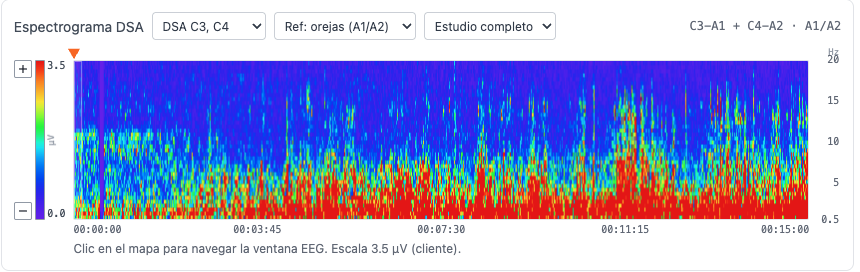
\includegraphics[width=\textwidth]{Chapter5/chapter5Figs/espectrograma_dsa.png}
    \caption{Visualización del espectrograma DSA
    implementado en EpilexIA.}
    \label{fig:espectrograma_dsa}
\end{figure}

\begin{nuevotexto}
La persistencia y la consulta de los resultados, el cálculo de los espectrogramas y las limitaciones de la implementación se detallan en el Anexo~B.
Las pruebas automatizadas de la API y del motor se resumen en la Sección~\ref{sec:pruebas-automatizadas}.
\end{nuevotexto}

\section{Despliegue e integración de los componentes}

El despliegue de EpilexIA comprende la configuración y puesta en
funcionamiento de los componentes que conforman el sistema, así
como el establecimiento de los mecanismos necesarios para su
comunicación y acceso a los recursos compartidos. La implementación
se organiza en proyectos independientes que incluyen la interfaz
web, el \textit{backend} clínico, la base de datos clínica, la API de
inteligencia artificial y el motor de procesamiento.

Para facilitar la construcción y ejecución de estos componentes,
se utilizan contenedores Docker y archivos de configuración
Docker Compose. Esta organización permite definir las dependencias
de ejecución, los puertos de comunicación, las variables de
entorno y los recursos de almacenamiento necesarios para cada
servicio.

La integración se realiza mediante una red Docker compartida,
servicios HTTP y mecanismos de persistencia. Asimismo, se
emplean volúmenes para conservar la información de las bases
de datos y permitir el acceso a los archivos electroencefalográficos
y a los modelos de clasificación.

\subsection{Entorno de despliegue en la nube}
\label{subsec:despliegue-nube}

EpilexIA se encuentra desplegado en infraestructura en la nube provista por la empresa BigQ, socio del sector privado del proyecto.
Sobre este entorno se realizaron las pruebas documentadas en el Capítulo~\ref{pruebas_evaluacion} y las sesiones de validación con la especialista del IPS, quien accede al sistema por internet desde el hospital.

El despliegue reúne en un servidor los componentes del sistema, ejecutados como contenedores mediante una configuración conjunta de Docker Compose.
Un servidor Nginx actúa como punto único de entrada: publica la aplicación web y encamina las solicitudes hacia el \textit{backend} clínico.
Las bases de datos, la API de inteligencia artificial y el motor de procesamiento no se exponen a internet y se comunican únicamente a través de una red interna.
Los archivos EEG y los modelos entrenados se almacenan en volúmenes compartidos entre los servicios que los requieren.

El acceso de los usuarios se realiza mediante HTTPS, bajo un dominio provisto por la empresa, cuya infraestructura incorpora además mecanismos de protección perimetral.
De este modo se atiende el requerimiento RNF-SEG-003.
La administración de estos elementos corresponde al proveedor de infraestructura y no forma parte del alcance de este trabajo.

Este entorno constituye la base operativa del sistema durante el proceso de transferencia al IPS, que prevé su despliegue en servidores propios de la institución.

\subsection{Contenedorización y configuración de servicios}

La contenedorización de los componentes de EpilexIA se implementa
mediante Docker, utilizando archivos \texttt{Dockerfile} para definir los
entornos de ejecución y configuraciones Docker Compose para
administrar los servicios asociados a cada proyecto. Esta
organización permite establecer las dependencias necesarias,
los comandos de inicio, las variables de entorno y los recursos
requeridos para el funcionamiento de las aplicaciones.

El Cuadro~\ref{tab:componentes-contenedorizados} resume los
principales componentes de ejecución de EpilexIA, indicando
las tecnologías utilizadas y las responsabilidades que
cumplen dentro del entorno contenedorizado.

\begin{table}[htbp]
    \centering
    \caption{Componentes contenedorizados del sistema EpilexIA.}
    \label{tab:componentes-contenedorizados}
    \small
    \begin{tabularx}{\textwidth}{|
        >{\raggedright\arraybackslash}p{0.27\textwidth}|
        >{\raggedright\arraybackslash}p{0.27\textwidth}|
        >{\raggedright\arraybackslash}X|}
        \hline
        \textbf{Componente} &
        \textbf{Entorno de ejecución} &
        \textbf{Responsabilidad principal} \\
        \hline

        \textit{Frontend} &
        Node.js (compilación) y Nginx (ejecución) &
        Compilación y publicación de la interfaz web. \\
        \hline

        \textit{backend} clínico &
        Java 21 y WildFly 39 &
        Ejecución de los servicios clínicos y las operaciones de negocio. \\
        \hline

        Base de datos clínica &
        PostgreSQL 17 &
        Almacenamiento persistente de la información clínica. \\
        \hline

        API de inteligencia artificial &
        Python, FastAPI y Uvicorn &
        Recepción de solicitudes y administración de ejecuciones y resultados. \\
        \hline

        Base de datos de inteligencia artificial &
        PostgreSQL 16 &
        Persistencia de ejecuciones, cola de trabajos y resultados del análisis. \\
        \hline

        Motor de inteligencia artificial &
        Python &
        Procesamiento de señales EEG y ejecución del modelo de clasificación. \\
        \hline
    \end{tabularx}
\end{table}

\subsection[Consideraciones operativas y limitaciones del despliegue]{Consideraciones operativas y limitaciones del \\despliegue}

En cuanto a las limitaciones del despliegue, el despliegue se encuentra distribuido entre
configuraciones Docker Compose individuales y una configuración conjunta utilizada en la nube.
No se dispone de un procedimiento único y completamente automatizado que abarque la preparación de todos los recursos, la inicialización de los servicios y la verificación integral de su funcionamiento.

Por otra parte, la utilización de una cola persistente
permite desacoplar la recepción de solicitudes de
inteligencia artificial de la ejecución de los trabajos.
Sin embargo, la disponibilidad del procesamiento
automatizado depende de que el motor se encuentre en
funcionamiento y pueda acceder tanto a la base de datos
de inteligencia artificial como a los archivos necesarios
para realizar el análisis.

Finalmente, no se evaluaron la escalabilidad, la tolerancia
a fallos ni el comportamiento del sistema bajo cargas elevadas.
La evaluación de estas propiedades requiere pruebas
específicas y condiciones de ejecución definidas,
que deben distinguirse de la descripción de los
mecanismos de contenedorización implementados.

\begin{nuevotexto}
La configuración de cada contenedor, las consideraciones operativas para la puesta en funcionamiento y la comunicación entre los componentes desplegados se detallan en el Anexo~B.
\end{nuevotexto}



\clearpage
\lhead{\emph{Pruebas y evaluación}}

\chapter{Pruebas y evaluación}
\label{pruebas_evaluacion}

\section{Estrategia de pruebas}
\label{sec:estrategia_pruebas}

La estrategia de pruebas y evaluación de EpilexIA se orienta a verificar el comportamiento funcional del sistema, la integración entre sus componentes, el procesamiento y la visualización de señales electroencefalográficas, así como su rendimiento y usabilidad en el contexto de aplicación previsto. Para ello, se consideran procedimientos de verificación técnica y actividades de evaluación con usuarios, con el propósito de obtener evidencias sobre el cumplimiento de los requerimientos establecidos.

Se adopta principalmente un enfoque de pruebas de caja negra, mediante el cual se evalúa el comportamiento observable del sistema a partir de las entradas proporcionadas y las salidas obtenidas, sin requerir el conocimiento de los detalles internos de implementación. Este enfoque permite analizar EpilexIA desde la perspectiva de sus usuarios y de los servicios que ofrece, considerando operaciones como la gestión de pacientes y estudios, la carga de archivos EEG, la visualización de señales, el registro de anomalías, la ejecución del análisis mediante inteligencia artificial y la elaboración de informes médicos.

La estrategia contempla los siguientes ámbitos de evaluación:

\begin{itemize}
    \item \textbf{Pruebas funcionales:} orientadas a comprobar que las funcionalidades del sistema respondan a los requerimientos definidos y produzcan los resultados esperados ante diferentes condiciones de utilización.

    
    \item \textbf{Pruebas de integración:} destinadas a verificar la comunicación y el intercambio de información entre el \textit{frontend}, el \textit{backend}, las bases de datos y los componentes de inteligencia artificial.

    \item \textbf{Pruebas de procesamiento y visualización EEG:} enfocadas en evaluar la carga y representación de señales, la configuración de montajes, filtros y sensibilidad, la navegación temporal y el registro de anomalías. Sus resultados se presentan en los casos PF-05 a PF-09 y en la prueba de integración PI-05.

    \item \textbf{Pruebas de integración con inteligencia artificial:} dirigidas a comprobar la solicitud de análisis, el seguimiento de las ejecuciones y la recuperación y presentación de los resultados generados.

    \item \textbf{Pruebas de rendimiento:} previstas en la estrategia y no ejecutadas en el presente trabajo, destinadas a medir indicadores cuantitativos, como los tiempos de respuesta, la duración de las operaciones, el consumo de recursos computacionales y el comportamiento del sistema bajo diferentes condiciones de carga.

    \item \textbf{Evaluación de usabilidad:} realizada de forma exploratoria y cualitativa, orientada a analizar la eficacia, eficiencia y satisfacción de los usuarios al realizar tareas representativas de su actividad, considerando como referencia los principios establecidos en la norma ISO~9241-11.
\end{itemize}

Para las pruebas funcionales y de integración se utilizaron casos de prueba que especifican la funcionalidad evaluada, el procedimiento de ejecución y el resultado esperado. Las condiciones de cada ejecución y el resultado obtenido se documentan en la sección correspondiente a cada prueba. Esta estructura permitió documentar los comportamientos observados e identificar posibles diferencias respecto de los requerimientos del sistema.

Las pruebas de integración con el servicio de inteligencia artificial y las sesiones con la especialista se ejecutaron sobre la instancia del sistema desplegada en la nube, descrita en la Sección~\ref{subsec:despliegue-nube}.

La evaluación contó con la participación de una médica especialista en epileptología del Hospital Central del Instituto de Previsión Social (IPS), quien accedió a la instancia de EpilexIA desplegada en la infraestructura en la nube de BigQ (Sección~\ref{subsec:despliegue-nube}) desde las instalaciones hospitalarias, utilizando una cuenta individual con el perfil Especialista. Durante su utilización, la profesional comunicó verbalmente observaciones y sugerencias que fueron registradas por el equipo de desarrollo. Estas observaciones dieron lugar a un conjunto de mejoras funcionales, principalmente relacionadas con el visualizador EEG y las herramientas de análisis, que se detallan en el Cuadro~\ref{tab:observaciones-especialista}. Esta actividad se considera una evaluación exploratoria, dado que no incluyó la aplicación de cuestionarios estandarizados ni la medición sistemática de indicadores de usabilidad.

Finalmente, las evidencias obtenidas servirán de base para analizar el cumplimiento de los requerimientos funcionales y no funcionales, así como para valorar los resultados del sistema en relación con los objetivos y la hipótesis planteados en la investigación.

\section{Pruebas funcionales}
\label{sec:pruebas_funcionales}

\begin{nuevotexto}
Las pruebas funcionales verificaron que las operaciones disponibles en EpilexIA respondan a los requerimientos establecidos.
Siguen el flujo de trabajo clínico: la autenticación, el registro de pacientes y estudios, la revisión de las señales, la consulta de los resultados de inteligencia artificial, la elaboración de informes y la auditoría.
Se definieron quince casos, identificados de PF-01 a PF-15, cada uno con su procedimiento y su resultado esperado.
Todos se ejecutaron sobre la interfaz web, con cuentas de los perfiles correspondientes.

El Cuadro~\ref{tab:sintesis_pruebas_funcionales} resume, para cada caso, la verificación realizada y el resultado obtenido.
El procedimiento completo de cada prueba y sus evidencias se presentan en el Anexo~C.

\begingroup
\small
\setlength{\tabcolsep}{4pt}
\renewcommand{\arraystretch}{1.15}
\begin{longtable}{|p{1.25cm}|p{3.4cm}|p{7.6cm}|p{1.75cm}|}
\caption{Resultados de las pruebas funcionales de EpilexIA.}
\label{tab:sintesis_pruebas_funcionales}\\
\hline
\textbf{ID} & \textbf{Funcionalidad} & \textbf{Verificación realizada y resultado observado} & \textbf{Resultado} \\
\hline
\endfirsthead
\multicolumn{4}{c}{\textit{Continuación del Cuadro \thetable}}\\
\hline
\textbf{ID} & \textbf{Funcionalidad} & \textbf{Verificación realizada y resultado observado} & \textbf{Resultado} \\
\hline
\endhead

PF-01 &
Autenticación de usuarios &
Inicio de sesión con credenciales válidas. El sistema presentó el panel de control con las opciones del perfil Especialista. &
Aprobada \\
\hline

PF-02 &
Validación de credenciales &
Inicio de sesión con una contraseña incorrecta. El sistema mostró el mensaje «Credenciales inválidas» e impidió el acceso. &
Aprobada \\
\hline

PF-03 &
Registro de pacientes &
Registro de un paciente ficticio y búsqueda posterior. El paciente quedó disponible para su selección al crear un estudio. &
Aprobada \\
\hline

PF-04 &
Registro de estudios EEG &
Creación de un estudio asociado al paciente, con validación previa del archivo. El estudio figuró en el listado con estado Procesado. &
Aprobada \\
\hline

PF-05 &
Carga de archivos EEG &
Carga de un archivo EDF junto con el estudio. El sistema mostró el progreso de la transferencia y el estado final Procesado. &
Aprobada \\
\hline

PF-06 &
Visualización de señales EEG &
Apertura del estudio en el visualizador. Se presentaron las señales con sus canales y referencias temporales, y la sensibilidad se ajustó entre 100~$\mu$V y 5~$\mu$V. &
Aprobada \\
\hline

PF-07 &
Configuración de montajes &
Cambio entre los montajes Doble Banana y Transversal sobre un mismo intervalo. El sistema actualizó las derivaciones presentadas. &
Aprobada \\
\hline

PF-08 &
Configuración de filtros &
Modificación del corte inferior (1~Hz y 0,5~Hz), del corte superior (70~Hz y 30~Hz) y del filtro de red. La señal se actualizó en cada caso. &
Aprobada \\
\hline

PF-09 &
Registro manual de anomalías &
Marcado de un intervalo de nueve segundos y guardado como anomalía. El registro quedó disponible en el panel de anomalías. &
Aprobada \\
\hline

PF-10 &
Consulta de resultados de IA &
Consulta del panel de anomalías de un estudio analizado: 47 registros, 43 generados mediante IA y 4 manuales, distinguibles por su origen. Desde cada registro se accedió al intervalo correspondiente. &
Aprobada \\
\hline

PF-11 &
Elaboración de informes médicos &
Redacción y guardado de un informe en estado Borrador. El contenido se conservó al volver a consultar el estudio. &
Aprobada \\
\hline

PF-12 &
Restricción de edición de informes &
Consulta del informe de otro especialista. El sistema lo presentó en modo de solo lectura. &
Aprobada \\
\hline

PF-13 &
Cierre de informes médicos &
Cierre de un informe, con confirmación previa. El informe pasó al estado Cerrado y no admitió modificaciones, tampoco después de reiniciar la sesión. &
Aprobada \\
\hline

PF-14 &
Control de acceso según perfil &
Ingreso con cuentas de los tres perfiles. Cada una presentó únicamente las opciones que le corresponden: gestión de usuarios para el Administrador, estudios para el Técnico, y estudios y reportes para el Especialista. &
Aprobada \\
\hline

PF-15 &
Consulta de auditoría &
Consulta del historial de auditoría con filtros por fecha, evento, actor y rol. El sistema presentó los registros correspondientes a cada filtro. &
Aprobada \\
\hline

\end{longtable}
\endgroup

Los quince casos resultaron aprobados: en todos, el comportamiento observado coincidió con el esperado.
Estas pruebas verifican la disponibilidad y el funcionamiento de las operaciones desde la perspectiva de los usuarios.
No evalúan la precisión diagnóstica del modelo ni constituyen una validación integral de la seguridad o del rendimiento, aspectos que se tratan en la Sección~\ref{sec:sintesis-aspectos}.
\end{nuevotexto}

\section{Pruebas de integración}
\label{sec:pruebas_integracion}

\begin{nuevotexto}
Las pruebas de integración verificaron la comunicación entre los componentes del sistema: la interfaz web, el \textit{backend} clínico, las bases de datos, la API de inteligencia artificial y el motor de procesamiento.
A diferencia de las pruebas funcionales, en cada caso se comprobó, además del comportamiento visible en la interfaz, la respuesta de los servicios y el estado almacenado en las bases de datos.

Se definieron diecisiete casos, identificados de PI-01 a PI-17.
Los casos PI-01 a PI-05 corresponden a la autenticación, las sesiones y la persistencia de pacientes y estudios.
Los casos PI-06 a PI-14 corresponden al ciclo de procesamiento mediante inteligencia artificial.
Los casos PI-15 y PI-16 evalúan el comportamiento ante fallos, y el caso PI-17, la sincronización de la información de los informes médicos con el subsistema de IA.

Los casos PI-15 y PI-16 requieren detener servicios de manera deliberada.
Por ello se ejecutaron en un entorno de pruebas local, que replica el despliegue mediante los mismos contenedores, para no afectar la instancia utilizada en el hospital.

El Cuadro~\ref{tab:resumen_pruebas_integracion} resume la verificación realizada y el resultado obtenido en cada caso.
El procedimiento de cada prueba y sus evidencias, que incluyen las respuestas de los servicios y las consultas a las bases de datos, se presentan en el Anexo~C.

\begingroup
\small
\setlength{\tabcolsep}{4pt}
\renewcommand{\arraystretch}{1.15}
\begin{longtable}{|p{1.25cm}|p{3.4cm}|p{7.6cm}|p{1.75cm}|}
\caption{Resultados de las pruebas de integración de EpilexIA.}
\label{tab:resumen_pruebas_integracion}\\
\hline
\textbf{ID} & \textbf{Integración evaluada} & \textbf{Verificación realizada y resultado observado} & \textbf{Resultado} \\
\hline
\endfirsthead
\multicolumn{4}{c}{\textit{Continuación del Cuadro \thetable}}\\
\hline
\textbf{ID} & \textbf{Integración evaluada} & \textbf{Verificación realizada y resultado observado} & \textbf{Resultado} \\
\hline
\endhead

PI-01 &
Autenticación de usuarios &
El inicio de sesión devolvió un \textit{token} JWT, las solicitudes protegidas respondieron con el código HTTP 200 y la sesión quedó registrada en la base de datos. &
Aprobada \\
\hline

PI-02 &
Protección de servicios &
Una solicitud sin \textit{token} recibió el código HTTP 401, sin datos clínicos. El acceso directo al panel de control sin sesión se redirigió al inicio de sesión. &
Aprobada \\
\hline

PI-03 &
Revocación de sesiones &
Después del cierre de sesión, una solicitud con el mismo \textit{token} recibió el código HTTP 401. &
Aprobada \\
\hline

PI-04 &
Persistencia de pacientes &
El paciente registrado desde la interfaz se recuperó, con los mismos datos, mediante una consulta directa a la base de datos. &
Aprobada \\
\hline

PI-05 &
Registro de estudios y archivos EEG &
El estudio, el archivo EDF y sus metadatos (tamaño, duración y frecuencia de muestreo) quedaron almacenados y asociados, y las señales se visualizaron. &
Aprobada \\
\hline

PI-06 &
Creación de ejecuciones de IA &
Cada solicitud de análisis generó una ejecución identificable, registrada en las dos bases de datos. &
Aprobada \\
\hline

PI-07 &
Prevención de ejecuciones duplicadas &
Una nueva solicitud para un estudio con una ejecución activa no generó un trabajo adicional. &
Aprobada \\
\hline

PI-08 &
Recuperación de trabajos pendientes &
El motor tomó los trabajos en cola y actualizó su estado al iniciar el procesamiento. &
Aprobada \\
\hline

PI-09 &
Actualización de actividad del motor &
La señal de actividad del motor se actualizó periódicamente durante el procesamiento. &
Aprobada \\
\hline

PI-10 &
Propagación del estado de ejecución &
Los cambios de estado de la ejecución se reflejaron en la interfaz web. &
Aprobada \\
\hline

PI-11 &
Recuperación de resultados de IA &
Los resultados presentados en la interfaz correspondieron a la ejecución consultada. &
Aprobada \\
\hline

PI-12 &
Inicio automático de ejecuciones &
Los estudios procesados que no contaban con análisis se encolaron de forma automática. &
Aprobada \\
\hline

PI-13 &
Generación de espectrogramas &
El servicio devolvió los datos del espectrograma y la interfaz los presentó. &
Aprobada \\
\hline

PI-14 &
Registro de eventos de IA &
Los eventos del ciclo de ejecución quedaron registrados y pudieron consultarse en la auditoría. &
Aprobada \\
\hline

PI-15 &
Indisponibilidad del servicio de IA &
Con la API de IA detenida durante 49 minutos, el estudio se cargó y se revisó sin generar ejecuciones inconsistentes. Al restablecerse el servicio, el análisis se encoló a los 14 segundos, sin intervención del usuario, y finalizó correctamente. &
Aprobada \\
\hline

PI-16 &
Saturación de la cola de procesamiento &
Con el límite de la cola reducido a 2 y el motor detenido, la solicitud adicional recibió el código HTTP 503 y el mensaje «Cola de análisis IA llena; reintentar más tarde». Al reiniciar el motor, el estudio rechazado se procesó automáticamente. &
Aprobada \\
\hline

PI-17 &
Sincronización de anotaciones médicas &
Las anotaciones manuales y las ventanas confirmadas en los informes se registraron en el subsistema de IA. &
Aprobada \\
\hline

\end{longtable}
\endgroup

Los diecisiete casos resultaron aprobados.
En conjunto, comprueban la integración entre la interfaz web, el \textit{backend} clínico y las bases de datos, y el ciclo completo del subsistema de inteligencia artificial, desde la solicitud del análisis hasta la recuperación de los resultados.
\end{nuevotexto}

\section{Pruebas automatizadas}
\label{sec:pruebas-automatizadas}

\begin{nuevotexto}
Además de las pruebas manuales, cada componente cuenta con una suite de pruebas automatizadas que se ejecuta durante el desarrollo.
El Cuadro~\ref{tab:pruebas-automatizadas} presenta la cantidad de casos de cada suite y el resultado de su ejecución sobre la versión evaluada.

\begin{table}[H]
\centering
\marcanuevo
\caption{Resultados de las pruebas automatizadas por componente.}
\label{tab:pruebas-automatizadas}
\small
\begin{tabular}{|p{3.4cm}|p{6.2cm}|c|c|}
\hline
\textbf{Componente} & \textbf{Herramientas} & \textbf{Casos} & \textbf{Aprobados} \\
\hline
\textit{Backend} clínico & JUnit, Mockito y Spring Security Test & 194 & 194 \\
\hline
\textit{Frontend} & Vitest y Testing Library & 225 & 225 \\
\hline
API de IA & \texttt{unittest} & 55 & 55 \\
\hline
Motor de IA & \texttt{unittest} & 9 & 9 \\
\hline
\textbf{Total} & & \textbf{483} & \textbf{483} \\
\hline
\end{tabular}
\end{table}

Estas pruebas son unitarias y utilizan dependencias simuladas, por lo que complementan a las pruebas de integración pero no las reemplazan.
No se cuenta con pruebas automatizadas de extremo a extremo ni con medición de cobertura de código.
El detalle de las pruebas del \textit{frontend} y de los componentes de inteligencia artificial se presenta en el Anexo~B.
\end{nuevotexto}

\section{Pruebas de integración con el servicio de IA}

Las pruebas de integración con el servicio de
inteligencia artificial tuvieron como propósito
evaluar la comunicación entre el servidor de
aplicaciones de EpilexIA, la API desarrollada
con FastAPI, el motor de procesamiento y la
base de datos especializada en ejecuciones de IA.

Las verificaciones se realizaron en el entorno desplegado de EpilexIA, con los servicios ejecutándose en contenedores Docker.
Se comprobó la disponibilidad del servicio FastAPI mediante solicitudes HTTP, la preparación de las estructuras de persistencia en PostgreSQL y la comunicación entre los servicios.

Sobre este entorno se ejecutó el ciclo completo de procesamiento con seis estudios EEG reales de pacientes del Hospital Central del IPS, cargados en formato EDF tal como los exporta el equipo de adquisición.
Para cada estudio se solicitó el análisis desde la interfaz web y se observó la asignación de un identificador de ejecución, la toma del trabajo por parte del motor, la propagación de los estados hasta la interfaz y, una vez finalizado el procesamiento, la recuperación y presentación de los intervalos identificados en el visualizador EEG.
En los seis casos la ejecución finalizó correctamente.

Todas las ejecuciones se realizaron con el modelo HGB~2.0, descrito en la Sección~\ref{subsec:modelo-vigente-hgb}.
Los resultados fueron revisados por la médica especialista en epileptología, quien clasificó cada intervalo señalado por el modelo y agregó una descripción cuando lo consideró pertinente.
A modo de ejemplo, en uno de los estudios el modelo señaló once intervalos: la especialista confirmó diez como anomalías, identificó el restante como un artefacto de movimiento y registró manualmente una anomalía adicional.
La Figura~\ref{fig:ia-revision-listado} muestra el panel de anomalías de dicho estudio, con las etiquetas y descripciones incorporadas por la especialista.

\begin{figure}[H]
    \centering
    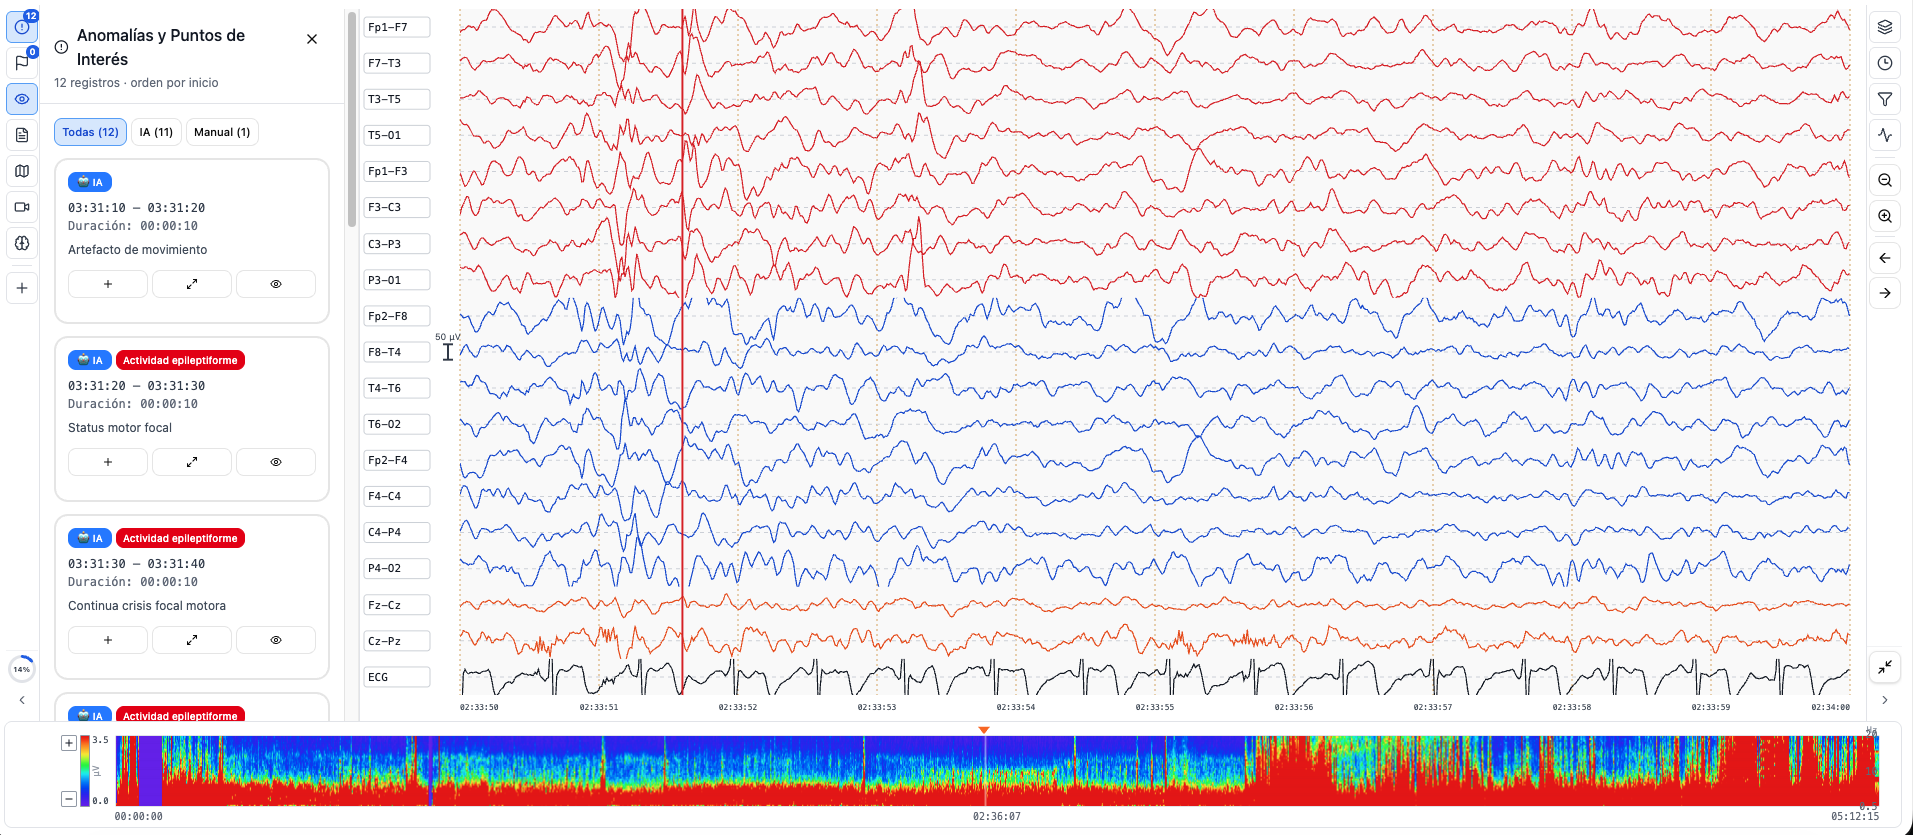
\includegraphics[width=0.95\textwidth]{Chapter6/Chapter6Figs/ia_revision_listado.png}
    \caption{Intervalos identificados por el modelo HGB~2.0 en un estudio real, clasificados y descritos por la especialista en EpilexIA.}
    \label{fig:ia-revision-listado}
\end{figure}

Por consiguiente, las pruebas realizadas permitieron verificar la integración completa entre los componentes del subsistema de IA, desde la solicitud de análisis hasta la presentación de resultados en la interfaz web.
Estas verificaciones corresponden al funcionamiento integrado del sistema sobre un conjunto reducido de estudios y no constituyen una evaluación estadística del desempeño diagnóstico del modelo.

Cabe señalar que la prueba funcional PF-10, descrita anteriormente, se realizó utilizando resultados de inteligencia artificial que ya se encontraban almacenados en la base de datos, por lo que su alcance se limita a la consulta y visualización de dichos registros. La ejecución completa del motor de IA se verificó de manera independiente mediante las pruebas descritas en esta sección.

\section{Evaluación de usabilidad}

La evaluación de usabilidad de EpilexIA incluyó sesiones de prueba con una médica especialista en epileptología del Instituto de Previsión Social (IPS), perteneciente al grupo de usuarios destinatarios de la plataforma. El propósito fue observar la interacción de la profesional con las funcionalidades relacionadas con su actividad clínica.

Durante las sesiones, la especialista realizó tareas representativas del flujo de trabajo previsto, entre ellas la carga de archivos EEG en formato EDF, la exploración de señales electroencefalográficas mediante el visualizador, el marcado manual de posibles anomalías y la elaboración del informe médico correspondiente.

Estas actividades permitieron observar la utilización directa de las herramientas disponibles y comprobar que la profesional pudo completar las tareas descritas en el escenario evaluado.

La evaluación tuvo carácter exploratorio y cualitativo. No se aplicaron cuestionarios estandarizados de usabilidad ni se realizaron mediciones sistemáticas de tiempos de ejecución, tasas de error o satisfacción de la usuaria. Por consiguiente, los resultados no permiten establecer indicadores cuantitativos de eficacia, eficiencia o satisfacción.

La realización de evaluaciones adicionales con un mayor número de profesionales y procedimientos sistemáticos de medición permitiría obtener resultados más representativos sobre la experiencia de uso de EpilexIA.

\section{Validación en el contexto del Hospital Central del IPS}

Como parte de las actividades de validación contextual de EpilexIA, se realizaron sesiones de prueba en el consultorio de una médica especialista en epileptología, ubicado en el Hospital Central del Instituto de Previsión Social (IPS).

Las sesiones se desarrollaron durante los meses de septiembre y octubre de 2026, mediante visitas semanales realizadas los días jueves, de 10:00 a 13:00, con la participación del equipo de desarrollo.
En ellas, la especialista cargó y revisó en la plataforma seis estudios EEG de pacientes del hospital, exportados en formato EDF desde el equipo de adquisición.

La profesional accedió a la plataforma, desplegada en la nube, tanto desde su propia computadora portátil, con el navegador Google Chrome, como desde los equipos del hospital, utilizando en ambos casos sus credenciales de usuario.
En el primer caso empleó su propia conexión a internet y, en el segundo, la red del hospital, lo que permitió observar el comportamiento del sistema con distintos dispositivos y condiciones de conectividad.
Los estudios cargados fueron exportados por la especialista desde el equipo de adquisición del servicio.

Durante las sesiones se desarrolló un flujo de trabajo relacionado con el análisis de estudios electroencefalográficos, cuyas actividades se describieron en la sección anterior. La experiencia proporcionó evidencia inicial de utilización de la plataforma en el contexto institucional para el cual fue concebida.

Durante las sesiones, la especialista formuló observaciones sobre el funcionamiento de la plataforma, que el equipo de desarrollo registró e incorporó de manera progresiva entre una visita y la siguiente.
El Cuadro~\ref{tab:observaciones-especialista} resume dichas observaciones, clasificadas en ajustes de experiencia de uso, corrección de errores y optimizaciones generales del sistema.
Las versiones del sistema descritas en los capítulos anteriores ya incorporan las mejoras implementadas.

\begingroup
\small
\begin{longtable}{|p{0.8cm}|p{9.6cm}|p{2.6cm}|}
\caption{Observaciones surgidas en las sesiones de validación con la especialista y estado de su incorporación.}
\label{tab:observaciones-especialista}\\
\hline
\textbf{N.º} & \textbf{Observación o mejora} & \textbf{Estado} \\
\hline
\endfirsthead

\multicolumn{3}{c}{\textit{Continuación del Cuadro~\thetable}}\\
\hline
\textbf{N.º} & \textbf{Observación o mejora} & \textbf{Estado} \\
\hline
\endhead

\multicolumn{3}{|l|}{\textbf{Ajustes de experiencia de uso}} \\
\hline
1 & Sensibilidad predeterminada de 50~$\mu$V para el canal de ECG. & Implementada \\
\hline
2 & Configuración de filtros independiente para cada canal. & Implementada \\
\hline
3 & Exclusión del canal de ECG de los filtros globales. & Implementada \\
\hline
4 & Incorporación de las derivaciones de línea media del sistema 10-20. & Implementada \\
\hline
5 & Posibilidad de desactivar un canal ante electrodos defectuosos. & Implementada \\
\hline
6 & Colores diferenciados por grupo de derivaciones y para el ECG, de forma análoga al equipo de adquisición. & Implementada \\
\hline
7 & Navegación continua del trazado mediante el teclado y el ratón. & Implementada \\
\hline
8 & Visualización del trazado completo en una única ventana, sin desplazamiento vertical. & Implementada \\
\hline
9 & Espectrograma con referencias temporales para la navegación. & Implementada \\
\hline
10 & Marcado manual de intervalos que se extienden más allá de la ventana visible. & Implementada \\
\hline
11 & Disponibilidad del video en el modo de pantalla completa. & Implementada \\
\hline
12 & Pausa y reanudación del video mediante la barra espaciadora. & Implementada \\
\hline
13 & Ventanas flotantes de tamaño ajustable para el video y el mapa de electrodos. & Implementada \\
\hline
14 & Registro automático en el informe de las anomalías incorporadas, manuales o identificadas mediante IA. & Implementada \\
\hline
15 & Consulta del informe en un panel lateral del modo de pantalla completa. & Implementada \\
\hline
16 & Ejecución del análisis de IA desde el modo de pantalla completa. & Implementada \\
\hline
17 & Avance por ventana con las flechas del teclado y avance continuo por segundo mediante el ratón. & Implementada \\
\hline
18 & Ajuste de la sensibilidad con las flechas del teclado. & Implementada \\
\hline
19 & Sincronización del video al navegar hacia un punto de interés. & Implementada \\
\hline
20 & Ampliación de las etiquetas disponibles para clasificar anomalías. & Pendiente \\
\hline
\multicolumn{3}{|l|}{\textbf{Corrección de errores}} \\
\hline
21 & Corrección de la frecuencia del filtro \textit{Notch} a 50~Hz. & Implementada \\
\hline
22 & Recorte de los trazados al área de su canal, para evitar la superposición con canales adyacentes. & Implementada \\
\hline
23 & Corrección del ordenamiento del listado de anomalías. & Implementada \\
\hline
24 & Unificación del formato de hora (HH:MM:SS). & Implementada \\
\hline
25 & Revisión de la amplitud del canal de ECG con sensibilidad de 50~$\mu$V. & Pendiente \\
\hline
\multicolumn{3}{|l|}{\textbf{Optimizaciones generales del sistema}} \\
\hline
26 & Envío de las anomalías manuales al subsistema de IA para la retroalimentación de los modelos. & Implementada \\
\hline
27 & Optimización del consumo de recursos durante la ejecución del análisis de IA. & Implementada \\
\hline
28 & Procesamiento en paralelo del análisis de IA para estudios pendientes de ejecución. & Implementada \\
\hline
29 & Inicio del análisis de IA una vez finalizadas la carga del estudio y la conversión del video, para evitar la competencia por recursos del servidor. & Implementada \\
\hline
\end{longtable}
\endgroup

No obstante, estas actividades se realizaron con una especialista y no constituyeron una validación clínica integral ni una evaluación estadística del desempeño diagnóstico. La revisión de los resultados del subsistema de inteligencia artificial se efectuó sobre un conjunto reducido de estudios.

En consecuencia, las sesiones aportaron evidencia sobre la utilización de EpilexIA en el entorno hospitalario del IPS. Para determinar su aplicabilidad clínica de manera más amplia, serían necesarias evaluaciones adicionales con otros profesionales y una mayor diversidad de estudios EEG.

Como parte de la preparación para el uso del sistema en el hospital, se elaboraron y entregaron tres documentos: un manual de usuario para los perfiles Especialista y Técnico, un manual para el equipo de TI responsable de la administración del sistema y una guía específica para la exportación y carga de estudios, que es la tarea central del personal técnico.

\section{Síntesis de la evaluación por aspectos de calidad}
\label{sec:sintesis-aspectos}

El Cuadro~\ref{tab:sintesis-aspectos} sintetiza, para cada aspecto de calidad considerado, los puntos cubiertos por las pruebas de este capítulo y por las pruebas automatizadas de los repositorios, y los que no fueron cubiertos.
La organización de la evaluación y de su reporte toma como referencia las guías GEP-HI \citep{Nykanen2011GEPHI} y STARE-HI \citep{Talmon2009STAREHI}.
Las guías y normas citadas se emplean como marco de referencia; el presente trabajo no afirma conformidad ni certificación respecto de ninguna de ellas.

\begingroup
\footnotesize
\setlength{\tabcolsep}{4pt}
\renewcommand{\arraystretch}{1.15}
\begin{longtable}{|>{\raggedright\arraybackslash}p{0.19\textwidth}|>{\raggedright\arraybackslash}p{0.46\textwidth}|>{\raggedright\arraybackslash}p{0.25\textwidth}|}
\caption{Síntesis de la evaluación de EpilexIA por aspectos de calidad.}
\label{tab:sintesis-aspectos}\\
\hline
\textbf{Aspecto y referencia} & \textbf{Puntos cubiertos y pruebas realizadas} & \textbf{Puntos no cubiertos} \\
\hline
\endfirsthead

\multicolumn{3}{c}{\textit{Continuación del Cuadro~\thetable}}\\
\hline
\textbf{Aspecto y referencia} & \textbf{Puntos cubiertos y pruebas realizadas} & \textbf{Puntos no cubiertos} \\
\hline
\endhead

\textbf{Diseño y reporte de la evaluación} \citep{Nykanen2011GEPHI,Talmon2009STAREHI} &
Definición de la estrategia y de los ámbitos de prueba; casos con procedimiento, resultado esperado y resultado obtenido; descripción del contexto, del sistema y de los participantes; declaración de limitaciones. &
Plan formal de evaluación previo a la ejecución; gestión de riesgos del estudio; reporte de la totalidad de los elementos de STARE-HI. \\
\hline

\textbf{Usabilidad} \citep{ISO9241-11:2018,Brooke1996SUS} &
Observación cualitativa, sin medición de indicadores: la especialista completó las tareas del flujo clínico en sesiones semanales durante dos meses. Contexto de uso real: equipos y red del hospital. Observaciones registradas e incorporadas (Cuadro~\ref{tab:observaciones-especialista}). Documentación entregada: manual de usuario para especialistas y técnicos, manual para el equipo de TI a cargo de la administración del sistema y guía específica de carga de estudios. &
Medición de eficacia y eficiencia (tareas completadas, tiempos y errores); satisfacción mediante el cuestionario SUS; más de un participante; perfiles Técnico y Administrador. \\
\hline

\textbf{Rendimiento} &
Sin evaluación. &
Trabajo futuro. \\
\hline

\textbf{Fiabilidad} &
Seguimiento de la actividad del motor (PI-09); comportamiento ante la indisponibilidad del servicio de IA y ante la saturación de la cola, verificado en un entorno de pruebas local (PI-15, PI-16); persistencia de la información tras cerrar y reiniciar la sesión (PF-09, PF-11, PF-13); pruebas automatizadas de los reintentos en la carga de archivos. &
Ensayos de fallos provocados durante el procesamiento. \\
\hline

\textbf{Seguridad y control de acceso} \citep{OWASP2025ASVS} &
Autenticación (PF-01, PF-02, PI-01); gestión y revocación de sesiones (PI-03); autorización por rol y por recurso, verificada también en el \textit{backend} (PF-12, PF-14, PI-02) y mediante pruebas automatizadas; registro de auditoría (PF-15, PI-14). Mecanismos de protección de datos implementados: contraseñas almacenadas mediante \textit{hash}, \textit{tokens} con vencimiento para sesiones y cuentas, enlaces para compartir estudios revocables, enmascarado de datos sensibles en los registros de ejecución, restricciones en la carga de archivos, componentes internos sin exposición a internet y comunicación mediante HTTPS. &
Verificación sistemática frente a los requisitos de la norma; pruebas de intrusión. \\
\hline

\textbf{Privacidad} &
Sin evaluación. &
Trabajo futuro. \\
\hline

\textbf{Fidelidad del visualizador} &
Sensibilidad (PF-06); montajes Doble Banana y Transversal (PF-07); filtros de corte inferior, de corte superior y \textit{Notch} (PF-08); pruebas automatizadas de filtros, unidades, escalas, eje temporal y montajes. &
Comparación cuantitativa con señales de comportamiento conocido. \\
\hline

\textbf{Interoperabilidad} \citep{Kemp1992EDF,KempOlivan2003EDFPlus} &
Lectura de registros EDF y EDF+, con pruebas automatizadas del lector; carga y procesamiento de registros exportados por el equipo de adquisición (PF-05, PI-05); seis estudios reales; conversión del video del equipo de adquisición a MP4; exportación del informe a PDF. &
Importación de las anotaciones de EDF+; comparación con un lector independiente; intercambio con otros sistemas. \\
\hline

\textbf{Accesibilidad} \citep{W3C2023WCAG22} &
Sin evaluación. &
Trabajo futuro. \\
\hline

\textbf{Trazabilidad} &
Auditoría de las acciones por usuario, con consulta y filtros (PF-15); registro de eventos del ciclo de IA (PI-14); identificador, estado y parámetros de cada ejecución (PI-06, PI-10); vínculo entre resultados, ejecución e informe (PI-11, PI-17). &
Reconstrucción documentada de una ejecución completa, del registro EEG al informe. \\
\hline

\textbf{Verificación funcional integrada} &
15 casos funcionales (PF-01 a PF-15) y 17 de integración (PI-01 a PI-17) aprobados; flujo completo sobre seis estudios reales, del registro del estudio al informe; pruebas automatizadas en los repositorios. &
Pruebas automatizadas de extremo a extremo; integración continua; otros navegadores y tamaños de pantalla. \\
\hline

\end{longtable}
\endgroup

Tres aspectos no fueron evaluados y se plantean como trabajo futuro: el rendimiento, la privacidad y la accesibilidad.
Respecto de la privacidad, el subsistema de inteligencia artificial recibe el número de documento del paciente, que se utiliza para vincular los estudios y las ejecuciones entre ambas bases de datos.
Como trabajo futuro se prevé reemplazar el documento por un identificador único sin significado.

\section[Análisis del cumplimiento de los requerimientos]{Análisis del cumplimiento de los \\requerimientos}

El análisis del cumplimiento de los requerimientos
de EpilexIA se realizó considerando las
funcionalidades implementadas y las evidencias
obtenidas durante las pruebas funcionales,
de integración y de utilización del sistema.

Las verificaciones efectuadas permitieron
comprobar el funcionamiento de los mecanismos
de autenticación y autorización, la gestión
de pacientes y estudios electroencefalográficos,
así como el almacenamiento y la visualización
de señales EEG.

Adicionalmente, durante las sesiones de prueba
realizadas con una especialista en epileptología
del IPS, se verificó la utilización de las
funcionalidades de carga de archivos EDF,
marcado manual de posibles anomalías y
elaboración de informes médicos. Esta
experiencia aportó evidencia de uso de
funciones vinculadas directamente con el
trabajo clínico de los profesionales
destinatarios del sistema.

En cuanto al subsistema de inteligencia artificial, se comprobó la disponibilidad de los servicios, la preparación de las estructuras de persistencia y la ejecución integral del procesamiento mediante IA sobre estudios reales, desde la solicitud de análisis hasta la generación, recuperación y presentación de nuevos resultados.

En términos generales, las evidencias obtenidas permiten establecer un cumplimiento verificable de los requerimientos asociados a las funcionalidades de gestión, visualización y procesamiento mediante inteligencia artificial.

Este análisis se limita a los escenarios
efectivamente evaluados y no implica que
todos los requerimientos del sistema hayan
sido comprobados exhaustivamente.

\begin{nuevotexto}
El análisis de estos resultados respecto de los objetivos del trabajo y de la hipótesis planteada se desarrolla en el Capítulo~\ref{chap:conclusiones}.
\end{nuevotexto}


\clearpage
\lhead{\emph{Conclusiones y trabajos futuros}}
\chapter{Conclusiones y trabajos futuros}
\label{chap:conclusiones}

\markboth{\hfill \thechapter. Conclusiones y trabajos futuros}{\hfill \thechapter. Conclusiones y trabajos futuros}

Este capítulo presenta las conclusiones derivadas del desarrollo y la evaluación de EpilexIA.
En primer lugar se exponen las conclusiones generales del trabajo.
Luego se analiza el cumplimiento de los objetivos definidos en la Sección~\ref{sec:objetivos} y se contrasta la hipótesis formulada en la Sección~\ref{sec:hipotesis} con las evidencias reunidas en el Capítulo~\ref{pruebas_evaluacion}.
Posteriormente se identifican los principales aportes y las limitaciones del proyecto y, a partir de estas últimas, se proponen las líneas de trabajo futuro.

Las afirmaciones de este capítulo se restringen a lo que las evidencias documentadas permiten sostener.
En consecuencia, se distingue entre la verificación del funcionamiento del sistema, realizada sobre un conjunto reducido de estudios en condiciones controladas, y una validación clínica de alcance general, que excede el presente trabajo.


\section{Conclusiones generales}
\label{sec:conclusiones-generales}

El presente trabajo se propuso desarrollar un sistema web de apoyo a la detección de crisis epilépticas mediante el análisis de señales EEG asistido por inteligencia artificial, que complementara el flujo de trabajo posterior a la adquisición de los estudios en el área de Neurología del Hospital Central del Instituto de Previsión Social (IPS).
Como resultado se obtuvo EpilexIA, una plataforma que reúne en un mismo entorno la gestión de pacientes y estudios EEG, la visualización interactiva de las señales, el registro de anomalías, la presentación de las anomalías identificadas por el componente de inteligencia artificial, la elaboración de informes médicos, el control de acceso basado en roles y la auditoría de las operaciones realizadas.

El desarrollo se condujo mediante una adaptación del Modelo V \citep{ForsbergMooz1991}, que permitió mantener la correspondencia entre las necesidades relevadas, las decisiones de diseño, las funcionalidades implementadas y las pruebas destinadas a comprobarlas.
El relevamiento realizado con profesionales del área dio lugar a 64 requerimientos funcionales, organizados en siete áreas, y a 16 requerimientos no funcionales, que sirvieron de referencia para el diseño presentado en el Capítulo~4 y para la definición de los casos de prueba del Capítulo~\ref{pruebas_evaluacion}.
La incorporación de ciclos de retroalimentación resultó adecuada para un contexto en el que la disponibilidad de los profesionales condicionaba las instancias de relevamiento y revisión.
Esto se observó particularmente en el visualizador EEG, cuya definición evolucionó a partir de las observaciones realizadas por la médica especialista durante las sesiones de trabajo semanales (Cuadro~\ref{tab:observaciones-especialista}).

Desde el punto de vista arquitectónico, la decisión de separar la gestión de la información clínica del subsistema de inteligencia artificial, coordinando este último mediante una API específica y una cola persistente de ejecuciones, demostró ser pertinente.
Esta separación permitió desarrollar y verificar las funcionalidades de gestión y visualización con independencia de la evolución del procesamiento automatizado, e incorporar posteriormente el modelo HGB~2.0 en reemplazo del anterior sin modificar la gestión clínica.
Asimismo, mantiene diferenciados los resultados producidos por el modelo de las decisiones registradas por el especialista.

Las evidencias obtenidas respaldan el funcionamiento de la plataforma.
Los quince casos de prueba funcional definidos resultaron aprobados (Cuadro~\ref{tab:sintesis_pruebas_funcionales}).
Los diecisiete casos de prueba de integración resultaron igualmente aprobados: verificaron la autenticación, la protección de los servicios, la revocación de sesiones, la persistencia de pacientes, estudios y archivos EEG, y el ciclo completo de procesamiento mediante inteligencia artificial (Cuadro~\ref{tab:resumen_pruebas_integracion}).
La suite automatizada del \textit{frontend}, compuesta por 216 casos, se ejecutó sin fallos (Cuadro~\ref{tab:pruebas-frontend}).

A ello se suma la verificación integral realizada con registros clínicos reales.
En condiciones controladas, se procesaron en la plataforma seis estudios EEG correspondientes a pacientes del Hospital Central del IPS, cargados en formato EDF tal como los exporta el equipo de adquisición, ejecutando el ciclo completo de análisis: carga del registro, solicitud de procesamiento, ejecución del modelo, persistencia de los resultados y presentación de las anomalías en el visualizador.
En todos los casos el ciclo se completó y los intervalos identificados por el modelo se presentaron correctamente sobre el registro EEG.

Los resultados del análisis automatizado fueron revisados por la médica especialista en epileptología durante las sesiones de validación realizadas en el hospital.
La especialista clasificó los intervalos señalados por el modelo y confirmó la mayor parte de ellos como anomalías.
En uno de los estudios, por ejemplo, de once intervalos señalados la especialista confirmó diez, identificó el restante como un artefacto de movimiento y agregó manualmente una anomalía (Figuras~\ref{fig:ia-revision-listado} y~\ref{fig:ia-revision-manual}).
Todas las ejecuciones se realizaron con el modelo de detección vigente, denominado HGB~2.0 y basado en \textit{Gradient Boosting} (Sección~\ref{subsec:modelo-vigente-hgb}), que reemplazó al modelo utilizado en las etapas iniciales del proyecto.
Este modelo opera con un umbral de probabilidad de 0,95 y requiere dos ventanas consecutivas por encima de dicho umbral para señalar un intervalo.

En síntesis, EpilexIA constituye una plataforma funcional en todos sus componentes, incluida la detección de anomalías asistida por inteligencia artificial, cuyo funcionamiento fue verificado de extremo a extremo con estudios reales y revisado por una especialista del área.
A la fecha de redacción de este documento, el sistema opera en la infraestructura en la nube provista por BigQ (Sección~\ref{subsec:despliegue-nube}), donde se realizaron las validaciones con la especialista, y se encuentra en proceso de transferencia al IPS para su utilización por los profesionales responsables de la revisión de estudios EEG.


\section{Cumplimiento de los objetivos}
\label{sec:cumplimiento-objetivos}

El Cuadro~\ref{tab:cumplimiento-objetivos} resume el grado de cumplimiento de los objetivos específicos planteados en la Sección~\ref{subsec:objetivos-especificos}, junto con las evidencias que lo sustentan.

\begingroup
\small
\setlength{\tabcolsep}{4pt}
\renewcommand{\arraystretch}{1.2}

\begin{longtable}{|
>{\raggedright\arraybackslash}p{0.27\textwidth}|
>{\raggedright\arraybackslash}p{0.43\textwidth}|
>{\raggedright\arraybackslash}p{0.20\textwidth}|}
\caption{Cumplimiento de los objetivos específicos de EpilexIA.}
\label{tab:cumplimiento-objetivos}\\
\hline
\textbf{Objetivo específico} &
\textbf{Evidencia} &
\textbf{Cumplimiento} \\
\hline
\endfirsthead

\multicolumn{3}{c}{\textit{Continuación del Cuadro~\thetable}}\\
\hline
\textbf{Objetivo específico} &
\textbf{Evidencia} &
\textbf{Cumplimiento} \\
\hline
\endhead

1. Relevar el estado del arte. &
Capítulo~2: revisión de SaMD, electroencefalografía, procesamiento de señales, inteligencia artificial aplicada al EEG y herramientas existentes, con una comparación respecto de EpilexIA (Cuadro~\ref{tab:comparacion-herramientas-eeg}). &
Cumplido. \\
\hline

2. Analizar los requerimientos funcionales y no funcionales. &
Capítulo~4: contexto operativo, actores, 64 requerimientos funcionales y 16 no funcionales derivados del relevamiento en el Hospital Central del IPS. &
Cumplido. \\
\hline

3. Diseñar e implementar la base de datos relacional. &
Capítulos~4 y~5: modelo de datos clínicos y del procesamiento de IA implementado en PostgreSQL.
Persistencia verificada en las pruebas PI-04 y PI-05. &
Cumplido. \\
\hline

4. Desarrollar el \textit{backend} REST con control de acceso e integración con el servicio de IA. &
Capítulo~5: servicios implementados con Spring Boot.
Autenticación, autorización y roles verificados en PF-01, PF-02, PF-12 a PF-14 y PI-01 a PI-03.
Integración con la API de IA verificada en PI-06 a PI-17 y mediante la ejecución del ciclo completo de análisis sobre estudios reales. &
Cumplido. \\
\hline

5. Construir el \textit{frontend} web con visualizador EEG, gestión de anomalías, informes y auditoría. &
Capítulo~5: interfaz implementada con React y TypeScript; 216 pruebas automatizadas aprobadas.
Funcionalidades verificadas en PF-03 a PF-11 y PF-15.
La utilización desde \textit{tablets} no fue evaluada de manera sistemática. &
Cumplido; uso en \textit{tablets} sin evaluación formal. \\
\hline

6. Evaluar el sistema mediante pruebas funcionales, de usabilidad e integración con registros EEG reales. &
Capítulo~\ref{pruebas_evaluacion}: pruebas funcionales y de integración; verificación integral con estudios EEG reales del Hospital Central del IPS; sesiones de uso con una médica especialista.
La usabilidad se evaluó de forma cualitativa y no se realizaron mediciones sistemáticas de rendimiento. &
Cumplido; usabilidad evaluada cualitativamente. \\
\hline

\end{longtable}
\endgroup

Los objetivos específicos 1 y 2 se cumplieron mediante la revisión presentada en el Capítulo~2 y el análisis desarrollado en el Capítulo~4.
La revisión permitió ubicar a EpilexIA respecto de las herramientas utilizadas en el ámbito clínico y de los antecedentes de detección automatizada de crisis, mientras que el relevamiento identificó las necesidades de acceso, integración de la información y trazabilidad que orientaron el diseño.

Los objetivos 3, 4 y 5, relativos a la construcción de la plataforma, se consideran cumplidos.
La base de datos, el \textit{backend} y el \textit{frontend} fueron implementados e integrados, y su funcionamiento fue verificado mediante las pruebas funcionales y de integración ejecutadas.
La integración con el servicio de inteligencia artificial quedó comprobada al completarse el ciclo de análisis sobre estudios reales.
La única salvedad corresponde a la utilización de la interfaz desde \textit{tablets}, que fue contemplada en el diseño pero no evaluada de forma sistemática.

El objetivo 6 se considera cumplido en cuanto a las pruebas funcionales, las pruebas de integración y la utilización de registros EEG reales del hospital.
La evaluación de usabilidad se apoyó en las sesiones realizadas con la médica especialista y tuvo carácter cualitativo, sin aplicación de instrumentos estandarizados.

En relación con el objetivo general, se desarrolló un sistema web que permite gestionar pacientes, estudios EEG e informes clínicos, y visualizar las anomalías identificadas por el componente de inteligencia artificial integrado.
El sistema complementa el flujo de trabajo existente con Easy Cadwell III, cuyos registros exportados en formato EDF constituyen su información de entrada.
Por tanto, el objetivo general se considera alcanzado.


\section{Contrastación de la hipótesis}
\label{sec:contrastacion-hipotesis}

La hipótesis del proyecto sostiene que un sistema web integrado, que centralice la gestión de pacientes, estudios EEG e informes clínicos e incorpore la visualización de resultados del procesamiento mediante inteligencia artificial, puede contribuir a mejorar el flujo de trabajo relacionado con el análisis de estudios electroencefalográficos.
Para contrastarla, resulta conveniente considerar por separado los beneficios que la hipótesis anticipa.

\begin{itemize}
    \item \textbf{Acceso a los estudios desde diferentes dispositivos.}
    Durante las sesiones realizadas en el Hospital Central del IPS, la especialista accedió a la plataforma tanto desde su propio equipo portátil como desde los equipos del hospital, mediante un navegador web, sin instalar software adicional y con distintas conexiones de red.
    Esta evidencia respalda el beneficio previsto para computadoras y \textit{notebooks}.
    La utilización desde \textit{tablets} no fue evaluada.

    \item \textbf{Trazabilidad de las actividades.}
    Las pruebas funcionales y de integración verificaron el control de acceso según roles, la restricción de edición y el cierre de los informes, la revocación de sesiones y la consulta del historial de auditoría.
    Estos resultados respaldan la capacidad del sistema para registrar y delimitar las acciones de los usuarios.

    \item \textbf{Apoyo para la localización y evaluación de segmentos de interés.}
    En los estudios reales procesados, la plataforma presentó los intervalos identificados por el modelo y permitió navegar directamente hacia ellos.
    La especialista confirmó como anomalías la mayor parte de los intervalos señalados y complementó los resultados con registros manuales cuando lo consideró necesario.
    Esta evidencia respalda el beneficio previsto dentro del conjunto de estudios evaluado.

    \item \textbf{Facilitación de la revisión y la elaboración de informes.}
    La especialista completó en un mismo entorno la carga del estudio, la revisión de las señales, el registro de anomalías y la elaboración del informe.
    El trabajo no incluyó mediciones de tiempos que permitan cuantificar este beneficio.
\end{itemize}

A partir de este análisis, la hipótesis se considera \textbf{corroborada dentro del alcance de la evaluación realizada}.
Las evidencias respaldan que el sistema proporciona acceso, organización y trazabilidad sobre las actividades posteriores a la adquisición del EEG, y que los resultados del procesamiento mediante inteligencia artificial orientaron la revisión de los registros evaluados.
La magnitud de la mejora sobre el flujo de trabajo y su generalización a un volumen mayor de estudios y de profesionales deberán establecerse durante la etapa de uso productivo.
En todos los casos, la interpretación de los registros y las decisiones clínicas permanecieron bajo la responsabilidad de la especialista, conforme a lo previsto en la hipótesis.


\section{Aportes del trabajo}
\label{sec:aportes}

Los principales aportes del presente trabajo son los siguientes:

\begin{itemize}
    \item \textbf{Una plataforma web integrada para el flujo posterior a la adquisición del EEG.}
    EpilexIA reúne en un único entorno, accesible mediante navegador, funciones que en el flujo relevado se encontraban distribuidas entre distintas herramientas: gestión de pacientes y estudios, revisión de señales, registro de anomalías y elaboración de informes por especialista.
    La plataforma complementa al sistema de adquisición existente, sin sustituirlo.

    \item \textbf{Un visualizador EEG para entornos web.}
    El visualizador implementa en el navegador operaciones propias de la revisión electroencefalográfica, como la selección de montajes, la aplicación de filtros, el ajuste de sensibilidad, la navegación temporal y la reproducción sincronizada de video, e incorpora mecanismos de carga segmentada para el tratamiento de registros extensos.

    \item \textbf{La integración operativa de un modelo de detección en el flujo clínico.}
    El trabajo lleva un modelo de aprendizaje automático desde su artefacto entrenado hasta su utilización por una especialista sobre estudios reales, y da continuidad a los antecedentes desarrollados en la FP-UNA sobre detección automática de crisis \citep{AyalaBritez2026SeizureDetection,Lezcano2026GradientBoosting}.

    \item \textbf{Una arquitectura desacoplada para el procesamiento mediante inteligencia artificial.}
    La separación entre el \textit{backend} clínico, la API de IA y el motor de procesamiento, coordinados mediante una cola persistente, permite incorporar o reemplazar modelos sin modificar la gestión clínica.

    \item \textbf{Un diseño que preserva la supervisión profesional.}
    El sistema mantiene diferenciados los intervalos identificados automáticamente de los hallazgos confirmados por el especialista, asigna la responsabilidad de cada informe a su autor y conserva las anotaciones manuales y las ventanas incorporadas a los informes.
    Este criterio es consistente con las consideraciones sobre software de apoyo a la decisión clínica revisadas en el Capítulo~2 \citep{IMDRF2013SaMD,FDA2026CDS}, y deja disponibles datos de retroalimentación clínica que pueden emplearse en la mejora posterior de los modelos.

    \item \textbf{Un sistema en condiciones de ser transferido a la institución destinataria.}
    El resultado del trabajo no se limita a un prototipo: la plataforma fue utilizada con estudios reales en el entorno hospitalario y se encuentra en proceso de transferencia al IPS.
\end{itemize}


\section{Limitaciones}
\label{sec:limitaciones}

Las conclusiones de este trabajo deben interpretarse considerando las siguientes limitaciones:

\begin{itemize}
    \item \textbf{Tamaño y condiciones de la verificación con estudios reales.}
    La verificación del análisis automatizado se realizó sobre un conjunto reducido de estudios, en condiciones controladas y con la revisión de una única especialista.
    Sus resultados muestran que el sistema funciona de extremo a extremo y que las detecciones resultaron clínicamente pertinentes en esos estudios, pero no constituyen una validación clínica ni permiten estimar con significación estadística la sensibilidad o la especificidad del modelo.

    \item \textbf{Alcance respecto del modelo de inteligencia artificial.}
    El desarrollo y el entrenamiento del modelo no forman parte del alcance del trabajo.
    Su comportamiento ante otros equipos de adquisición, configuraciones de registro o poblaciones de pacientes no fue evaluado.

    \item \textbf{Evaluación de usabilidad.}
    La evaluación con usuarios tuvo carácter cualitativo, sin cuestionarios estandarizados ni medición de indicadores de eficacia, eficiencia o satisfacción.
    Los perfiles Técnico y Administrador no fueron evaluados con usuarios del hospital; su primera utilización por personal del IPS tendrá lugar en las capacitaciones programadas para fines de noviembre de 2026 (Sección~\ref{subsec:actividades-en-curso}).

    \item \textbf{Ausencia de mediciones sistemáticas de rendimiento.}
    No se documentaron tiempos de respuesta, consumo de recursos ni comportamiento bajo carga concurrente.

    \item \textbf{Privacidad y accesibilidad sin evaluar.}
    Estos aspectos no fueron evaluados (Cuadro~\ref{tab:sintesis-aspectos}).
    En particular, el subsistema de inteligencia artificial recibe el número de documento del paciente, que se utiliza para vincular los estudios entre ambas bases de datos.

    \item \textbf{Cobertura de las pruebas.}
    Las pruebas automatizadas utilizan dependencias simuladas y no existen pruebas automatizadas de extremo a extremo ni medición formal de cobertura.
    Las pruebas funcionales verificaron el control de acceso, pero no constituyen una evaluación integral de la seguridad del sistema.

    \item \textbf{Compatibilidad con dispositivos.}
    La utilización desde \textit{tablets}, prevista en los objetivos, no fue evaluada de manera sistemática.

    \item \textbf{Situación respecto del marco de dispositivos médicos.}
    EpilexIA fue concebido considerando los conceptos de software como dispositivo médico, pero el trabajo no comprendió una categorización formal de riesgo ni un proceso de evaluación de conformidad regulatoria.

    \item \textbf{Contexto de validación.}
    Los requerimientos y la validación se circunscriben al área de Neurología del Hospital Central del IPS.
    Su utilización en otros entornos clínicos requeriría nuevos relevamientos y procesos de validación.
\end{itemize}


\section{Trabajos futuros}
\label{sec:trabajos-futuros}

Concluidas la implementación y la verificación del sistema, la etapa siguiente corresponde a su uso productivo en la institución destinataria.
Se distinguen las actividades de transferencia que ya se encuentran en curso de las líneas de trabajo que quedan abiertas.

\subsection{Actividades de transferencia en curso}
\label{subsec:actividades-en-curso}

\begin{itemize}
    \item \textbf{Transferencia al IPS y uso productivo.}
    Completar el proceso de transferencia del sistema, actualmente en curso.
    El IPS dispondrá servidores propios y el equipo de desarrollo, junto con BigQ, realizará el respaldo de la información y el despliegue, en la infraestructura institucional, de la versión validada con la especialista, de modo que pueda ser utilizada por todos los profesionales responsables de la revisión de estudios EEG.
    En esta etapa se prevé que la especialista utilice la plataforma de manera habitual sobre un volumen creciente de estudios, con una asistencia técnica progresivamente menor por parte del equipo de desarrollo.

    \item \textbf{Capacitación de los usuarios del IPS.}
    Como parte de la transferencia, las jornadas de capacitación para los dos perfiles que aún no utilizaron el sistema en el hospital están programadas para fines de noviembre de 2026.
    El equipo de TI del IPS será capacitado en el perfil Administrador: ingreso al sistema, creación de usuarios y restablecimiento de contraseñas de técnicos y especialistas.
    El personal de enfermería del área de Neurología será capacitado en el perfil Técnico: registro de pacientes y carga de nuevos estudios, de modo que estos queden disponibles para su análisis por los especialistas, conforme al flujo de trabajo para el cual fue diseñado el sistema.
    Las capacitaciones se apoyan en los manuales entregados para cada perfil.

    \item \textbf{Plan de mantenimiento y soporte.}
    Establecer un plan de mantenimiento que contemple la atención de incidencias, las correcciones y los ajustes menores que surjan del uso cotidiano, incluidas las observaciones de la especialista aún pendientes (Cuadro~\ref{tab:observaciones-especialista}).

\end{itemize}

\subsection{Líneas de trabajo futuro}
\label{subsec:lineas-futuras}

Las siguientes líneas atienden las limitaciones identificadas en la Sección~\ref{sec:limitaciones} y los puntos no cubiertos que se detallan en el Cuadro~\ref{tab:sintesis-aspectos}:

\begin{itemize}
    \item \textbf{Seguimiento del desempeño del modelo en condiciones de uso real.}
    Aprovechar el uso productivo para ampliar la evaluación del análisis automatizado a un mayor número de estudios y de especialistas, registrando de manera sistemática las detecciones confirmadas, las descartadas y los hallazgos no señalados por el modelo, de modo que puedan estimarse métricas como la sensibilidad, la especificidad y la tasa de falsas detecciones.

    \item \textbf{Mejora continua de los modelos.}
    Utilizar las anotaciones manuales y las ventanas confirmadas en los informes como datos para el reentrenamiento y la evaluación de nuevas versiones del modelo.

    \item \textbf{Evaluación formal de usabilidad.}
    Aplicar, durante la adopción del sistema, un protocolo de tareas representativas con los tres perfiles de usuario, midiendo la eficacia, la eficiencia y la satisfacción conforme a la norma ISO~9241-11 \citep{ISO9241-11:2018} e incorporando un instrumento estandarizado como el cuestionario \textit{System Usability Scale} \citep{Brooke1996SUS}.

    \item \textbf{Pruebas de rendimiento y compatibilidad.}
    Medir tiempos de respuesta y consumo de recursos con registros de larga duración y bajo carga concurrente, y evaluar el comportamiento de la interfaz en \textit{tablets} y en distintos navegadores.

    \item \textbf{Fortalecimiento de la verificación.}
    Incorporar pruebas automatizadas de extremo a extremo y medición de cobertura, y realizar una evaluación específica de seguridad.

    \item \textbf{Privacidad.}
    Reemplazar el número de documento del paciente que se transmite al subsistema de inteligencia artificial por un identificador único sin significado.

    \item \textbf{Accesibilidad.}
    Definir los criterios de accesibilidad aplicables a la interfaz y revisarlos tomando como referencia las pautas WCAG~2.2 \citep{W3C2023WCAG22}.

    \item \textbf{Herramientas de apoyo al desarrollo.}
    Incorporar, para el desarrollo de funcionalidades futuras, herramientas actuales de desarrollo guiado por pruebas o por especificaciones, que complementen las prácticas de desarrollo asistido por inteligencia artificial descritas en la Sección~\ref{sec:desarrollo-asistido-ia}.

    \item \textbf{Adecuación al marco de dispositivos médicos.}
    Determinar la categoría de riesgo del sistema según el marco propuesto por el IMDRF \citep{IMDRF2014SaMDRisk}, adoptar un proceso de ciclo de vida del software conforme a la norma IEC~62304 \citep{IEC62304:2006} y analizar los requisitos de la autoridad sanitaria nacional aplicables a este tipo de software.

    \item \textbf{Ampliación del alcance.}
    Analizar la interoperabilidad con los sistemas de información institucionales y la adaptación del sistema a otros servicios o centros asistenciales, con los relevamientos y validaciones que cada contexto requiera.
\end{itemize}


\section{Consideraciones finales}
\label{sec:consideraciones-finales}

El desarrollo de EpilexIA muestra que es posible construir, con tecnologías de código abierto y en estrecha relación con los profesionales destinatarios, una plataforma web que integra las actividades posteriores a la adquisición del EEG e incorpora la detección de anomalías asistida por inteligencia artificial como apoyo a la revisión del especialista.
El sistema fue verificado de extremo a extremo con estudios reales, sus resultados fueron revisados por una médica especialista en su entorno habitual de trabajo y se encuentra en proceso de transferencia a la institución para la cual fue concebido.

El proyecto muestra además el valor de la articulación entre la cooperación internacional, la academia y el sector privado para atender una necesidad de una institución pública de salud.

El trabajo deja, en consecuencia, un sistema funcional y en vías de adopción, junto con un conjunto delimitado de actividades de seguimiento, mantenimiento y evaluación que orientan su continuidad durante la etapa de uso productivo.


\clearpage
\lhead{\emph{Referencias}}
\bibliographystyle{apacite}
\bibliography{References/references}
\end{document}



\textbf{
    {\huge
        \begin{center}
        \part[Marco Teórico]{
            Marco Teórico \\ 
            \huge{}}
        \end{center}
    }
}




\clearpage
\lhead{\emph{Conclusiones y Trabajos Futuros}} 
\renewcommand\chaptername{Capítulo}%título "Capítulo"
\input{Conclusion/conclusion} % Conclusión


%% --------------- Anexo --------------------------------------
\lhead{\emph{Anexo}}
\addtotoc{Anexo}

% ============================================================
% ANEXOS - EPILEXIA
% ============================================================

\chapter*{Anexos}
\addcontentsline{toc}{chapter}{Anexos}

% En esta sección se incorporará documentación
% complementaria del sistema EpilexIA, cuando
% corresponda.


\backmatter
%% --------------- Referencias ------------------------------------

\lhead{\emph{Referencias}}
\renewcommand{\bibname}{Referencias}
\bibliography{References/references}
\bibliographystyle{alpha}

\end{document}  % The End
%% ----------------------------------------------------------------
